\documentclass[EJP,preprint]{ejpecp}
% Occupation law of a lattice Levy walk at every point.
% The class ejpecp is in TeX Live.
% This file is the arXiv version. Build: pdflatex problem131_levy_arxiv.tex, three times.
% The journal version is problem131_levy.tex, a driver that sets \arxivbuildfalse and inputs
% this file. The switch \ifarxivbuild marks the material that only the arXiv version carries.
\expandafter\ifx\csname ifarxivbuild\endcsname\relax
  \expandafter\newif\csname ifarxivbuild\endcsname
  \csname arxivbuildtrue\endcsname
\fi

\usepackage{booktabs}
\usepackage[shortlabels]{enumitem}

% ---------- theorem environments (the class provides theorem, lemma,
% proposition, corollary, definition, example, remark, hypothesis and its other
% theorem-like environments, numbered within sections; the lettered main
% theorems are added here) ----------
\theoremstyle{ejpecpbodyit}
\newtheorem{introtheorem}{Theorem}
\renewcommand{\theintrotheorem}{\Alph{introtheorem}}

% ---------- notation macros ----------
\newcommand{\Z}{\mathbb{Z}}
\newcommand{\N}{\mathbb{N}}
\newcommand{\R}{\mathbb{R}}
\newcommand{\E}{\mathbb{E}}
\newcommand{\Prob}{\mathbb{P}}
\newcommand{\Var}{\operatorname{Var}}
\newcommand{\RV}{\mathrm{RV}}
\newcommand{\ones}{\mathbf{1}}
\newcommand{\plus}{{+}}
\newcommand{\minus}{{-}}
\newcommand{\sgn}{\sigma}
\newcommand{\osgn}{\bar\sigma}

\graphicspath{{figures/}}
\emergencystretch=1em

\TITLE{Local laws for the occupation time of on/off processes with heavy-tailed, finite-mean periods: bulk, big jumps, boundary layers and aging}
\SHORTTITLE{Local laws for the occupation time of an on/off process}
\AUTHORS{Arjun Pemmasani\footnote{Department of Mathematics, Harvey Mudd College,
Claremont, CA 91711, USA. \BEMAIL{apemmasani@hmc.edu}}}
\KEYWORDS{on/off process; alternating renewal process; occupation time; L\'evy walk; local
limit theorem; stable law; big-jump principle; infinite density; aging; renewal theorem;
number of modes; switchback experiment; busy period}
\AMSSUBJ{60K05; 60G50; 60F05}
\AMSSUBJSECONDARY{60G52; 60K15; 60K25; 60F10; 82C41}
\SUBMITTED{}
\ACCEPTED{}
\ABSTRACT{Let $A_N$ be the number of time slots spent in the on state during the first $N$
slots of a discrete-time on/off process whose on and off periods are independent and have
regularly varying tails with indices in $(1,2)$. Equivalently, $A_N$ counts the right steps
of a lattice L\'evy walk. The limit law of $A_N$ at the scale $N^{1/\alpha}$ is stable and
classical. We describe $\Prob(A_N=k)$ at every point. In the bulk it is a stable density,
uniformly over the whole range, under regular variation and aperiodicity alone. On each side
of the bulk and up to the endpoint one kernel gives the law under local regular variation. It
adds a complete giant period and the period in progress at time $N$, and it contains a
renewal boundary layer at each end and an atom at each endpoint. This is a lattice form of
the infinite density of the L\'evy walk. We find the exact effect of an arbitrary initial
period on each piece, and the effect of aging, when the process is observed from time
$\theta N$ on. The bulk does not age. The atom, the layer and the big-jump zone do, and we
give their aged forms in closed form. For the stationary start and for every aged start, the
most likely value of $A_N$ is an endpoint for all large $N$ when the index is below the
golden ratio and is interior when it is above. For fresh and fair starts, aperiodic periods,
comparable scales, a second-order smoothness condition and no ties in the boundary profiles,
the law has, for all large $N$, one more mode than the two boundary profiles have local
maxima. Hence it has 3 modes for strictly log-convex period laws. The results give the
exposure law of an experiment that switches arm at the regenerations of a slotted queue with
heavy-tailed service. We prove that the cycle law of the queue satisfies the smoothness
conditions, so the mode count applies to it.}

\begin{document}

\section{Introduction}\label{sec:intro}

A lattice L\'evy walk moves on $\Z$ in runs of alternating direction. The
run lengths are independent, and their tails are regularly varying with an
index $\alpha$ between $1$ and $2$, so a run has a finite mean and an
infinite variance. Let $A_N$ be the number of right steps among the first
$N$. The position of the walk after $N$ steps is $2A_N-N$, so the law
$P_N(k)=\Prob(A_N=k)$ on $\{0,\dots,N\}$ is the law of the walk read on its
natural lattice. L\'evy walks are a standard model of
superdiffusion~\cite{zdk2015}, and the same walk describes heat transport in
one-dimensional lattices~\cite{dsd2013,wlh2016} and the occupation time of an
alternating renewal process~\cite{godrecheluck2001,lamperti1958}. Its
profile has a central peak and two ballistic side
peaks~\cite{zdh2011,dzh2012}, and the physics literature describes the part
between them by an infinite density~\cite{rdhb2014,rdhb2014b}. We describe
$P_N(k)$ for every $k$, with proofs, with one exception that we state below.

\subsection{The picture}\label{sec:intro-picture}

Figure~\ref{fig:atlas} shows $P_N$ for $N=5000$ on a logarithmic scale.
Four pieces make up the row. We call the right steps plus slots.
\begin{itemize}[nosep]
\item The bulk. Near $pN$, where $p$ is the long-run fraction of plus
slots, the law is a stable density at the scale $B_N$ of the larger of the
two run-length fluctuations. Here $B_N$ grows like $N^{1/\alpha_*}$ up to a
slowly varying factor, with $\alpha_*$ the smaller index.
\item The big-jump zones. A count $k$ with $k-pN$ much larger than $B_N$
needs one plus run of macroscopic length, a giant run, and the law of that run
gives the bin its size, which is of order $T_\plus(N)$ on the ballistic range,
with $T_\plus$ the tail of a plus run. The giant run is either complete and lies
in the interior or the final run, censored at slot $N$, and the bin is the sum
of the two contributions.
\item The boundary layers. At $k=N-j$ with $j$ fixed, the giant run is the
final one, and the only question is where it started. It starts right after the $j$-th minus slot exactly when a
minus run ends there, so the layer is $T_\plus(N)$ times the renewal mass
function $u_\minus(j)$ of the minus runs.
\item The atoms. The bin $k=N$ is the event that the first run covers the
row, and its mass is the tail of the first run.
\end{itemize}
The first run is the preparation of the walk. It may be a fresh run, a run
seen from a typical time, or anything else, and it enters each of the four
pieces through its own criterion.

\begin{figure}[t]
\centering
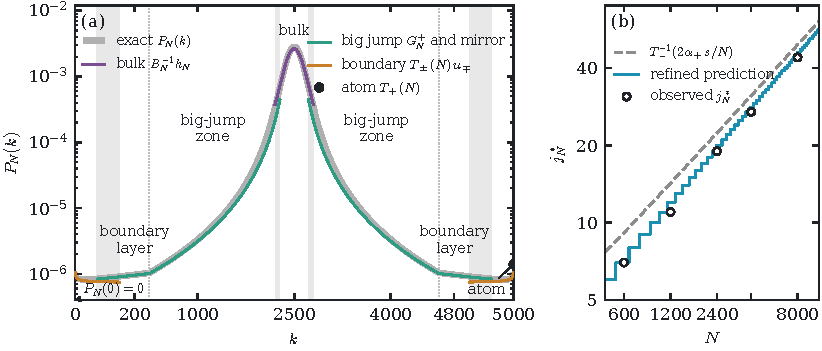
\includegraphics[width=\textwidth]{atlas}
\caption{(a) The law $P_N(k)$ for $N=5000$, run lengths with
$f(n)\propto n^{-5/2}$ for both signs and a fresh plus start, on a
logarithmic scale, with the four pieces of Theorems~\ref{thm:bulk}
and~\ref{thm:bigjump}. The two ends of the horizontal axis are stretched.
(b) The position $j^*_N$ of the interior minimum near the plus end against
$N$, on logarithmic axes, with the law of Theorem~\ref{thm:antimode} and the
refined prediction with $C(j)$ from Theorem~\ref{thm:second-order}.
Section~\ref{sec:verify} describes the computations.}
\label{fig:atlas}
\end{figure}

\subsection{Results}\label{sec:intro-results}

We state the hypotheses in Section~\ref{sec:hypotheses}. They are regular
variation of the two tails with indices in $(1,2)$, written (RV), the local
form $f_\sgn(n)\sim\alpha_\sgn T_\sgn(n)/n$ of the mass functions, written
(LR), and aperiodicity, written (SPAN). The run laws may differ between the
two signs, so the two stable scales $b_{\plus,N}$ and $b_{\minus,N}$ may
differ, and their ratio may oscillate. Every theorem below holds for every
relation between the two scales. When the smaller scale is smaller than the
other by an unbounded factor, one window on the side of the sign with the
smaller scale is described only in part, as we say below. When the ratio of
the scales stays bounded, Theorem A covers that window. The model is
symmetric, so the side in question is the plus side when the plus scale is the
smaller one and the minus side otherwise. We write $s$ for the sum of the two mean run lengths and $p$
for the fraction of the plus mean.

\emph{The bulk.} Theorem~\ref{thm:bulk} says that for a fresh start, under
(RV) and (SPAN),
\[
 \sup_{k\in\Z}\bigl|B_NP_N(k)-h_N\bigl((k-pN)/B_N\bigr)\bigr|\to0,
 \qquad \sup_kP_N(k)\le\frac C{B_N},
\]
where $h_N$ is the density of $(1-p)\theta_{\plus,N}Z_\plus-p\,\theta_{\minus,N}Z_\minus$,
with $Z_\pm$ independent totally skewed stable variables. The supremum runs
over the whole row. On a window $|k-pN|\le KB_N$ the local limit also follows
from a strong renewal theorem of Berger, and what is new is the uniformity over
every bin under (RV) and (SPAN) alone. Outside the bulk the theorem says only that
every bin is
$o(1/B_N)$, and the next theorem says what the bins are.

\emph{Big jumps and the boundary layer.} Put $L_k=(k-pN)/(1-p)$, the length
of the plus run that carries a typical configuration to the count $k$.
Theorem~\ref{thm:bigjump} says that for a fresh plus start, under (RV) and
(SPAN) for both signs and (LR) for the plus sign,
\[
 P_N(k)=\Bigl[\gamma(N-k)\,f_\plus(\lfloor L_k\rfloor)+T_\plus(\lfloor L_k\rfloor)\,u_\minus(N-k)\Bigr](1+o(1))
\]
uniformly on $pN+K\lambda_NB_N\le k\le N$, in the sense that the error
tends to zero as $N\to\infty$ and then $K\to\infty$. Here $\gamma(j)$ is an
explicit finite sum with $\gamma(j)\sim js/\mu_\minus^2$, and
$\lambda_N=1+\log(B_N/b_{\plus,N})$, which equals $1$ when the plus scale is the
larger one. The first term is a complete giant
run and the second a censored final run. At $k=N-j$ with $j$ fixed the
theorem reduces to $P_N(N-j)/T_\plus(N)\to u_\minus(j)$, which needs only (RV)
for the plus sign. As $j$ grows, $u_\minus(j)\to1/\mu_\minus$ and the layer
joins the big-jump zone continuously. The junction with the bulk holds only
in the double limit. Remark~\ref{rem:no-single-formula} shows that neither
the bulk profile nor the big-jump kernel nor their sum approximates $P_N$
with relative error $o(1)$ over the plus side. When the plus scale is the
smaller one, on the window $KB_N\le k-pN\le K\lambda_NB_N$ we prove only the
bulk estimate and the lower bound $P_N(k)\ge(1-o(1))G_N(k)$, with $G_N$ the
bracket above, and we do not describe $P_N$ there. When the minus scale is the
smaller one the mirror window appears at the minus end. (LR) suffices for the
theorem, and Example~\ref{ex:rv-not-lr} shows that (RV) alone does not, since
the kernel reads $f_\plus$ at a single point. Whether some local condition
strictly weaker than (LR) suffices is open (Remark~\ref{rem:wr}). Read
at $k=vN$ the theorem gives the infinite density
\[
 \frac{P_N(\lfloor vN\rfloor)}{T_\plus(N)}\to
 \frac1{\mu_\minus}\Bigl[\alpha_\plus(1-\ell)\ell^{-\alpha_\plus-1}+\ell^{-\alpha_\plus}\Bigr],
 \qquad \ell=\frac{v-p}{1-p},
\]
with its censored-run term (Corollary~\ref{cor:infinite-density}).

\emph{Preparation.} Theorem~\ref{thm:preparation} describes every
preparation through the first-run decomposition of
Proposition~\ref{prop:first-run}. Write $\nu_\sgn(n)$ for the probability
that the first run has sign $\sgn$ and length $n$, and $Q_\sgn(n)$ for the
probability that it has sign $\sgn$ and length at least $n$. On every
macroscopic interior of the row the bulk approximation holds with no condition
on the preparation. It holds uniformly over $1\le k<N$ exactly when
$B_n(\nu_\plus(n)+\nu_\minus(n))\to0$, which we call the bulk criterion. The
preparation is invisible in the
boundary layer at the plus end exactly when $\nu_\plus(n)=o(T_\plus(n))$. On the
big-jump zone up to the end the same condition is sharp, while on its interior
only window averages of $\nu_\plus$ matter, and the window condition is sharp
under (LR) for both signs. At the plus end the conditions are nested,
since $Q_\plus(n)=o(T_\plus(n))$ implies $\nu_\plus(n)=o(T_\plus(n))$, which
implies $B_n\nu_\plus(n)\to0$, the plus half of the bulk criterion. When a
condition fails the theorem gives the exact correction, as a directional
defect in the bulk, and as an additive term in the big-jump zone and at the
end. The stationary preparation, which is
the equilibrated start of the physics literature, satisfies the bulk
criterion and fails the other two, and Corollary~\ref{cor:stationary} gives
its corrections in closed form. Corollary~\ref{cor:no-trim} shows that no
trimming of the row by $o(N)$ bins removes the dependence on the
preparation for every preparation at once.

\emph{The shape.} Theorem~\ref{thm:mode} compares the endpoint atoms with
the bulk for a preparation that satisfies the bulk criterion. An endpoint is
the global mode when its atom exceeds $H_N/B_N$ by a fixed factor, with $H_N$
the height of the profile, and the bulk wins when both atoms are smaller by a
fixed factor. For the stationary preparation
with equal indices this is the golden ratio threshold. The endpoints win for
$\alpha<\varphi=(1+\sqrt5)/2$, the bulk wins for $\alpha>\varphi$, and at
$\alpha=\varphi$ with pure power tails the bulk wins by the explicit factor
$1/\mathcal C(\varphi)=1.288\ldots$, with $\mathcal C$ as in~\eqref{eq:Calpha}.

Theorem~\ref{thm:antimode} locates the interior minimum between the bulk and
the plus end for a fresh plus start. Suppose that $u_\minus(j)>1/\mu_\minus$
for every $j\ge1$. This holds for every strictly log-convex law of the minus
runs. Then the minimum sits at $N-j^*_N$ with
\[
 T_\minus(j^*_N)\sim\frac{2\alpha_\plus s}N .
\]
So $j^*_N$ grows like the stable scale of the minus runs. At finite $N$ the
minimizer of $u_\minus(j)+C(j)/N$ predicts $j^*_N$ better, and $j^*_N$ is
asymptotic to it. Here $C(j)$ is the exact second-order coefficient of
Theorem~\ref{thm:second-order}. When $u_\minus$ dips below its limit the
minimum stays at bounded distance from the end. These results compare bins in
different zones. They do not say that the law is monotone between the
extrema, and the number of local extrema inside the layers is not determined
here.

\emph{Identification.} Proposition~\ref{thm:inverse} reads the run laws off the
ends. For a fresh plus start the atoms give the law of the plus runs directly,
since $P_N(N)=T_\plus(N)$. The law of the minus runs comes from the boundary
layer, since $P_N(N-j)/P_N(N)\to u_\minus(j)$ and the renewal equation inverts
$u_\minus$. The minus end cannot replace the atoms. Its ratios determine a
renewal mass function only up to a geometric thinning of the run law, and the
normalization of the law does not remove this freedom
(Remark~\ref{rem:thinning}).

\subsection{Related work}\label{sec:intro-related}

\emph{Infinite densities and big jumps.} Rebenshtok, Denisov, H\"anggi and
Barkai~\cite{rdhb2014,rdhb2014b} derived the infinite density of a L\'evy
walk from the Montroll and Weiss equation, formally and in continuous time.
For the two-state velocity model their density
\cite[Eqs.~(8) and~(10)]{rdhb2014} has the shape
$|v|^{-1-\alpha}[\alpha-(\alpha-1)|v|]$. A complete giant run alone would give
the linear term $-\alpha|v|$, and the censored final run adds $+|v|$, so their
formula already contains the censored run.
What is new in Corollary~\ref{cor:infinite-density} is a proof on the lattice
at fixed time, uniform up to the end, together with the boundary layer and the
preparation. In the physics model each flight chooses its direction
independently, and consecutive flights in the same direction merge into one
run. This gives the alternating walk with run laws thinned geometrically
with parameter $\frac12$, as in Remark~\ref{rem:thinning}. Vezzani, Barkai and
Burioni~\cite{vbb2019,vbb2020} derived the same tail from a single big jump.
Wang, Schulz, Deng and Barkai~\cite{wsdb2018} treat the occupation time of an
alternating renewal process with one law for both states and find a boundary
layer and an atom at the ends. They work in continuous time through a double
Laplace transform, with one law and a start of fair random sign, and they leave
the effect of the preparation on the rare fluctuations open. Here the layer is
proved on the lattice for two laws, uniformly up to $j=o(N)$, with a kernel
$\kappa$ that depends on the start (Theorem~\ref{thm:bigjump}(a) and~(c)).
Wang, H\"oll and Barkai~\cite{whb2020} treat the infinite-mean case.
Akimoto~\cite{akimoto2023} computes the moments of the occupation time for the
ordinary and the equilibrium start and shows that they differ for
$1<\alpha<2$. Theorem~\ref{thm:preparation} treats an arbitrary preparation bin by
bin and gives, for each zone, a sharp criterion for when the start is invisible
and the exact correction when it is not. The classical integral limit theorems for the sojourn time of an
alternating renewal process are due to Tak\'acs~\cite{takacs1957,takacs1959} and
Kesten~\cite{kesten1962}, and they are statements in distribution, while every
statement here concerns single bins. The
golden ratio appears in Wang, Li and H\"anggi~\cite{wlh2016} as the exponent
at which the side peaks and the central peak decay at the same rate, with the
edge exponent of Cipriani, Denisov and Politi~\cite{cdp2005}, and
Lee-Dadswell, Nickel and Gray~\cite{ldng2005} found the conduction exponent
$(3-\sqrt5)/2$ by a hydrodynamic argument. The threshold itself is the
exponent identity $\alpha-1=1/\alpha$. What Theorem~\ref{thm:mode} adds is the
comparison of single bins as a theorem and the constant $\mathcal C(\varphi)$.

\emph{Local limit theorems and renewal theory.} Doney~\cite{doney1991} proved
a bivariate local limit theorem in the stable domain, and
Berger~\cite{berger2019} proved multivariate local large deviations and strong
renewal theorems. His Theorem~3.3 applied to the walk of run lengths, together
with the fresh-plus identity of Proposition~\ref{prop:fresh-identity}, gives
the window $|k-pN|\le KB_N$ of Theorem~\ref{thm:bulk}, and Section~\ref{sec:bulk}
explains what the rest of the theorem adds and why it needs new work. Melbourne, P\`ene and Terhesiu~\cite{mpt2026} prove mixing local
limit theorems with multivariate stable limits on Young towers, which give one
bin at the stable scale with the first and the last run restricted to fixed
lengths. In the i.i.d.\ renewal setting Theorem~\ref{thm:bulk} removes these
restrictions. We use the local large deviation bound of Caravenna and
Doney~\cite{caravennadoney2019} (see also~\cite{melbourneterhesiu2022}) for sums
of a fixed number of variables. The local one-big-jump theorems for
sums of independent variables are due to Denisov, Dieker and
Shneer~\cite{dds2008} and Berger, Birkner and Yuan~\cite{bby2023}, and the one
under exactly the local condition (LR) is~\cite[Theorem~2.4]{berger2019ptrf}.
That theorem gives the probability that a fixed number of plus runs adds up to a
given large value. It does not give Theorem~\ref{thm:bigjump} directly, because
the number of runs before slot $N$ is random and tied to the run lengths, because
the big jump may be made by the final run, which the horizon cuts off and no
statement about complete sums sees, and because the kernel must hold uniformly up
to the endpoint, where only boundedly many minus slots remain. The proof of
Theorem~\ref{thm:bigjump} does not use these theorems. What is new there is
the occupation count at a fixed time, where a complete giant run enters with
the renewal density of its start and a censored run with the boundary kernel.
The second-order coefficient rests on the second-order renewal theorem of
Frenk~\cite{frenk1982}, see also Rogozin~\cite{rogozin1973} and
Doney~\cite{doney2023}, and the monotonicity of $u_\minus$ on de Bruijn and
Erd\H{o}s~\cite{debruijnerdos1953}.

\emph{The walk.} The walk is the directionally reinforced random walk of
Mauldin, Monticino and von Weizs\"acker~\cite{mmw1996}, with limit laws by
Horv\'ath and Shao~\cite{horvathshao1998}, and the persistent random walk of
C\'enac, Le Ny, de Loynes and Offret, who prove functional scaling limits,
a stable L\'evy process for $1<\alpha<2$~\cite{clnlo2018,clnlo2019}. Magdziarz,
Scheffler, Straka and \.Zebrowski~\cite{mssz2015} prove limit theorems for
L\'evy walks in continuous space and time. Theorem~\ref{thm:bulk} is the local
form of the marginal of these limits at one time, and the rest of the paper is
about the bins that the scaling limits do not see. Godr\`eche and
Luck~\cite{godrecheluck2001} give the transform of the occupation time, which is
the generating function of the fresh-plus identity, and Lamperti~\cite{lamperti1958}
proved the arcsine type law for infinite-mean runs.

\emph{This series.} For runs with geometric lengths the comparison of the
ends with the center is Problem~131 of Kagey's Open Problem
Collection~\cite{kagey131}, posed for a Galton board. The walk is then the
persistent random walk, whose crossings are treated in~\cite{paperA}, and
the elephant random walk with rare reversals, which has a Landau profile in
place of a stable one, is treated in~\cite{paperD}. The present paper is
the heavy-tailed member of the series.

\subsection{Method and organization}\label{sec:intro-organization}

Everything rests on the exact identities of Section~\ref{sec:setting}, which
write $P_N(k)$ through products of renewal kernels of the two signs and reduce
every preparation to the two fresh laws. The main results are five
theorems, lettered A to E. Sections~\ref{sec:bulk} to~\ref{sec:shape} prove
Theorems~\ref{thm:bulk} to~\ref{thm:antimode} in order,
Section~\ref{sec:inverse} proves Proposition~\ref{thm:inverse}, and
Section~\ref{sec:verify} describes the computations.
Appendix~\ref{app:classical} collects the classical inputs on regular variation,
the profile and sums of runs, and the bounds on the kernels of one sign.

\section{Setting, hypotheses and exact identities}\label{sec:setting}

\subsection{Runs, preparation and the occupation count}\label{sec:runs}

The walk takes $N$ steps and each step has a sign, $\plus$ or $\minus$. We call
the positions $1,\dots,N$ slots. The signs come in maximal runs of equal sign,
and consecutive runs have opposite signs. All runs after the first are
independent. A run of sign $\sgn\in\{\plus,\minus\}$ has a length distributed as
$X_\sgn$, a random variable on $\{1,2,\dots\}$ with mass function
$f_\sgn(n)=\Prob(X_\sgn=n)$ and survival function
\[
 T_\sgn(x)=\Prob(X_\sgn\ge x),\qquad x\in\R .
\]
We extend $f_\sgn$ by zero to nonpositive integers, and we write $\osgn$ for the
sign opposite to $\sgn$.

The first run is the preparation. It has a sign $\Sigma$ and a length $D$, and
the pair $(\Sigma,D)$ is independent of all later runs. We put
\[
 \nu_\sgn(d)=\Prob(\Sigma=\sgn,\,D=d),\qquad
 Q_\sgn(N)=\Prob(\Sigma=\sgn,\,D\ge N),
\]
and we assume that $D$ is finite almost surely. A fresh start of sign $\sgn_0$
is the preparation $\nu_{\sgn_0}=f_{\sgn_0}$ and $\nu_{\osgn_0}=0$. The
stationary preparation has $\nu_\sgn=T_\sgn/s$ with $s$ as in~\eqref{eq:means}
below. It is the law of the current run seen from a typical time of a
two-sided stationary sequence of runs, and it is the equilibrated start of the
physics literature.

Let $A_N$ be the number of plus slots among $1,\dots,N$, and
\[
 P_N(k)=\Prob(A_N=k),\qquad 0\le k\le N .
\]
The walk that moves right on a plus slot and left on a minus slot is at
$2A_N-N$ after $N$ steps. For a fresh start of sign $\sgn$ we
write $F^\sgn_N(k)$ for $P_N(k)$, with $F^\sgn_N(k)=0$ for $k\notin\{0,\dots,N\}$.
We also need the law of the count of the starting sign,
\[
 \Pi^\plus_m(b)=F^\plus_m(b),\qquad \Pi^\minus_m(b)=F^\minus_m(m-b),
\]
so $\Pi^\sgn_m(b)$ is the probability that a fresh walk of sign $\sgn$ has
exactly $b$ slots of its own sign among its first $m$ slots.

\subsection{Hypotheses}\label{sec:hypotheses}

The hypotheses carry fixed names, and every statement says which it uses.
\begin{itemize}[leftmargin=4.5em,labelsep=0.8em]
\item[(RV)] For each sign, $T_\sgn$ is regularly varying at infinity with index
$-\alpha_\sgn$, where $1<\alpha_\sgn<2$. We write $\alpha_*=\min(\alpha_\plus,\alpha_\minus)$.
\item[(LR)] For each sign there is $\alpha_\sgn\in(1,2)$ with
$f_\sgn(n)\sim\alpha_\sgn T_\sgn(n)/n$ as $n\to\infty$.
\item[(SPAN)] For each sign, the support of $X_\sgn$ is not contained in any
arithmetic progression $b+h\Z$ with $h\ge2$.
\end{itemize}
A hypothesis assumed ``for the plus sign'' is assumed for that sign only. Under
(LR) we have $T_\sgn(n+1)/T_\sgn(n)=1-(\alpha_\sgn+o(1))/n$, so the representation
theorem~\cite[Theorem~1.3.1]{bgt1989} shows that (LR) implies (RV) with the same
index. (LR) says that the mass function is regularly varying, not only the
tail. (SPAN) is the aperiodicity needed for local limit theorems. Under (RV) the
runs have finite means, and we put
\begin{equation}\label{eq:means}
 \mu_\sgn=\E X_\sgn,\qquad s=\mu_\plus+\mu_\minus,\qquad p=\mu_\plus/s ,
\end{equation}
so $p$ is the long-run fraction of plus slots and $A_N/N\to p$ in probability.

\subsection{Scales and the moving profile}\label{sec:scales}

Under (RV) choose for each sign an increasing function
$a_\sgn:(0,\infty)\to(0,\infty)$ with $t\,T_\sgn(a_\sgn(t))\to1$ as
$t\to\infty$. So $a_\sgn$ is regularly varying with index $1/\alpha_\sgn$, and
$a_\sgn(m)$ is the scale of the stable fluctuation of a sum of $m$ runs of sign
$\sgn$. Put
\begin{equation}\label{eq:scales}
 b_{\sgn,N}=a_\sgn(N/s),\qquad B_N=\max(b_{\plus,N},b_{\minus,N}),\qquad
 \theta_{\sgn,N}=b_{\sgn,N}/B_N\in(0,1],
\end{equation}
and $x_{N,k}=(k-pN)/B_N$. The walk makes about $N/s$ runs of each sign in $N$
slots, so $b_{\sgn,N}$ is the fluctuation scale of the total length of the runs
of sign $\sgn$, and $B_N$ is the larger of the two. When
$\alpha_\plus\ne\alpha_\minus$ one ratio $\theta_{\sgn,N}$ tends to zero, and when
the indices are equal the ratios may oscillate, so we keep them in the
statements. We collect the facts about regular variation that recur.

\begin{lemma}[regular variation]\label{lem:rv}
Let $f$ be regularly varying with index $\varrho$.
\begin{enumerate}[(i)]
\item (Uniform convergence.) The supremum of $|f(x)/f(y)-1|$ over $x,y\ge x_0$
with $|x/y-1|\le r$ tends to zero as $x_0\to\infty$ and
$r\to0$~\cite[Theorems~1.2.1 and~1.5.2]{bgt1989}.
\item (Potter's bounds~\cite[Theorem~1.5.6]{bgt1989}.) For every $\delta>0$ there is
$x_\delta$ with $f(y)/f(x)\le2\max\{(y/x)^{\varrho+\delta},(y/x)^{\varrho-\delta}\}$ for
$x,y\ge x_\delta$. Under (RV), for every $c\ge1$ there is $C_c$ with
$T_\sgn(x/c)\le C_cT_\sgn(x)$ for $x\ge c$.
\item \cite[Theorem~1.5.3]{bgt1989} If $\varrho>0$ and $f$ is bounded above and away
from zero on compact subsets of $[1,\infty)$, then $\sup_{1\le y\le x}f(y)\le C_ff(x)$
for $x\ge1$.
\item (Karamata~\cite[Propositions~1.5.8 and~1.5.10]{bgt1989}.) Under (RV) there is
$C_{\mathrm K}$ such that, for both signs and all $w\ge1$,
\begin{equation}\label{eq:karamata}
 \sum_{n<w}n\,T_\sgn(n)\le C_{\mathrm K}\,w^2T_\sgn(w),\qquad
 \sum_{n\ge w}T_\sgn(n)\le C_{\mathrm K}\,wT_\sgn(w),
\end{equation}
and $\sum_{n\ge w}T_\sgn(n)\sim wT_\sgn(w)/(\alpha_\sgn-1)$ as $w\to\infty$.
\item Under (RV), $B_N$ is nondecreasing and regularly varying with index
$1/\alpha_*$. Moreover $B_NT_\sgn(N)\to0$, $NT_\sgn(b_{\sgn,N})\to s$ and
$B_N\log N=o(N)$.
\item Under (RV), for both signs, all large $N$ and all $L\ge b_{\sgn,N}$,
\begin{equation}\label{eq:NT-bounds}
 \frac s4\Bigl(\frac L{b_{\sgn,N}}\Bigr)^{-\alpha_\sgn-1}\le NT_\sgn(L)\le4s\Bigl(\frac L{b_{\sgn,N}}\Bigr)^{-(\alpha_\sgn+1)/2}.
\end{equation}
\end{enumerate}
\end{lemma}

\begin{proof}
Parts (i) to (iii) are the cited theorems, and $T_\sgn(x/c)\le C_cT_\sgn(x)$ follows
from (i) for large $x$ and from the positivity of the nonincreasing $T_\sgn$ for the
others. For (iv), $nT_\sgn(n)$ has index $1-\alpha_\sgn>-1$ and $T_\sgn$ has index
$-\alpha_\sgn<-1$, so the cited propositions give the asymptotics, and positivity gives
the bounds for all $w\ge1$. For (v), each $a_\sgn$ is increasing, so $B_N$ is
nondecreasing. If $\alpha_\plus\ne\alpha_\minus$, the ratio $b_{\plus,N}/b_{\minus,N}$
is regularly varying with a nonzero index, so $B_N=b_{\sgn,N}$ for the sign with the
smaller index and all large $N$. If the indices are equal, $B_{cN}/B_N$ lies between
the two ratios $b_{\sgn,cN}/b_{\sgn,N}$, which tend to $c^{1/\alpha_*}$. Then
$B_NT_\sgn(N)$ has index $1/\alpha_*-\alpha_\sgn<0$, and a regularly varying function
with a negative index tends to zero~\cite[Proposition~1.5.1]{bgt1989}. The definition of
$a_\sgn$ with $t=N/s$ gives $NT_\sgn(b_{\sgn,N})\to s$, and $B_N\log N=o(N)$ because
$1/\alpha_*<1$. For (vi), take $\delta=(\alpha_\sgn-1)/2\le\frac12$ in (ii). For large
$N$ we have $b_{\sgn,N}\ge x_\delta$ and $s/2\le NT_\sgn(b_{\sgn,N})\le2s$, and
$(L/b_{\sgn,N})^{-\alpha_\sgn-\delta}\ge(L/b_{\sgn,N})^{-\alpha_\sgn-1}$ for $L\ge b_{\sgn,N}$.
\end{proof}

Let $K_\alpha=-\Gamma(1-\alpha)>0$ for $1<\alpha<2$, and let $Z_\plus$ and
$Z_\minus$ be independent with
\[
 \E e^{itZ_\sgn}=\exp\bigl(K_{\alpha_\sgn}(-it)^{\alpha_\sgn}\bigr),
\]
with the principal branch. These are the totally skewed stable laws that arise
as limits of centered sums of the runs, and we write $g_\sgn$ for the density
of $Z_\sgn$. For $\theta=(\theta_\plus,\theta_\minus)\in[0,1]^2$ let $h_\theta$
be the density of
\begin{equation}\label{eq:profile}
 W_\theta=(1-p)\,\theta_\plus Z_\plus-p\,\theta_\minus Z_\minus ,
\end{equation}
let $\Theta$ be the compact set of $\theta\in[0,1]^2$ with
$\max(\theta_\plus,\theta_\minus)=1$, and put $\theta_N=(\theta_{\plus,N},\theta_{\minus,N})\in\Theta$.
The moving profile is $h_N=h_{\theta_N}$. It is a stable density when
$\alpha_\plus=\alpha_\minus$, and otherwise a convolution of two stable densities
with different indices. We write $H_N=\sup_xh_N(x)$ for its height. For each
$N$ let $\tau=\tau_N$ be a sign with $b_{\tau,N}=B_N$, taking $\tau=\plus$ if
the two scales are equal. We call $\tau$ the dominant sign and $\bar\tau$ the
other sign, and we put $\varsigma_\plus=1$ and $\varsigma_\minus=-1$.

\begin{lemma}[the profile]\label{lem:profile}
Assume (RV).
\begin{enumerate}[(a)]
\item There are $C_1,C_2$ with $\sup_NH_N\le C_1$ and $|h_N(x)-h_N(y)|\le C_2|x-y|$ for
all $N$ and $x,y$.
\item $\varepsilon_h(R)=\sup_N\sup_{|x|\ge R}h_N(x)$ and
$\varepsilon'_h(R)=\sup_N\int_{|x|>R}h_N(x)\,dx$ tend to zero as $R\to\infty$.
\item The map $\theta\mapsto h_\theta$ is continuous from $\Theta$ into the bounded
continuous functions with the uniform norm. So $h_N\to h_\theta$ uniformly along every
subsequence with $\theta_N\to\theta$, and $\lVert h_{N'}-h_N\rVert_\infty\to0$ whenever
$N'/N\to1$.
\item $\inf_NH_N>0$, and $\inf_N\min_{|x|\le K}h_N(x)>0$ for every $K\ge0$.
\item For every $N$ and $x\in\R$,
\begin{equation}\label{eq:bulk-profile}
 h_N(x)=\frac{s}{\mu_{\bar\tau}}\int_\R g_{\bar\tau}(y)\,
 g_\tau\Bigl(\varsigma_\tau\frac{sx}{\mu_{\bar\tau}}+\frac{\mu_\tau}{\mu_{\bar\tau}}\theta_{\bar\tau,N}\,y\Bigr)dy .
\end{equation}
\end{enumerate}
\end{lemma}

\begin{proof}
\emph{Bounds and continuity.} Under (RV) the means are finite, so $0<p<1$. For
$1<\alpha<2$ and the principal branch, $(\mp it)^\alpha=|t|^\alpha e^{\mp i\pi\alpha\,\mathrm{sgn}(t)/2}$, so
the real parts of $(-it)^\alpha$ and $(it)^\alpha$ equal $|t|^\alpha\cos\frac{\pi\alpha}2<0$, and
$(-ict)^\alpha=c^\alpha(-it)^\alpha$ for $c\ge0$. Hence $W_\theta$ has the
characteristic function
\[
 \widehat h_\theta(t)=\exp\Bigl(K_{\alpha_\plus}\bigl((1-p)\theta_\plus\bigr)^{\alpha_\plus}(-it)^{\alpha_\plus}
 +K_{\alpha_\minus}\bigl(p\,\theta_\minus\bigr)^{\alpha_\minus}(it)^{\alpha_\minus}\Bigr),
\]
which is continuous in $\theta$ for each $t$. With
$c_\sgn=K_{\alpha_\sgn}\lvert\cos\frac{\pi\alpha_\sgn}2\rvert$ and
$c=\min(c_\plus(1-p)^{\alpha_\plus},c_\minus p^{\alpha_\minus})>0$, one coordinate of
$\theta\in\Theta$ equals $1$, so $|\widehat h_\theta(t)|\le\Phi(t)$, where $\Phi(t)=1$ for
$|t|<1$ and $\Phi(t)=e^{-c|t|^{\alpha_*}}$ for $|t|\ge1$. Both $\Phi$ and $|t|\Phi(t)$
are integrable. Fourier inversion gives the continuous density
$h_\theta(x)=\frac1{2\pi}\int e^{-itx}\widehat h_\theta(t)\,dt$, with
$\lVert h_\theta\rVert_\infty\le C_1=\frac1{2\pi}\int\Phi$ and Lipschitz constant
$C_2=\frac1{2\pi}\int|t|\Phi(t)\,dt$, and $h_\theta$ vanishes at infinity by the
Riemann--Lebesgue lemma. This gives (a). Also
$\lVert h_\theta-h_{\theta'}\rVert_\infty\le\frac1{2\pi}\int|\widehat h_\theta-\widehat h_{\theta'}|$,
and dominated convergence with the bound $2\Phi$ gives the continuity in (c). If
$N'/N\to1$, then $a_\sgn(N'/s)/a_\sgn(N/s)\to1$ by Lemma~\ref{lem:rv}(i), so
$\theta_{N'}-\theta_N\to0$, and the uniform continuity of $\theta\mapsto h_\theta$ on the
compact $\Theta$ gives the last claim of (c).

\emph{Tails.} The set $\{h_\theta:\theta\in\Theta\}$ is compact. Given $\varepsilon>0$
take a finite $\varepsilon$-net $h_{\theta_1},\dots,h_{\theta_q}$ of it and $R$ with
$h_{\theta_i}<\varepsilon$ on $|x|\ge R$ for all $i$. Then $h_N<2\varepsilon$ on $|x|\ge R$
for every $N$, so $\varepsilon_h(R)\to0$. If $\varepsilon'_h(R)\not\to0$, there are
$\varepsilon>0$, $R_i\to\infty$ and $N_i$ with $\int_{|x|>R_i}h_{N_i}\ge\varepsilon$, and by
compactness we may assume $\theta_{N_i}\to\theta$. Then $h_{N_i}\to h_\theta$ uniformly,
so in $L^1$ by Scheff\'e's lemma, and
$\int_{|x|>R_i}h_{N_i}\le\lVert h_{N_i}-h_\theta\rVert_1+\int_{|x|>R_i}h_\theta\to0$, a
contradiction. This proves (b).

\emph{Positivity.} Fix a sign, write $Z=Z_\sgn$, $g=g_\sgn$ and $\alpha=\alpha_\sgn$, and let
$Z_1,Z_2,\dots$ be independent copies of $Z$. The scaling of the characteristic
function shows that $Z_1+\dots+Z_n$ has the law of $n^{1/\alpha}Z$. If $Z\ge0$ almost
surely, then $\delta=\E\min(Z,1)>0$, and by the strong law of large numbers
$n^{-1/\alpha}(Z_1+\dots+Z_n)\ge n^{1-1/\alpha}\cdot\frac1n\sum_{i\le n}\min(Z_i,1)\to\infty$
almost surely, which contradicts the tightness of a sequence with the law of $Z$.
The same holds for $-Z$. So the open set $U=\{g>0\}$ meets both half lines. The
density $g^{*n}$ of $Z_1+\dots+Z_n$ is continuous and positive at $y_1+\dots+y_n$
whenever $y_1,\dots,y_n\in U$, and it equals $n^{-1/\alpha}g(n^{-1/\alpha}\,\cdot)$. Hence
$y_1,\dots,y_n\in U$ implies $n^{-1/\alpha}(y_1+\dots+y_n)\in U$. Take
$I=(a-\varepsilon,a+\varepsilon)\subset U$ with $0<\varepsilon<a$ and put $c_n=n^{1-1/\alpha}$.
Then $c_nI\subset U$ for every $n$. Since $c_n\to\infty$ and $c_{n+1}/c_n\to1$, the
intervals $c_nI$ with $n\ge n_0$ overlap in turn, so $U$ contains a half line
$(x_0,\infty)$. In the same way $U$ contains $(-\infty,-x_0)$. Every real number is the
sum of a point of each half line, so the case $n=2$ gives $U=\R$. Now let $\theta\in\Theta$
and $\theta_\sgn=1$. Then $W_\theta=aZ_\sgn+Y$ with $a\in\{1-p,-p\}$ and $Y$ independent
of $Z_\sgn$, so $x\mapsto\E[|a|^{-1}g_\sgn((x-Y)/a)]$ is a continuous positive density of
$W_\theta$, and it equals $h_\theta$. The maps $\theta\mapsto\sup_xh_\theta(x)$ and
$\theta\mapsto\min_{|x|\le K}h_\theta(x)$ are continuous and positive on the compact
$\Theta$, so their minima are positive. This proves (d).

\emph{The formula.} Let $\tau=\plus$. Given $Z_\minus=y$, the variable
$(1-p)Z_\plus-p\theta_{\minus,N}Z_\minus$ has the density
$(1-p)^{-1}g_\plus((x+p\theta_{\minus,N}y)/(1-p))$ at $x$. Since $1-p=\mu_\minus/s$ and
$p/(1-p)=\mu_\plus/\mu_\minus$, integrating against $g_\minus(y)\,dy$
gives~\eqref{eq:bulk-profile}. For $\tau=\minus$ we condition on $Z_\plus$.
\end{proof}

\subsection{Renewal kernels}\label{sec:kernels}

For each sign let $u_\sgn$ be the renewal mass function of the runs of sign $\sgn$,
\[
 u_\sgn(0)=1,\qquad u_\sgn(j)=\sum_{m\ge1}f_\sgn^{*m}(j)\quad(j\ge1),
\]
the probability that some partial sum of independent copies of $X_\sgn$ equals
$j$. We also need
\[
 v_\sgn(j)=\sum_{m\ge1}m\,f_\sgn^{*m}(j),
\]
and the iterated kernels $u^\sgn_m=f_\sgn^{*m}$ and $q^\sgn_m=T_\sgn*u^\sgn_{m-1}$
for $m\ge1$, with $u^\sgn_0=\delta_0$. Let $X^\sgn_1,X^\sgn_2,\dots$ be independent
copies of $X_\sgn$ and $S^\sgn_m=X^\sgn_1+\dots+X^\sgn_m$, with $S^\sgn_0=0$. Then
$S^\sgn_m$ has the law $u^\sgn_m$, and since $X^\sgn_m$ is independent of
$S^\sgn_{m-1}$, for $m,k\ge1$
\begin{equation}\label{eq:q-cover}
 \Prob\bigl(S^\sgn_{m-1}<k\le S^\sgn_m\bigr)=\sum_{r<k}u^\sgn_{m-1}(r)\,T_\sgn(k-r)=q^\sgn_m(k).
\end{equation}
So $q^\sgn_m(k)$ is the probability that the $m$-th run covers level $k$ in the time
of its sign. Every run has length at least $1$, so $S^\sgn_m$ is strictly increasing
in $m$, and for each $k\ge1$ exactly one $m\ge1$ has $S^\sgn_{m-1}<k\le S^\sgn_m$.
Hence, for $k\ge1$,
\begin{equation}\label{eq:kernel-sums}
 \sum_{m\ge1}u^\sgn_m(k)=u_\sgn(k),\qquad
 \sum_{m\ge1}q^\sgn_m(k)=1,\qquad
 \sum_{m\ge1}q^\sgn_{m+1}(k)=1-T_\sgn(k),
\end{equation}
where the third sum is the second minus its term $q^\sgn_1=T_\sgn$. Summing the
middle expression of~\eqref{eq:q-cover} over $m$ gives the covering identity
\begin{equation}\label{eq:cover}
 \sum_{m=1}^{k}T_\sgn(m)\,u_\sgn(k-m)=1\qquad(k\ge1).
\end{equation}
Under (RV) and (SPAN) for the sign $\sgn$ the renewal theorem holds,
\begin{equation}\label{eq:renewal-thm}
 u_\sgn(j)\to1/\mu_\sgn\qquad(j\to\infty),
\end{equation}
and we prove it in local form in Lemma~\ref{lem:index} (see
also~\cite[Section~XIII.3]{feller1968}).

The boundary kernel at the plus end records where a plus run can begin. For a
start of sign $\sgn_0$ let
\[
 \kappa^{(\sgn_0)}_\plus(j)=\Prob\bigl(\text{a plus run starts immediately after the
 $j$-th minus slot}\bigr),
\]
where for $j=0$ the event is that a plus run starts at slot $1$. Count time in
minus slots only. In both cases the ends of the minus runs form a renewal
process with interarrival law $X_\minus$, started at $0$. A plus run starts right
after the $j$-th minus slot exactly when $j$ is a renewal epoch, with one
exception. For a minus start the epoch $j=0$ is followed by the first minus run.
Hence
\begin{equation}\label{eq:kappa}
 \kappa^{(\plus)}_\plus(j)=u_\minus(j)\quad(j\ge0),\qquad
 \kappa^{(\minus)}_\plus(j)=u_\minus(j)\ones_{\{j\ge1\}} .
\end{equation}
The kernel at the minus end is defined in the same way with the signs exchanged.
Every statement below is made at the plus end and holds at the minus end with
the signs exchanged.

We refine $\kappa^{(\sgn_0)}_\plus(i)$ by the number of plus slots before the
run. For $i\ge0$ and $x\ge0$ let $\rho^{(\sgn_0)}_i(x)$ be the probability that a
plus run starts immediately after the $i$-th minus slot (at slot $1$ if $i=0$) and
that exactly $x$ plus slots precede it. At most one $x$ is possible for each
realization, so
\begin{equation}\label{eq:rho-mass}
 \sum_{x\ge0}\rho^{(\sgn_0)}_i(x)=\kappa^{(\sgn_0)}_\plus(i).
\end{equation}
A plus run that starts after the $i$-th minus slot is preceded by $m$ complete
minus runs with $S^\minus_m=i$, and by $m$ plus runs for a plus start and $m-1$
plus runs for a minus start. The two families of runs are independent, so
\begin{equation}\label{eq:rho-rep}
 \rho^{(\plus)}_i(x)=\sum_{m\ge0}u^\minus_m(i)\,u^\plus_m(x),\qquad
 \rho^{(\minus)}_i(x)=\sum_{m\ge1}u^\minus_m(i)\,u^\plus_{m-1}(x).
\end{equation}

\subsection{Exact identities}\label{sec:identities}

The following identities hold for every $N$ and need no hypothesis.

\begin{proposition}[the fresh-plus identity]\label{prop:fresh-identity}
For $k,j\ge1$ with $k+j=N$,
\[
 F^\plus_N(k)=\sum_{m\ge1}\bigl[u^\minus_m(j)\,q^\plus_{m+1}(k)+u^\plus_m(k)\,q^\minus_m(j)\bigr],
\]
and $F^\plus_N(N)=T_\plus(N)$, $F^\plus_N(0)=0$. Exchanging the signs gives the
fresh-minus identity
$F^\minus_N(k)=\sum_m[u^\plus_m(k)q^\minus_{m+1}(j)+u^\minus_m(j)q^\plus_m(k)]$ for
$k,j\ge1$, with $F^\minus_N(0)=T_\minus(N)$ and $F^\minus_N(N)=0$.
\end{proposition}

\begin{proof}
We split according to the run that contains slot $N$. For a fresh plus start the
run lengths $X^\plus_1,X^\plus_2,\dots$ and $X^\minus_1,X^\minus_2,\dots$ are
independent, and the runs alternate starting with a plus run. So the $i$-th plus run
fills the slots in $(S^\plus_{i-1}+S^\minus_{i-1},\,S^\plus_i+S^\minus_{i-1}]$, the
$i$-th minus run fills those in $(S^\plus_i+S^\minus_{i-1},\,S^\plus_i+S^\minus_i]$,
and these intervals partition $\{1,2,\dots\}$. Let $k+j=N$ with $0\le k\le N$.

If slot $N$ lies in the $i$-th plus run, the first $N$ slots contain exactly the
$S^\minus_{i-1}$ minus slots of the first $i-1$ minus runs, so $A_N=k$ means
$S^\minus_{i-1}=j$, and then slot $N=k+j$ lies in that run exactly when
$S^\plus_{i-1}<k\le S^\plus_i$. The two events concern independent sequences, so
by~\eqref{eq:q-cover} this case has probability $u^\minus_{i-1}(j)\,q^\plus_i(k)$. If
slot $N$ lies in the $i$-th minus run, then $A_N=S^\plus_i$, so $A_N=k$ means
$S^\plus_i=k$, and slot $N$ lies in that run exactly when $S^\minus_{i-1}<j\le
S^\minus_i$. This case has probability $u^\plus_i(k)\,q^\minus_i(j)$.

The cases are disjoint. For $k,j\ge1$ the plus case with $i=1$ vanishes because
$u^\minus_0(j)=0$, and $m=i-1$ in the plus case and $m=i$ in the minus case give the
formula. For $k=N$ only the plus case with $i=1$ survives, with probability
$q^\plus_1(N)=T_\plus(N)$. For $k=0$ the plus case is impossible because slot $N$ is
a plus slot, and the minus case is impossible because $S^\plus_i\ge1$. The fresh
minus start is the same with the signs exchanged.
\end{proof}

\begin{proposition}[the first-run decomposition]\label{prop:first-run}
For every preparation and every $0\le k\le N$,
\[
 P_N(k)=Q_\plus(N)\ones_{\{k=N\}}+Q_\minus(N)\ones_{\{k=0\}}
 +\sum_{d<N}\nu_\plus(d)\,F^\minus_{N-d}(k-d)+\sum_{d<N}\nu_\minus(d)\,F^\plus_{N-d}(k).
\]
In particular $P_N(N)=Q_\plus(N)$ and $P_N(0)=Q_\minus(N)$.
\end{proposition}

\begin{proof}
We condition on the first run. If $\Sigma=\plus$ and $D\ge N$, then $A_N=N$, and
this has probability $Q_\plus(N)$. If $\Sigma=\plus$ and $D=d<N$, the first $d$
slots are plus slots and slots $d+1,\dots,N$ are the first $N-d$ slots of a fresh
walk of sign $\minus$, independent of $(\Sigma,D)$. So $A_N=d+A'$, where $A'$ has
the law $F^\minus_{N-d}$. The case $\Sigma=\minus$ is the same with $A_N=0$ when
$D\ge N$ and $A_N$ of law $F^\plus_{N-d}$ when $D=d<N$. This gives the formula. For
$d<N$, Proposition~\ref{prop:fresh-identity} gives $F^\minus_{N-d}(N-d)=0$ and
$F^\plus_{N-d}(0)=0$, and $F^\plus_{N-d}(N)=F^\minus_{N-d}(-d)=0$ trivially, so only
the atoms survive at $k=N$ and $k=0$.
\end{proof}

\begin{lemma}[the Green identity]\label{lem:green}
For each sign and every $b\ge1$,
\[
 \sum_{m\ge1}\Pi^\sgn_m(b)=1+\mu_{\osgn}\,u_\sgn(b).
\]
\end{lemma}

\begin{proof}
Take a fresh walk of sign $\sgn$ continued forever, with runs of sign $\sgn$ of lengths
$X^\sgn_1,X^\sgn_2,\dots$ and runs of sign $\osgn$ of lengths $X^{\osgn}_1,X^{\osgn}_2,\dots$,
all independent, the $i$-th run of sign $\osgn$ coming right after the $i$-th run of
sign $\sgn$. Let $C_m$ be the number of slots of sign $\sgn$ among the first $m$. By
Tonelli's theorem $\sum_m\Pi^\sgn_m(b)=\E\,\#\{m\ge1:C_m=b\}$. Let $t_b<t_{b+1}$ be the
$b$-th and $(b+1)$-th slots of sign $\sgn$. Then $C_m=b$ exactly for $t_b\le m<t_{b+1}$.
If slot $t_b$ is not the last slot of its run, then $t_{b+1}=t_b+1$. If it is, it ends
the $i$-th run of sign $\sgn$ for the unique $i$ with $S^\sgn_i=b$, and then
$t_{b+1}-t_b=1+X^{\osgn}_i$. Hence
$\#\{m:C_m=b\}=1+\sum_{i\ge1}\ones_{\{S^\sgn_i=b\}}X^{\osgn}_i$. Since $X^{\osgn}_i$ is
independent of $S^\sgn_i$, taking expectations and using~\eqref{eq:kernel-sums} gives
$1+\mu_{\osgn}u_\sgn(b)$.
\end{proof}

The next identity isolates the final run, which is the run that contains slot $N$.

\begin{proposition}[the final-run identity]\label{prop:final-run}
For a fresh plus start, $N\ge1$ and $0\le j<N$,
\begin{equation}\label{eq:final-explicit}
\begin{split}
 P_N(N-j)={}&\sum_{r\ge0}u^\minus_r(j)\,\E\bigl[T_\plus(N-j-S^\plus_r);\,S^\plus_r\le N-j-1\bigr]\\
 &+\sum_{m=1}^{j}T_\minus(m)\sum_{r\ge0}u^\minus_r(j-m)\,u^\plus_{r+1}(N-j).
\end{split}
\end{equation}
The first sum is the event that the final run is a plus run, and the second the
event that it is a minus run of length at least $m$ that starts at slot $N-m+1$. Only
$r\le j$ contributes, and for $j=0$ the identity reads $P_N(N)=T_\plus(N)$.
\end{proposition}

\begin{proof}
We use the notation of the proof of Proposition~\ref{prop:fresh-identity}. The
$(r+1)$-th plus run starts at slot $S^\plus_r+S^\minus_r+1$ with $S^\plus_r$ plus slots
before it. It is the final run and $A_N=N-j$ exactly when the slots before it contain
$j$ minus slots, that is $S^\minus_r=j$, and its length satisfies
$X^\plus_{r+1}\ge N-j-S^\plus_r\ge1$. These conditions involve independent variables,
which gives the term $r$ of the first sum. The $(r+1)$-th minus run starts at slot
$S^\plus_{r+1}+S^\minus_r+1$ with $S^\plus_{r+1}$ plus slots before it. If it is the
final run and starts at slot $N-m+1$, then $A_N=N-j$ means $S^\plus_{r+1}=N-j$, hence
$S^\minus_r=N-m-(N-j)=j-m$, which needs $1\le m\le j$, and its length satisfies
$X^\minus_{r+1}\ge m$. This gives the second sum. Exactly one run is final, so the
cases are disjoint. Finally $u^\minus_r(i)=0$ for $r>i$ and $u^\minus_r(0)=\ones_{\{r=0\}}$.
\end{proof}

By~\eqref{eq:rho-rep} the first sum of~\eqref{eq:final-explicit} equals
$\sum_{x\le N-j-1}\rho^{(\plus)}_j(x)T_\plus(N-j-x)$. Section~\ref{sec:verify} describes
how these identities compute the exact law.

\begin{lemma}[the counting lemma]\label{lem:counting}
Fix $j\ge0$ and $N>j$. On the event $\{A_N=N-j\}$ at most $j+1$ plus runs meet the
first $N$ slots (at most $j$ if the first run is a minus run), and at least one of
them has at least $(N-j)/(j+1)$ slots among the first $N$. For a fresh start of
either sign and every $L\ge1$, the probability that $A_N=N-j$ and two plus runs
that meet the first $N$ slots have length at least $L$ is at most
$(j+1)^2T_\plus(L)^2$.
\end{lemma}

\begin{proof}
On $\{A_N=N-j\}$ the first $N$ slots contain $j$ minus slots. Let $r$ be the number of
plus runs that meet them. Between two consecutive such runs lies a minus run inside
the first $N$ slots, so $r-1\le j$, and if the first run is a minus run it adds one
more minus slot, so $r\le j$. The $N-j$ plus slots are shared among $r\le j+1$ runs,
so one of them has at least $(N-j)/(j+1)$ slots. For a fresh start the plus runs have
independent lengths $X^\plus_1,X^\plus_2,\dots$, and on the event of the lemma there
are $1\le a<b\le j+1$ with $X^\plus_a\ge L$ and $X^\plus_b\ge L$. The union bound gives
at most $\binom{j+1}2T_\plus(L)^2\le(j+1)^2T_\plus(L)^2$, and counting only the slots
among the first $N$ makes the event smaller.
\end{proof}

\section{The bulk}\label{sec:bulk}

The bulk is the window $|k-pN|=O(B_N)$, where the law of $A_N$ is stable. The
theorem of this section is the whole-row statement for a fresh start. Outside
the bulk it says only that every bin is $o(1/B_N)$, and
Sections~\ref{sec:bigjump} and~\ref{sec:preparation} refine the outside and add
the preparation.

\begin{introtheorem}[the bulk, fresh start]\label{thm:bulk}
Assume (RV) and (SPAN). For each starting sign $\sgn_0$,
\begin{enumerate}[(a)]
\item $\displaystyle\sup_{k\in\Z}\bigl|B_NF^{\sgn_0}_N(k)-h_N(x_{N,k})\bigr|\to0$.
\item $\sup_{N\ge1}\sup_kB_NF^{\sgn_0}_N(k)<\infty$.
\item for every $K>0$, $\displaystyle\sup_{|k-pN|\le KB_N}\Bigl|\frac{B_NF^{\sgn_0}_N(k)}{h_N(x_{N,k})}-1\Bigr|\to0$.
\end{enumerate}
The convergence covers every relation between the two scales $b_{\plus,N}$ and
$b_{\minus,N}$, including ratios that oscillate.
\end{introtheorem}

We prove (a) in Section~\ref{sec:bulk-proof}, and (b) and (c) at its end.

\subsection{Classical inputs}\label{sec:bulk-inputs}

We use four facts about the sums $S^\sgn_m$, stated with the normalization of
Section~\ref{sec:scales}. We write $\bar T_\sgn(x)=\Prob(X_\sgn>x)$, which is
regularly varying with $\bar T_\sgn(x)\sim T_\sgn(x)$ under (RV).

\begin{lemma}[stable and local limits]\label{lem:stable}
Assume (RV) and (SPAN) for the sign $\sgn$, and write $\alpha=\alpha_\sgn$,
$\mu=\mu_\sgn$, $a=a_\sgn$, $g=g_\sgn$, $T=T_\sgn$ and $S_m=S^\sgn_m$. Parts
(i), (iii) and (iv) need only (RV).
\begin{enumerate}[(i)]
\item $Z_m=(S_m-m\mu)/a(m)$ converges in law to $Z_\sgn$, whose density $g$ is
bounded, uniformly continuous, and tends to zero at infinity. Moreover
$m\bigl(\E e^{-(X_\sgn-\mu)/a(m)}-1\bigr)\to K_\alpha$.
\item (Gnedenko's local limit theorem)
$\sup_{k\in\Z}\bigl|a(m)\Prob(S_m=k)-g\bigl((k-m\mu)/a(m)\bigr)\bigr|\to0$ as $m\to\infty$,
and $\bar u_\sgn=\sup_{m\ge1}\sup_ka(m)\Prob(S_m=k)<\infty$.
\item (local large deviations) There is a constant $C_{\mathrm{LD}}=C_{\mathrm{LD}}(\sgn)$ such that
$\Prob(S_m=j)\le C_{\mathrm{LD}}\,m\,T(j-m\mu)/a(m)$
for all $m\ge1$ and all integers $j$ with $j-m\mu\ge1$.
\item (left deviations) The constant $C_-=C_-(\sgn)=\sup_{m\ge1}m\log\E e^{-(X_\sgn-\mu)/a(m)}$
is finite, and
$\Prob(S_m\le m\mu-y)\le e^{C_-}\,e^{-y/a(m)}$ for all $m\ge1$ and $y\ge0$.
\end{enumerate}
\end{lemma}

\begin{proof}
(i) The domain of attraction is classical~\cite[Section~XVII.5]{feller1971}, and we
check the normalization, since the constant $K_\alpha$ is ours. Let $X=X_\sgn$ and, for
$\operatorname{Re}\xi\ge0$, $\Lambda(\xi)=\E[e^{-\xi X}-1+\xi X]$. Since
$e^{-\xi x}-1+\xi x=\int_0^x\xi(1-e^{-\xi y})\,dy$ for $x\ge0$, Fubini's theorem gives,
with $\xi=te^{i\vartheta}$, $t>0$ and $|\vartheta|\le\pi/2$,
\[
 \Lambda(\xi)=\int_0^\infty \xi\bigl(1-e^{-\xi y}\bigr)\bar T(y)\,dy
 =\int_0^\infty e^{i\vartheta}\bigl(1-e^{-e^{i\vartheta}v}\bigr)\bar T(v/t)\,dv .
\]
The integrand is at most $\min(2,v)\bar T(v/t)$ in modulus. As $t\to0$,
$\bar T(v/t)/\bar T(1/t)\to v^{-\alpha}$, and Lemma~\ref{lem:rv}(ii) dominates the ratio
by $2\max(v^{-\alpha-\delta},v^{-\alpha+\delta})$ for $v\ge tx_\delta$, with
$1<\alpha\pm\delta<2$. The part $v<tx_\delta$ contributes at most
$t^2x_\delta^2/\bar T(1/t)\to0$ to $\Lambda(\xi)/\bar T(1/t)$, because $\alpha<2$. Hence,
uniformly in $\vartheta$,
\[
 \Lambda(te^{i\vartheta})=\bar T(1/t)\bigl(F(e^{i\vartheta})+o(1)\bigr),\qquad
 F(\xi)=\int_0^\infty \xi\bigl(1-e^{-\xi v}\bigr)v^{-\alpha}\,dv .
\]
The function $F$ is continuous on $\operatorname{Re}\xi\ge0$, analytic inside, and
$F(t)=t^\alpha F(1)$ for $t>0$. An integration by parts gives
$F(1)=\Gamma(2-\alpha)/(\alpha-1)=K_\alpha$, so $F(\xi)=K_\alpha\xi^\alpha$ with the principal
branch. Next $\E e^{-\xi(X-\mu)}-1=\Lambda(\xi)+O(|\xi|^2)$ as $\xi\to0$. With
$\xi=-i\theta/a(m)$, $m\bar T(a(m)/|\theta|)\to|\theta|^\alpha$ and $m/a(m)^2\to0$ give
$m(\E e^{i\theta(X-\mu)/a(m)}-1)\to K_\alpha(-i\theta)^\alpha$, and L\'evy's continuity
theorem gives $Z_m\to Z_\sgn$. The characteristic function of $Z_\sgn$ has modulus
$\exp(K_\alpha\cos(\pi\alpha/2)|\theta|^\alpha)$, which is integrable, so Fourier inversion
and the Riemann--Lebesgue lemma give the properties of $g$. With $\xi=1/a(m)$ the same
expansion gives the last claim.

(ii) The support of $X_\sgn-\mu$ lies in $\Z-\mu$, and by (SPAN) its maximal lattice
span is $1$. Given (i), Gnedenko's local limit
theorem~\cite[Theorem~4.2.1]{ibragimovlinnik1971} (see
also~\cite[Theorem~8.4.1]{bgt1989}) gives the uniform limit. The norming sequence
there may be any $a_m\sim a(m)$, since $g$ is bounded, uniformly continuous and tends
to zero at infinity. For $\bar u_\sgn$, the limit gives an $m_0$ with
$a(m)\Prob(S_m=k)\le\|g\|_\infty+1$ for $m\ge m_0$, and $a(m)\Prob(S_m=k)\le a(m_0)$ for
$m<m_0$.

(iii) Caravenna and Doney~\cite[Theorem~1.1]{caravennadoney2019} assume right and
left tails $p/A(x)$ and $q/A(x)$ (or $o(1/A(x))$) with $A$ regularly varying of index
in $(0,1)\cup(1,2)$, $p>0$, and mean zero when the index exceeds one. Their bound
(1.6) then holds with no lattice assumption, for all $m\ge1$, $x\ge0$ and bounded
intervals $\mathcal I$, and reads
$\Prob(S_m-m\mu\in x+\mathcal I)\le C_0'(\mathcal I)\,m/(a_mA(x))$ with $a_m=A^{-1}(m)$.
Under (RV) the variable $X_\sgn-\mu$ satisfies these hypotheses with $p=1$, $q=0$ and
$A(x)\sim1/T(x)$. We take $\mathcal I=(-1,0]$ and $x=j-m\mu$, so that
the event contains $\{S_m=j\}$. The asymptotic inverses $a_m$ and $a(m)$ satisfy
$a_m/a(m)\to1$~\cite[Theorem~1.5.12]{bgt1989}, so $a(m)\le c\,a_m$ for all $m$, and
$1/A(x)\le c\,T(x)$ for $x\ge1$. This gives (iii).

(iv) By (i), $m(\E e^{-(X_\sgn-\mu)/a(m)}-1)$ is bounded, and $\log(1+z)\le z$ makes
$C_-$ finite. Markov's inequality for $e^{-(S_m-m\mu)/a(m)}$ and independence give
$\Prob(S_m-m\mu\le-y)\le e^{-y/a(m)}(\E e^{-(X_\sgn-\mu)/a(m)})^m\le e^{C_--y/a(m)}$.
This is the exponential bound behind the Fuk--Nagaev inequalities~\cite{nagaev1979}.
\end{proof}

\subsection{Kernels of one sign}\label{sec:bulk-kernels}

For each sign $\sgn$ the fresh identities use three kernels,
\[
 \mathsf k^{\sgn,1}_m=u^\sgn_m,\qquad \mathsf k^{\sgn,2}_m=q^\sgn_m,\qquad
 \mathsf k^{\sgn,3}_m=q^\sgn_{m+1}\qquad(m\ge1),
\]
with weights $c_{\mathsf k^{\sgn,1}}=1$ and $c_{\mathsf k^{\sgn,2}}=c_{\mathsf k^{\sgn,3}}=\mu_\sgn$. A
kernel of sign $\sgn$ is one of these three sequences, and we write $\mathsf k_m$ and
$c_{\mathsf k}$ when the choice does not matter. We use four facts.
\begin{enumerate}[(K1)]
\item $\sum_{m\ge1}u^\sgn_m(j)\le1$, $\sum_{m\ge1}q^\sgn_m(j)=1$ and
$\sum_{m\ge1}q^\sgn_{m+1}(j)\le1$ for $j\ge1$, by~\eqref{eq:kernel-sums}.
\item $\mathsf k_m(j)=0$ for $m>j$, because $S^\sgn_m\ge m$.
\item Let $J_\sgn(j)=\min\{m\ge1:S^\sgn_m\ge j\}$. Then $\Prob(J_\sgn(j)=m)=q^\sgn_m(j)$
by~\eqref{eq:q-cover}, and $u^\sgn_m(j)\le q^\sgn_m(j)$, since $\{S^\sgn_m=j\}\subset\{J_\sgn(j)=m\}$.
\item $\sum_jq^\sgn_m(j)=\mu_\sgn$ and $\sum_ju^\sgn_m(j)=1$.
\end{enumerate}

\begin{lemma}[kernel local limits]\label{lem:kernels}
Assume (RV) and (SPAN). For each sign $\sgn$ and each kernel $\mathsf k$ of sign $\sgn$,
\[
 \delta_{\mathsf k}(m)=\sup_{j\in\Z}\bigl|a_\sgn(m)\mathsf k_m(j)-c_{\mathsf k}\,g_\sgn\bigl((j-m\mu_\sgn)/a_\sgn(m)\bigr)\bigr|\to0
 \qquad(m\to\infty),
\]
and $\mathsf k_m(j)\le C_3/a_\sgn(m)$ for all $m\ge1$ and $j$, where
$C_3=C_3(\sgn)=\max\bigl(a_\sgn(1),\,\mu_\sgn r_\sgn\bar u_\sgn\bigr)$ and
$r_\sgn=\sup_{m\ge2}a_\sgn(m)/a_\sgn(m-1)<\infty$.
\end{lemma}

\begin{proof}
For $u^\sgn_m$ this is Lemma~\ref{lem:stable}(ii). The kernel $q^\sgn_m$ is a sum of
shifts of $u^\sgn_{m-1}$ with weights $T_\sgn(v)$ of total mass $\mu_\sgn$, and
$q^\sgn_{m+1}$ is the same sum built on $u^\sgn_m$. This gives the bounds, with
$q^\sgn_1=T_\sgn\le1$ at $m=1$. For the limit of $q^\sgn_m$ write $a=a_\sgn$, $g=g_\sgn$,
$z=(j-m\mu)/a(m)$, and fix $v_0\ge1$ and $Z>0$. The shifts $v>v_0$ contribute at most
$(\bar u_\sgn+\|g\|_\infty)\sum_{v>v_0}T(v)$ to $|a(m-1)q_m(j)-\mu g(z)|$. For $v\le v_0$
the point $(j-v-(m-1)\mu)/a(m-1)=z\,a(m)/a(m-1)+(\mu-v)/a(m-1)$ lies within
$\epsilon_m=Z|a(m)/a(m-1)-1|+(v_0+\mu)/a(m-1)$ of $z$ when $|z|\le Z$, and has modulus at
least $Z/2$ for large $m$ when $|z|>Z$. So for large $m$
\[
 \bigl|a(m-1)q_m(j)-\mu g(z)\bigr|\le\mu\bigl(\delta_{u}(m-1)+\omega_g(\epsilon_m)+\bar g(Z/2)\bigr)
 +(\bar u_\sgn+\|g\|_\infty)\sum_{v>v_0}T(v),
\]
where $\omega_g$ is the modulus of continuity of $g$ and $\bar g(r)=\sup_{|y|\ge r}g(y)$.
Let $m\to\infty$, then $v_0,Z\to\infty$, and use $a(m)/a(m-1)\to1$. The kernel
$q^\sgn_{m+1}$ is the same with the shift $-v/a(m)$ in place of $(\mu-v)/a(m-1)$.
\end{proof}

\begin{lemma}[small counts]\label{lem:small}
Assume (RV). For each sign $\sgn$ there is $C_4=C_4(\sgn)$ such that every kernel
of sign $\sgn$ satisfies
\[
 \mathsf k_m(j)\le C_4\bigl(1+m/a_\sgn(m)\bigr)T_\sgn(j)\qquad\text{whenever }8m\mu_\sgn\le j .
\]
Consequently, for $0<\beta\le1$ there is $C_5=C_5(\sgn,\beta)$ with
\begin{equation}\label{eq:bulk-small}
 \mathsf k_m(j)\le C_5\,e_{\sgn,N},\qquad e_{\sgn,N}=\bigl(1+N/a_\sgn(N)\bigr)T_\sgn(N),
\end{equation}
for all $N\ge1$, all $\beta N\le j\le N$ and all $m$ with $8m\mu_\sgn\le\beta N$.
Moreover $B_Ne_{\sgn,N}\to0$.
\end{lemma}

\begin{proof}
Write $T=T_\sgn$, $a=a_\sgn$, $\mu=\mu_\sgn$, and let $C_T$ be the constant of
Lemma~\ref{lem:rv}(ii) with $T(x/2)\le C_TT(x)$. If $4m\mu\le i$, then
$i-m\mu\ge i/2\ge1$, and Lemma~\ref{lem:stable}(iii) gives
\begin{equation}\label{eq:bulk-u-small}
 u_m(i)\le C_{\mathrm{LD}}\,m\,T(i/2)/a(m)\le C_{\mathrm{LD}}C_T\,m\,T(i)/a(m).
\end{equation}
This is the claim for $u_m$. Let $8m\mu\le j$. For $q_1=T$ there is nothing to prove.
For $q_m$ with $m\ge2$ we split $\sum_vT(v)u_{m-1}(j-v)$ at $v=j/2$. If $v\le j/2$, then
$j-v\ge j/2\ge4(m-1)\mu$, so~\eqref{eq:bulk-u-small} bounds $u_{m-1}(j-v)$ by
$C_{\mathrm{LD}}C_T^2r_\sgn\,m\,T(j)/a(m)$, and the weights $T(v)$ add up to at most
$\mu$. If $v>j/2$, then $T(v)\le C_TT(j)$, and the values $u_{m-1}(j-v)$ add up to at
most $1$ by (K4). So $q_m(j)\le(\mu C_{\mathrm{LD}}C_T^2r_\sgn\,m/a(m)+C_T)T(j)$. The
kernel $q_{m+1}$ is the same with $u_m$ in place of $u_{m-1}$. This proves the first
claim with $C_4=C_T+\mu C_{\mathrm{LD}}C_T^2r_\sgn$.

For~\eqref{eq:bulk-small}, $m/a(m)$ has the positive index $1-1/\alpha_\sgn$, so
Lemma~\ref{lem:rv}(iii) gives $m/a(m)\le C_PN/a(N)$ for $m\le N$, and
$T(j)\le T(\beta N)\le C_{T,\beta}T(N)$ by Lemma~\ref{lem:rv}(ii). Finally
$B_NNT_\sgn(N)/a_\sgn(N)$ has the index
\[
 \frac1{\alpha_*}-\frac1{\alpha_\sgn}+1-\alpha_\sgn\le1-\alpha_*<0 ,
\]
because $1/\alpha_*-1/\alpha_\sgn=(\alpha_\sgn-\alpha_*)/(\alpha_*\alpha_\sgn)\le\alpha_\sgn-\alpha_*$,
and $B_NT_\sgn(N)\to0$ by Lemma~\ref{lem:rv}(v).
\end{proof}

The next lemma is the renewal theorem in local form, with the index of the run
that covers a level resolved on its natural scale. For $j\ge1$ and $K>0$ let
\[
 I^\sgn_j(K)=\bigl\{m\ge1:\ |j-m\mu_\sgn|\le K\,a_\sgn(j/\mu_\sgn)\bigr\},\qquad
 y^\sgn_m(j)=\frac{j-m\mu_\sgn}{a_\sgn(j/\mu_\sgn)} .
\]
We call $I^\sgn_j(K)$ the index window. For a modulus $\omega$ (a function with
$\omega(r)\to0$ as $r\to0$) let $\mathcal F(\omega)$ be the set of functions $\psi$ on
$\R$ with $|\psi|\le1$ and $|\psi(y)-\psi(y')|\le\omega(|y-y'|)$.

\begin{lemma}[the index of the covering run]\label{lem:index}
Assume (RV) and (SPAN), and let $\mathsf k$ be a kernel of sign $\sgn$.
\begin{enumerate}[(a)]
\item For every $K\ge2$,
\[
 \limsup_{j\to\infty}\sum_{m\notin I^\sgn_j(K)}\mathsf k_m(j)\le\eta_\sgn(K)
 =\Prob(Z_\sgn\ge K-1)+e^{C_-(\sgn)+1-K/2}.
\]
\item For every modulus $\omega$,
\[
 \sup_{\psi\in\mathcal F(\omega)}\Bigl|\sum_{m\ge1}\mathsf k_m(j)\,\psi\bigl(y^\sgn_m(j)\bigr)
 -\frac{c_{\mathsf k}}{\mu_\sgn}\int_\R g_\sgn(y)\psi(y)\,dy\Bigr|\to0\qquad(j\to\infty).
\]
\end{enumerate}
In particular $\sum_mu^\sgn_m(j)\to1/\mu_\sgn$, which is~\eqref{eq:renewal-thm}.
\end{lemma}

\begin{proof}
Write $\mu=\mu_\sgn$, $a=a_\sgn$, $J=J_\sgn(j)$ and $m_\pm=(j\pm Ka(j/\mu))/\mu$. Note that
$a(x)/x\to0$.

(a) Write $I=I^\sgn_j(K)$. By (K3), $\sum_{m\notin I}u_m(j)$ and $\sum_{m\notin I}q_m(j)$
are at most $\Prob(J\notin I)$, and $\sum_{m\notin I}q_{m+1}(j)\le\Prob(J-1\notin I)$.
All three are at most $\Prob(J\le m_-+1)+\Prob(J>m_+)$. A count of runs below its
typical value forces the sum of the runs above its mean, a right deviation, and a
count above its typical value forces the sum below its mean, a left deviation.

\emph{Too few runs.} Let $m'=\lfloor m_-+1\rfloor$. If $J\le m'$, then $S_{m'}\ge j$. Now
$j-m'\mu\ge Ka(j/\mu)-\mu$, and $a(m')\le a(j/\mu)$ for large $j$. So
\[
 \Prob(J\le m_-+1)\le\Prob\Bigl(\frac{S_{m'}-m'\mu}{a(m')}\ge K-\frac{\mu}{a(j/\mu)}\Bigr)
 \le\Prob(Z_{m'}\ge K-1)
\]
for large $j$. Since $m'\to\infty$, Lemma~\ref{lem:stable}(i) gives
$\limsup_j\Prob(Z_{m'}\ge K-1)\le\Prob(Z_\sgn\ge K-1)$.

\emph{Too many runs.} Let $m''=\lfloor m_+\rfloor$. If $J>m_+$, then $S_{m''}<j$, and
$m''\mu-j\ge Ka(j/\mu)-\mu$. The local bound Lemma~\ref{lem:stable}(iii) does not apply
to this left deviation, and Lemma~\ref{lem:stable}(iv) gives
\[
 \Prob(J>m_+)\le\exp\Bigl(C_--\frac{Ka(j/\mu)-\mu}{a(m'')}\Bigr)\le e^{C_-+1-K/2}
\]
for large $j$, since $m''\le2j/\mu$, $a(2j/\mu)\le2a(j/\mu)$ and $\mu/a(j/\mu)\le1$
eventually.

(b) Fix $K\ge2$. The terms with $m\notin I^\sgn_j(K)$ contribute at most
$\eta_\sgn(K)+o(1)$ by (a), and $\int_{|y|>K}g_\sgn\le\Prob(|Z_\sgn|>K)$. For
$m\in I^\sgn_j(K)$ we have $m\mu/j\to1$ uniformly, so $a(m)/a(j/\mu)\to1$ uniformly.
With $y_m=y^\sgn_m(j)\in[-K,K]$ the argument $(j-m\mu)/a(m)=y_m\,a(j/\mu)/a(m)$ differs
from $y_m$ by at most $K|a(j/\mu)/a(m)-1|$. Lemma~\ref{lem:kernels} and the uniform
continuity of $g_\sgn$ give, uniformly in $m\in I^\sgn_j(K)$,
\[
 \mathsf k_m(j)=\frac{c_{\mathsf k}\,g_\sgn(y_m)+o(1)}{a(j/\mu)} .
\]
The points $y_m$ form an arithmetic progression with step $\Delta_j=\mu/a(j/\mu)\to0$
in $[-K,K]$, with at most $2K/\Delta_j+1$ points, so the $o(1)$ terms add up to $o(1)$.
What remains is $c_{\mathsf k}/\mu$ times a Riemann sum of $g_\sgn\psi$ over $[-K,K]$ with
mesh $\Delta_j$, whose distance from $\int_{-K}^Kg_\sgn\psi$ is at most
$2K(\omega_{g_\sgn}(\Delta_j)+\|g_\sgn\|_\infty\omega(\Delta_j))+2\Delta_j\|g_\sgn\|_\infty$,
uniformly in $\psi\in\mathcal F(\omega)$. Hence the $\limsup$ of the supremum in (b) is
at most $\eta_\sgn(K)+(c_{\mathsf k}/\mu)\Prob(|Z_\sgn|>K)$, and we let $K\to\infty$.
With $\psi\equiv1$ and $\mathsf k=u^\sgn$ we get~\eqref{eq:renewal-thm}.
\end{proof}

\subsection{Proof of Theorem~\ref{thm:bulk}}\label{sec:bulk-proof}

We write $F^{\sgn_0}_N(k)$ through the fresh identity as a sum over the index $m$ of
products of a kernel of sign $\plus$ and a kernel of sign $\minus$. In each product
we resolve the factor of the dominant sign $\tau$ by its local limit and sum the
factor of the other sign through Lemma~\ref{lem:index}. The bins near the ends, the
indices far from the index window of the other sign, the remote bins and the central
bins are treated in turn, and no assumption on the ratio of the two scales enters.

\begin{proof}[Proof of Theorem~\ref{thm:bulk}(a)]
Throughout we fix
\[
 \varepsilon=\min\Bigl\{\frac p2,\ \frac{1-p}2,\ \frac1{16\mu_\plus},\ \frac1{16\mu_\minus}\Bigr\},
\]
and we write $\mu_{\max}=\max_\sgn\mu_\sgn$, $\mu_{\min}=\min_\sgn\mu_\sgn$,
$\eta(K)=\max_\sgn\eta_\sgn(K)$ and $\delta(n)=\sup_{m\ge n}\max_{\sgn,\mathsf k}\delta_{\mathsf k}(m)$,
the maximum over the six kernels. Then $\eta(K)\to0$ as $K\to\infty$ and
$\delta(n)\to0$ as $n\to\infty$. A constant called $C_i$ or $c_i$ depends only on the
laws of the runs and on $\varepsilon$, never on $N$, $k$, $K$ or $R$.

\paragraph{Step 1. The fresh identity as a sum of products.}
We write $\mathcal E_N(k)=|B_NF^{\sgn_0}_N(k)-h_N(x_{N,k})|$ for $k\in\Z$. Let
$1\le k\le N-1$ and write $k_\plus=k$ and $k_\minus=N-k$. By
Proposition~\ref{prop:fresh-identity},
\begin{equation}\label{eq:bulk-pairs}
 F^{\sgn_0}_N(k)=\sum_{i=1}^2\sum_{m\ge1}\mathsf k^{\plus,i}_m(k_\plus)\,\mathsf k^{\minus,i}_m(k_\minus),
\end{equation}
where $(\mathsf k^{\plus,1},\mathsf k^{\minus,1},\mathsf k^{\plus,2},\mathsf k^{\minus,2})$ is
$(q^\plus_{m+1},u^\minus_m,u^\plus_m,q^\minus_m)$ for $\sgn_0=\plus$ and
$(u^\plus_m,q^\minus_{m+1},q^\plus_m,u^\minus_m)$ for $\sgn_0=\minus$. Each is a kernel of
the sign it carries, and in both cases
\begin{equation}\label{eq:bulk-weights}
 c_{\mathsf k^{\plus,1}}c_{\mathsf k^{\minus,1}}+c_{\mathsf k^{\plus,2}}c_{\mathsf k^{\minus,2}}=\mu_\plus+\mu_\minus=s .
\end{equation}
The endpoint bins are $T_\sgn(N)$ or $0$, and $B_NT_\sgn(N)\to0$ by
Lemma~\ref{lem:rv}(v). The profile at $x_{N,k}$ for $k\le0$ or $k\ge N$ is at most
$\varepsilon_h(\min(p,1-p)N/B_N)$, which tends to zero by Lemma~\ref{lem:profile}(b).
So it remains to treat $1\le k\le N-1$.

We also need a uniform bound for one factor. Let $N_1$ be so large that for $N\ge N_1$
and both signs $C_5(\sgn,\varepsilon)b_{\sgn,N}e_{\sgn,N}\le1$ and
$a_\sgn(N/s)\le(8/\varepsilon)a_\sgn(\varepsilon N/(8\mu_\sgn))$. The second inequality
holds eventually because the ratio tends to
$(8\mu_\sgn/(\varepsilon s))^{1/\alpha_\sgn}<8/\varepsilon$. Then for $N\ge N_1$,
$\varepsilon N\le j\le N$, all $m\ge1$ and every kernel $\mathsf k$ of sign $\sgn$,
\begin{equation}\label{eq:bulk-factor}
 \mathsf k_m(j)\le\frac{C_6}{b_{\sgn,N}},\qquad C_6=1+8C_3/\varepsilon .
\end{equation}
Indeed, for $8m\mu_\sgn\le\varepsilon N$ this is~\eqref{eq:bulk-small} with
$\beta=\varepsilon$, and for larger $m$ Lemma~\ref{lem:kernels} gives
$\mathsf k_m(j)\le C_3/a_\sgn(\varepsilon N/(8\mu_\sgn))\le 8C_3/(\varepsilon b_{\sgn,N})$. For
the dominant sign the bound is $C_6/B_N$. For the other sign it may be much larger,
and we never use it there. In every product of~\eqref{eq:bulk-pairs} we bound the
factor of the dominant sign and sum the factor of the other sign.

\paragraph{Step 2. Small counts and the ends of the row.}
Let $k_\minus<\varepsilon N$. By (K2) every nonzero product in~\eqref{eq:bulk-pairs} has
$m\le k_\minus<\varepsilon N$. The plus factor sits at $k_\plus>(1-\varepsilon)N\ge N/2$,
and $8m\mu_\plus\le N/2$, so Lemma~\ref{lem:small} with $\beta=1/2$ bounds it by
$C_5(\plus,\tfrac12)e_{\plus,N}$. The minus factors add up to at most $1$ by (K1).
Hence $B_NF^{\sgn_0}_N(k)\le2C_5(\plus,\tfrac12)B_Ne_{\plus,N}\to0$ uniformly in these $k$,
and the case $k_\plus<\varepsilon N$ is the same with the signs exchanged. In both cases
$|k-pN|\ge\varepsilon N$, so the profile is at most $\varepsilon_h(\varepsilon N/B_N)\to0$.
So
\begin{equation}\label{eq:bulk-ends}
 \sup_{\min(k,N-k)<\varepsilon N}\mathcal E_N(k)\to0 .
\end{equation}
From now on $\varepsilon N\le k_\plus,k_\minus\le N$, and~\eqref{eq:bulk-factor} applies
to both factors.

\paragraph{Step 3. Indices far from the index window of the other sign.}
Fix $K\ge2$ and write $I=I^{\bar\tau}_{k_{\bar\tau}}(K)$. By~\eqref{eq:bulk-factor} for
the dominant factor and Lemma~\ref{lem:index}(a) for the other factor at the level
$k_{\bar\tau}\ge\varepsilon N$,
\begin{equation}\label{eq:bulk-remote-counts}
 \limsup_{N\to\infty}\ \sup_{\varepsilon N\le k\le(1-\varepsilon)N}\
 B_N\sum_{i=1}^2\sum_{m\notin I}\mathsf k^{\plus,i}_m(k_\plus)\mathsf k^{\minus,i}_m(k_\minus)\le2C_6\,\eta(K).
\end{equation}
For $m\in I$ we record three facts. Let $N\ge N_2(K)$, where $N_2(K)\ge N_1$ is so
large that $Ka_\sgn(N/\mu_\sgn)\le\varepsilon N/2$ for both signs. Then every $m\in I$
satisfies
\begin{equation}\label{eq:bulk-window}
 \frac{\varepsilon N}{2\mu_{\bar\tau}}\le m\le\frac{2N}{\mu_{\bar\tau}} ,
\end{equation}
so Lemma~\ref{lem:kernels} applies to the dominant factor with the error
$\delta(\lceil\varepsilon N/(2\mu_{\max})\rceil)\to0$. Next, the definitions of $p$ and
$s$ give the exact identity
\begin{equation}\label{eq:bulk-shift}
 k_\tau-m\mu_\tau=\varsigma_\tau\frac{s(k-pN)}{\mu_{\bar\tau}}
 +\frac{\mu_\tau}{\mu_{\bar\tau}}\bigl(k_{\bar\tau}-m\mu_{\bar\tau}\bigr).
\end{equation}
For $\tau=\plus$ the right side is
$(sk-\mu_\plus N+\mu_\plus k_\minus)/\mu_\minus-m\mu_\plus=k-m\mu_\plus$, and $\tau=\minus$ is the
same computation. Finally, by Lemma~\ref{lem:rv}(ii) there is $N_3\ge N_2(K)$ such that
for $N\ge N_3$
\begin{equation}\label{eq:bulk-ratios}
 a_\sgn(N/\mu_\sgn)\le c_0\,b_{\sgn,N},\qquad
 a_\sgn(2N/\mu_{\min})\le c_1b_{\sgn,N},\qquad
 B_N\le c_2\,a_\tau(\varepsilon N/(2\mu_{\max})),
\end{equation}
with $c_0=s/\mu_{\min}$, $c_1=2s/\mu_{\min}$ and $c_2=2/\varepsilon$, because the ratios
tend to $(s/\mu_\sgn)^{1/\alpha_\sgn}$, $(2s/\mu_{\min})^{1/\alpha_\sgn}$ and
$(2\mu_{\max}/(\varepsilon s))^{1/\alpha_\tau}$.

\paragraph{Step 4. Remote bins.}
Let $R\ge4\mu_{\max}/\mu_{\min}$ and put $K=K(R)=sR/(2c_0\mu_{\max})=\mu_{\min}R/(2\mu_{\max})\ge2$.
Let $N\ge N_3$ with $N_3$ taken for this $K$, and let $\varepsilon N\le k\le(1-\varepsilon)N$
and $|k-pN|>RB_N$. For $m\in I$ we have
$|k_{\bar\tau}-m\mu_{\bar\tau}|\le Ka_{\bar\tau}(N/\mu_{\bar\tau})\le c_0KB_N$
by~\eqref{eq:bulk-ratios}, so~\eqref{eq:bulk-shift} gives
\[
 |k_\tau-m\mu_\tau|\ge\frac{sRB_N}{\mu_{\bar\tau}}-\frac{\mu_\tau}{\mu_{\bar\tau}}c_0KB_N
 \ge\frac{sRB_N}{2\mu_{\bar\tau}} .
\]
By~\eqref{eq:bulk-window} and~\eqref{eq:bulk-ratios}, $a_\tau(m)\le c_1B_N$, so the scaled
argument $z=(k_\tau-m\mu_\tau)/a_\tau(m)$ of the dominant factor has modulus at least
$c_8R$ with $c_8=s/(2c_1\mu_{\max})$. Lemma~\ref{lem:kernels} and~\eqref{eq:bulk-ratios}
give
\[
 B_N\mathsf k^{\tau,i}_m(k_\tau)\le\frac{B_N}{a_\tau(m)}\bigl(\mu_{\max}\bar g_\tau(c_8R)+\delta(m)\bigr)
 \le c_2\bigl(\mu_{\max}\bar g_\tau(c_8R)+\delta(\lceil\varepsilon N/(2\mu_{\max})\rceil)\bigr).
\]
The factors of sign $\bar\tau$ add up to at most $1$ for each $i$ by (K1). Together
with~\eqref{eq:bulk-remote-counts} and Lemma~\ref{lem:profile}(b),
\begin{equation}\label{eq:bulk-remote-bins}
 \limsup_{N\to\infty}\sup_{\substack{\varepsilon N\le k\le(1-\varepsilon)N\\|k-pN|>RB_N}}\mathcal E_N(k)
 \le e(R)=2c_2\mu_{\max}\max_\sgn\bar g_\sgn(c_8R)+2C_6\eta(K(R))+\varepsilon_h(R),
\end{equation}
and $e(R)\to0$ as $R\to\infty$.

\paragraph{Step 5. The central sum.}
Fix $R\ge1$ and $K\ge2$, and let $|k-pN|\le RB_N$, so $x=x_{N,k}\in[-R,R]$. For large
$N$ these bins satisfy $\varepsilon N\le k\le(1-\varepsilon)N$, since $B_N=o(N)$. Let
$m\in I$ and $y_m=y^{\bar\tau}_m(k_{\bar\tau})\in[-K,K]$. Since
$k_\plus/\mu_\plus=N/s+xB_N/\mu_\plus$ and $k_\minus/\mu_\minus=N/s-xB_N/\mu_\minus$, we have
$k_{\bar\tau}/\mu_{\bar\tau}=(N/s)(1+o(1))$ and $m=(N/s)(1+o(1))$, uniformly in $|x|\le R$
and $m\in I$. Lemma~\ref{lem:rv}(i), applied to $a_\plus$ and to $a_\minus$ separately,
gives
\[
 a_{\bar\tau}(k_{\bar\tau}/\mu_{\bar\tau})=b_{\bar\tau,N}(1+o(1)),\qquad a_\tau(m)=B_N(1+o(1)),
\]
uniformly in $|x|\le R$ and $m\in I$, whichever sign is dominant. Since
$b_{\bar\tau,N}=\theta_{\bar\tau,N}B_N$, the identity~\eqref{eq:bulk-shift} gives for the
argument of the dominant factor
\[
 z_m=\frac{k_\tau-m\mu_\tau}{a_\tau(m)}
 =\varsigma_\tau\frac{sx}{\mu_{\bar\tau}}\,r_{1}
 +\frac{\mu_\tau}{\mu_{\bar\tau}}\theta_{\bar\tau,N}\,y_m\,r_{2},\qquad
 r_1=\frac{B_N}{a_\tau(m)},\quad r_2=\frac{a_{\bar\tau}(k_{\bar\tau}/\mu_{\bar\tau})}{b_{\bar\tau,N}}\,\frac{B_N}{a_\tau(m)} ,
\]
where $r_1,r_2\to1$ uniformly. Since $|x|\le R$, $|y_m|\le K$ and $\theta_{\bar\tau,N}\le1$,
\[
 \sup_{|x|\le R}\ \sup_{m\in I}\ \bigl|z_m-\zeta_{N,x}(y_m)\bigr|\to0,\qquad
 \zeta_{N,x}(y)=\varsigma_\tau\frac{sx}{\mu_{\bar\tau}}+\frac{\mu_\tau}{\mu_{\bar\tau}}\theta_{\bar\tau,N}\,y .
\]
Lemma~\ref{lem:kernels}, $B_N/a_\tau(m)\to1$ and the uniform continuity of $g_\tau$ give,
uniformly in $|x|\le R$ and $m\in I$,
\begin{equation}\label{eq:bulk-dominant}
 B_N\mathsf k^{\tau,i}_m(k_\tau)=c_{\mathsf k^{\tau,i}}\,g_\tau\bigl(\zeta_{N,x}(y_m)\bigr)+o(1).
\end{equation}
Let $\psi_{N,x}=g_\tau\circ\zeta_{N,x}/\|g_\tau\|_\infty$. The slope of $\zeta_{N,x}$ is at most
$\mu_{\max}/\mu_{\min}$, so $\psi_{N,x}\in\mathcal F(\omega)$ for all $N$ and $x$, with
$\omega(r)=\max_\sgn\omega_{g_\sgn}(\mu_{\max}r/\mu_{\min})/\|g_\sgn\|_\infty$. We
multiply~\eqref{eq:bulk-dominant} by $\mathsf k^{\bar\tau,i}_m(k_{\bar\tau})$ and sum over
$m\in I$. The $o(1)$ terms add up to $o(1)$ by (K1). Then we add back the indices
$m\notin I$ in the sum of $\mathsf k^{\bar\tau,i}_m\psi_{N,x}(y_m)$, at a cost of at most
$\eta(K)+o(1)$ by Lemma~\ref{lem:index}(a), and apply Lemma~\ref{lem:index}(b) at the
level $k_{\bar\tau}\ge\varepsilon N$. This gives, uniformly in $|x|\le R$,
\[
 B_N\sum_{m\in I}\mathsf k^{\plus,i}_m(k_\plus)\mathsf k^{\minus,i}_m(k_\minus)
 =\frac{c_{\mathsf k^{\tau,i}}c_{\mathsf k^{\bar\tau,i}}}{\mu_{\bar\tau}}\int_\R g_{\bar\tau}(y)\,g_\tau\bigl(\zeta_{N,x}(y)\bigr)dy
 +O\bigl(\eta(K)\bigr)+o(1),
\]
with the constant $\mu_{\max}\max_\sgn\|g_\sgn\|_\infty$ in $O(\eta(K))$. We sum over $i$
and use~\eqref{eq:bulk-weights}. By Lemma~\ref{lem:profile}(e) the integral with the
weight $s/\mu_{\bar\tau}$ is exactly $h_N(x)$. Adding~\eqref{eq:bulk-remote-counts} for
the indices outside $I$,
\begin{equation}\label{eq:bulk-central}
 \limsup_{N\to\infty}\sup_{|k-pN|\le RB_N}\mathcal E_N(k)\le C_7\,\eta(K),
\end{equation}
with $C_7=2C_6+2\mu_{\max}\max_\sgn\|g_\sgn\|_\infty$. Since $K$ is arbitrary, the left
side is zero.

\paragraph{Combination.} Let $R\ge4\mu_{\max}/\mu_{\min}$. Every $k\in\Z$ is an endpoint
or lies outside the row (Step 1), or within $\varepsilon N$ of an end (Step 2), or is a
remote bin with $|k-pN|>RB_N$ (Step 4), or a central bin with $|k-pN|\le RB_N$
(Step 5). By~\eqref{eq:bulk-ends},~\eqref{eq:bulk-remote-bins}
and~\eqref{eq:bulk-central}, $\limsup_N\sup_{k\in\Z}\mathcal E_N(k)\le e(R)$, and we let
$R\to\infty$. No step assumed that $\theta_N$ converges, since every error term is a
maximum over the two signs of quantities that do not involve $\theta_N$, and
$\theta_N$ enters only through the slope of $\zeta_{N,x}$, which is at most
$\mu_{\max}/\mu_{\min}$.
\end{proof}

\begin{proof}[Proof of Theorem~\ref{thm:bulk}(b) and (c)]
For (b), part (a) and Lemma~\ref{lem:profile}(a) give an $N_4$ with
$B_NF^{\sgn_0}_N(k)\le C_1+1$ for all $N\ge N_4$ and all $k$, and
$B_NF^{\sgn_0}_N(k)\le B_N\le B_{N_4}$ for $N<N_4$, since $B_N$ is nondecreasing. For
(c), Lemma~\ref{lem:profile}(d) gives $c_K>0$ with $h_N\ge c_K$ on $[-K,K]$ for all $N$,
and dividing the uniform error of (a) by $c_K$ gives (c).
\end{proof}

The proof used (SPAN) only through Lemma~\ref{lem:stable}(ii), and it did not use (LR).

\section{Big jumps and the boundary layer}\label{sec:bigjump}

Outside the bulk each bin is $o(1/B_N)$ by Theorem~\ref{thm:bulk}. How much
smaller it is depends on its distance from $pN$. On the ballistic range
$k-pN\asymp N$ the bins are of order $T_\plus(N)$, smaller than $1/B_N$ by a
power of $N$. Near $k-pN=KB_N$ with $K$ fixed they are still of order $1/B_N$,
with a factor of order $K^{-\alpha_\plus-1}$ when the plus scale is the larger one
(Remark~\ref{rem:no-single-formula}). This section describes these bins and the
boundary layer with one kernel.

Throughout we write $j=N-k$ for the number of minus slots. For $k>pN$ put
\begin{equation}\label{eq:Lk}
 L_k=\frac{k-pN}{1-p},\qquad\text{so that}\qquad N-L_k=\frac{j}{1-p}=\frac{js}{\mu_\minus}.
\end{equation}
This is the length of the plus run that moves a typical configuration to the
plus count $k$. For a start of sign $\sgn_0$ and $j\ge1$ put
\begin{equation}\label{eq:gamma}
 \gamma^{(\sgn_0)}_\plus(j)=\sum_{i=0}^{j-1}\kappa^{(\sgn_0)}_\plus(i)\bigl(1+\mu_\plus u_\minus(j-i)\bigr),
 \qquad\gamma^{(\sgn_0)}_\plus(0)=0,
\end{equation}
and define the big-jump kernel by
\begin{equation}\label{eq:G}
 G^{(\sgn_0)}_N(k)=\gamma^{(\sgn_0)}_\plus(N-k)\,f_\plus(\lfloor L_k\rfloor)
 +T_\plus(\lfloor L_k\rfloor)\,\kappa^{(\sgn_0)}_\plus(N-k),\qquad pN<k\le N .
\end{equation}
The first term is a complete plus run of length about $L_k$. The coefficient
$\gamma^{(\sgn_0)}_\plus(j)$ counts its admissible positions. The run starts right
after the $i$-th minus slot, which has probability $\kappa^{(\sgn_0)}_\plus(i)$, and
the fresh minus walk that follows it must hold the other $j-i$ minus slots. By the
Green identity, Lemma~\ref{lem:green}, the expected number of lengths of that walk
that do so is $1+\mu_\plus u_\minus(j-i)$. The second term is a censored final
plus run of length at least $L_k$. By~\eqref{eq:renewal-thm} and~\eqref{eq:kappa},
$\kappa^{(\sgn_0)}_\plus(i)\to1/\mu_\minus$ and $u_\minus(i)\to1/\mu_\minus$, so a
Ces\`aro average gives
\begin{equation}\label{eq:gamma-asymp}
 \gamma^{(\sgn_0)}_\plus(j)\sim\frac{js}{\mu_\minus^2}=\frac{N-L_k}{\mu_\minus}\qquad(j\to\infty).
\end{equation}
At $k=N-j$ with $j$ fixed the first term is of order $T_\plus(N)/N$ and the
second is $T_\plus(N)\kappa^{(\sgn_0)}_\plus(j)$ up to a factor $1+o(1)$, so the
kernel reduces to the boundary layer. As $j\to\infty$ the coefficient of the
second term tends to $1/\mu_\minus$, its value in the interior. So one kernel
covers the big-jump zone and the boundary layer.

The zone starts at a multiple of $B_N$ when the plus scale is the larger one.
Otherwise it starts a little later, and we put
\begin{equation}\label{eq:lambdaN}
 \lambda_N=1+\log\frac{B_N}{b_{\plus,N}}=1+\log\frac1{\theta_{\plus,N}}\ \ge1 .
\end{equation}
So $\lambda_N=1$ when $b_{\plus,N}=B_N$, for instance for all large $N$ when
$\alpha_\plus<\alpha_\minus$, and $\lambda_N=O(\log N)$ in all cases.

\begin{introtheorem}[big jumps and the boundary layer]\label{thm:bigjump}
Let the start be fresh with sign $\sgn_0$, and write $\kappa=\kappa^{(\sgn_0)}_\plus$
and $G_N=G^{(\sgn_0)}_N$.
\begin{enumerate}[(a)]
\item (The boundary layer.) Assume (RV) for the plus sign. For every fixed $j\ge0$,
\[
 \frac{P_N(N-j)}{T_\plus(N)}\to\kappa(j).
\]
\item (The big-jump zone.) Assume (RV) and (SPAN) for both signs and (LR) for the
plus sign. Then
\[
 \lim_{K\to\infty}\ \limsup_{N\to\infty}\ \sup_{pN+K\lambda_NB_N\le k\le N}
 \Bigl|\frac{P_N(k)}{G_N(k)}-1\Bigr|=0,
\]
where $G_N(k)=0$ only if $P_N(k)=0$, and then the ratio is read as $1$. In
particular, with the size function
\begin{equation}\label{eq:Ghat}
 \widehat G_N(k)=\frac N{L_k}\,T_\plus(\lfloor L_k\rfloor),
\end{equation}
we have
\[
 \lim_{K\to\infty}\ \limsup_{N\to\infty}\ \sup_{pN+K\lambda_NB_N\le k\le N}
 \frac{|P_N(k)-G_N(k)|}{\widehat G_N(k)}=0,
\]
and this additive form also holds for the kernel $\overline G_N=\overline G^{(\sgn_0)}_N$
obtained from~\eqref{eq:G} by replacing $\gamma^{(\sgn_0)}_\plus(N-k)$ with
$(N-L_k)/\mu_\minus$.
\item (Uniform boundary layer.) Under the hypotheses of (b), for every
$\delta_N\to0$,
\[
 \sup_{0\le j\le\delta_NN}\Bigl|\frac{P_N(N-j)}{T_\plus(N)}-\kappa(j)\Bigr|\to0
\]
and
\[
 \sup\Bigl\{\Bigl|\frac{P_N(N-j)}{T_\plus(N)\kappa(j)}-1\Bigr|\ \Big|\ 0\le j\le\delta_NN,\ \kappa(j)>0\Bigr\}\to0 .
\]
\end{enumerate}
The same holds at the minus end with the signs exchanged.
\end{introtheorem}

The exact coefficient $\gamma^{(\sgn_0)}_\plus(j)$ matters for the ratio form at
bounded $j$ with $\kappa(j)=0$. If $f_\minus(1)=0$, then for a plus start
$P_N(N-1)=f_\plus(N-1)$ and $G_N(N-1)=f_\plus(\lfloor N-s/\mu_\minus\rfloor)$, whose ratio
tends to one by (LR), while the limit coefficient $s/\mu_\minus^2$ would not. In the
additive form the two coefficients agree. In (c) the condition $\kappa(j)>0$ excludes
nothing but $j=0$ for a minus start when $f_\minus(1)>0$.

The double limit in (b) is forced. Fix $K$ and let $k=pN+KB_N$.
Theorem~\ref{thm:bulk}(c) gives $B_NP_N(k)=h_N(x_{N,k})+o(1)$. By
Remark~\ref{rem:no-single-formula} the ratio of $h_N(K)$ to $B_NG_N(k)$ tends to one
only as $K\to\infty$. When $\theta_{\plus,N}\to0$ a factor in front of $B_N$ that
tends to infinity is also needed (Remark~\ref{rem:theta}). Then on the window
$KB_N\le k-pN\le K\lambda_NB_N$ we have only the additive bound of
Theorem~\ref{thm:bulk}(a) and the lower bound $P_N(k)\ge(1-o(1))G_N(k)$ of
Corollary~\ref{cor:bigjump-lower}, and we do not describe $P_N$ there. This window
lies on the side of the sign with the smaller scale. When the minus scale is the
smaller one it is the window at the minus end given by the same statements with
the signs exchanged.

\subsection{Giant runs}\label{sec:giant}

Every bin in this section is decomposed according to the plus runs that occupy
many slots. We use the weights $\rho^{(\sgn_0)}_i(x)$ of
Section~\ref{sec:kernels}, with the representation~\eqref{eq:rho-rep}, and for
$i\ge1$ and $x\ge0$ we put
\[
 \beta_i(x)=\Pi^\minus_{i+x}(i),
\]
the probability that a fresh minus walk on $i+x$ slots has exactly $i$ minus
slots. Then
\begin{equation}\label{eq:weight-masses}
 \sum_{x\ge0}\rho^{(\sgn_0)}_i(x)=\kappa^{(\sgn_0)}_\plus(i),\qquad
 \sum_{x\ge0}\beta_i(x)=1+\mu_\plus u_\minus(i),
\end{equation}
by~\eqref{eq:rho-mass} and by the Green identity, Lemma~\ref{lem:green}.

We need $\beta_i$ in terms of sums of runs. Take a fresh minus walk with minus
runs $X^\minus_1,X^\minus_2,\dots$ and plus runs $X^\plus_1,X^\plus_2,\dots$ in the
order $X^\minus_1X^\plus_1X^\minus_2X^\plus_2\cdots$. Let $J=J_\minus(i)$ be the
index of the minus run that contains the $i$-th minus slot, in the notation of
(K3) in Appendix~\ref{sec:bulk-kernels}, and put
$\xi_i=X^\plus_J\ones_{\{S^\minus_J=i\}}$. The $i$-th minus slot is slot
$i+S^\plus_{J-1}$. The next minus slot follows it at once unless the run
$X^\minus_J$ ends there, and then it follows after $X^\plus_J$ plus slots. Hence
\begin{equation}\label{eq:beta-rep}
 \beta_i(x)=\Prob\bigl(S^\plus_{J-1}\le x\le S^\plus_{J-1}+\xi_i\bigr).
\end{equation}
Here $J$ depends only on the minus runs, and $X^\plus_J$ is independent of
$(J,S^\plus_{J-1},X^\minus_1,\dots,X^\minus_J)$.

For an integer $g\ge1$ let $\mathcal G_g$ be the number of plus runs that have at
least $g$ slots among the first $N$ slots. We call these runs giant. A complete run
counts with its length, and the final run counts with the number of its slots up to
slot $N$. Let $M_N$ be the largest number of slots that a plus run has among the
first $N$ slots, so $\{M_N<g\}=\{\mathcal G_g=0\}$.

\begin{lemma}[the giant identity]\label{lem:giant}
For every start of sign $\sgn_0$, every $N$, every $0\le j<N$ with $k=N-j$, and
every integer $g\ge1$,
\begin{equation}\label{eq:giant}
 \E\bigl[\mathcal G_g\ones_{\{A_N=k\}}\bigr]=\mathrm{Cen}_g(k)+\mathrm{Int}_g(k),
\end{equation}
where, with $\rho_i=\rho^{(\sgn_0)}_i$,
\begin{align*}
 \mathrm{Cen}_g(k)&=\sum_{x\ge0,\ N-j-x\ge g}\rho_j(x)\,T_\plus(N-j-x),\\
 \mathrm{Int}_g(k)&=\sum_{i=0}^{j-1}\ \sum_{x,x'\ge0,\ N-j-x-x'\ge g}\rho_i(x)\,\beta_{j-i}(x')\,f_\plus(N-j-x-x').
\end{align*}
Consequently
\begin{equation}\label{eq:giant-split}
 P_N(k)=\Prob(A_N=k,\ M_N<g)+\mathrm{Cen}_g(k)+\mathrm{Int}_g(k)
 -\E\bigl[(\mathcal G_g-1)^+\ones_{\{A_N=k\}}\bigr],
\end{equation}
and, with $f^*_\plus(n)=\sup_{m\ge n}f_\plus(m)$,
\begin{equation}\label{eq:giant-crude}
 \mathrm{Cen}_g(k)\le\kappa^{(\sgn_0)}_\plus(j)\,T_\plus(g),\qquad
 \mathrm{Int}_g(k)\le\gamma^{(\sgn_0)}_\plus(j)\,f^*_\plus(g).
\end{equation}
\end{lemma}

\begin{proof}
By linearity, the left side of~\eqref{eq:giant} is the sum over all plus runs of
the probability that the run is giant and $A_N=k$. We split the runs into the
final run and the complete runs.

Let the final run be a plus run that starts at slot $t+1$. All $j$ minus slots
precede it, so $t=j+x$, where $x$ is the number of plus slots before it. The run
has $N-j-x$ slots up to slot $N$, and its length is at least $N-j-x$. The length is
independent of the runs before it. So this case contributes
$\rho_j(x)T_\plus(N-j-x)$ for each $x$ with $N-j-x\ge g$, which is
$\mathrm{Cen}_g(k)$.

Let a complete plus run start right after the $i$-th minus slot, with $x$ plus
slots before it, and let its length be $y$. It occupies slots $i+x+1$ to $i+x+y$,
and $i+x+y\le N-1$. The runs after it form a fresh minus walk, independent of
everything before. On $\{A_N=k\}$ this walk holds the remaining $j-i$ minus slots
among its $N-i-x-y\ge1$ slots. Since its first slot is a minus slot, $j-i\ge1$.
Write $N-i-x-y=(j-i)+x'$. Then $y=N-j-x-x'$, and this case contributes
$\rho_i(x)f_\plus(y)\beta_{j-i}(x')$. A fresh plus start has $\rho_0=\delta_0$, and
then the first run has law $f_\plus$, as every other plus run. Summing over $i<j$,
$x$ and $x'$ with $y\ge g$ gives $\mathrm{Int}_g(k)$.

For~\eqref{eq:giant-split} note that
$\ones_{\{\mathcal G_g\ge1\}}=\mathcal G_g-(\mathcal G_g-1)^+$.
For~\eqref{eq:giant-crude} bound $T_\plus$ by $T_\plus(g)$ and $f_\plus$ by
$f^*_\plus(g)$ on the ranges of summation, and use~\eqref{eq:weight-masses}.
\end{proof}

\subsection{The boundary layer}\label{sec:boundary-proof}

We use two consequences of (RV) for the plus sign. First,
$T_\plus(n+1)/T_\plus(n)\to1$, so $f_\plus(n)/T_\plus(n)\to0$ and
\begin{equation}\label{eq:fstar-small}
 f^*_\plus(n)\le\sup_{m\ge n}\frac{f_\plus(m)}{T_\plus(m)}\;T_\plus(n)=o\bigl(T_\plus(n)\bigr).
\end{equation}
Second, a sum of $m'\ge1$ plus runs equal to $x$ has a summand of size at least
$x/m'$. Conditioning on the other summands gives
\begin{equation}\label{eq:one-summand}
 \Prob(S^\plus_{m'}=x)\le m'\,f^*_\plus(x/m').
\end{equation}

\begin{proof}[Proof of Theorem~\ref{thm:bigjump}(a)]
Fix $j\ge0$. If $j=0$ then $P_N(N)$ is $T_\plus(N)$ for a plus start and $0$ for a
minus start, which is $\kappa(0)T_\plus(N)$. Let $j\ge1$ and take
$g=g'_N=\lceil(N-j)/(j+1)\rceil$ in Lemma~\ref{lem:giant}. By
Lemma~\ref{lem:counting}, on $\{A_N=N-j\}$ some plus run has at least $g'_N$ slots,
so the first term of~\eqref{eq:giant-split} vanishes. Since $g'_N\ge N/(2j+2)$ for
large $N$, Lemma~\ref{lem:rv}(ii) gives $T_\plus(g'_N)\le C_jT_\plus(N)$.

The last term of~\eqref{eq:giant-split}. There are at most $j+1$ plus runs, so
$(\mathcal G_g-1)^+\le(j+1)\ones_{\{\mathcal G_g\ge2\}}$. The second part of
Lemma~\ref{lem:counting} gives
\[
 \E\bigl[(\mathcal G_g-1)^+\ones_{\{A_N=N-j\}}\bigr]\le(j+1)^3\,T_\plus(g'_N)^2
 =O\bigl(T_\plus(N)^2\bigr)=o\bigl(T_\plus(N)\bigr).
\]

The term $\mathrm{Int}_g$. It contains the configurations of the second sum
of~\eqref{eq:final-explicit}, a complete giant plus run followed by a final minus
run of length $m\le j$, which are the leading term of $P_N(N-j)$ when $\kappa(j)=0$.
By~\eqref{eq:giant-crude} and~\eqref{eq:fstar-small},
$\mathrm{Int}_g(N-j)\le\gamma^{(\sgn_0)}_\plus(j)f^*_\plus(g'_N)=o(T_\plus(g'_N))=o(T_\plus(N))$.

The term $\mathrm{Cen}_g$. Split the sum at $x=N/4$. For $x\le N/4$ and large $N$ we
have $N-j-x\ge N/2\ge g'_N$, and $T_\plus(N-j-x)/T_\plus(N)$ is at most
$T_\plus(\lfloor N/2\rfloor)/T_\plus(N)$, which is bounded by Lemma~\ref{lem:rv}(ii).
For each fixed $x$ the ratio tends to one. Since $\rho_j$ is a finite measure that
does not depend on $N$, dominated convergence and~\eqref{eq:weight-masses} give
\[
 \frac1{T_\plus(N)}\sum_{x\le N/4}\rho_j(x)\,T_\plus(N-j-x)\to\sum_{x\ge0}\rho_j(x)=\kappa(j).
\]
For $x>N/4$ we use~\eqref{eq:rho-rep}. The plus sums there have at most $j$
terms, and $\sum_mu^\minus_m(j)\le1$. So~\eqref{eq:one-summand} gives
$\rho_j(x)\le j\,f^*_\plus(N/(4j))$. Since $\sum_{x}T_\plus(N-j-x)\le\sum_{n\ge1}T_\plus(n)=\mu_\plus$,
\[
 \sum_{x>N/4}\rho_j(x)\,T_\plus(N-j-x)\le j\mu_\plus f^*_\plus\bigl(N/(4j)\bigr)=o\bigl(T_\plus(N)\bigr),
\]
by~\eqref{eq:fstar-small} and Lemma~\ref{lem:rv}(ii). Adding the four terms gives
$P_N(N-j)=\kappa(j)T_\plus(N)+o(T_\plus(N))$.
\end{proof}

At fixed $j$ the giant run is censored and its law enters only through $T_\plus$,
which is why (a) needs no local hypothesis.

\subsection{The big-jump zone}\label{sec:bigjump-proof}

In the zone we take $g=\lceil\eta L_k\rceil$ in Lemma~\ref{lem:giant} with
a small fixed $\eta$. Then~\eqref{eq:giant-split} has four terms, and we treat
them in three lemmas. Lemma~\ref{lem:no-giant} bounds the bins with no giant
run, Lemma~\ref{lem:two-giant} the bins with two, and Lemma~\ref{lem:one-giant}
evaluates $\mathrm{Cen}_g$ and $\mathrm{Int}_g$. Note that $k\ge L_k$ for
$pN<k\le N$, since $k-L_k=p(N-k)/(1-p)$.

We also need a bound for right deviations without big summands. It is the
elementary exponential estimate behind the inequalities of Fuk and
Nagaev~\cite{fuknagaev1971} and~\cite[Theorems~1.1 and~1.2]{nagaev1979}, and we
include the short proof.

\begin{lemma}[truncated right deviations]\label{lem:truncated}
Assume (RV) for the plus sign. For all $m\ge1$, $w\ge1$ and $z>0$,
\[
 \Prob\Bigl(S^\plus_m-m\mu_\plus\ge z,\ \max_{i\le m}X^\plus_i<w\Bigr)\le e^{C_{\mathrm K}}\bigl(m\,T_\plus(w)\bigr)^{z/(2w)} .
\]
\end{lemma}

\begin{proof}
If $mT_\plus(w)\ge1$ there is nothing to prove. Otherwise let
$\vartheta=\frac12\log(1/(mT_\plus(w)))>0$. For $0\le v\le\vartheta$ we have
$e^v\le1+v+\frac12v^2e^\vartheta$. We use this with $v=\vartheta X/w$ on
$\{X<w\}$, where $X=X_\plus$. By summation by parts and~\eqref{eq:karamata},
$\E[X^2\ones_{\{X<w\}}]\le2\sum_{n<w}nT_\plus(n)\le2C_{\mathrm K}w^2T_\plus(w)$. With
$1+v\le e^v$ this gives
$\E[e^{\vartheta X/w}\ones_{\{X<w\}}]\le\exp(\vartheta\mu_\plus/w+C_{\mathrm K}\vartheta^2e^\vartheta T_\plus(w))$.
Markov's inequality and independence give the bound
$\exp(-\vartheta z/w+C_{\mathrm K}m\vartheta^2e^\vartheta T_\plus(w))$. Here
$m\vartheta^2e^\vartheta T_\plus(w)=\vartheta^2e^{-\vartheta}\le1$, and
$e^{-\vartheta z/w}=(mT_\plus(w))^{z/(2w)}$.
\end{proof}

\begin{lemma}[no giant run]\label{lem:no-giant}
Assume (RV) and (SPAN). Let $0<\eta\le1/16$ and $r=1/(16\eta)$, so $r\ge1>1/\alpha_\plus$. There are
constants $C,c,C_8>0$ such that, for every fresh start, all large $N$ and all
$pN<k\le N$ with $L_k\ge C_8B_N$,
\[
 \Prob\bigl(A_N=k,\ M_N<\eta L_k\bigr)\le C\,\frac{(NT_\plus(L_k))^r}{b_{\plus,N}}
 +\frac{C}{b_{\minus,N}}\,e^{-cL_k/b_{\minus,N}}+C\,e^{-N^c}.
\]
\end{lemma}

\begin{proof}
Write $L=L_k$, $j=N-k$ and $P_0$ for the probability on the left. If $j=0$ then the
whole walk is one plus run and $P_0=0$. Let $j\ge1$, and take first a plus start.
On $\{A_N=k\}$ slot $N$ lies either in the $(m+1)$-th plus run, and then the first
$m$ minus runs sum to $j$ and $S^\plus_m<k\le S^\plus_{m+1}$, or in the $m$-th minus
run, and then $S^\plus_m=k$ and $S^\minus_{m-1}<j\le S^\minus_m$, as in the proof of
Proposition~\ref{prop:fresh-identity}. On $\{M_N<\eta L\}$ the plus runs that lie
inside the first $N$ slots are shorter than $\eta L$, and in the first case the final
run has $k-S^\plus_m<\eta L$ slots. The plus and minus runs are independent. Hence
$P_0\le E_1+E_2$ with
\begin{align*}
 E_1&=\sum_{m\ge0}u^\minus_m(j)\,q^\eta_{m+1},\qquad
 q^\eta_{m+1}=\sum_{1\le v<\eta L}\Prob\Bigl(S^\plus_m=k-v,\ \max_{i\le m}X^\plus_i<\eta L\Bigr)T_\plus(v),\\
 E_2&=\sum_{m\ge1}\Prob\Bigl(S^\plus_m=k,\ \max_{i\le m}X^\plus_i<\eta L\Bigr)\,q^\minus_m(j).
\end{align*}
For a minus start the plus run that contains slot $N$ is the $m$-th one, preceded by
$m$ minus runs and $m-1$ plus runs, and the minus run that contains slot $N$ is the
$(m+1)$-th one, preceded by $m$ plus runs. So $E_1$ becomes
$\sum_{m\ge1}u^\minus_m(j)q^\eta_m$, where $q^\eta_m$ is built on
$\Prob(S^\plus_{m-1}=k-v,\dots)$, and $E_2$ becomes
$\sum_{m\ge1}\Prob(S^\plus_m=k,\dots)\,q^\minus_{m+1}(j)$. We note below the two places
where this changes the argument.

We split the indices. Put $d_1=k-m\mu_\plus$ and $d_2=m\mu_\minus-j$. Then
$\mu_\minus d_1+\mu_\plus d_2=\mu_\minus k-\mu_\plus j=s(k-pN)=\mu_\minus L$. Let
$\mathcal A$ be the set of $m$ with $d_1\ge L/2$ and $\mathcal B$ its complement.
For $m\in\mathcal B$ we get $d_2\ge y_2=\mu_\minus L/(2\mu_\plus)$. The kernel sums
$\sum_mu^\minus_m(j)$, $\sum_mq^\minus_m(j)$, $\sum_mq^\minus_{m+1}(j)$,
$\sum_mq^\plus_m(k)$ and $\sum_mu^\plus_m(k)$ are at most $1$
by~\eqref{eq:kernel-sums}. So $E_1+E_2$ is at most the sum of the suprema over
$m\in\mathcal A$ of the plus factors and the suprema over $m\in\mathcal B$ of the
minus factors.

\emph{The indices in $\mathcal A$.} Let $m\in\mathcal A$ and let $v'$ be an
integer with $v'-m\mu_\plus\ge L/4$. Every $k-v$ in $q^\eta_{m+1}$ is such a $v'$,
since $k-v-m\mu_\plus\ge L/2-\eta L$, and so is $k$. For a minus start the
relevant sum $S^\plus_{m-1}$ has one term fewer, so its deviation $k-v-(m-1)\mu_\plus$
is larger by $\mu_\plus$, and the bound below applies with $m-1$ in place of $m$.
For $m\le1$ the probability $\Prob(S^\plus_m=v',\max_iX^\plus_i<\eta L)$ vanishes,
because $v'\ge L/4>\eta L$. For $m\ge2$ split the indices into two halves of sizes
$\lfloor m/2\rfloor$ and $\lceil m/2\rceil$. On $\{S^\plus_m=v'\}$ one half exceeds
its mean by at least $L/8$, and then the other half takes one exact value. By
Lemma~\ref{lem:truncated} with $w=\eta L$ and $z=L/8$, and by
Lemma~\ref{lem:stable}(ii),
\[
 \Prob\Bigl(S^\plus_m=v',\ \max_{i\le m}X^\plus_i<\eta L\Bigr)\le2e^{C_{\mathrm K}}\bigl(mT_\plus(\eta L)\bigr)^r\min\Bigl(1,\frac{\bar u_\plus}{a_\plus(\lfloor m/2\rfloor)}\Bigr).
\]
The indices in $\mathcal A$ satisfy $m\le m_+=k/\mu_\plus\le N/\mu_\plus$, and
$m_+\ge N/s$ since $k>pN$. Since $r>1/\alpha_\plus$, Lemma~\ref{lem:rv}(ii) for
$a_\plus$ shows that the right side is largest up to a constant at $m=m_+$. Also
$a_\plus(m_+)\ge a_\plus(N/s)=b_{\plus,N}$ and $T_\plus(\eta L)\le C_\eta T_\plus(L)$.
With $\sum_vT_\plus(v)\le1+\mu_\plus$ in $q^\eta_{m+1}$ the plus factors are at most
$C(NT_\plus(L))^r/b_{\plus,N}$.

\emph{The indices in $\mathcal B$.} Let $m\in\mathcal B$, so $x_m=m\mu_\minus-j\ge y_2$
and in particular $m\ge y_2/\mu_\minus$, which is large. On $\{S^\minus_m=j\}$ one half
of the minus runs falls below its mean by at least $x_m/2$, and the other half
takes one exact value. Lemma~\ref{lem:stable}(iv) for the half, with
$a_\minus(\lceil m/2\rceil)\le a_\minus(m)$, and Lemma~\ref{lem:stable}(ii) give
\[
 u^\minus_m(j)\le2e^{C_-}e^{-x_m/(2a_\minus(m))}\min\Bigl(1,\frac{\bar u_\minus}{a_\minus(\lfloor m/2\rfloor)}\Bigr).
\]
Next, $q^\minus_m(j)=\sum_{v\ge1}T_\minus(v)u^\minus_{m-1}(j-v)\le\mu_\minus\sup_{v\ge1}u^\minus_{m-1}(j-v)$, and
$(m-1)\mu_\minus-(j-v)\ge x_m-\mu_\minus\ge x_m/2$. So $q^\minus_m(j)$ obeys the same bound
with $\mu_\minus$ in front, $x_m/4$ in the exponent and $\lfloor(m-1)/2\rfloor$ in
place of $\lfloor m/2\rfloor$. For a minus start,
$q^\minus_{m+1}(j)=\sum_{v\ge1}T_\minus(v)u^\minus_m(j-v)\le\mu_\minus\sup_{v\ge1}u^\minus_m(j-v)$
and $m\mu_\minus-(j-v)\ge x_m$, so it obeys the bound for $u^\minus_m(j)$ with
$\mu_\minus$ in front. Let $m\le2N/\mu_\minus$. Then $t=a_\minus(m)\le c_5b_{\minus,N}$,
and Lemma~\ref{lem:rv}(ii) gives $a_\minus(m)\le c_6a_\minus(\lfloor(m-1)/2\rfloor)$. So
all these bounds are at most $Ct^{-1}e^{-y_2/(4t)}$. The function
$t\mapsto t^{-1}e^{-y_2/(4t)}$ increases on $(0,y_2/4]$. Choose
$C_8=8c_5\mu_\plus/\mu_\minus$. Then $L\ge C_8B_N$ gives $c_5b_{\minus,N}\le y_2/4$,
and the bounds are at most $Cb_{\minus,N}^{-1}e^{-cL/b_{\minus,N}}$. Let
$m>2N/\mu_\minus$. Then $x_m\ge m\mu_\minus-N\ge m\mu_\minus/2$, and
Lemma~\ref{lem:rv}(ii) gives $a_\minus(m)\le m^{1-2c}$ for large $m$ with
$c=(1-1/\alpha_\minus)/4$. So the bounds are at most $Ce^{-cm^{2c}}\le Ce^{-N^c}$.

Adding the bounds for $\mathcal A$ and $\mathcal B$ proves the lemma.
\end{proof}

The second term of Lemma~\ref{lem:no-giant}, from minus runs falling short of their
mean, is the reason for $\lambda_N$.

\begin{lemma}[two giant runs]\label{lem:two-giant}
Assume (RV) and (LR) for the plus sign, and let $0<\eta<1$. There is a constant
$C$ such that, for every fresh start, all $N$ and all $pN<k\le N$ with
$\eta L_k\ge1$ and $g=\lceil\eta L_k\rceil$,
\[
 \E\bigl[(\mathcal G_g-1)^+\ones_{\{A_N=k\}}\bigr]\le C\Bigl[(j+1)^2\,\frac{T_\plus(L_k)^2}{L_k}+(j+1)\,T_\plus(L_k)^2\Bigr].
\]
\end{lemma}

\begin{proof}
Since $(n-1)^+\le n(n-1)/2$ for integers $n\ge0$, it suffices to bound the
expected number of pairs of giant runs on $\{A_N=k\}$. The second run of a pair
is complete or final. As in the proof of Lemma~\ref{lem:giant}, the walk between
the two runs is a fresh minus walk until a plus run starts after $i_2\ge1$ of its
minus slots, with $x_2$ plus slots before it, which has probability
$\rho^{(\minus)}_{i_2}(x_2)$. For two complete runs of lengths $y_1,y_2$ the
expected number of pairs is
\[
 \sum_{i_1+i_2+i_3=j}\ \sum_{x_1,x_2,x_3}\rho^{(\sgn_0)}_{i_1}(x_1)\,\rho^{(\minus)}_{i_2}(x_2)\,\beta_{i_3}(x_3)
 \sum_{y_1+y_2=N-j-x_1-x_2-x_3,\ y_1,y_2\ge g}f_\plus(y_1)f_\plus(y_2),
\]
with $i_2,i_3\ge1$. For a complete run followed by the final run the expected
number is the same with $\beta_{i_3}(x_3)$ removed, $i_1+i_2=j$, and $T_\plus(y_2)$
in place of $f_\plus(y_2)$. By (LR), $f_\plus(n)\le C_{\mathrm{LR}}T_\plus(n)/n$ for all $n\ge1$,
so $f^*_\plus(g)\le C_{\mathrm{LR}}T_\plus(g)/g$. Let $y_1+y_2=y$ with both at least
$g$, so $y/2\ge g$. The larger of $y_1,y_2$ is at least $y/2$. So
\[
 \sum f_\plus(y_1)f_\plus(y_2)\le2f^*_\plus(g)T_\plus(g),\qquad
 \sum f_\plus(y_1)T_\plus(y_2)\le f^*_\plus(g)\sum_{n\ge g}T_\plus(n)+T_\plus(g)^2,
\]
and the second sum is at most $(C_{\mathrm K}C_{\mathrm{LR}}+1)T_\plus(g)^2$ by~\eqref{eq:karamata}.
The weights have total mass at most $(1+\mu_\plus)(j+1)^2$ in the first case and
$j+1$ in the second, by~\eqref{eq:weight-masses}. Finally
$T_\plus(g)\le C_\eta T_\plus(L_k)$ and $g\ge\eta L_k$.
\end{proof}

The terms $\mathrm{Cen}_g$ and $\mathrm{Int}_g$ need the spread of the weights. A
plus run that starts after the $i$-th minus slot is preceded by about
$\bar x_i=i\mu_\plus/\mu_\minus$ plus slots, and the fluctuation is of order $B_N$. For
$z>0$ put
\[
 \mathrm{sp}^\rho_i(z)=\sum_{x\,:\,|x-\bar x_i|>z}\rho^{(\sgn_0)}_i(x),\qquad
 \mathrm{sp}^\beta_i(z)=\sum_{x\,:\,|x-\bar x_i|>z}\beta_i(x).
\]

\begin{lemma}[spread of the weights]\label{lem:spread}
Assume (RV). For every $\varepsilon>0$ there are $Z$ and $N_0$ such that
$\mathrm{sp}^\rho_i(ZB_N)\le\varepsilon$ and $\mathrm{sp}^\beta_i(ZB_N)\le\varepsilon$ for
all $N\ge N_0$ and all $0\le i\le N$.
\end{lemma}

\begin{proof}
Let $\varpi_\sgn(z)=\sup_{m\ge1}\Prob(|S^\sgn_m-m\mu_\sgn|>z\,a_\sgn(m))$. By
Lemma~\ref{lem:stable}(i) the laws of $(S^\sgn_m-m\mu_\sgn)/a_\sgn(m)$ converge, so they are
tight, and $\varpi_\sgn(z)\to0$ as $z\to\infty$. By Lemma~\ref{lem:rv}(ii) there is $c_7$
with $a_\sgn(m)\le c_7B_N$ for $m\le4N/\mu_\minus$ and large $N$.

The number of minus runs. By (K3), $\{S^\minus_m=i\}\subset\{J_\minus(i)=m\}$, so for
$w>0$
\[
 \sum_{m\,:\,|m\mu_\minus-i|>w}u^\minus_m(i)\le\Prob\bigl(|J_\minus(i)\mu_\minus-i|>w\bigr)
 \le\Prob\bigl(S^\minus_{m_1}\ge i\bigr)+\Prob\bigl(S^\minus_{m_2}<i\bigr),
\]
with $m_1=\lfloor(i-w)/\mu_\minus\rfloor$ (the first term is absent if $i\le w$) and
$m_2=\lfloor(i+w)/\mu_\minus\rfloor$. Indeed $J_\minus(i)>(i+w)/\mu_\minus$ gives
$J_\minus(i)>m_2$, and then $S^\minus_{m_2}\le S^\minus_{J_\minus(i)-1}<i$. The first event is a deviation of at least $w$
above the mean, and the second a deviation of at least $w-\mu_\minus$ below it. For
$w\le N$ both indices are at most $3N/\mu_\minus$. So for $w=zB_N$ the right side is at
most $2\varpi_\minus(z/(2c_7))$ for large $N$.

The bound for $\mathrm{sp}^\rho_i$. Take a plus start. On $\{S^\minus_m=i\}$ we have $m\le i\le N$ and
$|S^\plus_m-\bar x_i|\le|S^\plus_m-m\mu_\plus|+(\mu_\plus/\mu_\minus)|m\mu_\minus-i|$.
By~\eqref{eq:rho-rep},
\begin{align*}
 \mathrm{sp}^\rho_i(ZB_N)&\le\sup_{m\le N}\Prob\bigl(|S^\plus_m-m\mu_\plus|>ZB_N/2\bigr)
 +\sum_{m\,:\,|m\mu_\minus-i|>\mu_\minus ZB_N/(2\mu_\plus)}u^\minus_m(i)\\
 &\le\varpi_\plus\Bigl(\frac Z{2c_7}\Bigr)+2\varpi_\minus\Bigl(\frac{\mu_\minus Z}{4\mu_\plus c_7}\Bigr).
\end{align*}
For a minus start~\eqref{eq:rho-rep} has $S^\plus_{m-1}$ in place of $S^\plus_m$, and
$|S^\plus_{m-1}-(m-1)\mu_\plus|>ZB_N/2-\mu_\plus$ is needed for the first event. For
large $N$ this is at least $ZB_N/4$, so the same bound holds with $Z/(4c_7)$ in place
of $Z/(2c_7)$ in the first term.

The bound for $\mathrm{sp}^\beta_i$. Write $S=S^\plus_{J-1}$ in~\eqref{eq:beta-rep}.
Then $\mathrm{sp}^\beta_i(z)$ is the expected number of integers $x\in[S,S+\xi_i]$ with
$|x-\bar x_i|>z$, which is at most
$(1+\xi_i)\ones_{\{|S-\bar x_i|>z/2\}}+\xi_i\ones_{\{\xi_i>z/2\}}$. Since $X^\plus_J$ is
independent of $(J,S)$ and $\xi_i\le X^\plus_J$,
\[
 \mathrm{sp}^\beta_i(z)\le(1+\mu_\plus)\Prob(|S-\bar x_i|>z/2)+\E\bigl[X_\plus\ones_{\{X_\plus>z/2\}}\bigr].
\]
The last term tends to zero as $z\to\infty$. For the first, $J$ is independent of the
plus runs, and
$\Prob(J>3N/\mu_\minus)\le\Prob(S^\minus_{\lfloor3N/\mu_\minus\rfloor}<N)\to0$ uniformly
in $i\le N$ by Lemma~\ref{lem:stable}(iv). On $\{J\le3N/\mu_\minus\}$ we bound
$|S-\bar x_i|$ as for $\mathrm{sp}^\rho_i$, with $J-1$ in place of $m$. The plus part
is controlled by $\varpi_\plus$ at the index $J-1$, and the number of minus runs by
$\varpi_\minus$ through the display above, since $J=J_\minus(i)$ and
$|(J-1)\mu_\minus-i|\le|J\mu_\minus-i|+\mu_\minus$. Taking $z=ZB_N$ with $Z$
large and then $N$ large proves the lemma.
\end{proof}

\begin{lemma}[one giant run]\label{lem:one-giant}
Assume (RV) and (SPAN), let the start be fresh with sign $\sgn_0$, let
$0<\eta\le1/2$, and put $g=\lceil\eta L_k\rceil$. Write $\kappa=\kappa^{(\sgn_0)}_\plus$
and $\gamma=\gamma^{(\sgn_0)}_\plus$. Then $\mathrm{Cen}_g(k)=0$ when $\kappa(N-k)=0$,
$\mathrm{Int}_g(k)=0$ when $\gamma(N-k)=0$, and
\[
 \lim_{K\to\infty}\ \limsup_{N\to\infty}\ \sup_{k\,:\,L_k\ge KB_N,\ \kappa(N-k)>0}
 \Bigl|\frac{\mathrm{Cen}_g(k)}{\kappa(N-k)\,T_\plus(\lfloor L_k\rfloor)}-1\Bigr|=0 .
\]
If in addition (LR) holds for the plus sign, then also
\[
 \lim_{K\to\infty}\ \limsup_{N\to\infty}\ \sup_{k\,:\,L_k\ge KB_N,\ \gamma(N-k)>0}
 \Bigl|\frac{\mathrm{Int}_g(k)}{\gamma(N-k)\,f_\plus(\lfloor L_k\rfloor)}-1\Bigr|=0 .
\]
\end{lemma}

\begin{proof}
The two vanishing statements follow from~\eqref{eq:giant-crude}.
By~\eqref{eq:renewal-thm} and~\eqref{eq:kappa}, $\kappa(i)\to1/\mu_\minus$, and
by~\eqref{eq:gamma-asymp}, $\gamma(i)/i\to s/\mu_\minus^2$. Hence
\[
 \kappa_*=\inf\{\kappa(i)\mid\kappa(i)>0\}>0,\qquad
 \gamma_*=\inf\{\gamma(i)/(i+1)\mid\gamma(i)>0\}>0 .
\]
Write $L=L_k$, $\hat L=\lfloor L\rfloor$ and $j=N-k$. Note that
$N-j-x=L-(x-\bar x_j)$ by~\eqref{eq:Lk}. Fix $\varepsilon>0$ and take
$Z,N_0$ such that Lemma~\ref{lem:spread} holds with $Z/2$ in place of $Z$. Since
$\mathrm{sp}^\rho_i(z)$ and $\mathrm{sp}^\beta_i(z)$ decrease in $z$, the same bounds
hold at $ZB_N$.

The term $\mathrm{Cen}_g$. Let $\kappa(j)>0$ and write
$\mathrm{Cen}_g(k)-\kappa(j)T_\plus(\hat L)=\sum_x\rho_j(x)[T_\plus(N-j-x)\ones_{\{N-j-x\ge g\}}-T_\plus(\hat L)]$.
If $|x-\bar x_j|\le ZB_N$, then $|N-j-x-\hat L|\le ZB_N+1\le(Z/K+1/L)L$.
Since $Z/K\le\eta/2$ for large $K$, the indicator is $1$, and by
Lemma~\ref{lem:rv}(i) the bracket is at most $\omega_T(Z/K)T_\plus(\hat L)$, where
$\omega_T(\delta)\to0$ as $\delta\to0$ once $N$ is large. For the other $x$ the
bracket is at most $T_\plus(g)+T_\plus(\hat L)\le C_\eta T_\plus(\hat L)$, and their
total weight is $\mathrm{sp}^\rho_j(ZB_N)\le\varepsilon\le(\varepsilon/\kappa_*)\kappa(j)$.
Hence
\[
 \bigl|\mathrm{Cen}_g(k)-\kappa(j)T_\plus(\hat L)\bigr|\le\bigl(\omega_T(Z/K)+C_\eta\varepsilon/\kappa_*\bigr)\kappa(j)T_\plus(\hat L).
\]

The term $\mathrm{Int}_g$. Let $\gamma(j)>0$ and define the measure $\chi_j$ by
\[
 \chi_j(z)=\sum_{i<j}\ \sum_{x+x'=z}\rho_i(x)\beta_{j-i}(x').
\]
It has total mass $\gamma(j)$ by~\eqref{eq:weight-masses}, and
\[
 \mathrm{Int}_g(k)=\sum_z\chi_j(z)f_\plus(N-j-z)\ones_{\{N-j-z\ge g\}} .
\]
If $|z-\bar x_j|>ZB_N$, then the split $(x,x')$ has $|x-\bar x_i|>ZB_N/2$ or
$|x'-\bar x_{j-i}|>ZB_N/2$. So Lemma~\ref{lem:spread} and~\eqref{eq:weight-masses}
bound the mass of these $z$ by
\[
 \sum_{i<j}\Bigl[(1+\mu_\plus)\mathrm{sp}^\rho_i(ZB_N/2)+\kappa(i)\mathrm{sp}^\beta_{j-i}(ZB_N/2)\Bigr]\le(2+\mu_\plus)\,j\,\varepsilon
 \le\frac{(2+\mu_\plus)\varepsilon}{\gamma_*}\,\gamma(j).
\]
Under (LR), $x\mapsto T_\plus(x)/x$ is regularly varying and
$f_\plus(n)\sim\alpha_\plus T_\plus(n)/n$. So Lemma~\ref{lem:rv}(i) gives
$|f_\plus(n)/f_\plus(\hat L)-1|\le\omega_f(Z/K)$ for $|n-\hat L|\le ZB_N+1$ and
large $N$, and Lemma~\ref{lem:rv}(ii) gives $f^*_\plus(g)\le C_\eta f_\plus(\hat L)$.
As for $\mathrm{Cen}_g$,
\[
 \bigl|\mathrm{Int}_g(k)-\gamma(j)f_\plus(\hat L)\bigr|\le\Bigl(\omega_f(Z/K)+\frac{(C_\eta+1)(2+\mu_\plus)\varepsilon}{\gamma_*}\Bigr)\gamma(j)f_\plus(\hat L).
\]
Let $N\to\infty$, then $K\to\infty$, then $\varepsilon\to0$.
\end{proof}

\begin{proof}[Proof of Theorem~\ref{thm:bigjump}(b) and (c)]
Write $\kappa,\gamma$ as in Lemma~\ref{lem:one-giant}, $L=L_k$,
$\hat L=\lfloor L\rfloor$ and $j=N-k$. Note that $T_\plus(\hat L)\ge T_\plus(L)$.
By~\eqref{eq:renewal-thm} and~\eqref{eq:gamma-asymp} there is $J_0\ge1$ with
$\kappa(j)\ge1/(2\mu_\minus)$ and $\gamma(j)\ge js/(2\mu_\minus^2)$ for $j\ge J_0$. Fix
\[
 \eta=\min\Bigl\{\frac1{32},\ \frac1{2J_0+2}\Bigr\},\qquad g=\lceil\eta L\rceil,
\]
so that $r=1/(16\eta)\ge2$. Fix $\varepsilon>0$. By~\eqref{eq:giant-split},
\begin{align*}
 \bigl|P_N(k)-G_N(k)\bigr|\le{}&\Prob(A_N=k,\ M_N<\eta L)+|\mathrm{Cen}_g(k)-\kappa(j)T_\plus(\hat L)|\\
 &+|\mathrm{Int}_g(k)-\gamma(j)f_\plus(\hat L)|+\E\bigl[(\mathcal G_g-1)^+\ones_{\{A_N=k\}}\bigr].
\end{align*}
In the zone $k\ge pN+K\lambda_NB_N$ we have $L\ge k-pN\ge K\lambda_NB_N\ge KB_N$. By
Lemma~\ref{lem:one-giant} the second and third terms are at most
$\varepsilon[\kappa(j)T_\plus(\hat L)+\gamma(j)f_\plus(\hat L)]=\varepsilon G_N(k)$ for
$K\ge K_1(\varepsilon)$ and $N\ge N_1(K)$. It remains to compare the first and last
terms with $G_N(k)$. We use~\eqref{eq:NT-bounds} for the plus sign.

\emph{Small $j$.} Let $j<J_0$. For large $N$ we have
$\eta L\le\eta N\le(N-j)/(j+1)$, so Lemma~\ref{lem:counting} gives
$\Prob(A_N=k,M_N<\eta L)=0$. If $G_N(k)=0$, then $\kappa(j)=\gamma(j)=0$, so
$\mathrm{Cen}_g=\mathrm{Int}_g=0$ and $\mathcal G_g=0$ almost surely on $\{A_N=k\}$, and
by~\eqref{eq:giant-split} $P_N(k)=0$. If $G_N(k)>0$, then
$G_N(k)\ge\min(\kappa_*T_\plus(\hat L),\gamma_*f_\plus(\hat L))\ge cT_\plus(L)/L$
by (LR). Also $L\ge N/2$ for large $N$. By Lemma~\ref{lem:two-giant} the last term is
at most $CJ_0^2T_\plus(L)^2$, and its ratio to $G_N(k)$ is at most
$CJ_0^2LT_\plus(L)$, which tends to zero since $\alpha_\plus>1$.

\emph{Large $j$.} Let $j\ge J_0$. By (LR), $f_\plus(\hat L)\ge\alpha_\plus T_\plus(\hat L)/(2L)$
for large $L$. Since $js/\mu_\minus^2=(N-L)/\mu_\minus$ by~\eqref{eq:Lk},
\[
 G_N(k)\ge\frac{T_\plus(L)}{2\mu_\minus}\Bigl(\frac{\alpha_\plus(N-L)}{2L}+1\Bigr)\ge c_8\,\frac{N}{L}\,T_\plus(L).
\]
By Lemma~\ref{lem:two-giant}, with $j+1\le N$, the last term divided by $G_N(k)$ is
at most $C(j+1)T_\plus(L)\le CNT_\plus(L)\le CK^{-(\alpha_\plus+1)/2}$
by~\eqref{eq:NT-bounds}, since $L/b_{\plus,N}\ge L/B_N\ge K$. By
Lemma~\ref{lem:no-giant}, for $K\ge C_8$, the first term divided by $G_N(k)$ is at
most $C$ times
\[
 \bigl(NT_\plus(L)\bigr)^{r-1}\frac{L}{b_{\plus,N}}
 +\frac{L}{b_{\minus,N}}\,e^{-cL/b_{\minus,N}}\,\frac1{NT_\plus(L)}
 +\frac{e^{-N^c}}{T_\plus(N)} .
\]
The last part tends to zero. The first part is at most
$C(L/b_{\plus,N})^{(1-\alpha_\plus)/2}$ by~\eqref{eq:NT-bounds} and $r\ge2$, and this
is at most $CK^{(1-\alpha_\plus)/2}$. For the middle
part put $x=L/b_{\minus,N}$ and $\varrho=b_{\minus,N}/b_{\plus,N}$, so
$L/b_{\plus,N}=x\varrho$. By~\eqref{eq:NT-bounds} the middle part is at most
$Cx^{\alpha_\plus+2}\varrho^{\alpha_\plus+1}e^{-cx}$. If $\varrho\le1$, then
$x\ge L/B_N\ge K$ and the bound is at most $C\sup_{x\ge K}x^{\alpha_\plus+2}e^{-cx}$. If
$\varrho>1$, then $B_N=b_{\minus,N}$, $\lambda_N=1+\log\varrho$ and $x\ge K(1+\log\varrho)$.
For $cK\ge2(\alpha_\plus+1)$ this gives
$\varrho^{\alpha_\plus+1}e^{-cx/2}\le e^{(\alpha_\plus+1)\log\varrho-cK(1+\log\varrho)/2}\le e^{-cK/2}$,
and the bound is at most $Ce^{-cK/2}\sup_xx^{\alpha_\plus+2}e^{-cx/2}$. In every case the
first term is at most $\varepsilon G_N(k)$ for $K$ large and then $N$ large. This proves
the ratio form of (b).

For the additive form note that $\gamma(j)\le(1+\mu_\plus)j\le(1+\mu_\plus)N$ by~\eqref{eq:gamma},
$(N-L)/\mu_\minus\le N/\mu_\minus$, $f_\plus(\hat L)\le2C_{\mathrm{LR}}T_\plus(\hat L)/L$ by (LR), and $\kappa\le1\le N/L$. Hence
\begin{equation}\label{eq:G-size}
 G_N(k)\le C_{\mathrm G}\widehat G_N(k),\qquad \overline G_N(k)\le C_{\mathrm G}\widehat G_N(k),
\end{equation}
with $C_{\mathrm G}$ depending only on the laws, and the same holds at every horizon $n$
and for both starting signs whenever $L^{(n)}_k\ge1$. The ratio form gives the additive form. Replacing
$\gamma(j)$ by $js/\mu_\minus^2=(N-L)/\mu_\minus$ changes $G_N(k)$ by
$|\gamma(j)-js/\mu_\minus^2|f_\plus(\hat L)\le2C_{\mathrm{LR}}|\gamma(j)-js/\mu_\minus^2|\,T_\plus(\hat L)/L$.
By~\eqref{eq:gamma-asymp} the factor $|\gamma(j)-js/\mu_\minus^2|$ is at most
$\varepsilon N$ for $j\ge J_\varepsilon$ and at most a constant $C_\varepsilon$ for
$j<J_\varepsilon$, and in the second case $L\ge N/2$. In both cases the change is at
most $(2C_{\mathrm{LR}}\varepsilon+4C_{\mathrm{LR}}C_\varepsilon/N)\widehat G_N(k)$. This proves (b).

For (c), let $\delta_N\to0$ and $0\le j\le\delta_NN$. Then $k-pN\ge(1-p)N/2$ for large
$N$, and $\lambda_NB_N=o(N)$ by Lemma~\ref{lem:rv}(v). So for every $K$ these bins lie
in the zone of (b) once $N$ is large, and (b) gives
$\sup_{j\le\delta_NN}|P_N(N-j)/G_N(N-j)-1|\to0$. Here
$L=N-js/\mu_\minus\ge N(1-\delta_Ns/\mu_\minus)$, so $T_\plus(\hat L)/T_\plus(N)\to1$
uniformly by Lemma~\ref{lem:rv}(i). By (LR) and $\gamma(j)\le(1+\mu_\plus)j$,
\[
 \frac{\gamma(j)f_\plus(\hat L)}{\kappa(j)T_\plus(N)}\le\frac{C(j+1)}{\kappa_*N}\le\frac{C(\delta_N+1/N)}{\kappa_*}\to0
\]
for $\kappa(j)>0$. Hence $G_N(N-j)/(\kappa(j)T_\plus(N))\to1$ uniformly over these $j$,
which proves the second statement of (c). For the first, the same bound gives
$\gamma(j)f_\plus(\hat L)\le C(\delta_N+1/N)T_\plus(N)$ for all $j\le\delta_NN$, so
$|G_N(N-j)-\kappa(j)T_\plus(N)|=o(T_\plus(N))$ uniformly. Also
$\widehat G_N(N-j)\le2T_\plus(\hat L)\le4T_\plus(N)$ there, and the additive form of (b) gives
$|P_N(N-j)-G_N(N-j)|=o(T_\plus(N))$ uniformly. This proves (c).
\end{proof}

\begin{corollary}[the lower bound]\label{cor:bigjump-lower}
Under the hypotheses of Theorem~\ref{thm:bigjump}(b),
\[
 \lim_{K\to\infty}\ \liminf_{N\to\infty}\ \inf_{pN+KB_N\le k\le N,\ G_N(k)>0}
 \frac{P_N(k)}{G_N(k)}\ge1 .
\]
That is, for every $\varepsilon>0$ there is $K$ such that
$P_N(k)\ge(1-\varepsilon)G_N(k)$ for all $pN+KB_N\le k\le N$ and all large $N$.
\end{corollary}

\begin{proof}
The first term of~\eqref{eq:giant-split} is nonnegative, and it is the only term
whose bound in the proof of (b) used $\lambda_N$. So
$P_N(k)\ge\mathrm{Cen}_g(k)+\mathrm{Int}_g(k)-\E[(\mathcal G_g-1)^+\ones_{\{A_N=k\}}]$,
with $J_0$, $\eta$ and $g$ as in that proof. For $pN+KB_N\le k\le N$ we have
$L_k\ge KB_N$. Lemma~\ref{lem:one-giant} needs only this, and it gives
$\mathrm{Cen}_g(k)+\mathrm{Int}_g(k)\ge(1-\varepsilon)G_N(k)$ for $K$ large and then $N$
large. The bounds for the last term in the proof of (b) also use only $L_k\ge KB_N$,
and they make it at most $\varepsilon G_N(k)$.
\end{proof}

\subsection{Consequences and an example}\label{sec:bigjump-consequences}

\begin{corollary}[the infinite density]\label{cor:infinite-density}
Assume (RV) and (SPAN) for both signs and (LR) for the plus sign. Fix $v\in(p,1)$
and put $\ell=(v-p)/(1-p)$. For a fresh start of either sign,
\[
 \frac{P_N(\lfloor vN\rfloor)}{T_\plus(N)}\longrightarrow
 I_\plus(v)=\frac1{\mu_\minus}\Bigl[\alpha_\plus(1-\ell)\ell^{-\alpha_\plus-1}+\ell^{-\alpha_\plus}\Bigr].
\]
The function $I_\plus$ is not integrable at $v\downarrow p$.
\end{corollary}

\begin{proof}
Let $k=\lfloor vN\rfloor$. Then $k-pN\sim(v-p)N$, which exceeds $K\lambda_NB_N$ for
every $K$ once $N$ is large, by Lemma~\ref{lem:rv}(v). So Theorem~\ref{thm:bigjump}(b)
gives $P_N(k)\sim G_N(k)$. Here $j=N-k\sim(1-v)N=(1-p)(1-\ell)N$ and $L_k\sim\ell N$.
By~\eqref{eq:gamma-asymp}, $\gamma^{(\sgn_0)}_\plus(j)\sim(1-\ell)N/\mu_\minus$. By (LR) and (RV),
$f_\plus(\lfloor L_k\rfloor)\sim\alpha_\plus\ell^{-\alpha_\plus-1}T_\plus(N)/N$ and
$T_\plus(\lfloor L_k\rfloor)\sim\ell^{-\alpha_\plus}T_\plus(N)$. By~\eqref{eq:renewal-thm},
$\kappa^{(\sgn_0)}_\plus(j)\to1/\mu_\minus$. Adding the two terms of~\eqref{eq:G} gives
$I_\plus(v)$. Near $v=p$ the first term is of order $(v-p)^{-\alpha_\plus-1}$, which
is not integrable.
\end{proof}

Rebenshtok, Denisov, H\"anggi and Barkai~\cite[Eqs.~(8) and~(10)]{rdhb2014} (see
also~\cite[Eqs.~(38) and~(52)]{rdhb2014b}) obtained for the two-state velocity model
an infinite density proportional to $|v|^{-1-\alpha}[\alpha-(\alpha-1)|v|]$, formally
and in continuous time. Since
$\alpha(1-\ell)\ell^{-\alpha-1}+\ell^{-\alpha}=\ell^{-\alpha-1}[\alpha-(\alpha-1)\ell]$,
the function $I_\plus$ has this shape. The complete giant run alone gives
$\ell^{-\alpha-1}[\alpha-\alpha\ell]$. The censored final run supplies the term
$\ell^{-\alpha}$, which changes the coefficient of the linear term from $-\alpha$ to
$-(\alpha-1)$. So their formula already contains the censored run. When $b_{\plus,N}=B_N$,
Theorem~\ref{thm:bulk}(c) on $|k-pN|\le KB_N$ and Theorem~\ref{thm:bigjump}(b) on
$k-pN\ge KB_N$ together give every bin on the plus side with relative error $o(1)$ in
the double limit. The matching between the stable bulk and the infinite density,
which is formal in the physics literature, is this statement.

\begin{remark}[the double limit]\label{rem:no-single-formula}
The bulk profile and the big-jump kernel are different expressions on their
common ground. Neither the bulk profile nor the big-jump kernel nor their sum has
relative error $o(1)$ uniformly over the plus side. Assume $b_{\plus,N}=B_N$ and
(LR) for the plus sign, and let $k=\lceil pN+KB_N\rceil$ with $K$ fixed. By Theorem~\ref{thm:bulk}(c),
$B_NP_N(k)/h_N(K)\to1$, and $h_N(K)$ is bounded below by Lemma~\ref{lem:profile}(d).
On the other hand, $j=N-k\sim(1-p)N$ and $L_k\sim KB_N/(1-p)$, so
by~\eqref{eq:gamma-asymp} and (LR)
\[
 B_NG_N(k)=\frac{\alpha_\plus}{s}\,\frac{NT_\plus(L_k)}{K}\,(1+o(1))=\alpha_\plus(1-p)^{\alpha_\plus}K^{-\alpha_\plus-1}(1+o(1)),
\]
where the second step uses $NT_\plus(b_{\plus,N})\to s$ and Lemma~\ref{lem:rv}(i), and
the censored term is negligible because $B_NT_\plus(L_k)\to0$. The right side is the
leading term of the tail of $h_N$, but it is not $h_N(K)$. Put
$r_N(K)=h_N(K)/(\alpha_\plus(1-p)^{\alpha_\plus}K^{-\alpha_\plus-1})$. Then
\[
 \frac{P_N(k)}{G_N(k)}=r_N(K)+o(1),\qquad
 \frac{P_N(k)}{B_N^{-1}h_N(K)+G_N(k)}=\frac{r_N(K)}{1+r_N(K)}+o(1).
\]
Since $h_N\le C_1$ by Lemma~\ref{lem:profile}(a), $r_N(K)$ is bounded in $N$ for each
$K$, so the second ratio stays below a constant smaller than one for large $N$. The
first ratio need not converge when $\theta_{\minus,N}$ oscillates, and it may equal
one at isolated values of $K$. In the example of Section~\ref{sec:verify}, where
$\theta_N=(1,1)$, $r_N(K)$ does not depend on $N$ and moves from $0.31$ at $K=1$ to
$1.68$ at $K=4$, so it equals one at some $K$ in between. So no fixed $K$ makes the
kernel accurate in general. Section~\ref{sec:verify} reports the check. By
Theorem~\ref{thm:bigjump}(b) and Theorem~\ref{thm:bulk}(c),
$\lim_{K\to\infty}\limsup_{N\to\infty}|r_N(K)-1|=0$, and the ratio $P_N/G_N$ tends to
one in this double limit, which is the form of Theorem~\ref{thm:bigjump}(b).
\end{remark}

\begin{remark}[the start of the zone]\label{rem:theta}
The zone of Theorem~\ref{thm:bigjump}(b) cannot start at $pN+KB_N$ with $K$ fixed
when $\theta_{\plus,N}\to0$. Some factor in front of $B_N$ that tends to infinity is
needed. Assume (LR) for the plus sign and let $\theta_{\plus,N}\to0$ along a
subsequence. Fix $K$ and let $k=\lceil pN+KB_N\rceil$. By Theorem~\ref{thm:bulk}(c)
and Lemma~\ref{lem:profile}(d), $B_NP_N(k)$ is bounded below. By (LR) and the bounds
$\gamma(j)\le(1+\mu_\plus)N$ and $\kappa\le1$,
\[
 B_NG_N(k)\le C\,NT_\plus(L_k)\,\frac{B_N}{L_k}+B_NT_\plus(L_k)
 \le\frac CK\,NT_\plus(L_k)+B_NT_\plus(B_N).
\]
Since $L_k\ge KB_N=Kb_{\plus,N}/\theta_{\plus,N}$, the bound~\eqref{eq:NT-bounds} gives
$NT_\plus(L_k)\le4s\,(K/\theta_{\plus,N})^{-(\alpha_\plus+1)/2}$, which tends to zero,
and $B_NT_\plus(B_N)\to0$. So $P_N(k)/G_N(k)\to\infty$ along the subsequence. The bins
there are carried by short minus runs, the second term of Lemma~\ref{lem:no-giant},
and not by a giant plus run. We do not show that the factor must be as large as
$\lambda_N$. A left-tail bound of order $\exp(-cy^\beta)$ in place of
Lemma~\ref{lem:stable}(iv) would replace $\lambda_N$ by $\lambda_N^{1/\beta}$, and we
do not pursue this. The lower bound needs no factor at all
(Corollary~\ref{cor:bigjump-lower}).
\end{remark}

\begin{example}[(RV) without (LR)]\label{ex:rv-not-lr}
Fix $1<\alpha<2$ and let $n_i=2^{2^i}$ for $i\ge1$ and $n_0=0$. Put
$h(n)=1/\log n_i$ for $n_{i-1}<n\le n_i$, and
\[
 T(n)=\frac{n^{-\alpha}\bigl(1+h(n)\bigr)}{1+h(1)},\qquad f(n)=T(n)-T(n+1)\qquad(n\ge1).
\]
Let both run laws be this law, so $p=1/2$ and $L_k=2k-N$. Then (RV) and (SPAN)
hold and (LR) fails. Let $N_i=2n_i$ and $k_i=3n_i/2$. Then $k_i-pN_i=n_i/2$, so $k_i$
lies in the zone of Theorem~\ref{thm:bigjump}(b) for every $K$ once $i$ is large,
and
\[
 \frac{P_{N_i}(k_i)}{G_{N_i}(k_i)}\to0 .
\]
So the conclusion of Theorem~\ref{thm:bigjump}(b), whose kernel reads $f_\plus$ at a
single point, fails under (RV) and (SPAN) alone, while (a) holds.
\end{example}

\begin{proof}[Verification]
Write $h_i=1/\log n_i=1/(2^i\log2)$, so $h_{i+1}=h_i/2$ and $h$ is nonincreasing
and tends to zero. Put $c=1/(1+h(1))$. Then $T(1)=1$, and $T$ is decreasing and tends to
zero, so $f$ is a probability mass function with $f(n)>0$ for all $n$. This gives
(SPAN), and $T(n)\sim cn^{-\alpha}$ gives (RV). For $n_{i-1}<n<n_i$ the points
$n,n+1$ lie in the same block, so $f(n)=c(1+h_i)(n^{-\alpha}-(n+1)^{-\alpha})\le2c\alpha n^{-\alpha-1}$.
At the block ends,
\[
 f(n_i)=c\Bigl[\bigl(n_i^{-\alpha}-(n_i+1)^{-\alpha}\bigr)(1+h_{i+1})+n_i^{-\alpha}\,\frac{h_i}2\Bigr],
\]
so $\frac c2h_in_i^{-\alpha}\le f(n_i)\le Ch_in_i^{-\alpha}$. Since $n_ih_i\to\infty$,
$n_if(n_i)/T(n_i)\to\infty$ and (LR) fails.

Let $N=N_i$, $k=k_i$, $j=n_i/2$, so $L_k=n_i$. By~\eqref{eq:gamma-asymp},
$\gamma(j)\ge n_i/(2\mu)$ for large $i$, where $\mu$ is the common mean. Hence
\[
 G_N(k)\ge\gamma(j)f(n_i)\ge\frac{c}{4\mu}\,h_in_i^{1-\alpha}.
\]
For the upper bound take $\eta=1/32$ and $g=\lceil n_i/32\rceil$ in
Lemma~\ref{lem:giant}, and drop the last term of~\eqref{eq:giant-split}.
Lemma~\ref{lem:no-giant} uses only (RV) and (SPAN). With $L_k=n_i$, $N=2n_i$ and
$r=2$ it bounds the first term by $Cn_i^{2-2\alpha}$ plus terms that decay faster
than every power of $n_i$, and $n_i^{2-2\alpha}=o(h_in_i^{1-\alpha})$.
By~\eqref{eq:giant-crude}, $\mathrm{Cen}_g(k)\le T(g)\le Cn_i^{-\alpha}$. For
$\mathrm{Int}_g$ note that $n_{i-1}=\sqrt{n_i}<n_i/32$ and $n_{i+1}=n_i^2>2n_i$ for large $i$.
So $n_i$ is the only block end in $[g,N]$, and $f(n)\le Cn_i^{-\alpha-1}$ for the
other $n$ there. With the measure $\chi_j$ of the proof of Lemma~\ref{lem:one-giant},
\[
 \mathrm{Int}_g(k)\le Cn_i^{-\alpha-1}\gamma(j)+f(n_i)\sup_z\chi_j(z)\le Cn_i^{-\alpha}+Ch_in_i^{-\alpha}\sup_z\chi_j(z).
\]
It remains to show $\sup_z\chi_j(z)=o(j)$. Since $\chi_j=\sum_{i'<j}\rho_{i'}*\beta_{j-i'}$
and the two factors have masses at most $1$ and $1+\mu$,
$\sup_z(\rho_{i'}*\beta_{j-i'})(z)\le\min\{(1+\mu)\sup_x\rho_{i'}(x),\ \sup_x\beta_{j-i'}(x)\}$.
One of $i'$ and $j-i'$ is at least $j/2$. So it suffices that
$\sup_x\rho_n(x)\to0$ and $\sup_x\beta_n(x)\to0$ as $n\to\infty$. Let $m_1=\lfloor n/(2\mu)\rfloor$.
By~\eqref{eq:rho-rep} and Lemma~\ref{lem:stable}(ii),
$\rho_n(x)\le\Prob(S_{m_1}\ge n)+\bar u/a(m_1-1)$, because a renewal at $n$ with at most
$m_1$ runs forces $S_{m_1}\ge n$. Both terms tend to zero, by the law of large numbers
and since $a(m)\to\infty$. By~\eqref{eq:beta-rep} and the independence of $X^\plus_J$,
$\beta_n(x)\le\sum_{r\ge0}T(r)\Prob(S_{J-1}=x-r)$ with $T(0)=1$, so
$\beta_n(x)\le(1+\mu)[\Prob(J\le m_1)+\bar u/a(m_1-1)]$, and
$\Prob(J\le m_1)\le\Prob(S_{m_1}\ge n)$, which tends to zero. Hence
$P_N(k)=o(h_in_i^{1-\alpha})$, and the ratio tends to zero.
\end{proof}

The spike at $n_i$ enters $G_N(k_i)$ at full weight but enters $P_N(k_i)$ only
through a window of width of order $B_N$ around $L_k$, as in the local big-jump
asymptotics of Denisov, Dieker and Shneer~\cite[Theorem~9.1]{dds2008}, which assume
a local hypothesis.

\begin{remark}[the hypothesis (LR)]\label{rem:wr}
The proof of Theorem~\ref{thm:bigjump}(b) uses (LR) to replace $f_\plus(n)$ by
$f_\plus(\lfloor L_k\rfloor)$ for $|n-L_k|\le ZB_N$, to bound $f^*_\plus(\eta L_k)$ by
$CT_\plus(L_k)/L_k$, and to bound $G_N$ below. The sharp condition is presumably a
regularity of $f_\plus$ over windows of width of order $B_N$. Example~\ref{ex:rv-not-lr}
shows that (RV) alone does not suffice. Whether some local condition strictly
weaker than (LR) suffices is open. At the junction
$L_k\asymp KB_N$ such windows have relative width of order $1/K$, and window
regularity at relative width $o(1)$ together with (RV) implies (LR), since
$T_\plus(n)-T_\plus((1+\delta)n)$ is then both $\delta nf_\plus(n)(1+o_\delta(1))$ and
$T_\plus(n)(\alpha_\plus\delta+O(\delta^2))$.
\end{remark}

\section{The initial run and aging}\label{sec:preparation}

The first run is the only part of the walk that the two fresh laws do not
describe, and Proposition~\ref{prop:first-run} says exactly how it enters. This
section turns that identity into a criterion for each zone of the range of the count.

\subsection{Statements}\label{sec:prep-statements}

The law of the initial run may depend on $N$. Throughout this section
$(\Sigma,D)=(\Sigma^{(N)},D^{(N)})$ has a law $\nu=\nu^{(N)}$ that may vary with $N$, and we
assume the tightness
\begin{equation}\label{eq:tight}
 \varepsilon_J=\sup_N\Prob\bigl(D^{(N)}>J\bigr)\to0\qquad(J\to\infty).
\end{equation}
A fixed law satisfies~\eqref{eq:tight} because $D$ is finite almost surely, and it is the case
we have in mind. The general case costs nothing in the proofs, and Section~\ref{sec:aging}
needs it. We write $\nu_\sgn$, $Q_\sgn$ and $\pi_\sgn=\Prob(\Sigma=\sgn)$ without the index $N$,
and we put
\begin{equation}\label{eq:envelope}
 \bar\nu_\sgn(n)=\sup_N\sup_{d\ge n}\nu^{(N)}_\sgn(d),\qquad\bar\nu(n)=\bar\nu_\plus(n)+\bar\nu_\minus(n),
\end{equation}
the upper envelopes of the family. For a fixed law, $\bar\nu_\plus(n)=o(T_\plus(n))$ if and only
if $\nu_\plus(n)=o(T_\plus(n))$, since $T_\plus$ is nonincreasing, and $B_n\bar\nu(n/2)\to0$ if
and only if $B_n\Prob(D=n)\to0$, since $B_n\le CB_d$ for $d\ge n/2$ by Lemma~\ref{lem:rv}(ii)
and~(v).

For a sign $\sgn$ and $b\in\Z$ define the directional defect
\begin{equation}\label{eq:defect}
 \mathcal D^\sgn_N(b)=B_N\sum_{1\le m<N/2}\nu_\sgn(N-m)\,\Pi^{\osgn}_m(b),\qquad
 \Delta_{\sgn,N}=\sup_{b\ge1}\mathcal D^\sgn_N(b),
\end{equation}
with $\Pi^{\osgn}_m(b)=0$ for $b\notin\{0,\dots,m\}$. Note that $\Pi^{\osgn}_m(0)=0$
for $m\ge1$, since a fresh walk has at least one step of its own sign. So
$\mathcal D^\sgn_N(b)=0$ for $b\le0$ and for $b\ge N/2$. Take a first run of sign
$\sgn$ that ends within the last $N/2$ steps. Times $B_N$, its contribution at the
point $k$ is $\mathcal D^\plus_N(N-k)$ for $\sgn=\plus$ and $\mathcal D^\minus_N(k)$ for
$\sgn=\minus$. So the argument $b$ is the number of steps of the opposite sign. We
say that a fixed initial run satisfies the \emph{bulk criterion} if
$B_n\Prob(D=n)\to0$.

For the big-jump zone let $L_k$ be as in~\eqref{eq:Lk} and $\widehat G_N$ as
in~\eqref{eq:Ghat}, and define for $pN<k\le N$ and $j\ge0$
\begin{align}
 \kappa_\plus(j)&=\pi_\plus u_\minus(j)\ones_{\{j\ge1\}}+\sum_{d=1}^{j}\nu_\minus(d)\,u_\minus(j-d),
 \label{eq:kappa-prep}\\
 G^\nu_N(k)&=\frac{N-L_k}{\mu_\minus}\,f_\plus(\lfloor L_k\rfloor)+T_\plus(\lfloor L_k\rfloor)\,\kappa_\plus(N-k),
 \label{eq:G-prep}\\
 \Psi_N(k)&=\sum_{L_k/2\le d<N}\nu_\plus(d)\,F^\minus_{N-d}(k-d).
 \label{eq:Psi}
\end{align}
The kernel $\kappa_\plus(j)$ is the probability that a plus run other than the
first run starts immediately after the $j$-th minus step. For a fresh start of
sign $\sgn_0$ it equals $\kappa^{(\sgn_0)}_\plus(j)$ for $j\ge1$, by~\eqref{eq:kappa}.
The kernel $G^\nu_N$ uses the limit coefficient $(N-L_k)/\mu_\minus$. The term
$\Psi_N(k)$ is the exact contribution of a first plus run that supplies at least
half of the big jump. We also use two conditions on $\nu_\plus$. The first is the
regularity condition
\begin{equation}\label{eq:Rnu}\tag{R$\nu$}
\begin{gathered}
 \sup_{d\ge n/2}\nu_\plus(d)\le C_\nu\bigl(\nu_\plus(n)+T_\plus(n)\bigr)\ \text{ for all large $n$},\\
 \lim_{\delta\downarrow0}\ \limsup_{n\to\infty}\ \sup_{|d-n|\le\delta n}
 \frac{|\nu_\plus(d)-\nu_\plus(n)|}{\nu_\plus(n)+T_\plus(n)}=0 ,
\end{gathered}
\end{equation}
where for a family both bounds are required uniformly in $N$. It says that $\nu_\plus$ is
continuous at the scale $n$ up to errors of the order of $T_\plus(n)$. Every regularly
varying $\nu_\plus$ with a negative index satisfies (R$\nu$), by Lemma~\ref{lem:rv}(i)
and~(ii), and so do $\nu_\plus=0$ and, under (LR), the fresh plus start $\nu_\plus=f_\plus$.
The second is a condition on the window averages
\[
 W_n=\frac1{B_n}\sum_{|d-n|\le B_n}\nu_\plus(d),
\]
written $W^{(N)}_n$ when the law depends on $N$.

\begin{introtheorem}[the initial run]\label{thm:preparation}
Let the law of the initial run $(\Sigma,D)$ depend on $N$ or not, subject to~\eqref{eq:tight}.
\begin{enumerate}[(a)]
\item (The exact defect.) Assume (RV) and (SPAN) for both signs. Uniformly over
$0\le k\le N$,
\begin{align*}
 B_NP_N(k)={}&h_N(x_{N,k})
 +B_NQ_\plus(N)\ones_{\{k=N\}}+B_NQ_\minus(N)\ones_{\{k=0\}}\\
 &+\mathcal D^\plus_N(N-k)+\mathcal D^\minus_N(k)+o(1).
\end{align*}
\item (The bulk criterion.) Under the hypotheses of (a),
\begin{align*}
 \sup_{1\le k<N}\bigl|B_NP_N(k)-h_N(x_{N,k})\bigr|&=\max\bigl(\Delta_{\plus,N},\Delta_{\minus,N}\bigr)+o(1),\\
 \sup_{0\le k\le N}\bigl|B_NP_N(k)-h_N(x_{N,k})\bigr|&=\max\bigl(\Delta_{\plus,N},\Delta_{\minus,N},B_NQ_\plus(N),B_NQ_\minus(N)\bigr)+o(1).
\end{align*}
The first error tends to zero if $B_N\bar\nu(N/2)\to0$ and only if $B_N\Prob(D^{(N)}=N-1)\to0$,
and the second needs in addition $B_NQ_\sgn(N)\to0$ for both signs. For a fixed law the
first error tends to zero if and only if $B_n\Prob(D=n)\to0$, and the second if and only if
$B_n\Prob(D\ge n)\to0$. For every fixed $\varepsilon>0$ the approximation holds on
$\varepsilon N\le k\le(1-\varepsilon)N$ with no condition on the initial run
beyond~\eqref{eq:tight}.
\item (The big-jump zone.) Assume (RV) and (SPAN) for both signs and (LR) for the
plus sign, and let $\lambda_N$ be as in~\eqref{eq:lambdaN}. Then
\[
 \lim_{K\to\infty}\ \limsup_{N\to\infty}\ \sup_{pN+K\lambda_NB_N\le k\le N}
 \frac{\bigl|P_N(k)-Q_\plus(N)\ones_{\{k=N\}}-G^\nu_N(k)-\Psi_N(k)\bigr|}{\widehat G_N(k)}=0 .
\]
The same holds with $\Psi_N$ removed if $\bar\nu_\plus(n)=o(T_\plus(n))$, and only if
$\nu_\plus(N-1)=o(T_\plus(N))$. For a fixed law both conditions read
$\nu_\plus(n)=o(T_\plus(n))$. If $\nu_\plus$ satisfies (R$\nu$), it holds with $\Psi_N(k)$
replaced by $\nu_\plus(\lfloor L_k\rfloor)(1+\mu_\plus u_\minus(N-k))\ones_{\{k<N\}}$ and
$\widehat G_N(k)$ replaced by $\widehat G_N(k)+\nu_\plus(\lfloor L_k\rfloor)$.
\item (The boundary layer.) Assume (RV) for the plus sign. For every fixed $j\ge0$,
\[
 P_N(N-j)=Q_\plus(N)\ones_{\{j=0\}}+T_\plus(N)\,\kappa_\plus(j)+B_N^{-1}\mathcal D^\plus_N(j)+o(T_\plus(N)),
\]
where $B_N^{-1}\mathcal D^\plus_N(j)=\sum_{1\le m<N/2}\nu_\plus(N-m)\Pi^\minus_m(j)$ does
not involve the scales. The defect term is $o(T_\plus(N))$ for every $j\ge1$ if
$\bar\nu_\plus(n)=o(T_\plus(n))$, and if it is $o(T_\plus(N))$ for one $j\ge1$, then
$\nu_\plus(N-m_0)=o(T_\plus(N))$ for some fixed $m_0=m_0(j)\ge1$. For a fixed law both
conditions read $\nu_\plus(n)=o(T_\plus(n))$, and then $P_N(N-j)/T_\plus(N)\to\kappa_\plus(j)$
for every $j\ge1$. If $\nu_\plus$ satisfies (R$\nu$), then
$B_N^{-1}\mathcal D^\plus_N(j)=\nu_\plus(N)\bigl(1+\mu_\plus u_\minus(j)\bigr)+o\bigl(\nu_\plus(N)+T_\plus(N)\bigr)$
for every $j\ge1$.
\item (Interior of the big-jump zone.) Assume the hypotheses of (c). For
$0<\varepsilon<\frac12$ let $Z^\varepsilon_N=\{k:\varepsilon N\le L_k\le(1-\varepsilon)N\}$,
and consider the property
\begin{equation}\label{eq:interior-target}
 \sup_{k\in Z^\varepsilon_N}\frac{|P_N(k)-G^\nu_N(k)|}{\widehat G_N(k)}\to0
 \quad(N\to\infty)\qquad\text{for every }\varepsilon\in(0,\tfrac12).
\end{equation}
The condition $\bar\nu_\plus(n)=o(T_\plus(n))$ implies~\eqref{eq:interior-target}.
Conversely~\eqref{eq:interior-target} implies the window condition
$W^{(2n)}_n=o(T_\plus(n))$. If (LR) holds for the minus sign as well, then
$\sup_{\varepsilon N/4\le n\le N}W^{(N)}_n=o(T_\plus(N))$ for every $\varepsilon\in(0,\frac12)$
implies~\eqref{eq:interior-target}. For a fixed law the last two conditions read
$W_n=o(T_\plus(n))$.
\end{enumerate}
At the plus end the criteria are nested. Since $\nu_\plus\le Q_\plus$, the atom
condition $\sup_NQ_\plus(n)=o(T_\plus(n))$ implies the big-jump condition
$\bar\nu_\plus(n)=o(T_\plus(n))$. Since $B_nT_\plus(n)\to0$, the big-jump condition
implies $B_n\bar\nu_\plus(n/2)\to0$, which is the plus half of the bulk criterion.
\end{introtheorem}

The zone in (c) starts where the zone of Theorem~\ref{thm:bigjump}(b) starts, and by
Remark~\ref{rem:theta} its factor $\lambda_N$ cannot be replaced by a constant, already
for a fresh start. For fresh starts Theorem~\ref{thm:window} gives the sharp factor. At $k=N$ we have $\Psi_N(N)=0$, $G^\nu_N(N)=0$ and
$\mathcal D^\plus_N(0)=0$, so (c) and (d) both reduce to the identity
$P_N(N)=Q_\plus(N)$ of Proposition~\ref{prop:first-run}. Part (e) refines (c) on
the interior of the zone, where~\eqref{eq:interior-target} is the statement of (c)
without $\Psi_N$. The regular case of (c) gives one formula on the whole zone up to the
end, with the term $\nu_\plus(\lfloor L_k\rfloor)(1+\mu_\plus u_\minus(N-k))$ for the first
run as the giant run, and the regular case of (d) is its value at $j=N-k$ fixed, since
$\nu_\plus(\lfloor L_k\rfloor)=\nu_\plus(N)(1+o(1))+o(T_\plus(N))$ there by (R$\nu$).

\begin{remark}[the prepared boundary kernel]\label{rem:kappa-prep}
By~\eqref{eq:renewal-thm} and dominated convergence, $\kappa_\plus(j)\to1/\mu_\minus$,
the fresh value. With generating functions $F$, $U=1/(1-F)$ and $\widehat\nu_\minus$ of
$f_\minus$, $u_\minus$ and $\nu_\minus$, the identity $\kappa_\plus=u_\minus$ on $j\ge1$
reads $\widehat\nu_\minus U=\pi_\minus(U-1)$, that is, $\nu_\minus=\pi_\minus f_\minus$. So
the prepared kernel is the fresh one exactly when the first run, given that it is a
minus run, has the law of $X_\minus$.
\end{remark}

\subsection{Tools}\label{sec:prep-tools}

For a horizon $n$ and a point $k>pn$ we write $L^{(n)}_k=(k-pn)/(1-p)$ for the
quantity~\eqref{eq:Lk} at the horizon $n$, and $\widehat G_n(k)$, $G^{(\sgn_0)}_n(k)$
and $\lambda_n$ for~\eqref{eq:Ghat}, \eqref{eq:G} and~\eqref{eq:lambdaN} at the
horizon $n$. Recall from Lemma~\ref{lem:rv}(v) that $B_n$ is nondecreasing and
regularly varying with index $1/\alpha_*$.

Fix $c\in(0,1)$. We have $\lambda_n=1+\log\max(1,r(n))$ with
$r(n)=b_{\minus,n}/b_{\plus,n}$, which is regularly varying with index
$\varrho=1/\alpha_\minus-1/\alpha_\plus$. By the uniform convergence
theorem~\cite[Theorem~1.5.2]{bgt1989}, $r(n)/r(N)=(n/N)^{\varrho}(1+o(1))$ uniformly in
$n\in[cN,N]$. If $\varrho\ge0$, then $(n/N)^\varrho\le1$, so $r(n)\le r(N)(1+o(1))$.
If $\varrho<0$, then $r(N)\to0$, so $r(n)\le c^{\varrho}r(N)(1+o(1))<1$ for large $N$ and
$\lambda_n=\lambda_N=1$. Since $x\mapsto\log\max(1,x)$ is nondecreasing and changes by
at most $\log(1+\delta)$ when $x$ is multiplied by $1+\delta$, in both cases
$\lambda_n\le\lambda_N+o(1)$ uniformly in $n\in[cN,N]$. Since $\lambda_N\ge1$,
\begin{equation}\label{eq:lambda-unif}
 \lambda_n\le2\lambda_N\qquad(cN\le n\le N)
\end{equation}
once $N$ is large. By Lemma~\ref{lem:rv}(v), $\lambda_NB_N=o(N)$. So for each $c>0$
the points with $k-pN\ge cN$ lie in the zone of Theorem~\ref{thm:preparation}(c) for
every $K$ once $N$ is large.

\begin{lemma}[tightness of the count]\label{lem:prep-tight}
Assume (RV) and (SPAN). For a fresh start of either sign,
$\sup_{n\ge1}\Prob(|A_n-pn|>RB_n)\to0$ as $R\to\infty$.
\end{lemma}

\begin{proof}
Fix the starting sign and put $\varepsilon_n=\sup_k|B_nF_n(k)-h_n(x_{n,k})|$, which
tends to zero by Theorem~\ref{thm:bulk}(a). Let $R\ge1$ and let $k$ run over the
integers with $|k-pn|\le RB_n$. The points $x_{n,k}$ are spaced $1/B_n$ apart, and the
intervals $[x_{n,k},x_{n,k}+1/B_n)$ cover $[-R+1/B_n,R]$. On each of them $h_n$
exceeds $h_n(x_{n,k})$ by at most $C_2/B_n$, by Lemma~\ref{lem:profile}(a). There are
at most $2RB_n+1$ such $k$. Hence, for $B_n\ge1$,
\begin{align*}
 \Prob(|A_n-pn|\le RB_n)&\ge\sum_k\frac{h_n(x_{n,k})-\varepsilon_n}{B_n}
 \ge\int_{-R+1/B_n}^{R}h_n-3R\Bigl(\varepsilon_n+\frac{C_2}{B_n}\Bigr)\\
 &\ge1-\varepsilon'_h(R-1)-3R\Bigl(\varepsilon_n+\frac{C_2}{B_n}\Bigr).
\end{align*}
So $\limsup_n\Prob(|A_n-pn|>RB_n)\le\varepsilon'_h(R-1)$, which tends to zero by
Lemma~\ref{lem:profile}(b). For each of the finitely many remaining $n$ the
probability is zero once $RB_n>n$.
\end{proof}

The measure $m\mapsto\Pi^\minus_m(j)$ of the Green identity sits within $O(B_N)$ of
$j/(1-p)$, the time at which a typical walk collects $j$ minus steps.

\begin{lemma}[the Green measure is concentrated]\label{lem:green-conc}
Assume (RV) and (SPAN). For every $\varepsilon>0$ there are $R$ and $N_0$ such that
for all $N\ge N_0$ and all $1\le j\le N$,
\[
 \sum_{m\ge1:\ |m-j/(1-p)|>RB_N}\Pi^\minus_m(j)\le\varepsilon .
\]
\end{lemma}

\begin{proof}
Take a fresh minus walk continued forever, as in the proof of
Lemma~\ref{lem:green}. Its minus runs $X^\minus_1,X^\minus_2,\dots$ and its plus runs
$X^\plus_1,X^\plus_2,\dots$ are independent, and the $i$-th plus run comes right after
the $i$-th minus run. Let $C_m$ be the number of minus steps among the first $m$, let
$t_j$ be the step of the $j$-th minus step, and let $r$ be the index of the minus run
that contains it. Put $\xi_j=X^\plus_r$ if $S^\minus_r=j$ and $\xi_j=0$ otherwise. As
in the proof of Lemma~\ref{lem:green}, $C_m=j$ exactly for $t_j\le m\le t_j+\xi_j$.
The index $r$, the event $\{S^\minus_r=j\}$ and $t_j=j+X^\plus_1+\dots+X^\plus_{r-1}$
are functions of the minus runs and of $X^\plus_1,\dots,X^\plus_{r-1}$. So $X^\plus_r$
is independent of them and has the law of $X_\plus$.

Put $c=j/(1-p)$, $\mathcal S=\{m:|m-c|>RB_N\}$ and $\mathcal V=\{m:|m-c|\le RB_N/2\}$.
If $t_j\in\mathcal V$ and $\xi_j<RB_N/2$, then the steps $t_j,\dots,t_j+\xi_j$ all lie
outside $\mathcal S$. Hence, by Tonelli's theorem,
\[
 \sum_{m\in\mathcal S}\Pi^\minus_m(j)=\E\,\#\{m\in\mathcal S:C_m=j\}
 \le\E\bigl[(1+X^\plus_r)\ones_{\{t_j\notin\mathcal V\}}\bigr]+\E\bigl[(1+X^\plus_r)\ones_{\{X^\plus_r\ge RB_N/2\}}\bigr].
\]
By the independence just noted, the first term is
$(1+\mu_\plus)\Prob(t_j\notin\mathcal V)$ and the second is
$\E[(1+X_\plus)\ones_{\{X_\plus\ge RB_N/2\}}]$, which tends to zero as $N\to\infty$
because $\mu_\plus<\infty$.

It remains to bound $\Prob(t_j\notin\mathcal V)$. Let $m_1=\lfloor c+RB_N/2\rfloor$
and $m_2=\lceil c-RB_N/2\rceil$. If $t_j\notin\mathcal V$, then $t_j>m_1$ or
$t_j\le m_2$. Now $\{t_j>m_1\}=\{C_{m_1}<j\}=\{A_{m_1}>m_1-j\}$, and
$m_1-j-pm_1=(1-p)m_1-j\ge(1-p)(RB_N/2-1)\ge(1-p)RB_N/4$ for large $N$. In the same
way $\{t_j\le m_2\}=\{A_{m_2}\le m_2-j\}$ and $(1-p)m_2-j\le-(1-p)RB_N/4$, and this
event is empty if $m_2<1$. For $N\ge N_0$ we have $RB_N\le N$, so $m_1,m_2\le c_9N$
with $c_9=2+1/(1-p)$, and $B_{m_i}\le B_{c_9N}\le c_{10}B_N$ for some $c_{10}$ by
Lemma~\ref{lem:rv}(ii). Hence
\[
 \Prob(t_j\notin\mathcal V)\le2\sup_{n\ge1}\Prob\Bigl(|A_n-pn|>\frac{(1-p)R}{4c_{10}}\,B_n\Bigr),
\]
which is small for large $R$ by Lemma~\ref{lem:prep-tight}.
\end{proof}

Finally we record the fresh big-jump asymptotics at a general horizon. For a
horizon $n$ and a point $k\le n$ with $L=L^{(n)}_k\ge1$ let
$\overline G^{(\sgn_0)}_n(k)=(n-L)f_\plus(\lfloor L\rfloor)/\mu_\minus
+T_\plus(\lfloor L\rfloor)\kappa^{(\sgn_0)}_\plus(n-k)$ be the kernel~\eqref{eq:G} at the
horizon $n$ with the limit coefficient. Assume (RV) and (SPAN) for both signs and
(LR) for the plus sign. By the last clause of Theorem~\ref{thm:bigjump}(b), applied at
the horizon $n$, for every $\varepsilon>0$ there are $K_0$ and $n_0$ such that
\begin{equation}\label{eq:unif-bigjump}
 \bigl|F^{\sgn_0}_n(k)-\overline G^{(\sgn_0)}_n(k)\bigr|\le\varepsilon\,\widehat G_n(k)
 \qquad(n\ge n_0,\ pn+K_0\lambda_nB_n\le k\le n)
\end{equation}
for both starting signs, and by~\eqref{eq:G-size} both
$\overline G^{(\sgn_0)}_n(k)$ and $G^{(\sgn_0)}_n(k)$ are at most $C_{\mathrm G}\widehat G_n(k)$
whenever $L^{(n)}_k\ge1$.

\subsection{The bulk, parts (a) and (b)}\label{sec:prep-bulk}

\begin{proof}[Proof of Theorem~\ref{thm:preparation}(a)]
By the definition of $\Pi^\sgn_m$ we have $F^\minus_{N-d}(k-d)=\Pi^\minus_{N-d}(N-k)$ and
$F^\plus_{N-d}(k)=\Pi^\plus_{N-d}(k)$. Fix $J\ge1$. By
Proposition~\ref{prop:first-run}, for $N>2J$,
\[
 B_NP_N(k)=B_NQ_\plus(N)\ones_{\{k=N\}}+B_NQ_\minus(N)\ones_{\{k=0\}}+E_1(k)+E_2(k)+E_3(k),
\]
where $E_1$, $E_2$ and $E_3$ collect the first-run lengths $d\le J$, $J<d\le N/2$ and
$N/2<d<N$, each multiplied by $B_N$. In $E_3$ put $m=N-d$, so that $1\le m<N/2$.
By~\eqref{eq:defect} this gives exactly $E_3(k)=\mathcal D^\plus_N(N-k)+\mathcal D^\minus_N(k)$.

For $E_2$ the horizon is $N-d\ge N/2$. By Theorem~\ref{thm:bulk}(b) there is $C_{10}$
with $B_nF^{\sgn_0}_n(k)\le C_{10}$ for all $n$, $k$ and $\sgn_0$. By
Lemma~\ref{lem:rv}(v), $B_N/B_{N-d}\le B_N/B_{\lceil N/2\rceil}\le C$. Hence
$0\le E_2(k)\le CC_{10}\varepsilon_J$ for all $k$, by~\eqref{eq:tight}.

For $E_1$ we claim that for each fixed $d\ge1$
\begin{equation}\label{eq:prep-shift}
 \sup_{k\in\Z}\bigl|B_NF^\minus_{N-d}(k-d)-h_N(x_{N,k})\bigr|\to0,\qquad
 \sup_{k\in\Z}\bigl|B_NF^\plus_{N-d}(k)-h_N(x_{N,k})\bigr|\to0 .
\end{equation}
We prove the first, and the second is the same with $pd$ in place of $-(1-p)d$
below. Put $n=N-d$. By Theorem~\ref{thm:bulk}(a),
$B_nF^\minus_n(k-d)=h_n(y_k)+o(1)$ uniformly in $k$, with
$y_k=(k-d-pn)/B_n=(k-pN-(1-p)d)/B_n$. Also $B_N/B_n\to1$ and $h_n$ is bounded. By
Lemma~\ref{lem:profile}(c), $\lVert h_n-h_N\rVert_\infty\to0$. Fix $R$. If
$|x_{N,k}|\le R$, then $|y_k-x_{N,k}|\le R|B_N/B_n-1|+(1-p)d/B_n\to0$, and the
Lipschitz bound of Lemma~\ref{lem:profile}(a) gives $|h_N(y_k)-h_N(x_{N,k})|\to0$. If
$|x_{N,k}|>R$, then $|y_k|\ge R/2$ for large $N$, and both values are at most
$\varepsilon_h(R/2)$. Let $N\to\infty$ and then $R\to\infty$. This
proves~\eqref{eq:prep-shift}. Summing it over the finitely many $d\le J$ gives
$\sup_k|E_1(k)-\Prob(D\le J)h_N(x_{N,k})|\to0$.

Let $e_N(k)$ be the difference between $B_NP_N(k)$ and the right side of (a)
without the term $o(1)$. Collecting the three parts,
$\limsup_{N\to\infty}\sup_{0\le k\le N}|e_N(k)|\le(C_1+CC_{10})\varepsilon_J$, with $C_1$
the bound of Lemma~\ref{lem:profile}(a). This tends to zero as $J\to\infty$,
by~\eqref{eq:tight}.
\end{proof}

\begin{proof}[Proof of Theorem~\ref{thm:preparation}(b)]
The two defects are nonnegative. If $\mathcal D^\plus_N(N-k)\ne0$, then some $m<N/2$ has
$\Pi^\minus_m(N-k)>0$, so $N-k\le m<N/2$ and $k>N/2$. In the same way
$\mathcal D^\minus_N(k)\ne0$ forces $k<N/2$. So the two defects have disjoint supports
in $1\le k<N$, and as $k$ runs over $1\le k<N$ the arguments $N-k$ and $k$ run over
all $b$ at which $\mathcal D^\sgn_N(b)$ can be positive. Hence
$\sup_{1\le k<N}\bigl(\mathcal D^\plus_N(N-k)+\mathcal D^\minus_N(k)\bigr)=\max(\Delta_{\plus,N},\Delta_{\minus,N})$.
Part (a) and the inequality $|\sup|f+g|-\sup|f||\le\sup|g|$ then give
\[
 \sup_{1\le k<N}\bigl|B_NP_N(k)-h_N(x_{N,k})\bigr|=\max(\Delta_{\plus,N},\Delta_{\minus,N})+o(1).
\]
At $k=N$ part (a) gives $B_NP_N(N)=B_NQ_\plus(N)+h_N(x_{N,N})+o(1)$, since
$\mathcal D^\plus_N(0)=0$ and $\mathcal D^\minus_N(N)=0$. Here $x_{N,N}=(1-p)N/B_N\to\infty$,
so $h_N(x_{N,N})\to0$ by Lemma~\ref{lem:profile}(b). The same holds at $k=0$ with
$Q_\minus$. This proves the formula for the error over the whole range.

Now we compare the defects with the atoms. The term $m=1$ of~\eqref{eq:defect} at
$b=1$ is $B_N\nu_\plus(N-1)\Pi^\minus_1(1)=B_N\nu_\plus(N-1)$, since a fresh minus walk
of one step has one minus step. So $\Delta_{\plus,N}\ge B_N\nu_\plus(N-1)$. In the
other direction, $\nu_\plus(N-m)\le\bar\nu_\plus(N/2)$ for $m<N/2$, and the Green
identity, Lemma~\ref{lem:green}, together with $u_\minus\le1$ gives
\begin{equation}\label{eq:defect-upper}
 \Delta_{\plus,N}\le(1+\mu_\plus)\,B_N\sup_{d>N/2}\nu_\plus(d)\le(1+\mu_\plus)\,B_N\,\bar\nu_\plus(N/2).
\end{equation}
The same bounds hold for the minus sign. So $\max(\Delta_{\plus,N},\Delta_{\minus,N})\to0$ if
$B_N\bar\nu(N/2)\to0$ and only if $B_N\Prob(D^{(N)}=N-1)\to0$, and for a fixed law both
conditions read $B_n\Prob(D=n)\to0$, by the remark after~\eqref{eq:envelope} and
$B_N/B_{N-1}\to1$. This is the interior criterion. For the whole range we need in
addition $B_NQ_\sgn(N)\to0$ for both signs, and for a fixed law, since $\nu_\sgn\le Q_\sgn$,
the two conditions together read $B_n\Prob(D\ge n)\to0$.

Finally let $\varepsilon N\le k\le(1-\varepsilon)N$. A nonzero term of
$\mathcal D^\plus_N(N-k)$ has $m\ge N-k\ge\varepsilon N$, and Theorem~\ref{thm:bulk}(b)
gives $\Pi^\minus_m(N-k)\le C_{10}/B_m\le C_{10}/B_{\lceil\varepsilon N\rceil}$. Hence
$\mathcal D^\plus_N(N-k)\le C_{10}(B_N/B_{\lceil\varepsilon N\rceil})\,Q_\plus(\lceil N/2\rceil)\to0$,
since $Q_\plus(\lceil N/2\rceil)\le\varepsilon_J$ once $N>2J$. The minus defect is the same, and part (a)
gives the approximation on this range.
\end{proof}

\subsection{The boundary layer, part (d)}\label{sec:prep-boundary}

\begin{proof}[Proof of Theorem~\ref{thm:preparation}(d)]
The proof uses only (RV) for the plus sign, through Theorem~\ref{thm:bigjump}(a) and
the bound $T_\plus(\lceil N/2\rceil)\le CT_\plus(N)$ of Lemma~\ref{lem:rv}(ii). Fix
$j\ge0$ and let $N>2j$. Proposition~\ref{prop:first-run} at $k=N-j$ gives
\[
 P_N(N-j)=Q_\plus(N)\ones_{\{j=0\}}+\sum_{d<N}\nu_\minus(d)\,F^\plus_{N-d}(N-j)
 +\sum_{d<N}\nu_\plus(d)\,F^\minus_{N-d}(N-d-j).
\]
In the first sum the fresh plus walk on $N-d$ steps has $N-j$ plus steps, so
$d\le j$, and it then has $j-d$ minus steps. For each such $d$,
Theorem~\ref{thm:bigjump}(a) at the horizon $N-d$ and~\eqref{eq:kappa} give
$F^\plus_{N-d}(N-j)/T_\plus(N-d)\to u_\minus(j-d)$, and $T_\plus(N-d)/T_\plus(N)\to1$ by
(RV). The sum has at most $j$ terms. So the first sum equals
$T_\plus(N)\bigl(\sum_{d=1}^j\nu_\minus(d)u_\minus(j-d)+o(1)\bigr)$.

Split the second sum at $J$ and at $N/2$, with $J$ fixed. For $d\le J$,
Theorem~\ref{thm:bigjump}(a) for a fresh minus start and~\eqref{eq:kappa} give
$F^\minus_{N-d}(N-d-j)/T_\plus(N-d)\to u_\minus(j)\ones_{\{j\ge1\}}$, so this part equals
$T_\plus(N)\bigl(\Prob(\Sigma=\plus,D\le J)u_\minus(j)\ones_{\{j\ge1\}}+o(1)\bigr)$. For
$J<d\le N/2$ the horizon is $n=N-d\ge N/2$. The convergent sequence
$F^\minus_n(n-j)/T_\plus(n)$ is bounded by some $C_j$ for $n\ge N/2$ and large $N$,
and $T_\plus(n)\le T_\plus(\lceil N/2\rceil)\le CT_\plus(N)$. So this part is at
most $CC_j\varepsilon_JT_\plus(N)$, by~\eqref{eq:tight}. For $N/2<d<N$ put $m=N-d$. Then
$F^\minus_{N-d}(N-d-j)=\Pi^\minus_m(j)$, and by~\eqref{eq:defect} this part equals
$B_N^{-1}\mathcal D^\plus_N(j)$ exactly. Collecting terms and using~\eqref{eq:kappa-prep},
\[
 \limsup_{N\to\infty}\frac{\bigl|P_N(N-j)-Q_\plus(N)\ones_{\{j=0\}}-T_\plus(N)\kappa_\plus(j)
 -B_N^{-1}\mathcal D^\plus_N(j)\bigr|}{T_\plus(N)}\le(1+CC_j)\,\varepsilon_J,
\]
and the right side tends to zero as $J\to\infty$. This is the expansion.

Let $j\ge1$. If $\bar\nu_\plus(n)=o(T_\plus(n))$, then the Green identity,
Lemma~\ref{lem:green}, and $u_\minus\le1$ give
$B_N^{-1}\mathcal D^\plus_N(j)\le(1+\mu_\plus)\bar\nu_\plus(N/2)
=o(T_\plus(\lceil N/2\rceil))=o(T_\plus(N))$. Conversely, suppose that the defect term is
$o(T_\plus(N))$ for one $j\ge1$. By Lemma~\ref{lem:green}
the weights $\Pi^\minus_m(j)$, $m\ge1$, add up to $1+\mu_\plus u_\minus(j)\ge1$, so
there is an $m_0=m_0(j)\ge1$ with $\Pi^\minus_{m_0}(j)>0$, and it does not depend on
$N$. (If $T_\minus(j)>0$ one may take $m_0=j$, with $\Pi^\minus_j(j)=T_\minus(j)$.)
For $N>2m_0$ the term $m=m_0$ of~\eqref{eq:defect} gives
$B_N^{-1}\mathcal D^\plus_N(j)\ge\nu_\plus(N-m_0)\Pi^\minus_{m_0}(j)$, so
$\nu_\plus(N-m_0)=o(T_\plus(N))$. For a fixed law, $T_\plus(N)/T_\plus(N-m_0)\to1$ gives
$\nu_\plus(n)=o(T_\plus(n))$, and then the expansion gives $P_N(N-j)/T_\plus(N)\to\kappa_\plus(j)$.

Finally let $\nu_\plus$ satisfy (R$\nu$) and $j\ge1$, and put $r_N=\nu_\plus(N)+T_\plus(N)$.
Fix $M$. For $m\le M$ the second part of (R$\nu$) gives
$|\nu_\plus(N-m)-\nu_\plus(N)|\le\epsilon_Nr_N$ with $\epsilon_N\to0$, and for $M<m<N/2$ the first
part gives $\nu_\plus(N-m)+\nu_\plus(N)\le(C_\nu+1)r_N$. By Lemma~\ref{lem:green} the weights
$\Pi^\minus_m(j)$ have the finite sum $1+\mu_\plus u_\minus(j)$. Hence
\begin{multline*}
 \Bigl|B_N^{-1}\mathcal D^\plus_N(j)-\nu_\plus(N)\bigl(1+\mu_\plus u_\minus(j)\bigr)\Bigr|\\
 \le\epsilon_N(1+\mu_\plus)r_N+(C_\nu+1)r_N\sum_{m>M}\Pi^\minus_m(j)+\nu_\plus(N)\sum_{m\ge N/2}\Pi^\minus_m(j),
\end{multline*}
and letting $N\to\infty$, then $M\to\infty$, the right side is $o(r_N)$.
\end{proof}

\subsection{The big-jump zone, parts (c) and (e)}\label{sec:prep-bigjump}

\begin{proof}[Proof of the decomposition in Theorem~\ref{thm:preparation}(c)]
Fix $\varepsilon\in(0,1]$ and take $K_0$ and $n_0$ from~\eqref{eq:unif-bigjump}. Let
$K\ge4K_0$ and $J\ge1$. Let $pN+K\lambda_NB_N\le k\le N$, and write $L=L_k$ and
$j=N-k$. Then $L\ge K\lambda_NB_N/(1-p)\ge KB_N/(1-p)$, since $\lambda_N\ge1$, and
$N-L=j/(1-p)$. Take $N$ so large that $\min(p,\frac12)N\ge n_0$, that $J<L/2$, and
that~\eqref{eq:lambda-unif} holds with $c=\min(p,\frac12)$.
By Proposition~\ref{prop:first-run},
\[
 P_N(k)=Q_\plus(N)\ones_{\{k=N\}}+E_1+E_2+E_3+E_4+\Psi_N(k),
\]
where $E_1$ and $E_2$ collect $\nu_\minus(d)F^\plus_{N-d}(k)$ over $d\le\min(J,j)$ and
over $J<d\le j$, and $E_3$ and $E_4$ collect $\nu_\plus(d)F^\minus_{N-d}(k-d)$ over
$d\le J$ and over $J<d<L/2$. The terms $\nu_\minus(d)F^\plus_{N-d}(k)$ with $d>j$
vanish, since then $k>N-d$.

\emph{Step 1 (geometry).} Let $d\le j$ and $n=N-d$. Then $n\ge k>pN$, so
$n\ge n_0$, and $L^{(n)}_k=L+pd/(1-p)\ge L$. Also
$k-pn\ge k-pN\ge K\lambda_NB_N\ge(K/2)\lambda_nB_n$, by~\eqref{eq:lambda-unif} and
since $B$ is nondecreasing. So $k$ lies in the zone of~\eqref{eq:unif-bigjump} at the
horizon $n$, and $\widehat G_n(k)\le(N/L)T_\plus(\lfloor L\rfloor)=\widehat G_N(k)$
because $T_\plus$ is nonincreasing. Let $d<L/2$ and $n=N-d\ge N/2$. Then
$L^{(n)}_{k-d}=L-d\ge L/2$, and
$(k-d)-pn=(1-p)(L-d)\ge K\lambda_NB_N/2\ge(K/4)\lambda_nB_n$, again
by~\eqref{eq:lambda-unif}, so $k-d$ lies in that zone at the horizon $n$. By
Lemma~\ref{lem:rv}(ii), $\widehat G_n(k-d)\le(2N/L)T_\plus(\lfloor L/2\rfloor)\le
C_*\widehat G_N(k)$ for large $N$.

\emph{Step 2 (intermediate first-run lengths).} By Step 1
and~\eqref{eq:unif-bigjump}, every fresh probability in $E_2$ and $E_4$ is at most
$(C_{\mathrm G}+1)$ times the corresponding $\widehat G_n$, since $\varepsilon\le1$.
Hence $E_2+E_4\le(C_{\mathrm G}+1)(1+C_*)\,\varepsilon_J\,\widehat G_N(k)$, by~\eqref{eq:tight}.

\emph{Step 3 (short first-run lengths).} Let $d\le J$. By Step 1
and~\eqref{eq:unif-bigjump},
\[
 |F^\plus_{N-d}(k)-\overline G^{(\plus)}_{N-d}(k)|\le\varepsilon\widehat G_N(k),\qquad
 |F^\minus_{N-d}(k-d)-\overline G^{(\minus)}_{N-d}(k-d)|\le\varepsilon C_*\widehat G_N(k).
\]
With $L'=L+pd/(1-p)$ and $(N-d)-L'=(j-d)/(1-p)$, and with~\eqref{eq:kappa}, the
kernels are
\begin{align*}
 \overline G^{(\plus)}_{N-d}(k)&=\frac{j-d}{(1-p)\mu_\minus}f_\plus(\lfloor L'\rfloor)+T_\plus(\lfloor L'\rfloor)\,u_\minus(j-d),\\
 \overline G^{(\minus)}_{N-d}(k-d)&=\frac{N-L}{\mu_\minus}f_\plus(\lfloor L-d\rfloor)+T_\plus(\lfloor L-d\rfloor)\,u_\minus(j)\ones_{\{j\ge1\}} .
\end{align*}
By (LR) and (RV), $f_\plus(m+i)/f_\plus(m)\to1$ and $T_\plus(m+i)/T_\plus(m)\to1$ as
$m\to\infty$, uniformly in $|i|\le2J/(1-p)$. Let $r_N$ be the largest deviation
from one of these ratios over $m\ge KB_N/(2(1-p))$. Then $r_N\to0$. Note that
$(j-d)/(1-p)=(N-L)-d/(1-p)$ and that $f_\plus(\lfloor L'\rfloor)\le2CT_\plus(\lfloor L\rfloor)/L$
for large $N$, by (LR). Hence
\[
 \Bigl|\overline G^{(\plus)}_{N-d}(k)-\frac{N-L}{\mu_\minus}f_\plus(\lfloor L\rfloor)-T_\plus(\lfloor L\rfloor)u_\minus(j-d)\Bigr|
 \le C\Bigl(r_N+\frac JL\Bigr)\widehat G_N(k),
\]
and $\overline G^{(\minus)}_{N-d}(k-d)$ differs from
$(N-L)f_\plus(\lfloor L\rfloor)/\mu_\minus+T_\plus(\lfloor L\rfloor)u_\minus(j)\ones_{\{j\ge1\}}$ by at
most $Cr_N\widehat G_N(k)$. Here we used $(N-L)f_\plus(\lfloor L\rfloor)\le C\widehat G_N(k)$
and $T_\plus(\lfloor L\rfloor)\le\widehat G_N(k)$.

Now we sum over $d$. In $E_3$ the weights sum to $\Prob(\Sigma=\plus,D\le J)$, which
differs from $\pi_\plus$ by at most $\varepsilon_J$. In $E_1$ the weights of the interior
term sum to $\Prob(\Sigma=\minus,D\le\min(J,j))$. If $j\ge J$ this differs from
$\pi_\minus$ by at most $\varepsilon_J$. If $j<J$, then $N-L<J/(1-p)$ and the whole
interior term is at most $CJ\,T_\plus(\lfloor L\rfloor)/L\le C(J/L)\widehat G_N(k)$. The
boundary terms in $E_1$ sum to $T_\plus(\lfloor L\rfloor)\sum_{d\le\min(J,j)}\nu_\minus(d)u_\minus(j-d)$,
which differs from $T_\plus(\lfloor L\rfloor)\sum_{d\le j}\nu_\minus(d)u_\minus(j-d)$ by at
most $\varepsilon_J\widehat G_N(k)$, since $u_\minus\le1$. By~\eqref{eq:kappa-prep}
and~\eqref{eq:G-prep},
\[
 |E_1+E_3-G^\nu_N(k)|\le C\Bigl(\varepsilon+r_N+\frac JL+\varepsilon_J\Bigr)\widehat G_N(k).
\]

\emph{Step 4 (conclusion).} Steps 2 and 3 and $J/L\le(1-p)J/(KB_N)$ give, for
$K\ge4K_0$ and large $N$,
\begin{multline*}
 \sup_{pN+K\lambda_NB_N\le k\le N}\frac{|P_N(k)-Q_\plus(N)\ones_{\{k=N\}}-G^\nu_N(k)-\Psi_N(k)|}{\widehat G_N(k)}\\
 \le C\Bigl(\varepsilon+r_N+\frac{(1-p)J}{KB_N}+\varepsilon_J\Bigr).
\end{multline*}
Let $N\to\infty$, then $J\to\infty$. The bound becomes $C\varepsilon$ for every
$K\ge4K_0(\varepsilon)$, and $\varepsilon$ is arbitrary.
\end{proof}

\begin{proof}[Proof of the criteria in Theorem~\ref{thm:preparation}(c)]
\emph{The whole zone.} By the decomposition, the statement without $\Psi_N$ holds if
and only if $\lim_K\limsup_N\sup_k\Psi_N(k)/\widehat G_N(k)=0$, the supremum being over
the zone. Suppose $\bar\nu_\plus(n)=o(T_\plus(n))$. Every $d$ in~\eqref{eq:Psi} has
$d\ge L_k/2$, and Lemma~\ref{lem:green} with $u_\minus\le1$ gives, with $j=N-k$,
\begin{equation}\label{eq:Psi-upper}
 \Psi_N(k)\le\sup_{d\ge L_k/2}\nu_\plus(d)\sum_{m\ge1}\Pi^\minus_m(j)
 \le(1+\mu_\plus)\,\bar\nu_\plus(L_k/2),
\end{equation}
because $F^\minus_{N-d}(k-d)=\Pi^\minus_{N-d}(j)$ and distinct $d$ give distinct
$m=N-d$. The right side is $o(T_\plus(\lceil L_k/2\rceil))=o(T_\plus(\lfloor L_k\rfloor))$
by Lemma~\ref{lem:rv}(ii), and $T_\plus(\lfloor L_k\rfloor)\le\widehat G_N(k)$.
Conversely, for large $N$ the point $k=N-1$ lies in the zone for every $K$, because
$\lambda_NB_N=o(N)$, and it has $L=N-1/(1-p)\ge N/2$. The term $d=N-1$
of~\eqref{eq:Psi} gives $\Psi_N(N-1)\ge\nu_\plus(N-1)F^\minus_1(0)=\nu_\plus(N-1)$, and
$\widehat G_N(N-1)\le2T_\plus(\lfloor N/2\rfloor)\le CT_\plus(N)$. So the criterion
forces $\nu_\plus(N-1)=o(T_\plus(N))$, which for a fixed law is $\nu_\plus(n)=o(T_\plus(n))$.

\emph{The regular case.} Let $\nu_\plus$ satisfy (R$\nu$) and fix $\varepsilon>0$. Take $R$
and $N_0$ from Lemma~\ref{lem:green-conc}, and $\delta\in(0,\frac12]$ and $n_\delta$ such that the first
part of (R$\nu$) holds for $n\ge n_\delta$ and
$|\nu_\plus(d)-\nu_\plus(n)|\le\varepsilon(\nu_\plus(n)+T_\plus(n))$ for $|d-n|\le\delta n$ and
$n\ge n_\delta$. Let $K\ge R(1-p)/\delta+2$ and let $k<N$ lie in the zone, so $j=N-k\ge1$ and
$L_k\ge KB_N/(1-p)$, and put $n=\lfloor L_k\rfloor$ and $r=\nu_\plus(n)+T_\plus(n)$. For large $N$
we have $n\ge n_\delta$. Let $\mathcal V=\{d\le N-1:|d-L_k|\le RB_N\}$. Since $m=N-d$ satisfies
$|m-j/(1-p)|=|d-L_k|$, Lemma~\ref{lem:green-conc} gives
$\sum_{d\le N-1,\,d\notin\mathcal V}\Pi^\minus_{N-d}(j)\le\varepsilon$, and Lemma~\ref{lem:green}
then gives $\sum_{d\in\mathcal V}\Pi^\minus_{N-d}(j)\in[1+\mu_\plus u_\minus(j)-\varepsilon,\,1+\mu_\plus u_\minus(j)]$.
Every $d\ge L_k/2$ has $d\ge n/2$, so $\nu_\plus(d)\le C_\nu r$. Every $d\in\mathcal V$
has $d\ge L_k/2$ and $|d-n|\le RB_N+1\le\delta n$, because $n\ge KB_N/(1-p)-1$, so
$|\nu_\plus(d)-\nu_\plus(n)|\le\varepsilon r$. Hence
\begin{align*}
 \Bigl|\Psi_N(k)-\nu_\plus(n)\bigl(1+\mu_\plus u_\minus(j)\bigr)\Bigr|
 &\le\sum_{d\notin\mathcal V}\nu_\plus(d)\Pi^\minus_{N-d}(j)
 +\sum_{d\in\mathcal V}\bigl|\nu_\plus(d)-\nu_\plus(n)\bigr|\Pi^\minus_{N-d}(j)\\
 &\quad+\nu_\plus(n)\,\varepsilon
 \ \le\ \bigl(C_\nu+2+\mu_\plus\bigr)\,\varepsilon\,r .
\end{align*}
Since $T_\plus(n)\le\widehat G_N(k)$, the decomposition gives the stated form, with the
double limit taken as before. At $k=N$ both $\Psi_N$ and the replacement vanish.
\end{proof}

\begin{proof}[Proof of Theorem~\ref{thm:preparation}(e)]
\emph{Reduction.} Fix $\varepsilon\in(0,\frac12)$. For large $N$ the set
$Z^\varepsilon_N$ lies in the zone of (c) for every $K$, because $\lambda_NB_N=o(N)$, and
it contains no $k=N$. So the decomposition of (c) gives
$\sup_{k\in Z^\varepsilon_N}|P_N(k)-G^\nu_N(k)-\Psi_N(k)|/\widehat G_N(k)\to0$, and
\eqref{eq:interior-target} holds if and only if $\Psi_N=o(\widehat G_N)$ uniformly on
$Z^\varepsilon_N$ for every $\varepsilon$. On $Z^\varepsilon_N$ we have
$T_\plus(N)\le\widehat G_N(k)\le\varepsilon^{-1}T_\plus(\lfloor\varepsilon N\rfloor)\le
C_\varepsilon T_\plus(N)$. So the condition reads
$\sup_{k\in Z^\varepsilon_N}\Psi_N(k)=o(T_\plus(N))$. Sufficiency of
$\bar\nu_\plus(n)=o(T_\plus(n))$ follows from~\eqref{eq:Psi-upper}.

For the necessity of the window condition, let $n$ be large, put $N=2n$ and choose
$k$ with $|L_k-n|\le1/(1-p)$, which is possible because $L_k$ moves in steps of
$1/(1-p)$. Then $k\in Z^{1/4}_N$. For $|d-n|\le B_n$ put $m=N-d$. Then
$m\in[N/4,3N/4]$, and $(m-j)-pm=(1-p)(L_k-d)$ has absolute value at most
$2(1-p)B_n\le c_{11}B_m$, with $c_{11}$ depending only on the laws, by
Lemma~\ref{lem:rv}(ii). Theorem~\ref{thm:bulk}(c) and Lemma~\ref{lem:profile}(d) give
$B_m\Pi^\minus_m(j)=B_mF^\minus_m(m-j)\ge c_{12}>0$ for large $n$. Also $d\ge L_k/2$ and
$B_m\le CB_n$. Hence $\Psi_N(k)\ge(c_{12}/C)W^{(N)}_n$ with $N=2n$. If~\eqref{eq:interior-target}
holds, then $\Psi_N=o(T_\plus(N))$ on $Z^{1/4}_N$ by the reduction, so
$W^{(2n)}_n=o(T_\plus(2n))=o(T_\plus(n))$.

\emph{Sufficiency of the window condition under (LR) for both signs.} Let
$k\in Z^\varepsilon_N$, with $j=N-k\ge(1-p)\varepsilon N$. A
nonzero term of~\eqref{eq:Psi} has $m=N-d\ge j$, so $m\in[(1-p)\varepsilon N,N]$ and
$d\in[\varepsilon N/2,N]$. Hence $B_m\ge c_\varepsilon B_N$, and
Theorem~\ref{thm:bulk}(b) gives $\Pi^\minus_m(j)\le C_\varepsilon/B_N$. Put
$\overline W_N=\sup_{\varepsilon N/4\le n\le N}W^{(N)}_n$, which is $o(T_\plus(N))$ by hypothesis,
and for a fixed law with $W_n=o(T_\plus(n))$ by (RV).
Split the $d$ axis into the blocks $\mathcal B_i=\{d:iB_N\le d-L_k<(i+1)B_N\}$,
$i\in\Z$. Each block meets $[\varepsilon N/2,N]$ in a set covered by at most
$C_\varepsilon$ windows $[n-B_n,n+B_n]$ with $\varepsilon N/4\le n\le N$, so
$\nu_\plus(\mathcal B_i\cap[\varepsilon N/2,N])\le C_\varepsilon B_N\overline W_N$. The
blocks with $|i|\le R$ contribute at most $(2R+1)C^2_\varepsilon\overline W_N$ to
$\Psi_N(k)$.

For the blocks with $|i|>R$ we do not use~\eqref{eq:unif-bigjump}, since its zone,
and its analogue at the minus end, carry logarithmic factors that are unbounded when
$\alpha_\plus\ne\alpha_\minus$. We use a bound that needs only an excess of order
$B_m$. Let $m$ be a large horizon and $k'>pm$ a point, and put $L=L^{(m)}_{k'}$ and
$g=\lceil L/32\rceil$. We apply~\eqref{eq:giant-split} at the horizon $m$ for a fresh
minus start and drop its last term. We bound its first term by
Lemma~\ref{lem:no-giant} with $\eta=1/32$ and $r=2$, and $\mathrm{Cen}_g$ and
$\mathrm{Int}_g$ by~\eqref{eq:giant-crude}, with $\kappa^{(\minus)}_\plus\le1$ and
$\gamma^{(\minus)}_\plus(m-k')\le(1+\mu_\plus)m$. By (LR) for the plus sign,
$f^*_\plus(g)\le C_{\mathrm{LR}}T_\plus(g)/g$, and $T_\plus(g)\le CT_\plus(L)$ by
Lemma~\ref{lem:rv}(ii). Since $L\le m$, this gives
\begin{equation}\label{eq:far-bound}
 F^\minus_m(k')\le C\,\frac{(mT_\plus(L))^2}{b_{\plus,m}}+\frac C{b_{\minus,m}}\,e^{-cL/b_{\minus,m}}
 +Ce^{-m^c}+C\,\frac mL\,T_\plus(L)\qquad(L\ge C_9B_m),
\end{equation}
with $C$ and $c$ depending only on the laws and $C_9\ge C_8$ the larger of the
thresholds of Lemma~\ref{lem:no-giant} at the two ends. The minus-end forms of
Lemmas~\ref{lem:giant} and~\ref{lem:no-giant}, with (LR) for the minus sign, give
the same bound for $k'<pm$ with the signs exchanged, with the same constants. There
$L$ is replaced by $L^\minus=(pm-k')/p$, $T_\plus$ by $T_\minus$, and $b_{\plus,m}$ and
$b_{\minus,m}$ by $b_{\minus,m}$ and $b_{\plus,m}$.

Now let $|i|>R$ and $d\in\mathcal B_i$, so that $m=N-d\in[(1-p)\varepsilon N,N]$ and
$\Pi^\minus_m(j)=F^\minus_m(k')$ with $k'=m-j$. Then $k'-pm=(1-p)(L_k-d)$. If $d<L_k$,
then $k'>pm$ and $L=L_k-d>(|i|-1)B_N$. If $d>L_k$, then $k'<pm$ and
$L^\minus=(1-p)(d-L_k)/p\ge(1-p)|i|B_N/p$. Put $c_*=\min(1,(1-p)/p)$, so the excess
is at least $y_i=c_*(|i|-1)B_N$ in both cases. Choose $R$ with $c_*R\ge\max(C_9,1)$.
Then $y_i\ge C_9B_N\ge C_9B_m$, so~\eqref{eq:far-bound} or its minus-end form
applies, and $y_i\ge B_N\ge b_{\sgn,N}$ for both signs. Each term
of~\eqref{eq:far-bound} decreases in $L$. For these $m$ we have $mT_\sgn\le NT_\sgn$
and $c_\varepsilon b_{\sgn,N}\le b_{\sgn,m}\le b_{\sgn,N}$. We treat the blocks with
$i<0$, and those with $i>0$ are the same with the signs exchanged. We multiply the
four terms of~\eqref{eq:far-bound} at $L=y_i$ by the block mass
$C_\varepsilon B_N\overline W_N$, sum over $i<-R$, and leave out the common factor
$C_\varepsilon\overline W_N$ below. Put $t=|i|-1\ge1$.

The first term. By~\eqref{eq:NT-bounds},
$(NT_\plus(y_i))^2\le16s^2(y_i/b_{\plus,N})^{-\alpha_\plus-1}$, so the term is at most
$C(B_N/b_{\plus,N})^{-\alpha_\plus}t^{-\alpha_\plus-1}\le Ct^{-\alpha_\plus-1}$. These sum
to a constant.

The second term. Put $x=B_N/b_{\minus,N}\ge1$. The term is at most $Cxe^{-cc_*tx}$,
and $\sum_{t\ge1}xe^{-cc_*tx}=x/(e^{cc_*x}-1)\le1/(cc_*)$.

The third term. At most $N/B_N+2$ blocks meet $[0,N]$, so these terms add up to at
most $C(N+2B_N)e^{-((1-p)\varepsilon N)^c}$, which tends to zero.

The fourth term. Fix $\delta'\in(0,\alpha_*)$. Since $c_*t\ge1$,
Lemma~\ref{lem:rv}(ii) gives $T_\plus(y_i)\le Ct^{-\alpha_\plus+\delta'}T_\plus(B_N)$. So
the term is at most $CNT_\plus(y_i)/t\le CNT_\plus(B_N)t^{-1-\alpha_\plus+\delta'}$, and
$NT_\plus(B_N)\le NT_\plus(b_{\plus,N})\to s$ by Lemma~\ref{lem:rv}(v). These sum to a
constant.

For $i>R$ the same four steps use~\eqref{eq:NT-bounds} for the minus sign,
$x=B_N/b_{\plus,N}$, and $NT_\minus(B_N)\le NT_\minus(b_{\minus,N})\to s$. So the blocks
with $|i|>R$ contribute at most $C_\varepsilon\overline W_N$ to $\Psi_N(k)$. Hence
$\sup_{k\in Z^\varepsilon_N}\Psi_N(k)\le C_{\varepsilon,R}\overline W_N=o(T_\plus(N))$.
\end{proof}

The gap between the two interior conditions is real. If a fixed law has $\nu_\plus(n_i)=T_\plus(n_i)$
on a sparse sequence and $\nu_\plus=0$ near it, then $W_n=O(T_\plus(n)/B_n)$, so under
(LR) for both signs the initial run is invisible on every interior zone, by the
window criterion (the sufficiency just proved). It is visible at the point $N-1$ for
$N=n_i+1$, where $P_N(N-1)\ge T_\plus(N-1)$, and $\nu_\plus(n)\ne o(T_\plus(n))$. So
the interior of the big-jump zone sees only window averages of the initial run,
while the edge of the zone sees single atoms.

\subsection{The stationary initial run}\label{sec:prep-stationary}

\begin{corollary}[stationary initial run]\label{cor:stationary}
Assume (RV) and (SPAN), and let the initial run be stationary,
$\nu_\sgn=T_\sgn/s$. Then the bulk criterion holds, and
\begin{enumerate}[(a)]
\item the atoms are $Q_\sgn(N)=s^{-1}\sum_{d\ge N}T_\sgn(d)\sim NT_\sgn(N)/(s(\alpha_\sgn-1))$.
\item if (LR) holds for the plus sign, then, with $\lambda_N$ as in~\eqref{eq:lambdaN},
\[
 \lim_{K\to\infty}\ \limsup_{N\to\infty}\ \sup_{pN+K\lambda_NB_N\le k<N}
 \Bigl|\frac{P_N(k)}{G^{\mathrm{st}}_N(k)}-1\Bigr|=0,
\]
where
$G^{\mathrm{st}}_N(k)=(N-L_k)f_\plus(\lfloor L_k\rfloor)/\mu_\minus+T_\plus(\lfloor L_k\rfloor)\,\kappa^{\mathrm{st}}_\plus(N-k)$,
and for fixed $v\in(p,1)$, with $\ell=(v-p)/(1-p)$,
$P_N(\lfloor vN\rfloor)/T_\plus(N)\to I_\plus(v)+\ell^{-\alpha_\plus}/\mu_\minus$. So in the
interior of the big-jump zone the kernel gains the term $T_\plus(\lfloor L_k\rfloor)/\mu_\minus$,
which is the complete initial plus run.
\item the boundary kernel at the plus end is
\[
 \frac{P_N(N-j)}{T_\plus(N)}\to\kappa^{\mathrm{st}}_\plus(j)=\frac{2}{s}\bigl(1+\mu_\plus u_\minus(j)\bigr)\qquad(j\ge1),
\]
while $P_N(N)/T_\plus(N)\to\infty$. Moreover $\kappa^{\mathrm{st}}_\plus(j)\to2/\mu_\minus$ as
$j\to\infty$, which is the value of $I_\plus(v)+\ell^{-\alpha_\plus}/\mu_\minus$ at $v=1$.
\end{enumerate}
\end{corollary}

\begin{proof}
The bulk criterion holds because $B_nT_\sgn(n)\to0$ by Lemma~\ref{lem:rv}(v). Part
(a) is Lemma~\ref{lem:rv}(iv).

We first compute $\kappa_\plus$. Here $\pi_\plus=\sum_dT_\plus(d)/s=\mu_\plus/s=p$, and
$\sum_{d=1}^jT_\minus(d)u_\minus(j-d)=1$ for $j\ge1$ by~\eqref{eq:cover}.
So~\eqref{eq:kappa-prep} gives $\kappa_\plus(j)=pu_\minus(j)+1/s$ for $j\ge1$.

(c) The function $\nu_\plus=T_\plus/s$ is regularly varying with index
$-\alpha_\plus<0$, so it satisfies (R$\nu$). Theorem~\ref{thm:preparation}(d) gives,
for $j\ge1$,
\[
 \frac{P_N(N-j)}{T_\plus(N)}\to pu_\minus(j)+\frac1s+\frac1s\bigl(1+\mu_\plus u_\minus(j)\bigr)
 =\frac2s+\frac{2\mu_\plus}{s}u_\minus(j),
\]
since $p=\mu_\plus/s$. Also $P_N(N)=Q_\plus(N)$, and $Q_\plus(N)/T_\plus(N)\to\infty$ by (a).
By~\eqref{eq:renewal-thm}, $\kappa^{\mathrm{st}}_\plus(j)\to(2/s)(1+\mu_\plus/\mu_\minus)=2/\mu_\minus$.

(b) By the regular case of Theorem~\ref{thm:preparation}(c), uniformly in the zone
with $k<N$ and in the double limit,
\[
 P_N(k)=G^\nu_N(k)+\frac{T_\plus(\lfloor L_k\rfloor)}{s}\bigl(1+\mu_\plus u_\minus(N-k)\bigr)
 +o\bigl(\widehat G_N(k)\bigr),
\]
where we used $T_\plus(\lfloor L_k\rfloor)\le\widehat G_N(k)$. By the computation of
$\kappa_\plus$ the right side is $G^{\mathrm{st}}_N(k)+o(\widehat G_N(k))$. For the ratio
form we need $G^{\mathrm{st}}_N(k)\ge c\widehat G_N(k)$. Since $\kappa^{\mathrm{st}}_\plus\ge2/s$,
this holds when $L_k>N/2$. When $L_k\le N/2$, (LR) gives
$(N-L_k)f_\plus(\lfloor L_k\rfloor)/\mu_\minus\ge c(N/L_k)T_\plus(\lfloor L_k\rfloor)$ for large
$N$. Now fix $v\in(p,1)$ and let $k=\lfloor vN\rfloor$. Then $k$ lies in the zone for
every $K$ when $N$ is large, because $\lambda_NB_N=o(N)$. Also $L_k=\ell N+O(1)$
and $N-k\to\infty$. By (LR) and (RV),
$(N-L_k)f_\plus(\lfloor L_k\rfloor)/T_\plus(N)\to(1-\ell)\alpha_\plus\ell^{-\alpha_\plus-1}$ and
$T_\plus(\lfloor L_k\rfloor)/T_\plus(N)\to\ell^{-\alpha_\plus}$, and
$\kappa^{\mathrm{st}}_\plus(N-k)\to2/\mu_\minus$. This gives the limit
$I_\plus(v)+\ell^{-\alpha_\plus}/\mu_\minus$, with $I_\plus$ as in
Corollary~\ref{cor:infinite-density}. At $v=1$ it equals $2/\mu_\minus$.
\end{proof}

In $\kappa^{\mathrm{st}}_\plus(j)$ the term $pu_\minus(j)$ comes from a short first plus
run, the term $1/s$ from a short first minus run, and the term $(1+\mu_\plus u_\minus(j))/s$
from a first plus run that ends within $O(1)$ steps of the horizon.
Section~\ref{sec:verify} reports a check of part (c) against the exact law.
Wang, Vezzani, Burioni and Barkai~\cite[Eqs.~(28), (46) and~(47)]{wvbb2019}
compared the equilibrated and the ordinary start formally, for a biased
continuous-time random walk. The equilibrated start adds the term $\xi^{-\alpha}$
to their infinite density, where $\xi$ is the fraction of the time taken by the
longest trap, and an atom at the origin of order $t^{1-\alpha}$. They correspond
to the term $\ell^{-\alpha_\plus}/\mu_\minus$ of (b) and to the atom of (a).

The same index comparisons place other initial runs. If
$Q_\sgn\in\RV_{-\rho}$ with $\rho>0$ and $\nu_\sgn(n)\sim\rho Q_\sgn(n)/n$, the bulk
criterion holds, the criterion for the whole range holds for $\rho>1/\alpha_*$ and
fails for $\rho<1/\alpha_*$, and since $\nu_\plus/T_\plus\in\RV_{\alpha_\plus-1-\rho}$
the initial run is invisible in the boundary layer and, under (LR) for the plus
sign, in the big-jump zone for $\rho>\alpha_\plus-1$ and visible for
$\rho<\alpha_\plus-1$. The stationary initial run sits on the line
$\rho=\alpha_\sgn-1$ with $\nu_\sgn/T_\sgn=1/s$, so it is visible there.

\subsection{No universal trim\ifarxivbuild{} and identification\fi}\label{sec:prep-trim}

Part (b) of Theorem~\ref{thm:preparation} holds on every macroscopic interior with
no condition. No sublinear trim of the range does the same.

\begin{corollary}[no universal trim]\label{cor:no-trim}
Assume (RV) and (SPAN). For every sequence of nonnegative integers $r_N=o(N)$
there is an initial run with a fixed deterministic sign for which the bulk
approximation fails on $r_N\le k\le N-r_N$ along a subsequence.
\end{corollary}

\begin{proof}
Put $R(n)=\max_{1\le i\le2n}r_i$ and
\[
 m(n)=\Bigl\lceil\max\Bigl\{\sqrt n,\ \frac{4(R(n)+1)}{1-p}\Bigr\}\Bigr\rceil .
\]
Since $r_i=o(i)$, for every $\eta>0$ we have $r_i\le\eta i$ for $i\ge i_\eta$, so
$R(n)\le\max_{i<i_\eta}r_i+2\eta n$ and $R(n)=o(n)$. Hence $m(n)\to\infty$ and
$m(n)=o(n)$. Since $B$ is regularly varying with the positive index $1/\alpha_*$,
Lemma~\ref{lem:rv}(ii) gives $B_{m(n)}/B_n\to0$. Choose $n_1<n_2<\cdots$ so that
$n_{i+1}>2n_i$, $m(n_i)\le n_i$ and $\sum_iB_{m(n_i)}/B_{n_i}\le\frac12$. Put
$m_i=m(n_i)$, $N_i=n_i+m_i\le2n_i$ and $v_i=B_{m_i}/B_{n_i}$. The initial run has
$\Sigma=\plus$ almost surely, $\nu_\plus(n_i)=v_i$ for every $i$, and the remaining mass
at $d=1$. Then $D$ is finite almost surely.

Fix $i$ and let $k'_i=\lfloor pm_i\rfloor$. By Theorem~\ref{thm:bulk}(c) and
Lemma~\ref{lem:profile}(d) there is $c>0$ with $B_{m_i}F^\minus_{m_i}(k'_i)\ge c$ for
large $i$. Let $k_i=n_i+k'_i$. Proposition~\ref{prop:first-run}, keeping only the term
$d=n_i$, gives
\[
 B_{N_i}P_{N_i}(k_i)\ge B_{N_i}\,v_i\,F^\minus_{m_i}(k'_i)\ge c\,\frac{B_{N_i}}{B_{n_i}}\ge c,
\]
because $B$ is nondecreasing. On the other hand
$k_i-pN_i=(1-p)n_i+(k'_i-pm_i)\ge(1-p)n_i-1$, so
$x_{N_i,k_i}\ge((1-p)n_i-1)/B_{2n_i}\to\infty$, and
$h_{N_i}(x_{N_i,k_i})\to0$ by Lemma~\ref{lem:profile}(b). So
$|B_{N_i}P_{N_i}(k_i)-h_{N_i}(x_{N_i,k_i})|\ge c/2$ for large $i$.

It remains to check that $k_i$ is retained. Since $N_i\le2n_i$, we have
$r_{N_i}\le R(n_i)=o(n_i)$, so $k_i\ge n_i\ge r_{N_i}$ for large $i$. Also
$N_i-k_i=m_i-k'_i\ge(1-p)m_i\ge4(R(n_i)+1)>r_{N_i}$. Hence
$r_{N_i}\le k_i\le N_i-r_{N_i}$, and the approximation fails along $N_i$.
\end{proof}

The initial run violates the bulk criterion, since
$B_{n_i}\nu_\plus(n_i)=B_{m_i}\to\infty$.
\ifarxivbuild
Finally, the boundary layer is a renewal mass
function, which determines its interarrival law, so the ends identify the run laws.

\begin{remark}[identification from the ends]\label{thm:inverse}\label{rem:thinning}
Assume (RV) for both signs.
(a) For a fresh plus start $P_N(N)=T_\plus(N)$ by
Proposition~\ref{prop:fresh-identity}, so the atoms determine $f_\plus$. By
Theorem~\ref{thm:bigjump}(a) and~\eqref{eq:kappa}, $P_N(N-j)/P_N(N)\to u_\minus(j)$ for
every fixed $j\ge1$. Splitting the sum that defines $u_\minus(j)$ according to the
length of the first run gives the renewal equation
\begin{equation}\label{eq:renewal-inverse}
 f_\minus(j)=u_\minus(j)-\sum_{i=1}^{j-1}f_\minus(i)\,u_\minus(j-i),\qquad j\ge1,
\end{equation}
so $u_\minus$ determines $f_\minus$ by induction on $j$, and the family $(P_N)_{N\ge1}$
determines both run laws.
(b) Let the initial run satisfy $Q_\plus(N)/T_\plus(N)\to q\in(0,\infty)$. Then
$\pi_\plus=\Prob(\Sigma=\plus)>0$ and $\nu_\plus(n)=Q_\plus(n)-Q_\plus(n+1)=o(T_\plus(n))$,
since $T_\plus(n+1)/T_\plus(n)\to1$. Theorem~\ref{thm:preparation}(d) and
$P_N(N)=Q_\plus(N)$ give $P_N(N-j)/P_N(N)\to\kappa_\plus(j)/q$. If the law of the
initial run and $q$ are known, then
$\pi_\plus u_\minus(j)=\kappa_\plus(j)-\sum_{d=1}^{j}\nu_\minus(d)u_\minus(j-d)$ determines
$u_\minus$ by induction, and~\eqref{eq:renewal-inverse} gives $f_\minus$. The stationary
initial run fails the hypothesis, since its atom is of order $NT_\plus(N)$ by
Corollary~\ref{cor:stationary}(a).
(c) Ratios at the minus end cannot replace the atoms. For a fresh plus start
Theorem~\ref{thm:bigjump}(a) with the signs exchanged gives
$P_N(j)/T_\minus(N)\to u_\plus(j)$, so the ratios $P_N(j)/P_N(i)$ determine $u_\plus$
only up to a positive factor. For $0<c\le1$ let $X^c_\plus$ be the sum of a geometric
number $G$ of independent copies of $X_\plus$, with $\Prob(G=n)=c(1-c)^{n-1}$. With
generating functions $F$ of $f_\plus$ and $U=1/(1-F)$, the law of $X^c_\plus$ has
$F_c=cF/(1-(1-c)F)$ and $1/(1-F_c)=1+c(U-1)$, so its renewal mass function is
$cu_\plus$ on $j\ge1$. Its support contains that of $X_\plus$, which gives (SPAN). Its
tail is $\Prob(X^c_\plus\ge n)\sim T_\plus(n)/c$, by $\Prob(S^\plus_k\ge n)\sim kT_\plus(n)$
for each $k$~\cite[Theorem~2.1]{berger2019ptrf}, Kesten's
bound~\cite[Lemma~1.3.5]{ekm1997} and dominated convergence, which gives (RV).
Replacing $X_\plus$ by $X^c_\plus$ changes no ratio at either end. The atoms separate
the laws $f^c_\plus$, and so does the bulk, since the mean $\mu_\plus/c$ changes $p$.
\end{remark}
\else
Finally, the boundary layer is a renewal mass function, which determines its interarrival
law, so the ends identify both run laws. The arXiv version of this paper makes this precise
in a remark at the end of this section, for fresh and prepared starts, and shows by a
geometric thinning of the runs that the ratios at the ends alone do not.
\fi

\subsection{Aging: the law observed from time $t_a$}\label{sec:aging}

So far the walk starts at step $1$. Now let it start fresh at step $1$ and observe
it from step $t_a+1$ on, for an aging time $t_a=t_a(N)\ge0$. Let $A^{(t_a)}_N$ be the
number of plus steps among the steps $t_a+1,\dots,t_a+N$, and let
$P^{(t_a)}_N(k)=\Prob(A^{(t_a)}_N=k)$. In the physics literature this is the aged
occupation time, and the stationary initial run of Section~\ref{sec:prep-stationary}
is its limit as $t_a\to\infty$ with $N$ fixed. Akimoto, Sera, Yamato and
Yano~\cite{asyy2020} proved the aged form of the arcsine law in distribution for
$0<\alpha<1$, and Akimoto~\cite{akimoto2023} computed the moments of the aged
occupation time for $1<\alpha<2$. Here we give the aged law at every point. The result
is that the bulk does not age, while the atom, the boundary layer and the big-jump
zone do, and each aged piece interpolates between the fresh start at $\theta=0$ and
Corollary~\ref{cor:stationary} at $\theta=\infty$, where $\theta=\lim t_a/N$.

The run in progress at step $t_a+1$ is the initial run of the observed walk. Let
$\Sigma$ be its sign and $D$ the number of its steps from step $t_a+1$ on. Given
$(\Sigma,D)$, the later runs are fresh and alternate. So $P^{(t_a)}_N$ is the law
$P_N$ of Section~\ref{sec:prep-statements} with the initial run
\begin{equation}\label{eq:aged-nu}
 \nu^{(t_a)}_\plus(d)=\sum_{t=0}^{t_a}a_t\,f_\plus(t_a-t+d),\qquad
 \nu^{(t_a)}_\minus(d)=\sum_{t=0}^{t_a}b_t\,f_\minus(t_a-t+d),
\end{equation}
where $a_t$ and $b_t$ are the probabilities that a plus run, respectively a minus
run, starts at step $t+1$ of the fresh walk. Indeed, a plus run that starts at step
$t+1\le t_a+1$ has $d$ steps from step $t_a+1$ on exactly when its length is
$t_a-t+d$. The plus runs start at the renewal epochs of the cycles of the walk,
whose law is $f_\plus*f_\minus$ with mean $s$, so $a_t$ is a renewal sequence and
$b_t=\sum_{t'<t}a_{t'}f_\plus(t-t')$. Under (SPAN) for one sign the support of
$X_\plus+X_\minus$ lies in no progression $b+h\Z$ with $h\ge2$, so by the renewal
theorem~\cite[Section~XIII.3]{feller1968}
\begin{equation}\label{eq:aged-renewal}
 a_t\to\frac1s,\qquad b_t\to\frac1s\qquad(t\to\infty).
\end{equation}
The initial run now depends on $N$ through $t_a$, so the statements of
Theorem~\ref{thm:preparation}, which fix one law, do not apply as stated. Their proofs
do, under one condition on the family. We record this first.

\begin{lemma}[triangular arrays of initial runs]\label{lem:array}
Let the law $\nu^{(N)}$ of the initial run depend on $N$, and suppose that
\begin{equation}\label{eq:tight}
 \varepsilon_J=\sup_N\Prob\bigl(D^{(N)}>J\bigr)\to0\qquad(J\to\infty).
\end{equation}
Then Theorem~\ref{thm:preparation}(a) holds for $P_N$ with the defects computed from
$\nu^{(N)}$. Under the hypotheses of Theorem~\ref{thm:preparation}(c), for every
$\varepsilon>0$ there is $K_0$ such that for $K\ge4K_0$ and all large $N$
\begin{multline}\label{eq:array-decomp}
 \sup_{pN+K\lambda_NB_N\le k\le N}
 \frac{\bigl|P_N(k)-Q^{(N)}_\plus(N)\ones_{\{k=N\}}-G^{\nu^{(N)}}_N(k)-\Psi^{(N)}_N(k)\bigr|}{\widehat G_N(k)}\\
 \le C\Bigl(\varepsilon+r_N+\frac{(1-p)J}{KB_N}+\varepsilon_J\Bigr)
\end{multline}
for every $J\ge1$, with $C$ and $r_N\to0$ depending only on the laws of the runs, and with
$G^{\nu^{(N)}}_N$ and $\Psi^{(N)}_N$ the kernels~\eqref{eq:G-prep} and~\eqref{eq:Psi} of
$\nu^{(N)}$.
\end{lemma}

\begin{proof}
The proof of Theorem~\ref{thm:preparation}(a) in Section~\ref{sec:prep-bulk} uses the law
of the initial run in three places. The weights of $E_1$ have total mass at most $1$,
and the limit~\eqref{eq:prep-shift} does not involve them. The part $E_2$ is at most
$CC_{10}\Prob(D>J)$. The part $E_3$ is the defect, which is kept exactly. So the bound
$\limsup_N\sup_k|e_N(k)|\le(C_1+CC_{10})\Prob(D>J)$ becomes
$(C_1+CC_{10})\varepsilon_J$ for the array, and $J$ is arbitrary. The proof of the
decomposition in (c), Section~\ref{sec:prep-bigjump}, uses the law only through the
total mass of the weights, the tail $\Prob(D>J)$ in Steps 2 and 3, and the kernel
$G^\nu_N$, which records $\pi_\plus$ and $\nu_\minus(d)$ for $d\le j$. Its constants $C$,
$C_*$, $C_{\mathrm G}$, $K_0$, $n_0$ and $r_N$ come from~\eqref{eq:unif-bigjump} and
from (LR) and (RV), so they depend only on the laws of the runs. Step 4 then
gives~\eqref{eq:array-decomp} with $\varepsilon_J$ in place of $\Prob(D>J)$.
\end{proof}

For the aged initial run, $\Prob(D^{(t_a)}>J)=\sum_{t\le t_a}[a_tT_\plus(t_a-t+J+1)+b_tT_\minus(t_a-t+J+1)]
\le\sum_{i>J}(T_\plus(i)+T_\minus(i))$, since $a_t,b_t\le1$, and the right side tends
to zero as $J\to\infty$ because the means are finite. So~\eqref{eq:tight} holds for
every choice of $t_a(N)$. We also need the aged initial run at the scale $N$.

\begin{lemma}[the aged initial run]\label{lem:aged-nu}
Assume (RV) and (SPAN), and let $t_a=t_a(N)\ge0$ be arbitrary.
\begin{enumerate}[(a)]
\item $\nu^{(t_a)}_\sgn(d)\le T_\sgn(d)$ for every $d\ge1$, and
$Q^{(t_a)}_\sgn(N)\le\sum_{i\ge N}T_\sgn(i)$.
\item For every $\varepsilon>0$, uniformly in $d\ge\varepsilon N$,
\[
 \nu^{(t_a)}_\plus(d)=\frac1s\bigl[T_\plus(d)-T_\plus(d+t_a+1)\bigr]+o(T_\plus(N)).
\]
\item If $t_a\to\infty$, then $\nu^{(t_a)}_\sgn(d)\to T_\sgn(d)/s$ for every fixed $d\ge1$,
$\pi^{(t_a)}_\plus=\Prob(\Sigma=\plus)\to p$, and
$Q^{(t_a)}_\plus(N)=(1+o(1))\,s^{-1}\sum_{i=N}^{N+t_a}T_\plus(i)$.
\end{enumerate}
\end{lemma}

\begin{proof}
(a) Since $a_t\le1$, \eqref{eq:aged-nu} gives
$\nu^{(t_a)}_\plus(d)\le\sum_{t\le t_a}f_\plus(t_a-t+d)\le T_\plus(d)$, and summing over
$d\ge N$ gives the bound on the atom.

(b) Write $a_t=1/s+\eta_t$, so $\eta_t\to0$ by~\eqref{eq:aged-renewal}. The main part of
\eqref{eq:aged-nu} is $s^{-1}\sum_{i=d}^{t_a+d}f_\plus(i)=s^{-1}[T_\plus(d)-T_\plus(d+t_a+1)]$.
Fix $M$. The error is at most
$\sup_{t\ge M}|\eta_t|\,T_\plus(d)+M\sup_{i\ge d-M}f_\plus(i)$. Under (RV),
$f_\plus(i)=T_\plus(i)-T_\plus(i+1)=o(T_\plus(i))$, and $T_\plus(i)\le T_\plus(\varepsilon N-M)\le C_\varepsilon T_\plus(N)$
for $i\ge d-M$ and large $N$ by Lemma~\ref{lem:rv}(ii). So the error is at most
$(\sup_{t\ge M}|\eta_t|+o(1))C_\varepsilon T_\plus(N)$, and $M$ is arbitrary.

(c) In~\eqref{eq:aged-nu} put $m=t_a-t$. Then
$\nu^{(t_a)}_\plus(d)=\sum_{m=0}^{t_a}a_{t_a-m}f_\plus(m+d)$, the coefficients are at most $1$,
each tends to $1/s$, and $\sum_mf_\plus(m+d)=T_\plus(d)<\infty$. Dominated convergence
gives $T_\plus(d)/s$, and the minus sign is the same with $b_t$. In the same way
$\pi^{(t_a)}_\plus=\sum_{m=0}^{t_a}a_{t_a-m}T_\plus(m+1)\to s^{-1}\sum_{m\ge0}T_\plus(m+1)=\mu_\plus/s=p$.
For the atom,
$Q^{(t_a)}_\plus(N)=\sum_{i=N}^{N+t_a}a_{t_a+N-i}T_\plus(i)$. Put $\Sigma_N=\sum_{i=N}^{N+t_a}T_\plus(i)$.
Since $T_\plus$ is nonincreasing, Lemma~\ref{lem:rv}(ii) gives
$\Sigma_N\ge\min(t_a,N)\,T_\plus(2N)\ge c\min(t_a,N)\,T_\plus(N)$. Let $M\to\infty$ with
$M=o(\min(t_a,N))$. The $M$ terms with $t_a+N-i<M$ contribute at most $MT_\plus(N)=o(\Sigma_N)$,
and in the other terms the coefficient is $1/s+o(1)$ by~\eqref{eq:aged-renewal}. Hence
$Q^{(t_a)}_\plus(N)=(1/s+o(1))\Sigma_N$.
\end{proof}

By Lemma~\ref{lem:rv}(i) and~(iv), as $N\to\infty$ with $t_a/N\to\theta$,
\begin{equation}\label{eq:aged-sums}
 \sum_{i=N}^{N+t_a}T_\plus(i)\sim
 \begin{cases}
  t_aT_\plus(N)&\text{if }\theta=0\text{ and }t_a\to\infty,\\[2pt]
  NT_\plus(N)\dfrac{1-(1+\theta)^{1-\alpha_\plus}}{\alpha_\plus-1}&\text{if }0<\theta<\infty,\\[6pt]
  NT_\plus(N)\dfrac1{\alpha_\plus-1}&\text{if }\theta=\infty,
 \end{cases}
\end{equation}
and $T_\plus(N+t_a)/T_\plus(N)\to(1+\theta)^{-\alpha_\plus}$, with $(1+\theta)^{-\alpha_\plus}$ read as
$0$ at $\theta=\infty$.

\begin{introtheorem}[aging]\label{thm:aging}
Let the walk start fresh with either sign at step $1$, and let $t_a=t_a(N)\ge0$.
\begin{enumerate}[(a)]
\item (The bulk does not age.) Assume (RV) and (SPAN). For every choice of $t_a(N)$,
\[
 \sup_{1\le k<N}\bigl|B_NP^{(t_a)}_N(k)-h_N(x_{N,k})\bigr|\to0 .
\]
\item (The atom.) Assume (RV) and (SPAN), and let $t_a\to\infty$ with $t_a/N\to\theta\in[0,\infty]$.
Then $P^{(t_a)}_N(N)=Q^{(t_a)}_\plus(N)\sim s^{-1}\sum_{i=N}^{N+t_a}T_\plus(i)$, which
\eqref{eq:aged-sums} evaluates. For $0<\theta<\infty$,
\[
 P^{(t_a)}_N(N)\sim\frac{NT_\plus(N)}{s(\alpha_\plus-1)}\bigl(1-(1+\theta)^{1-\alpha_\plus}\bigr).
\]
\item (The boundary layer.) Assume (RV) and (SPAN), and let $t_a\to\infty$ with
$t_a/N\to\theta\in[0,\infty]$. For every fixed $j\ge1$,
\[
 \frac{P^{(t_a)}_N(N-j)}{T_\plus(N)}\to\kappa^{(\theta)}_\plus(j)
 =p\,u_\minus(j)+\frac1s+\frac1s\bigl(1-(1+\theta)^{-\alpha_\plus}\bigr)\bigl(1+\mu_\plus u_\minus(j)\bigr).
\]
\item (The interior of the big-jump zone.) Assume (RV) and (SPAN) for both signs and (LR)
for the plus sign. For every $\varepsilon\in(0,\frac12)$ and every choice of $t_a(N)$,
uniformly over $k$ with $\varepsilon N\le L_k\le(1-\varepsilon)N$,
\[
 P^{(t_a)}_N(k)=\frac{N-L_k}{\mu_\minus}\,f_\plus(\lfloor L_k\rfloor)
 +\frac{2T_\plus(\lfloor L_k\rfloor)-T_\plus(\lfloor L_k\rfloor+t_a)}{\mu_\minus}+o\bigl(T_\plus(N)\bigr).
\]
If $t_a/N\to\theta\in[0,\infty]$, then for fixed $v\in(p,1)$, with $\ell=(v-p)/(1-p)$,
\[
 \frac{P^{(t_a)}_N(\lfloor vN\rfloor)}{T_\plus(N)}\to I_\plus(v)+\frac{\ell^{-\alpha_\plus}-(\ell+\theta)^{-\alpha_\plus}}{\mu_\minus},
\]
with $I_\plus$ as in Corollary~\ref{cor:infinite-density} and $(\ell+\theta)^{-\alpha_\plus}=0$ at $\theta=\infty$.
\end{enumerate}
The same holds at the minus end with the signs exchanged.
\end{introtheorem}

At $\theta=0$ the atom, the layer and the interior kernel are those of the stationary
initial run with its complete initial run removed, that is $\kappa^{(0)}_\plus=pu_\minus+1/s$
and the kernel of Theorem~\ref{thm:bigjump}(b), while the atom $t_aT_\plus(N)/s$ grows with
$t_a$. At $\theta=\infty$ all four parts are those of Corollary~\ref{cor:stationary}. For
$0<\theta<\infty$ the straddling run reaches the horizon with the probability
$\nu^{(t_a)}_\plus(L_k)\approx s^{-1}[T_\plus(L_k)-T_\plus(L_k+t_a)]$, and this is the term that
ages. The bulk never does.

\begin{proof}
Throughout, $\nu=\nu^{(t_a)}$ is the initial run~\eqref{eq:aged-nu}, which
satisfies~\eqref{eq:tight} by the remark before Lemma~\ref{lem:aged-nu}.

(a) By Lemma~\ref{lem:array}, Theorem~\ref{thm:preparation}(a) holds for $\nu$, and the
proof of part (b) of that theorem shows that the error over $1\le k<N$ is
$\max(\Delta_{\plus,N},\Delta_{\minus,N})+o(1)$. By~\eqref{eq:defect-upper} and
Lemma~\ref{lem:aged-nu}(a),
$\Delta_{\plus,N}\le(1+\mu_\plus)B_N\sup_{d>N/2}\nu_\plus(d)\le(1+\mu_\plus)B_NT_\plus(N/2)$, which
tends to zero by Lemma~\ref{lem:rv}(ii) and~(v). The minus sign is the same.

(b) This is Lemma~\ref{lem:aged-nu}(c) and~\eqref{eq:aged-sums}, together with
$P_N(N)=Q_\plus(N)$ from Proposition~\ref{prop:first-run}.

(c) Fix $j\ge1$ and let $N>2j$. Proposition~\ref{prop:first-run} at $k=N-j$ gives
\[
 P_N(N-j)=\sum_{d=1}^{j}\nu_\minus(d)\,F^\plus_{N-d}(N-j)
 +\sum_{d\le N/2}\nu_\plus(d)\,\Pi^\minus_{N-d}(j)+\sum_{1\le m<N/2}\nu_\plus(N-m)\,\Pi^\minus_m(j),
\]
since $F^\minus_{N-d}(N-j-d)=\Pi^\minus_{N-d}(j)$ and the terms with a minus initial run of
length $d>j$ vanish. We treat the three sums in turn, and we use
$T_\plus(N-d)/T_\plus(N)\to1$ for fixed $d$ and $T_\plus(N-d)\le CT_\plus(N)$ for $d\le N/2$.

For $d\le j$, Theorem~\ref{thm:bigjump}(a) at the horizon $N-d$ and~\eqref{eq:kappa} give
$F^\plus_{N-d}(N-j)/T_\plus(N)\to u_\minus(j-d)$, and $\nu_\minus(d)\to T_\minus(d)/s$ by
Lemma~\ref{lem:aged-nu}(c). The covering identity~\eqref{eq:cover} gives the limit
$s^{-1}\sum_{d=1}^jT_\minus(d)u_\minus(j-d)=1/s$.

In the second sum split at a fixed $J$. For $d\le J$, Theorem~\ref{thm:bigjump}(a) for a
fresh minus start gives $\Pi^\minus_{N-d}(j)/T_\plus(N)\to u_\minus(j)$, and
$\sum_{d\le J}\nu_\plus(d)\to s^{-1}\sum_{d\le J}T_\plus(d)$. For $J<d\le N/2$ the horizon is
at least $N/2$, so $\Pi^\minus_{N-d}(j)\le C_jT_\plus(N)$ for large $N$, and the weights add up
to at most $\varepsilon_J$. Letting $N\to\infty$ and then $J\to\infty$ gives the limit
$pu_\minus(j)$, since $s^{-1}\sum_{d\ge1}T_\plus(d)=p$.

In the third sum, for each fixed $m$, Lemma~\ref{lem:aged-nu}(b) with $d=N-m\ge N/2$
and~\eqref{eq:aged-sums} give
$\nu_\plus(N-m)/T_\plus(N)\to s^{-1}(1-(1+\theta)^{-\alpha_\plus})$. Also
$\nu_\plus(N-m)\le T_\plus(N/2)\le CT_\plus(N)$ for all $m<N/2$ by Lemma~\ref{lem:aged-nu}(a), and
$\sum_{m\ge1}\Pi^\minus_m(j)=1+\mu_\plus u_\minus(j)<\infty$ by Lemma~\ref{lem:green}. Dominated
convergence in $m$ gives the limit $s^{-1}(1-(1+\theta)^{-\alpha_\plus})(1+\mu_\plus u_\minus(j))$.
Adding the three limits gives $\kappa^{(\theta)}_\plus(j)$.

(d) Fix $\varepsilon\in(0,\frac12)$ and let $Z^\varepsilon_N=\{k:\varepsilon N\le L_k\le(1-\varepsilon)N\}$.
On $Z^\varepsilon_N$ we have $j=N-k=(1-p)(N-L_k)\ge(1-p)\varepsilon N$, and
$T_\plus(N)\le\widehat G_N(k)\le C_\varepsilon T_\plus(N)$, as in the proof of
Theorem~\ref{thm:preparation}(e). Since $\lambda_NB_N=o(N)$, the set $Z^\varepsilon_N$ lies in
the zone of~\eqref{eq:array-decomp} for every $K$ once $N$ is large, and it contains no
$k=N$. Letting $N\to\infty$ in~\eqref{eq:array-decomp} with $K=4K_0$, so that
$J/(KB_N)\to0$, then $J\to\infty$, and using that $\varepsilon$ there is arbitrary, we get
\begin{equation}\label{eq:aged-decomp}
 P_N(k)=G^\nu_N(k)+\Psi_N(k)+o\bigl(T_\plus(N)\bigr)\qquad\text{uniformly on }Z^\varepsilon_N .
\end{equation}

\emph{The kernel $G^\nu_N$.} By~\eqref{eq:kappa-prep}, its boundary coefficient is
$\kappa_\plus(j)=\pi_\plus u_\minus(j)+\sum_{d\le j}\nu_\minus(d)u_\minus(j-d)$, and we claim
that $\kappa_\plus(j)\to1/\mu_\minus$ as $j\to\infty$, uniformly in $t_a$. Fix $J$ and split
the sum at $J$. The part $d>J$ is at most $\varepsilon_J$. In the part $d\le J$ each
$u_\minus(j-d)$ tends to $1/\mu_\minus$ as $j\to\infty$ by~\eqref{eq:renewal-thm}, so this part
is $\mu_\minus^{-1}\sum_{d\le J}\nu_\minus(d)+o(1)$, and
$\sum_{d\le J}\nu_\minus(d)=\pi_\minus-\Prob(\Sigma=\minus,D>J)$ differs from $\pi_\minus$ by at
most $\varepsilon_J$. Hence
$|\kappa_\plus(j)-\pi_\plus u_\minus(j)-\pi_\minus/\mu_\minus|\le2\varepsilon_J+o(1)$, and
since $\pi_\plus+\pi_\minus=1$ and $u_\minus(j)\to1/\mu_\minus$ the claim follows. On
$Z^\varepsilon_N$ we have $j\to\infty$ uniformly and $T_\plus(\lfloor L_k\rfloor)\le C_\varepsilon T_\plus(N)$, so
\begin{equation}\label{eq:aged-G}
 G^\nu_N(k)=\frac{N-L_k}{\mu_\minus}f_\plus(\lfloor L_k\rfloor)+\frac{T_\plus(\lfloor L_k\rfloor)}{\mu_\minus}+o\bigl(T_\plus(N)\bigr)
 \qquad\text{uniformly on }Z^\varepsilon_N .
\end{equation}

\emph{The term $\Psi_N$.} Fix $\varepsilon'>0$ and take $R$ and $N_0$ from
Lemma~\ref{lem:green-conc}. Let $k\in Z^\varepsilon_N$, $j=N-k$ and
$\mathcal V=\{d:|d-L_k|\le RB_N\}$. For large $N$ every $d\in\mathcal V$ satisfies
$L_k/2\le d<N$, since $RB_N=o(N)$, so $\mathcal V$ lies in the range of the sum~\eqref{eq:Psi}.
With $m=N-d$ we have $|m-j/(1-p)|=|d-L_k|$, so Lemma~\ref{lem:green-conc} gives
$\sum_{d\notin\mathcal V}\Pi^\minus_{N-d}(j)\le\varepsilon'$, and Lemma~\ref{lem:green} gives
$\sum_{d\in\mathcal V}\Pi^\minus_{N-d}(j)\in[1+\mu_\plus u_\minus(j)-\varepsilon',\,1+\mu_\plus u_\minus(j)]$.
By Lemma~\ref{lem:aged-nu}(a) and Lemma~\ref{lem:rv}(ii), $\nu_\plus(d)\le T_\plus(L_k/2)\le C_\varepsilon T_\plus(N)$
for all $d\ge L_k/2$. By Lemma~\ref{lem:aged-nu}(b), uniformly in $d\in\mathcal V$,
\[
 \nu_\plus(d)-\nu_\plus(\lfloor L_k\rfloor)
 =\frac1s\bigl[T_\plus(d)-T_\plus(\lfloor L_k\rfloor)\bigr]-\frac1s\bigl[T_\plus(d+t_a+1)-T_\plus(\lfloor L_k\rfloor+t_a+1)\bigr]+o(T_\plus(N)),
\]
and both brackets are $o(T_\plus(N))$, because their arguments are at least $\varepsilon N/2$,
differ by at most $RB_N+1=o(N)$, and $T_\plus$ is regularly varying (Lemma~\ref{lem:rv}(i)),
with $T_\plus(\varepsilon N/2)\le C_\varepsilon T_\plus(N)$. Hence
\begin{align*}
 \Bigl|\Psi_N(k)-\nu_\plus(\lfloor L_k\rfloor)\bigl(1+\mu_\plus u_\minus(j)\bigr)\Bigr|
 &\le\sum_{d\notin\mathcal V}\nu_\plus(d)\Pi^\minus_{N-d}(j)
 +\sum_{d\in\mathcal V}\bigl|\nu_\plus(d)-\nu_\plus(\lfloor L_k\rfloor)\bigr|\Pi^\minus_{N-d}(j)\\
 &\quad+\nu_\plus(\lfloor L_k\rfloor)\,\varepsilon'\\
 &\le C_\varepsilon\varepsilon'T_\plus(N)+(1+\mu_\plus)\,o(T_\plus(N))+C_\varepsilon\varepsilon'T_\plus(N),
\end{align*}
uniformly on $Z^\varepsilon_N$. Since $\varepsilon'$ is arbitrary, and since
$1+\mu_\plus u_\minus(j)\to1+\mu_\plus/\mu_\minus=s/\mu_\minus$ uniformly on $Z^\varepsilon_N$,
Lemma~\ref{lem:aged-nu}(b) gives
\begin{equation}\label{eq:aged-Psi}
 \Psi_N(k)=\frac{s}{\mu_\minus}\,\nu_\plus(\lfloor L_k\rfloor)+o(T_\plus(N))
 =\frac{T_\plus(\lfloor L_k\rfloor)-T_\plus(\lfloor L_k\rfloor+t_a+1)}{\mu_\minus}+o\bigl(T_\plus(N)\bigr).
\end{equation}
Now~\eqref{eq:aged-decomp}, \eqref{eq:aged-G} and~\eqref{eq:aged-Psi} give the expansion, since
$T_\plus(\lfloor L_k\rfloor+t_a)-T_\plus(\lfloor L_k\rfloor+t_a+1)=f_\plus(\lfloor L_k\rfloor+t_a)\le\sup_{i\ge\varepsilon N}f_\plus(i)=o(T_\plus(N))$.
For $k=\lfloor vN\rfloor$ with $v\in(p,1)$ fixed we have $L_k=\ell N+O(1)$, and as in the proof
of Corollary~\ref{cor:infinite-density}, (LR) and (RV) give
$(N-L_k)f_\plus(\lfloor L_k\rfloor)/T_\plus(N)\to\alpha_\plus(1-\ell)\ell^{-\alpha_\plus-1}$ and
$T_\plus(\lfloor L_k\rfloor)/T_\plus(N)\to\ell^{-\alpha_\plus}$, while
$T_\plus(\lfloor L_k\rfloor+t_a)/T_\plus(N)\to(\ell+\theta)^{-\alpha_\plus}$ when $t_a/N\to\theta$. The
minus end is the mirror image.
\end{proof}

The golden ratio threshold of Theorem~\ref{thm:mode}(d) survives aging. In its proof,
parts (a) and (b) of Theorem~\ref{thm:mode} use the initial run only
through~\eqref{eq:mode-interior}, which is Theorem~\ref{thm:aging}(a) for the aged law.

\begin{corollary}[the golden ratio under aging]\label{cor:aged-mode}
Assume (RV) and (SPAN), a fresh start at step $1$ and $t_a/N\to\theta\in(0,\infty]$. The
endpoint of sign $\sgn$ beats every interior value of $P^{(t_a)}_N$ for all large $N$ when
$\alpha_\sgn-1<1/\alpha_*$, and loses to the largest interior value when
$\alpha_\sgn-1>1/\alpha_*$. With equal indices $\alpha_\plus=\alpha_\minus=\alpha$ the global mode
is an endpoint for all large $N$ when $\alpha<\varphi$ and is interior for all large $N$ when
$\alpha>\varphi$. For $T_\plus(n)=T_\minus(n)=n^{-\alpha}$ and $0<\theta<\infty$,
$B_NP^{(t_a)}_N(N)/H_N\sim(1-(1+\theta)^{1-\alpha})\,\mathcal C(\alpha)N^{1-\alpha+1/\alpha}$, so at
$\alpha=\varphi$ the mode is interior for every $\theta$.
\end{corollary}

\begin{proof}
By Theorem~\ref{thm:aging}(a), \eqref{eq:mode-interior} holds for the aged law, so parts (a)
and (b) of Theorem~\ref{thm:mode} hold for it with the same proof. By
Theorem~\ref{thm:aging}(b) and~\eqref{eq:aged-sums}, $P^{(t_a)}_N(N)$ is asymptotic to a
constant multiple of $NT_\plus(N)$, which is regularly varying with index $1-\alpha_\plus$, and
$B_N\in\RV_{1/\alpha_*}$ by Lemma~\ref{lem:rv}(v). So $B_NP^{(t_a)}_N(N)/H_N$ tends to infinity or
to zero according to the sign of $1/\alpha_*-(\alpha_\plus-1)$, and part (b) of
Theorem~\ref{thm:mode} concludes. The minus end is the same. With equal indices the
condition $\alpha-1<1/\alpha$ is $\alpha<\varphi$. For the pure power laws the computation in
the proof of Theorem~\ref{thm:mode}(d) applies with the atom multiplied by
$1-(1+\theta)^{1-\alpha}<1$, and $\mathcal C(\varphi)<1$.
\end{proof}

For $t_a=o(N)$ the atom is $t_aT_\plus(N)/s$ by Theorem~\ref{thm:aging}(b), and the comparison
with the bulk depends on the rate at which $t_a$ grows. For the fresh start itself the mode
is interior by Theorem~\ref{thm:mode}(d). Section~\ref{sec:verify} reports a check of parts (b)
and (c) against the exact aged law.

\section{The shape of the law}\label{sec:shape}

This section reads two features of the shape off Theorems~\ref{thm:bulk}
to~\ref{thm:preparation}. The first is the global mode, where the golden ratio
enters, and the second is the interior minimum between the bulk and the plus end.

\subsection{The global mode}\label{sec:mode}

Let $P^{\max}_N=\max_{1\le k<N}P_N(k)$ be the largest interior bin and
$H_N=\sup_xh_N(x)$ the height of the profile. By
Proposition~\ref{prop:first-run} the two endpoint bins are
$P_N(N)=Q_\plus(N)$ and $P_N(0)=Q_\minus(N)$.

\begin{introtheorem}[the global mode]\label{thm:mode}
Assume (RV) and (SPAN), and let the preparation satisfy the bulk criterion
$B_n\Prob(D=n)\to0$.
\begin{enumerate}[(a)]
\item $P^{\max}_N=(H_N+o(1))/B_N$, every interior maximizer lies in $pN+O(B_N)$, and
along any subsequence on which $h_N$ converges uniformly the scaled maximizers
$(k-pN)/B_N$ converge to the set of maximizers of the limit profile.
\item If $\liminf_NB_NQ_\sgn(N)/H_N>1$ for some sign $\sgn$, the endpoint bin of
sign $\sgn$ exceeds every interior bin for all large $N$, so the global mode
of $P_N$ is an endpoint. If $\limsup_NB_NQ_\sgn(N)/H_N<1$ for both signs, the
global mode is interior for all large $N$.
\item If $Q_\sgn\in\RV_{-\rho_\sgn}$, the endpoint of sign $\sgn$ beats every
interior bin for all large $N$ when $\rho_\sgn<1/\alpha_*$, and loses to the
largest interior bin when $\rho_\sgn>1/\alpha_*$.
\item (The golden ratio.) For the stationary preparation,
$\rho_\sgn=\alpha_\sgn-1$. With equal indices $\alpha_\plus=\alpha_\minus=\alpha$,
the global mode is an endpoint for all large $N$ when $\alpha<\varphi=(1+\sqrt5)/2$
and is interior for all large $N$ when $\alpha>\varphi$. For two equal laws
$T_\plus(n)=T_\minus(n)=n^{-\alpha}$ and the stationary preparation,
$B_NQ_\sgn(N)/H_N\sim\mathcal C(\alpha)N^{1-\alpha+1/\alpha}$ for each sign, where
\begin{equation}\label{eq:Calpha}
 \mathcal C(\alpha)=\frac{\pi\bigl(K_\alpha\lvert\cos\frac{\pi\alpha}2\rvert\bigr)^{1/\alpha}}
 {4(\alpha-1)\,\Gamma(1+\frac1\alpha)\,\zeta(\alpha)^{1+1/\alpha}} ,
\end{equation}
and at $\alpha=\varphi$ the ratio tends to $\mathcal C(\varphi)=0.7761317\ldots<1$, so the
global mode is interior. For a fresh start of sign $\sgn_0$,
$Q_{\sgn_0}=T_{\sgn_0}$, $Q_{\osgn_0}=0$ and $\rho_{\sgn_0}=\alpha_{\sgn_0}>1>1/\alpha_*$,
so the global mode is interior for all large $N$ and every pair of indices.
\end{enumerate}
\end{introtheorem}

\begin{proof}
(a) Put $h_*=\inf_NH_N$, which is positive by Lemma~\ref{lem:profile}(d). By Theorem~\ref{thm:preparation}(b) the bulk criterion
gives
\begin{equation}\label{eq:mode-interior}
 \varepsilon_N=\sup_{1\le k<N}\bigl|B_NP_N(k)-h_N(x_{N,k})\bigr|\to0 .
\end{equation}
Hence $B_NP^{\max}_N=\max_{1\le k<N}h_N(x_{N,k})+O(\varepsilon_N)$, and
$\max_kh_N(x_{N,k})\le H_N$. For the lower bound, Lemma~\ref{lem:profile}(b) gives $K$
with $\sup_{|x|>K}h_N(x)<h_*/2$ for all $N$, so $H_N$ is the supremum of $h_N$ over
$[-K,K]$. For large $N$ the points $x_{N,k}$ with $1\le k<N$ cover $[-K,K]$ with mesh
$1/B_N$, since $pN/B_N\to\infty$ and $(1-p)N/B_N\to\infty$. The common Lipschitz
constant of Lemma~\ref{lem:profile}(a) gives $\max_kh_N(x_{N,k})\ge H_N-C_2/B_N$. Hence
$B_NP^{\max}_N=H_N+o(1)$.

Let $k_N$ be an interior maximizer. Then $h_N(x_{N,k_N})\ge
B_NP^{\max}_N-\varepsilon_N=H_N-o(1)>h_*/2$ for large $N$, so $|x_{N,k_N}|\le K$, which
is the statement $k_N\in pN+O(B_N)$. Along a subsequence with $h_N\to h$
uniformly we have $H_N\to\sup h$ and $h(x_{N,k_N})\ge H_N-o(1)$. Every limit
point $x$ of the bounded sequence $x_{N,k_N}$ satisfies $h(x)=\sup h$ by
continuity. So the distance from $x_{N,k_N}$ to the set of maximizers of $h$
tends to zero.

(b) If $B_NQ_\sgn(N)\ge(1+\eta)H_N$ for all large $N$, then by (a)
$B_NQ_\sgn(N)-B_NP^{\max}_N\ge\eta H_N-o(1)\ge\eta h_*-o(1)>0$, so the endpoint bin
of sign $\sgn$ exceeds every interior bin. If $B_NQ_\sgn(N)\le(1-\eta)H_N$ for
both signs and all large $N$, then (a) gives $B_NP^{\max}_N-B_NQ_\sgn(N)\ge\eta h_*-o(1)>0$
for both signs.

(c) By Lemma~\ref{lem:rv}(v), $B_N\in\RV_{1/\alpha_*}$. Hence
$B_NQ_\sgn(N)\in\RV_{1/\alpha_*-\rho_\sgn}$. A regularly varying function with a
positive index tends to infinity and one with a negative index tends to
zero~\cite[Proposition~1.5.1]{bgt1989}. Since $H_N$ is bounded above and below by
Lemma~\ref{lem:profile}(a) and~(d), part (b) applies.

(d) By Corollary~\ref{cor:stationary}(a) the stationary preparation satisfies the
bulk criterion and $Q_\sgn(N)\sim NT_\sgn(N)/(s(\alpha_\sgn-1))$, so
$\rho_\sgn=\alpha_\sgn-1$. With equal indices $\alpha_*=\alpha$, and $\alpha-1<1/\alpha$
if and only if $\alpha^2-\alpha-1<0$, that is, $\alpha<\varphi$. Part (c) then shows
that both endpoints beat the interior when $\alpha<\varphi$ and that both lose when
$\alpha>\varphi$. For unequal indices part (c) shows that the endpoint of sign $\sgn$
beats the interior if and only if $\alpha_\sgn-1<1/\alpha_*$, away from equality.

Now let $T_\plus(n)=T_\minus(n)=n^{-\alpha}$. Then $\mu_\sgn=\sum_{n\ge1}n^{-\alpha}=\zeta(\alpha)$,
$s=2\zeta(\alpha)$, $p=1/2$, $\theta_{\plus,N}=\theta_{\minus,N}=1$, and we may take
$a_\sgn(t)=t^{1/\alpha}$, so $B_N=(N/s)^{1/\alpha}$. The profile does not depend on $N$.
It is the density $h$ of $\frac12(Z_\plus-Z_\minus)$ with $Z_\plus$ and $Z_\minus$
independent copies of $Z_\alpha$. Its characteristic function is
\[
 \exp\bigl(K_\alpha(-it/2)^\alpha+K_\alpha(it/2)^\alpha\bigr)
 =\exp\bigl(-c_\alpha|t|^\alpha\bigr),\qquad c_\alpha=2^{1-\alpha}K_\alpha\bigl\lvert\cos\tfrac{\pi\alpha}2\bigr\rvert ,
\]
because $(-iy)^\alpha+(iy)^\alpha=2y^\alpha\cos\frac{\pi\alpha}2$ for $y>0$ and
$\cos\frac{\pi\alpha}2<0$. This function is positive and integrable, so by
Fourier inversion $h(x)\le h(0)$ for every $x$, and
\[
 H_N=h(0)=\frac1\pi\int_0^\infty e^{-c_\alpha t^\alpha}\,dt
 =\frac{\Gamma(1+\frac1\alpha)}{\pi\,c_\alpha^{1/\alpha}} .
\]
The stationary atom is $Q_\sgn(N)=s^{-1}\sum_{d\ge N}d^{-\alpha}\sim
N^{1-\alpha}/(2(\alpha-1)\zeta(\alpha))$. Multiplying,
\[
 \frac{B_NQ_\sgn(N)}{H_N}\sim\frac{N^{1/\alpha+1-\alpha}}{(2\zeta(\alpha))^{1/\alpha}\cdot2(\alpha-1)\zeta(\alpha)}
 \cdot\frac{\pi\,2^{(1-\alpha)/\alpha}\bigl(K_\alpha\lvert\cos\frac{\pi\alpha}2\rvert\bigr)^{1/\alpha}}{\Gamma(1+\frac1\alpha)}
 =\mathcal C(\alpha)\,N^{1-\alpha+1/\alpha},
\]
since $2^{(1-\alpha)/\alpha}2^{-1/\alpha}2^{-1}=2^{-2}$. At $\alpha=\varphi$ the
exponent vanishes, and $\alpha-1=1/\varphi$, $1+1/\alpha=\varphi$ and
$2-\alpha=\varphi^{-2}$, so $K_\varphi=\varphi\,\Gamma(\varphi^{-2})$ and
\[
 \mathcal C(\varphi)=\frac{\pi\varphi\bigl(\varphi\,\Gamma(\varphi^{-2})\lvert\cos\frac{\pi\varphi}2\rvert\bigr)^{1/\varphi}}
 {4\,\Gamma(\varphi)\,\zeta(\varphi)^{\varphi}}=0.7761317205\ldots .
\]
That $\mathcal C(\varphi)<1$ needs only four elementary bounds. Since $x^{-\varphi}$ is
convex, the trapezoid rule gives $\zeta(\varphi)\ge\frac12+1/(\varphi-1)=\varphi+\frac12$.
The minimum of $\Gamma$ on $(0,\infty)$ exceeds $0.8856$~\cite[Section~5.4(iii)]{dlmf},
so $\Gamma(\varphi)\ge0.8856$. Since $\Gamma\le1$ on $[1,2]$,
$\Gamma(\varphi^{-2})=\varphi^2\Gamma(1+\varphi^{-2})\le\varphi^2$. Finally
$\frac\pi2<\frac{\pi\varphi}2<\frac{5\pi}6$, so $\lvert\cos\frac{\pi\varphi}2\rvert\le\frac{\sqrt3}2$.
Together these give $\mathcal C(\varphi)\le\pi\varphi(\sqrt3\varphi^3/2)^{1/\varphi}/(4\cdot0.8856\,(\varphi+\frac12)^\varphi)=0.9513\ldots<1$,
and (b) shows that the global mode is interior.

For a fresh start of sign $\sgn_0$ we have $\Prob(D=n)=f_{\sgn_0}(n)\le T_{\sgn_0}(n)$,
and $B_nT_{\sgn_0}(n)\to0$ by Lemma~\ref{lem:rv}(v), so the bulk criterion holds.
Moreover $Q_{\sgn_0}=T_{\sgn_0}\in\RV_{-\alpha_{\sgn_0}}$ with
$\alpha_{\sgn_0}>1>1/\alpha_*$, and the other atom vanishes. Part (c) concludes.
\end{proof}

For two equal laws $H_N=h(0)$, so $\mathcal C(\alpha)$ also compares the endpoint
with the center bin. On the line $\rho_\sgn=1/\alpha_*$ the ratio
$B_NQ_\sgn(N)/H_N$ is slowly varying, the comparison depends on the slowly varying
factors, and we leave it open.

\subsection{The boundary layer at second order}\label{sec:second-order}

By Theorem~\ref{thm:bigjump} the law follows the renewal mass function $u_\minus$
in the boundary layer, and $u_\minus(j)\to1/\mu_\minus$ by~\eqref{eq:renewal-thm}.
If $u_\minus$ stays above its limit, the layer lies above the level
$T_\plus(N)/\mu_\minus$ at which it meets the big-jump zone, while the big-jump kernel
increases as $k$ decreases from $N$. To locate the interior minimum between the two
we need the boundary layer at second order, with an exact coefficient.

\begin{theorem}[second order in the boundary layer]\label{thm:second-order}
Assume (RV) and (LR) for the plus sign, and let the start be fresh with sign
$\plus$. Put
\begin{equation}\label{eq:Cj}
\begin{split}
 C(j)&=\alpha_\plus\Bigl[j\,u_\minus(j)+2\mu_\plus v_\minus(j)+\sum_{i=0}^{j-1}u_\minus(i)\Bigr]\\
 &=\alpha_\plus\Bigl[j\,u_\minus(j)+\mu_\plus v_\minus(j)
 +\sum_{i=0}^{j-1}u_\minus(i)\bigl(1+\mu_\plus u_\minus(j-i)\bigr)\Bigr].
\end{split}
\end{equation}
\begin{enumerate}[(a)]
\item For every fixed $j\ge0$,
\[
 \frac{P_N(N-j)}{T_\plus(N)}=u_\minus(j)+\frac{C(j)}{N}+o\Bigl(\frac1N\Bigr).
\]
\item For every $\eta\in(0,1)$,
\[
 \sup_{1\le j\le N^{1-\eta}}\frac Nj\,\Bigl|\frac{P_N(N-j)}{T_\plus(N)}-u_\minus(j)-\frac{C(j)}{N}\Bigr|\to0 .
\]
\end{enumerate}
If in addition (RV) and (SPAN) hold for the minus sign, then
$C(j)/j\to2\alpha_\plus s/\mu_\minus^2$ as $j\to\infty$.
\end{theorem}

In the second form of $C(j)$ the terms $j\,u_\minus(j)+\mu_\plus v_\minus(j)$ come
from a censored giant run that starts after $a$ slots, through
$T_\plus(N-a)/T_\plus(N)=1+\alpha_\plus a/N+o(a/N)$, and the sum comes from a complete
giant run followed by a fresh minus walk, through Lemma~\ref{lem:green}. We prove the
first form. The convergence of $C(j)/j$ is slow, of the order of $jT_\minus(j)$
by~\eqref{eq:second-renewal} below, and Section~\ref{sec:verify} reports the check.

The proof uses the final-run identity~\eqref{eq:final-explicit} and two renewal
identities besides~\eqref{eq:cover}. Write $u=u_\minus$ and $v=v_\minus$. For $j\ge1$,
\begin{align}
 \sum_{m=1}^{j}T_\minus(m)\,v(j-m)&=\sum_{i=1}^{j-1}u(i),\label{eq:cover-v}\\
 \sum_{i=0}^{j-1}u(i)\,u(j-i)&=v(j).\label{eq:conv-v}
\end{align}
For~\eqref{eq:cover-v}, $v(j-m)T_\minus(m)=\sum_rr\Prob(S^\minus_r=j-m,\,X^\minus_{r+1}\ge m)$,
so the sum is the expectation of the index $r$ of the run that covers level
$j$, minus one. That index minus one equals the number of $r\ge1$ with
$S^\minus_r\le j-1$, whose expectation is $\sum_{i=1}^{j-1}u(i)$. For
\eqref{eq:conv-v}, $\sum_{i=0}^{j}u(i)u(j-i)=\sum_{a,b\ge0}u^\minus_{a+b}(j)=\sum_n(n+1)u^\minus_n(j)=v(j)+u(j)$,
and the term $i=j$ equals $u(j)$. By~\eqref{eq:conv-v} the two forms
of~\eqref{eq:Cj} agree.

We need two facts about sums of plus runs. Write $f=f_\plus$,
$T=T_\plus$, $\alpha=\alpha_\plus$, $\mu=\mu_\plus$ and $S_r=S^\plus_r$ in
Lemmas~\ref{lem:local-bigjump} and~\ref{lem:sums}. Under (LR) the sequence $f$
is regularly varying with index $-\alpha-1$, and Lemma~\ref{lem:rv}(i) gives, for
every $c>0$ and large $n$,
\begin{equation}\label{eq:f-uct}
 \sup_{m\ge cn}\frac{f(m)}{f(n)}\le C_c,\qquad
 \sup_{0\le w\le w_n}\Bigl|\frac{f(n-w)}{f(n)}-1\Bigr|\to0\quad\text{whenever }w_n=o(n).
\end{equation}
By Lemma~\ref{lem:rv}(iv), $\E[X_\plus^2;X_\plus\le y]\le\sum_{n\le y}(2n-1)T(n)\le Cy^2T(y)$
and $\E[X_\plus;X_\plus>y]\to0$. Finally $nT(n)\to0$, since $nT(n)\in\RV_{1-\alpha}$.

\begin{lemma}[uniform local big jump]\label{lem:local-bigjump}
Assume (RV) and (LR) for the plus sign, and fix $\eta\in(0,1)$. Then
\[
 \sup_{1\le r\le n^{1-\eta}}\Bigl|\frac{f^{*r}(n)}{r\,f(n)}-1\Bigr|\to0\qquad(n\to\infty).
\]
\end{lemma}

\begin{proof}
Put $\delta=\eta/2$. By Lemma~\ref{lem:rv}(ii), $rT(n)\le n^{1-\eta}T(n)\le n^{-\delta}$
for large $n$. Fix $\varepsilon\in(0,1/4)$ with $\varepsilon<\delta/(16(1+\delta))$ and
put $y=\varepsilon n$. Let $1\le r\le n^{1-\eta}$ and split the event $\{S_r=n\}$
according to the number of the $r$ runs that exceed $y$.

Exactly one run exceeds $y$. By symmetry this part equals
\[
 E_1=r\sum_{w<n-y}\Prob\bigl(S_{r-1}=w,\ \max_{i<r}X^\plus_i\le y\bigr)\,f(n-w).
\]
Put $w_n=n^{1-\eta/2}$. For $w\le w_n$, \eqref{eq:f-uct} gives $f(n-w)=f(n)(1+o(1))$
uniformly. For $w_n<w<n-y$ we have $n-w>y$ and $f(n-w)\le C_\varepsilon f(n)$
by~\eqref{eq:f-uct}, while $\Prob(S_{r-1}>w_n)\le r\mu/w_n\le\mu n^{-\eta/2}$ by
Markov's inequality. Hence $E_1\le rf(n)(1+o(1))$. Keeping only $w\le w_n$,
\[
 E_1\ge rf(n)(1-o(1))\bigl(1-\Prob(S_{r-1}>w_n)-rT(y)\bigr)=rf(n)(1-o(1)),
\]
since $rT(y)\le C_\varepsilon n^{1-\eta}T(n)\to0$ by Lemma~\ref{lem:rv}(ii).

At least two runs exceed $y$. For two given runs,
$\Prob(S_r=n,\,X^\plus_1>y,\,X^\plus_2>y)\le T(y)\sup_{x>y}f(x)$, by
conditioning on all runs but the second. So this part is at most
$r^2T(y)\sup_{x>y}f(x)\le C_\varepsilon r^2T(n)f(n)$, which is $o(rf(n))$
uniformly, since $rT(n)\to0$.

No run exceeds $y$. For $r=1$ this part vanishes. For $r\ge2$ write
$S_r=S'+S''$, the sums of the first $\lceil r/2\rceil$ and of the remaining
runs. On $\{S_r=n\}$ one of the two halves is at least $n/2$. Bounding the
probability that the other half takes a given value by one,
\[
 E_3=\Prob\bigl(S_r=n,\ \max_iX^\plus_i\le y\bigr)\le2\max_{1\le q\le r}\Prob\bigl(S_q\ge n/2,\ \max_{i\le q}X^\plus_i\le y\bigr).
\]
We apply Lemma~\ref{lem:truncated} with $m=q$, $w=\lfloor\varepsilon n\rfloor+1$ and
$z=n/2-q\mu$. For large $n$ we have $q\mu\le n^{1-\eta}\mu\le n/4$, so $z\ge n/4$, and
$w\le2\varepsilon n$, so $z/(2w)\ge1/(16\varepsilon)$. Also $qT(w)\le rT(\varepsilon n)\le
C_\varepsilon rT(n)<1$ for large $n$, by Lemma~\ref{lem:rv}(ii). Since $a^e$ decreases
in $e$ for $0<a<1$, the lemma gives
\[
 E_3\le2e^{C_{\mathrm K}}\bigl(C_\varepsilon rT(n)\bigr)^{1/(16\varepsilon)} .
\]
By (LR), $f(n)\ge cT(n)/n$. Hence
\[
 \frac{E_3}{rf(n)}\le C'_\varepsilon\,n\,(rT(n))^{1/(16\varepsilon)-1}\le C'_\varepsilon\,n^{1-\delta(1/(16\varepsilon)-1)},
\]
which tends to zero because $\varepsilon<\delta/(16(1+\delta))$ gives
$\delta(1/(16\varepsilon)-1)>1$. The three parts together prove the lemma.
\end{proof}

\begin{lemma}[sums of plus runs]\label{lem:sums}
Assume (RV) for the plus sign. There is a constant $C$ such that, for all $r\ge1$
and real $x>0$,
\[
 \E[S_r;S_r>x]\le r\Bigl(\E[X_\plus;X_\plus>x/2]+\frac{2r\mu^2}{x}\Bigr),
\]
and, if in addition $x\ge4r\mu$,
\[
 \Prob(S_r\ge x)\le C\,rT(x).
\]
\end{lemma}

\begin{proof}
If $S_r\ge x$, either some run is at least $x/2$, or the sum of the runs
truncated at $x/2$ is at least $x$. The truncated sum has mean at most
$r\mu\le x/4$ and variance at most $r\,\E[X_\plus^2;X_\plus<x/2]\le Crx^2T(x)$. By
Chebyshev's inequality the second event has probability at most
$(4/(3x))^2Crx^2T(x)$, and the first at most $rT(x/2)\le CrT(x)$ by
Lemma~\ref{lem:rv}(ii), since $x\ge4r\mu\ge4$. For the other bound, which uses no
condition on $x$, on $\{S_r>x\}$ either $X^\plus_i>x/2$ or $S_r-X^\plus_i>x/2$.
Hence $\E[X^\plus_i;S_r>x]\le\E[X_\plus;X_\plus>x/2]+\mu\Prob(S_r-X^\plus_i>x/2)$, and the
last probability is at most $2r\mu/x$ by Markov's inequality. Sum over $i$.
\end{proof}

\begin{proof}[Proof of Theorem~\ref{thm:second-order}]
We write $u=u_\minus$, $v=v_\minus$ and keep the notation of the two lemmas. By (LR),
$Nf(N)/T(N)\to\alpha$. We use $v(j)\le j\,u(j)\le j$, which holds because
$u^\minus_r(j)=0$ for $r>j$.

(b) Fix $\eta\in(0,1)$, put $J_N=N^{1-\eta}$ and $x_N=N^{1-\eta/2}$, and let $N$ be so
large that $2J_N\le x_N$, $4J_N\mu\le N/2$ and $J_N\le(N/2)^{1-\eta/2}$. Every $o(\cdot)$
below is uniform in $1\le r\le j\le J_N$. In~\eqref{eq:final-explicit} the first sum runs
over $1\le r\le j$, since $u^\minus_0(j)=0$ for $j\ge1$, and the second over $1\le m\le j$
and $0\le r\le j-m$.

The censored final run. Split the expectation in the first sum
of~\eqref{eq:final-explicit} at $S_r=N/2$. For integers $0\le x\le3N/4$ put
\[
 \mathcal T_N(x)=\frac{N}{T(N)}\bigl(T(N-x)-T(N)\bigr)=\frac{N}{T(N)}\sum_{n=N-x}^{N-1}f(n).
\]
By~\eqref{eq:f-uct} and $Nf(N)/T(N)\to\alpha$, $\mathcal T_N(x)=\alpha x(1+o(1))$ uniformly in
$x\le x_N$, and $\mathcal T_N(x)\le Cx$ for $x\le3N/4$, since $f(n)\le C_{1/4}f(N)$ for
$n\ge N/4$. Since $j\le N/4$,
\[
 \E\bigl[T(N-j-S_r);S_r\le N/2\bigr]=T(N)\Bigl(\Prob(S_r\le N/2)+\frac1N\E\bigl[\mathcal T_N(j+S_r);S_r\le N/2\bigr]\Bigr).
\]
On $\{S_r\le x_N/2\}$ we have $j+S_r\le x_N$. With $\E[j+S_r]=j+r\mu$ this gives
\[
 \bigl|\E[\mathcal T_N(j+S_r);S_r\le N/2]-\alpha(j+r\mu)\bigr|
 \le o(j+r)+C\,\E[j+S_r;S_r>x_N/2].
\]
By Markov's inequality and Lemma~\ref{lem:sums},
$\E[j+S_r;S_r>x_N/2]\le2jr\mu/x_N+r\bigl(\E[X_\plus;X_\plus>x_N/4]+4r\mu^2/x_N\bigr)=o(j)$,
since $r\le j\le J_N=o(x_N)$. By Lemma~\ref{lem:sums} and Lemma~\ref{lem:rv}(ii),
$\Prob(S_r>N/2)\le CrT(N)$. On the other part,
\[
 \E\bigl[T(N-j-S_r);N/2<S_r\le N-j-1\bigr]=\sum_{1\le l<N/2-j}f^{*r}(N-j-l)\,T(l).
\]
Here $N-j-l\ge N/2$ and $r\le J_N\le(N-j-l)^{1-\eta/2}$. So Lemma~\ref{lem:local-bigjump}
with $\eta/2$ in place of $\eta$ and~\eqref{eq:f-uct} give $f^{*r}(N-j-l)=rf(N)(1+o(1))$
for $l\le x_N$, since then $j+l=o(N)$, and $f^{*r}(N-j-l)\le CrT(N)/N$ for all $l$ in the
range. Since $\sum_{l\le x_N}T(l)\to\mu$ and $\sum_{l>x_N}T(l)\to0$, the sum equals
$r\alpha\mu T(N)N^{-1}(1+o(1))$. Together,
\[
 \E\bigl[T(N-j-S_r);S_r\le N-j-1\bigr]=T(N)\Bigl(1-O\bigl(rT(N)\bigr)+\frac{\alpha(j+2r\mu)}{N}+o\Bigl(\frac jN\Bigr)\Bigr).
\]
Multiply by $u^\minus_r(j)$ and sum over $r$. Since $\sum_ru^\minus_r(j)=u(j)\le1$ and
$\sum_rru^\minus_r(j)=v(j)$, the first sum of~\eqref{eq:final-explicit} divided by $T(N)$
equals
\[
 u(j)-O\bigl(v(j)T(N)\bigr)+\frac{\alpha}{N}\bigl(j\,u(j)+2\mu v(j)\bigr)+o\Bigl(\frac{j}{N}\Bigr).
\]
Since $v(j)T(N)\le jT(N)=(j/N)\,NT(N)$ and $NT(N)\to0$, the second term is $o(j/N)$.

The final minus run. Since $r+1\le j\le J_N\le(N-J_N)^{1-\eta/2}$,
Lemma~\ref{lem:local-bigjump} with $\eta/2$ in place of $\eta$ and~\eqref{eq:f-uct} give
$u^\plus_{r+1}(N-j)=f^{*(r+1)}(N-j)=(r+1)\alpha T(N)N^{-1}(1+o(1))$. So the second sum
of~\eqref{eq:final-explicit} equals
\begin{align*}
 &\frac{\alpha T(N)}{N}(1+o(1))\sum_{m=1}^{j}T_\minus(m)\sum_r(r+1)u^\minus_r(j-m)\\
 &\qquad=\frac{\alpha T(N)}{N}(1+o(1))\sum_{m=1}^{j}T_\minus(m)\bigl(u(j-m)+v(j-m)\bigr),
\end{align*}
with $v(0)=0$. By~\eqref{eq:cover} and~\eqref{eq:cover-v} the last sum equals
$1+\sum_{i=1}^{j-1}u(i)=\sum_{i=0}^{j-1}u(i)$, which is at most $j$. Adding the two
contributions gives $u(j)+C(j)/N+o(j/N)$ with the first form of~\eqref{eq:Cj}, uniformly
in $1\le j\le J_N$. This is (b).

(a) For $j=0$, \eqref{eq:final-explicit} gives $P_N(N)=T(N)$ exactly, and $C(0)=0$. For
fixed $j\ge1$, part (b) gives an error $o(j/N)=o(1/N)$.

The limit. By~\eqref{eq:renewal-thm} for the minus sign, $u(j)\to1/\mu_\minus$.
By~\eqref{eq:conv-v} and Ces\`aro's theorem, $v(j)/j=j^{-1}\sum_{i<j}u(i)u(j-i)\to\mu_\minus^{-2}$,
and $j^{-1}\sum_{i<j}u(i)\to1/\mu_\minus$. Hence
$C(j)/j\to\alpha_\plus(2/\mu_\minus+2\mu_\plus/\mu_\minus^2)=2\alpha_\plus s/\mu_\minus^2$.
\end{proof}

\subsection{The antimode}\label{sec:antimode}

Two classical facts about the renewal mass function enter. The first is the
second-order renewal theorem. Under (RV) and (SPAN) for the minus sign,
\begin{equation}\label{eq:second-renewal}
 u_\minus(j)-\frac1{\mu_\minus}\sim\frac{j\,T_\minus(j)}{\mu_\minus^2(\alpha_\minus-1)}\qquad(j\to\infty).
\end{equation}
This is Lemma~4 of Frenk~\cite{frenk1982}, stated there for an aperiodic
recurrent event whose tail $\Prob(X>n)\sim T(n)$ is regularly varying with index
$-\alpha$, $\alpha>1$ (see also~\cite{rogozin1973} and~\cite[Theorem~1]{doney2023}).
Section~\ref{sec:verify} reports the check. The second fact gives a simple
condition for the hypothesis of the next theorem.

\begin{lemma}[log-convex run laws]\label{lem:logconvex}
Assume (RV) and (SPAN) for the minus sign. If $f_\minus(n)>0$ for all $n\ge1$
and $f_\minus(n-1)f_\minus(n+1)>f_\minus(n)^2$ for all $n\ge2$, then $u_\minus$ is
strictly decreasing and $u_\minus(j)>1/\mu_\minus$ for every $j\ge0$.
\end{lemma}

\begin{proof}
By Theorem~1 of de Bruijn and Erd\H{o}s~\cite{debruijnerdos1953}, the
renewal sequence of a strictly log-convex law is strictly log-convex, that
is, $u_\minus(m-1)u_\minus(m+1)>u_\minus(m)^2$ for $m\ge1$. Hence the ratios
$u_\minus(m+1)/u_\minus(m)$ increase strictly in $m$. If one of them were at
least $1$, all later ones would exceed some $q>1$, and $u_\minus$ would grow
geometrically, which is impossible since $u_\minus\le1$. So every ratio is
smaller than $1$, $u_\minus$ is strictly decreasing, and it decreases to its
limit $1/\mu_\minus$ given by~\eqref{eq:renewal-thm}.
\end{proof}

\begin{introtheorem}[the antimode]\label{thm:antimode}
Assume (RV) and (SPAN) for both signs and (LR) for the plus sign, and let the
start be fresh with sign $\plus$. Let $j^*_N$ be a minimizer of
$j\mapsto P_N(N-j)$ over $0\le j\le(1-p)N$.
\begin{enumerate}[(a)]
\item If $u_\minus(j)>1/\mu_\minus$ for every $j\ge1$, then $j^*_N\to\infty$,
$j^*_N=o(N)$, and
\[
 T_\minus(j^*_N)\sim\frac{2\alpha_\plus s}{N} .
\]
Moreover $j^*_N/i_N\to1$ for every choice of minimizers $i_N$ of
$j\mapsto u_\minus(j)+C(j)/N$ over $j\ge0$. So $j^*_N$ is of the order of
$b_{\minus,N}$, the stable scale of the minus runs, and
$j^*_N\asymp N^{1/\alpha_\minus}$ up to a slowly varying factor.
\item If $\inf_{j\ge1}u_\minus(j)<1/\mu_\minus$, then $j^*_N$ is bounded and
every value that $j^*_N$ takes infinitely often is a minimizer of $u_\minus$.
\end{enumerate}
\end{introtheorem}

The borderline case, in which $u_\minus\ge1/\mu_\minus$ with equality at some
$j\ge1$, is not covered. By Lemma~\ref{lem:logconvex} part (a) applies to every
strictly log-convex law of the minus runs, for instance the zeta law
$f(n)=n^{-\alpha-1}/\zeta(\alpha+1)$.

\begin{proof}
Write $R_N(j)=P_N(N-j)/T_\plus(N)$, $u=u_\minus$ and
$c_{\mathrm a}=2\alpha_\plus s/\mu_\minus^2$. In this proof $\mu_\minus$ and $\mu_\plus$ are
always written with their signs. We first prove two lower bounds on $R_N$ and then
treat (a) and (b).

Lower bound in the layer. Let $1\le j\le N/(8\mu_\plus)$. In the first sum
of~\eqref{eq:final-explicit}, $T_\plus(N-j-S^\plus_r)\ge T_\plus(N-j)$, and
$\Prob(S^\plus_r\le N-j-1)\ge1-\Prob(S^\plus_r\ge N/2)\ge1-CrT_\plus(N)$ by
Lemma~\ref{lem:sums}, since $4r\mu_\plus\le N/2$. Dropping the second sum,
\begin{equation}\label{eq:anti-lower}
 R_N(j)\ge\frac{T_\plus(N-j)}{T_\plus(N)}\bigl(u(j)-C\,v(j)\,T_\plus(N)\bigr)
 \ge\frac{T_\plus(N-j)}{T_\plus(N)}\bigl(u(j)-C\,j\,T_\plus(N)\bigr).
\end{equation}
By (LR), $f_\plus(n)\ge\frac34\alpha_\plus T_\plus(n)/n\ge\frac34\alpha_\plus T_\plus(N)/N$
for $N/2\le n\le N$ and large $N$, because $T_\plus(n)/n$ is nonincreasing. Hence
$T_\plus(N-j)/T_\plus(N)\ge1+\frac34\alpha_\plus j/N$ for $j\le N/2$. We use
\eqref{eq:anti-lower} below only for $j\le\delta N$ with $\delta\le1/(8\mu_\plus)$ and
on ranges where $u(j)$ is bounded below by a positive constant. There
$CjT_\plus(N)\le C\delta NT_\plus(N)\to0$, so the second factor is positive for large
$N$. Since the first factor is at least $1$, we may then drop it or expand the
product.

Lower bound far from the layer. Fix $\delta\in(0,1-p)$. We claim that
\begin{equation}\label{eq:anti-far}
 \liminf_N\ \min_{\delta N\le j\le(1-p)N}R_N(j)\ge\frac{(1-\delta)^{-\alpha_\plus}}{\mu_\minus}.
\end{equation}
Let $\varepsilon>0$. By Corollary~\ref{cor:bigjump-lower} there is $K$ such that
$P_N(k)\ge(1-\varepsilon)G^{(\plus)}_N(k)$ for $pN+KB_N\le k\le N$ and large $N$.
For $k=N-j$ with $j\ge\delta N$ we have $L_k=N-j/(1-p)\le(1-\delta)N$, so
$G^{(\plus)}_N(k)\ge T_\plus(\lfloor L_k\rfloor)u(j)\ge T_\plus(\lfloor(1-\delta)N\rfloor)u(j)$,
and $T_\plus(\lfloor(1-\delta)N\rfloor)/T_\plus(N)\to(1-\delta)^{-\alpha_\plus}$ by (RV).
For $pN\le k<pN+KB_N$, Theorem~\ref{thm:bulk}(c) and Lemma~\ref{lem:profile}(d)
give $B_NP_N(k)\ge\frac12\inf_N\inf_{[-K,K]}h_N>0$ for large $N$, so
$R_N(N-k)\ge c_K/(B_NT_\plus(N))\to\infty$, since $B_NT_\plus(N)\to0$ by
Lemma~\ref{lem:rv}(v). As $\varepsilon$ is arbitrary and $u(j)\to1/\mu_\minus$, the claim
follows.

(b) Let $m_*=\min_ju(j)<1/\mu_\minus$, which is attained on a finite set because
$u(j)\to1/\mu_\minus$, and let $\varepsilon_*=(1/\mu_\minus-m_*)/3$. Choose $J$ with
$u(j)\ge1/\mu_\minus-\varepsilon_*>0$ for $j\ge J$, and let $\delta=\min\{1/(8\mu_\plus),(1-p)/2\}$. For
$J\le j\le\delta N$, \eqref{eq:anti-lower} gives
$R_N(j)\ge u(j)-CjT_\plus(N)\ge1/\mu_\minus-\varepsilon_*-C\delta NT_\plus(N)$, which exceeds
$m_*+\varepsilon_*$ for large $N$, since $NT_\plus(N)\to0$. For $j\ge\delta N$,
\eqref{eq:anti-far} gives $R_N(j)\ge m_*+\varepsilon_*$ for large $N$. For $j<J$,
Theorem~\ref{thm:second-order}(a) gives $R_N(j)\to u(j)$. So for large $N$ every
minimizer is smaller than $J$, and a value $j'$ taken infinitely often with
$u(j')>m_*$ would give $R_N(j')>R_N(j_0)$ for large $N$, where $u(j_0)=m_*$.

(a) Let $\Lambda_N=a_\minus(N)$, so that $NT_\minus(\Lambda_N)\to1$ and
$\Lambda_N\in\RV_{1/\alpha_\minus}$. Put $w(j)=u(j)-1/\mu_\minus$ and
$c_{\mathrm r}=1/(\mu_\minus^2(\alpha_\minus-1))$, so $w(j)\sim c_{\mathrm r}jT_\minus(j)$
by~\eqref{eq:second-renewal}, and $w(j)>0$ for $j\ge1$. Let
\[
 \Upsilon(x)=c_{\mathrm r}x^{1-\alpha_\minus}+c_{\mathrm a}x,\qquad x>0 .
\]
The function $\Upsilon$ is strictly convex with a unique minimizer $x_*$, given by
$c_{\mathrm r}(\alpha_\minus-1)x_*^{-\alpha_\minus}=c_{\mathrm a}$, that is,
$x_*^{-\alpha_\minus}=c_{\mathrm a}\mu_\minus^2=2\alpha_\plus s$.

We fix the constants first. They depend only on $c_{\mathrm r}$, $c_{\mathrm a}$, $\alpha_\pm$ and
$\mu_\pm$. Choose $\varepsilon\in(0,x_*)$ so small that
$\frac{c_{\mathrm r}}5\varepsilon^{-(\alpha_\minus-1)/2}>\Upsilon(x_*)+2$, and choose $K>x_*$ so large
that $\alpha_\plus K/(2\mu_\minus)>\Upsilon(x_*)+1$. So $\varepsilon<x_*<K$.

Step 1 (the window). By~\eqref{eq:second-renewal} and
Lemma~\ref{lem:rv}(i),
$(N/\Lambda_N)\,w(j)=c_{\mathrm r}(j/\Lambda_N)^{1-\alpha_\minus}(1+o(1))$ uniformly in
$\varepsilon\Lambda_N\le j\le K\Lambda_N$, because
$NT_\minus(j)=NT_\minus(\Lambda_N)\cdot T_\minus(j)/T_\minus(\Lambda_N)$. By
Theorem~\ref{thm:second-order}, $C(j)=c_{\mathrm a}j(1+o(1))$ as $j\to\infty$. Choose
$\eta>0$ with $1-\eta>1/\alpha_\minus$, so that $K\Lambda_N\le N^{1-\eta}$ for large
$N$. Theorem~\ref{thm:second-order}(b) then gives
\begin{equation}\label{eq:anti-window}
 \frac{N}{\Lambda_N}\Bigl(R_N(j)-\frac1{\mu_\minus}\Bigr)=\Upsilon\Bigl(\frac{j}{\Lambda_N}\Bigr)+o(1)
 \quad\text{and}\quad
 \frac{N}{\Lambda_N}\Bigl(u(j)+\frac{C(j)}N-\frac1{\mu_\minus}\Bigr)=\Upsilon\Bigl(\frac{j}{\Lambda_N}\Bigr)+o(1),
\end{equation}
uniformly in $\varepsilon\Lambda_N\le j\le K\Lambda_N$. Since $\varepsilon<x_*<K$, in
particular the minimum of $R_N$ is at most $1/\mu_\minus+(\Lambda_N/N)(\Upsilon(x_*)+o(1))$.

Step 2 (small $j$). We have $R_N(0)=1$, and $u(0)+C(0)/N=1$ for the comparison
function. Since $\mu_\minus>1$ and $\Lambda_N/N\to0$, both exceed
$1/\mu_\minus+(\Lambda_N/N)(\Upsilon(x_*)+1)$ for large $N$. Let
$1\le j\le\varepsilon\Lambda_N$. Then $u(j)>1/\mu_\minus$, and~\eqref{eq:anti-lower} gives
$R_N(j)\ge u(j)-C\varepsilon\Lambda_NT_\plus(N)=1/\mu_\minus+w(j)-o(\Lambda_N/N)$. Choose
$j_0$ with $w(j)\ge\frac{c_{\mathrm r}}2jT_\minus(j)$ for $j\ge j_0$. By
Lemma~\ref{lem:rv}(ii) applied to $jT_\minus(j)\in\RV_{1-\alpha_\minus}$,
for $j_0\le j\le\varepsilon\Lambda_N$ and $j_0$ large,
\[
 \frac{jT_\minus(j)}{\Lambda_NT_\minus(\Lambda_N)}\ge\frac12\Bigl(\frac{j}{\Lambda_N}\Bigr)^{-(\alpha_\minus-1)/2}\ge\frac12\varepsilon^{-(\alpha_\minus-1)/2}.
\]
Since $\Lambda_NT_\minus(\Lambda_N)\sim\Lambda_N/N$, we get
$w(j)\ge\frac{c_{\mathrm r}}5\varepsilon^{-(\alpha_\minus-1)/2}\Lambda_N/N$ for large $N$.
For $1\le j<j_0$, $w(j)\ge\min_{i<j_0}w(i)>0$, which is much larger than
$\Lambda_N/N$. By the choice of $\varepsilon$,
$R_N(j)>1/\mu_\minus+(\Lambda_N/N)(\Upsilon(x_*)+1)$ for $1\le j\le\varepsilon\Lambda_N$ and
large $N$. The same bound holds for $u(j)+C(j)/N\ge1/\mu_\minus+w(j)$.

Step 3 (intermediate $j$). Let $\delta=\min\{1/(8\mu_\plus),(1-p)/2\}$ and
$K\Lambda_N\le j\le\delta N$. By~\eqref{eq:anti-lower} and $u(j)>1/\mu_\minus$,
\[
 R_N(j)\ge\Bigl(1+\frac{3\alpha_\plus j}{4N}\Bigr)\Bigl(\frac1{\mu_\minus}-CjT_\plus(N)\Bigr)
 \ge\frac1{\mu_\minus}+\frac{\alpha_\plus j}{2\mu_\minus N}\ge\frac1{\mu_\minus}+\frac{\alpha_\plus K}{2\mu_\minus}\cdot\frac{\Lambda_N}{N}
\]
for large $N$, since $NT_\plus(N)\to0$. By the choice of $K$ this exceeds
$1/\mu_\minus+(\Lambda_N/N)(\Upsilon(x_*)+1)$. For the comparison function,
$C(j)\ge\alpha_\plus j\,u(j)\ge\alpha_\plus j/\mu_\minus$, so
$u(j)+C(j)/N\ge1/\mu_\minus+\alpha_\plus j/(\mu_\minus N)$ for every $j$, and the same bound
holds for all $j\ge K\Lambda_N$.

Step 4 (large $j$). By~\eqref{eq:anti-far}, $R_N(j)\ge(1+\varepsilon_\delta)/\mu_\minus$ for
$\delta N\le j\le(1-p)N$ and large $N$, with $\varepsilon_\delta=((1-\delta)^{-\alpha_\plus}-1)/2>0$, while
$\Lambda_N/N\to0$.

Conclusion. By Steps 2 to 4 every minimizer of $R_N$, and every minimizer of
$u(j)+C(j)/N$, lies in $[\varepsilon\Lambda_N,K\Lambda_N]$ for large $N$. Fix
$\eta'>0$. Since $\Upsilon$ is continuous with a unique minimizer, $\Upsilon\ge\Upsilon(x_*)+\varepsilon'$
on $[\varepsilon,K]\setminus(x_*-\eta',x_*+\eta')$ for some $\varepsilon'>0$, and
\eqref{eq:anti-window} shows that both minimizers lie in
$((x_*-\eta')\Lambda_N,(x_*+\eta')\Lambda_N)$ for large $N$. Hence
$j^*_N/\Lambda_N\to x_*$ and $i_N/\Lambda_N\to x_*$, so $j^*_N/i_N\to1$. By (RV),
$NT_\minus(j^*_N)=NT_\minus(\Lambda_N)\cdot T_\minus(j^*_N)/T_\minus(\Lambda_N)\to x_*^{-\alpha_\minus}=2\alpha_\plus s$.
Finally $\Lambda_N=a_\minus(N)$ and $b_{\minus,N}=a_\minus(N/s)$ differ by a
bounded factor, and $a_\minus\in\RV_{1/\alpha_\minus}$.
\end{proof}

The leading law $T_\minus(j^*_N)\sim2\alpha_\plus s/N$ is approached slowly,
because $C(j)/j$ converges slowly, and the minimizer of $u_\minus(j)+C(j)/N$ is the
better prediction at moderate $N$. Section~\ref{sec:verify} reports the check.

\section{Exposure in experiments that switch at regenerations}\label{sec:exposure}

A switchback experiment assigns one of two treatments, the arms, to a whole system for a
period of time, then the other, and alternates. The quantity under the experimenter's
control is the exposure, the number of time slots spent in the treatment arm. The designs
in the literature switch at fixed times or at the hits of a recurrent
state~\cite{bsz2023,huwager2022,gjr2020,ljkw2023,jky2023,hu2026}, and each of them assumes
that the carryover from one period to the next decays geometrically, through a Markov
state on a finite set, a bounded queue, or a fixed memory. Then the regeneration cycles
have exponential moments and the exposure count is Gaussian at scale $\sqrt N$. When the
system is a queue with heavy-tailed service the cycles have infinite variance, and none of
these results applies. This section works out the exposure law for a switchback that
switches arm at the regenerations of a slotted queue, where the count is exactly the
occupation count $A_N$ of this paper and the cycles are the runs. The results are the
theorems of Sections~\ref{sec:bulk} to~\ref{sec:shape} read in the language of the design,
once the cycle law is shown to satisfy the hypotheses. The second step is the content of
Proposition~\ref{prop:cycle}. Its first part, the local tail of the cycle, is known. The
difference bounds (LD) and (LD2) for the cycle are new, and they are what the mode count
needs.

\subsection{The queue, the design and the reduction}\label{sec:exposure-model}

Time is slotted. In each slot a customer arrives with probability $\lambda\in(0,1)$, a
constant unrelated to the factor $\lambda_N$ of~\eqref{eq:lambdaN}, and brings $Y$ slots of
work, where the $Y$ are independent with values in $\{1,2,\dots\}$. So the work $W$ that
arrives in a slot has $\Prob(W=0)=1-\lambda$ and $\Prob(W=n)=\lambda f_Y(n)$ for $n\ge1$, and
its mean is $\rho=\lambda\E Y$, which we assume to be less than $1$. The server does one unit
of work per slot, so the workload at the end of slot $t$ is
$V_t=\max(V_{t-1}-1,0)+W_t$. A regeneration is a slot that ends with $V_t=0$, and the cycle
$C$ is the number of slots between consecutive regenerations. An idle slot is a cycle of
length $1$, so $\Prob(C=1)=1-\lambda$. Since the fraction of busy slots is $\rho$ and the
regenerations are the idle slots, $\E C=1/(1-\rho)$.

The 2 arms set their own arrival probabilities $\lambda_\plus$ and $\lambda_\minus$ and
share the law of $Y$, so their loads $\rho_\pm=\lambda_\pm\E Y$ differ. The experiment
switches arm at every regeneration. At a switch the system is empty, so the cycles are
independent, each cycle has the cycle law of its own arm, and consecutive cycles belong to
opposite arms. Hence the number of slots spent in the treatment arm among the first $N$ is
the count $A_N$ of Section~\ref{sec:runs}, with the plus runs the cycles under treatment and
the minus runs the cycles under control. In this section $f_\pm$ and $T_\pm$ are the cycle
laws of the two arms, $\mu_\pm=1/(1-\rho_\pm)$, $s=\mu_\plus+\mu_\minus$ and $p=\mu_\plus/s$ is the
long-run treated share. Three starts occur. A fresh start of either arm is an experiment
that starts on an empty system. A random-time start is an experiment that starts at a
typical time of a long-running switchback, and its initial run is the stationary initial run
$\nu_\sgn=T_\sgn/s$ of Section~\ref{sec:prep-stationary}. An aged start is an experiment that
starts $t_a$ slots after a switchback started on an empty system, and its law is the aged law
of Section~\ref{sec:aging}.

\subsection{The cycle law}\label{sec:exposure-cycle}

Let $U_n=W_1+\dots+W_n$. Starting from an empty system, $V_1=W_1$ and $V_t=V_{t-1}-1+W_t$ as
long as $V_{t-1}\ge1$, so $V_t=U_t-t+1$ up to the end of the cycle, and
$C=\inf\{t\ge1:U_t-t=-1\}$ is the first passage of the downward skip-free walk $U_t-t$ to
$-1$. The hitting time theorem of Kemperman~\cite{kemperman1961} (see van der Hofstad and
Keane~\cite{vdhk2008} for a short proof) gives the cyclic lemma
\begin{equation}\label{eq:cyclic}
 \Prob(C=n)=\frac1n\,\Prob(U_n=n-1)\qquad(n\ge1).
\end{equation}
Equivalently, $C$ is the total progeny of a Galton--Watson tree with offspring law
$W$~\cite{dwass1969}. Let $W'=W+1$, a law on $\{1,2,\dots\}$ with mass function
$f_{W'}(n)=f_W(n-1)$ and mean $\mu'=1+\rho$, and let $V_m=f_{W'}^{*m}$. Then $U_n=U'_n-n$ with
$U'_n$ a sum of $n$ copies of $W'$, so~\eqref{eq:cyclic} reads
\begin{equation}\label{eq:phi}
 \varphi(n):=n\,f_C(n)=V_n(2n-1),
\end{equation}
a convolution power evaluated at the deviation $L=(2n-1)-n\mu'=(1-\rho)n-1$ above its mean.
This puts the cycle law inside the big-jump range of the lemmas of Section~\ref{sec:shape}
and Appendix~\ref{app:modes}, with the number of summands $m=n$ of the order of the deviation.

\begin{proposition}[the cycle law]\label{prop:cycle}
Let $Y$ satisfy (LR) with index $\alpha\in(1,2)$, that is $f_Y(n)\sim\alpha T_Y(n)/n$ with
$T_Y\in\RV_{-\alpha}$.
\begin{enumerate}[(a)]
\item $f_C(n)\sim f_W\bigl((1-\rho)n\bigr)\sim\lambda(1-\rho)^{-\alpha-1}f_Y(n)$ and
$T_C(n)\sim\lambda(1-\rho)^{-\alpha-1}T_Y(n)$. So $C$ satisfies (LR) with the index $\alpha$,
and (SPAN).
\item If $Y$ also satisfies (LD2), then $C$ satisfies (LD) and (LD2), and
$f_C(n+1)-f_C(n)=-(\alpha+1+o(1))f_C(n)/n$.
\item If 2 arms share $Y$ and have loads $\rho_\pm<1$, their cycle laws satisfy (EQ), and
$T_\plus(n)/T_\minus(n)\to(\lambda_\plus/\lambda_\minus)\bigl((1-\rho_\minus)/(1-\rho_\plus)\bigr)^{\alpha+1}$.
\end{enumerate}
\end{proposition}

Part (a) is known. For the total progeny of a Galton--Watson tree it is
Kortchemski~\cite[Eq.~(14)]{kortchemski2015} and Janson~\cite[Remark~18.34]{janson2012}, and
for the busy period of the M/G/1 queue in continuous time it is Denisov and
Shneer~\cite[Corollary~2.2]{denisovshneer2010}, whose $f_\tau(t)\sim f_B((1-\rho)t)$ is the
analogue of the first relation in (a). The global tail of the busy period, with the factor
$\E\nu=1/(1-\rho)$ for the mean number served, is due to De Meyer and
Teugels~\cite{demeyerteugels1980} and Zwart~\cite{zwart2001}. We include the short proof of (a)
because (b) continues it. We did not find (b) in the literature.

\begin{proof}
(a) The law $W'$ satisfies (LR) with index $\alpha$, since $f_{W'}(n)=\lambda f_Y(n-1)$ for
$n\ge2$, and (SPAN), since $f_{W'}(1)=1-\lambda>0$ and $f_{W'}(n)>0$ for all large $n$. The
local big-jump theorem of Denisov, Dieker and Shneer~\cite[Theorem~9.1]{dds2008}, whose
hypotheses were verified for a law with (LR) in the proof of Lemma~\ref{lem:local-bigjump},
gives for every $\varepsilon>0$ an $r_0$ with
$|\Prob(U'_r-r\mu'\in(x,x+1])/(r\Prob(x<W'-\mu'\le x+1))-1|\le\varepsilon$ for all $r\ge r_0$
and $x\ge x_r=(1-\rho)r/2$, because $rT_{W'}(x_r)\to0$. Take $r=n$ and
$x=2n-1-n\mu'-\frac12$. The event is $\{U'_n=2n-1\}$ and
$\Prob(x<W'-\mu'\le x+1)=f_{W'}(n')$ with $n'=(1-\rho)n+O(1)$. By~\eqref{eq:f-uct} for the
law $W'$, $f_{W'}(n')=f_{W'}((1-\rho)n)(1+o(1))$, and $f_{W'}((1-\rho)n)=f_W((1-\rho)n-1)\sim f_W((1-\rho)n)$
by the same lemma. Hence $\varphi(n)=nf_W((1-\rho)n)(1+o(1))$, which is the first relation,
and the second is the regular variation of $f_W=\lambda f_Y$ on $n\ge1$. The tail follows by
Karamata's theorem, and (LR) for $C$ follows from (LR) for $Y$. Finally $f_C(1)=1-\lambda>0$ and
$f_C(n)>0$ for large $n$, which gives (SPAN).

(b) The law $W'$ satisfies (LD2) because $Y$ does, and (LD) by Lemma~\ref{lem:ld2}. Write
$f=f_{W'}$, $a=a_{W'}$, and $L_x=x-n\mu'$ for the deviation of the point $x$ at $m=n$
summands, so that $L_{2n-1}=L$ and $L_{2n+i}=L+i+1$. For large $n$, $L\ge Ka(n)$ for any fixed
$K$, since $a(n)=o(n)$. By~\eqref{eq:phi},
\[
 \varphi(n+1)-\varphi(n)=V_{n+1}(2n+1)-V_n(2n-1)
 =\delta V_n(2n+1)-\nabla V_n(2n+1)-\nabla V_n(2n),
\]
in the notation of Lemma~\ref{lem:diff-bigjump}. That lemma, applied to the law $W'$, gives,
with $o(1)$ as $n\to\infty$,
\begin{align*}
 \delta V_n(2n+1)&=f(L)+\mu'(\alpha+1)\frac{nf(L)}L+o\Bigl(f(L)+\frac{nf(L)}L\Bigr),\\
 \nabla V_n(2n+i)&=(\alpha+1)\frac{nf(L)}L\bigl(1+o(1)\bigr)\qquad(i=0,1),
\end{align*}
where we used $f(L+i)=f(L)(1+O(1/L))$ for $|i|\le2$, by (LD). Since $n/L\to1/(1-\rho)$ and
$\mu'-2=-(1-\rho)$,
\[
 \varphi(n+1)-\varphi(n)=f(L)\Bigl[1+(\alpha+1)\frac nL(\mu'-2)+o(1)\Bigr]=-\alpha f(L)(1+o(1)).
\]
By (a), $\varphi(n)=nf(L)(1+o(1))$. Hence
\[
 f_C(n+1)-f_C(n)=\frac{\varphi(n+1)-\varphi(n)}{n+1}-\frac{\varphi(n)}{n(n+1)}
 =-\frac{(\alpha+1+o(1))f(L)}{n},
\]
and since $f_C(n)\sim f(L)$ by (a), this is (LD) for $C$ with the stated constant. For (LD2) we use the second-difference bounds
of Lemma~\ref{lem:cycle-second} below, with $c=(1-\rho)/2$, which apply at $m=n$ and at the
points $2n-1\le x\le2n+3$ for large $n$. Put $D(n)=\varphi(n+1)-\varphi(n)$. Then
\begin{align*}
 D(n+1)-D(n)={}&\bigl[\delta V_{n+1}(2n+3)-\delta V_n(2n+1)\bigr]
 -\bigl[\nabla V_{n+1}(2n+3)-\nabla V_n(2n+1)\bigr]\\
 &-\bigl[\nabla V_{n+1}(2n+2)-\nabla V_n(2n)\bigr]\\
 ={}&\delta^2V_n(2n+3)-\nabla\delta V_n(2n+3)-\nabla\delta V_n(2n+2)\\
 &-\nabla\delta V_n(2n+3)+\nabla^2V_n(2n+3)+\nabla^2V_n(2n+2)\\
 &-\nabla\delta V_n(2n+2)+\nabla^2V_n(2n+2)+\nabla^2V_n(2n+1),
\end{align*}
where each bracket was split into a difference in $m$ at the larger point and a difference in
$x$ at $m=n$, and $X(x+2)-X(x)=-\nabla X(x+2)-\nabla X(x+1)$. By Lemma~\ref{lem:cycle-second}
each of the nine terms is at most $Cf(L)/L$ in absolute value, since $n\le L/c$. So
$|\varphi(n+2)-2\varphi(n+1)+\varphi(n)|\le Cf(L)/n$. With $g(n)=1/n$ the product rule gives
\[
 \Delta^2(g\varphi)(n)=g(n+2)\Delta^2\varphi(n)+\Delta\varphi(n)\bigl[\Delta g(n)+\Delta g(n+1)\bigr]+\varphi(n+1)\Delta^2g(n),
\]
and the three terms are $O(f(L)/n^2)$, $O(f(L))\cdot O(n^{-2})$ and $O(nf(L))\cdot O(n^{-3})$. Since
$f(L)\asymp f_C(n)$ by (a), this is (LD2) for $C$.

(c) By (a), $T_\pm(n)\sim\lambda_\pm(1-\rho_\pm)^{-\alpha-1}T_Y(n)$, and the ratio of the two
constants is the stated limit.
\end{proof}

The lemma used for (LD2) is the second-difference bound of Lemma~\ref{lem:second-bigjump},
extended from deviations beyond the mean, $L\ge m\mu$, to deviations of the order of the
number of summands, together with its consequences for the differences in $m$. The proof of
Lemma~\ref{lem:second-bigjump} uses $L\ge m\mu$ at two places only, to bound
$mT(\delta L)$ by $C_\delta LT(L)$ and $m$ by $CL$, and both bounds hold under $L\ge cm$ with
constants that depend on $c$.

\begin{lemma}[second differences at deviations of order $m$]\label{lem:cycle-second}
Let $f$ be a law on $\{1,2,\dots\}$ with mean $\mu$ that satisfies (SPAN), (LR) and (LD2), let
$a$ be its scale function and $V_m=f^{*m}$, and fix $c>0$. There are $K_2$, $L_1$ and $C$,
depending on $f$ and $c$, such that for all $m\ge1$ and all integers $n$ with
$L=n-m\mu\ge\max(K_2a(m),L_1,cm)$,
\[
 |\nabla^2V_m(n)|\le C\,m\,\frac{f(L)}{L^2},\qquad
 |\nabla\delta V_m(n)|\le C\,\frac{f(L)}L,\qquad
 |\delta^2V_m(n)|\le C\,\frac{f(L)}L .
\]
\end{lemma}

\begin{proof}
We write $T$ for the tail of $f$. Throughout, $L\ge cm$ gives $m\le L/c$, $mf(L)\le CT(L)/c$
by (LR), and $mT(\delta L)\le C_{\delta,c}LT(L)$ by Lemma~\ref{lem:rv}(ii), and
Lemma~\ref{lem:rv}(ii) also gives $f(L')\le C_bf(L)$ for $L'\ge bL$ and $L$ large. By
Lemma~\ref{lem:diff-bigjump} there is $K$ such that $|\nabla V_m(x)|\le Cmf(L_x)/L_x$,
$V_m(x)\le Cmf(L_x)$ and $|\delta V_m(x)|\le C(f(L_x)+mf(L_x)/L_x)$ whenever $L_x=x-m\mu\ge Ka(m)$.

\emph{The first bound.} This is Lemma~\ref{lem:second-bigjump} under $L\ge cm$ in place of
$L\ge m\mu$. In its proof the hypothesis $L\ge m\mu$ is used to get $mT(\delta L)\le C_\delta LT(L)$,
which makes $mT(w)\le1$ for $w=\lceil\delta L\rceil$ and $L\ge L_0$, and to get
$mLf(L)\le CmT(L)\le C$ and $mT(L)L/a(m)\le C$. The first bound holds under $L\ge cm$ with
$C_{\delta,c}$, and the other two use only $L\ge K_1a(m)$ through~\eqref{eq:potter-m}. Every
other step of that proof, and of the proofs of Lemmas~\ref{lem:trunc-local},
\ref{lem:truncated} and~\ref{lem:diff-bigjump} that it invokes, is stated for $L\ge Ka(m)$
with no upper bound on $m$. So the first bound holds for $L\ge\max(K_1a(m),L_0,cm)$, with
constants depending on $c$.

\emph{The second bound.} Since $\delta V_m=f*V_m-V_m$ and $\nabla$ commutes with convolution,
\[
 \nabla\delta V_m(n)=\sum_{x\le L/2}f(x)\bigl[\nabla V_m(n-x)-\nabla V_m(n)\bigr]
 -\nabla V_m(n)\,T(L/2)+\sum_{y<n-L/2}f(n-y)\,\nabla V_m(y).
\]
For $x\le L/2$ and $1\le i\le x$ the point $n-i+1$ has deviation at least $L/2$, so the first
bound at the constant $c/2$ gives
$|\nabla V_m(n-x)-\nabla V_m(n)|\le\sum_{i=1}^{x}|\nabla^2V_m(n-i+1)|\le Cxmf(L)/L^2$, and the first
sum is at most $C\mu mf(L)/L^2\le Cf(L)/L$. The middle term is at most
$Cmf(L)T(L/2)/L\le C(mT(L))f(L)/L\le Cf(L)/L$. In the last sum put $Y=\lceil n-L/2\rceil-1$ and sum
by parts,
\[
 \sum_{y\le Y}f(n-y)\bigl[V_m(y-1)-V_m(y)\bigr]
 =\sum_{y\le Y-1}\bigl[f(n-y-1)-f(n-y)\bigr]V_m(y)-f(n-Y)V_m(Y).
\]
For $y\le Y$ we have $n-y\ge L/2$, so $f(n-y)\le Cf(L)$ and, by (LD),
$|f(n-y-1)-f(n-y)|\le Cf(L)/L$. Since $\sum_yV_m(y)\le1$, the sum is at most $Cf(L)/L$. The
boundary term has $Y-m\mu\ge L/2-1$, so $V_m(Y)\le Cmf(L)$ and the term is at most
$Cmf(L)^2\le C(mT(L)/L)f(L)\le Cf(L)/L$.

\emph{The third bound.} Since $\delta^2V_m=f*\delta V_m-\delta V_m$,
\[
 \delta^2V_m(n)=\sum_{x\le L/2}f(x)\bigl[\delta V_m(n-x)-\delta V_m(n)\bigr]
 -\delta V_m(n)\,T(L/2)+\sum_{y<n-L/2}f(n-y)\,\delta V_m(y).
\]
By the second bound at the constant $c/2$, the first sum is at most
$\sum_xf(x)\,x\,Cf(L)/L\le C\mu f(L)/L$. The middle term is at most
$C(f(L)+mf(L)/L)T(L)\le Cf(L)T(L)=o(f(L)/L)$, since $LT(L)\to0$. For the last sum put
$\gamma(y)=f(n-y)\ones_{\{y<n-L/2\}}$. With $S_m$ of law $V_m$ and $X$ an independent copy of the
law $f$, $\delta V_m(y)=\Prob(S_m+X=y)-\Prob(S_m=y)$, so the last sum is
$\E[\gamma(S_m+X)-\gamma(S_m)]$. If $S_m+X<n-L/2$, then both arguments lie below $n-L/2$, and
(LD) applied $X$ times gives $|\gamma(S_m+X)-\gamma(S_m)|\le CXf(L)/L$, with expectation at most
$C\mu f(L)/L$. If $S_m<n-L/2\le S_m+X$, the difference is $\gamma(S_m)\le Cf(L)$, and this event
has probability $\sum_{k\ge1}T(k)V_m(n'-k)$ with $n'=\lceil n-L/2\rceil$. For $k\le L/4$ the
point $n'-k$ has deviation at least $L/4-1$, so $V_m(n'-k)\le Cmf(L)$, and these terms add up
to at most $C\mu mf(L)\le CT(L)$. For $k>L/4$, $T(k)\le T(L/4)\le CT(L)$, and the $V_m$ add up
to at most $1$. So the event has probability at most $CT(L)$, and its contribution is at most
$Cf(L)T(L)=o(f(L)/L)$. If $S_m\ge n-L/2$, both values of $\gamma$ vanish. Enlarging $K_2$ and
$L_1$ so that every deviation used above lies in the range of the earlier bounds completes
the proof.
\end{proof}

\subsection{The exposure law}\label{sec:exposure-law}

Throughout this subsection $Y$ satisfies (LR) with index $\alpha\in(1,2)$, so both cycle laws
satisfy (RV), (LR), (SPAN) and (EQ) by Proposition~\ref{prop:cycle}, and the exposure count
$A_N$ is the count of this paper with these two run laws. By Proposition~\ref{prop:cycle}(c)
and Lemma~\ref{lem:rv}, the ratio $\theta_{\sgn,N}=b_{\sgn,N}/B_N$ of the two scales converges,
to $\theta_\sgn=\min\{1,(\kappa_\sgn/\kappa_{\osgn})^{1/\alpha}\}$ with
$\kappa_\sgn=\lambda_\sgn(1-\rho_\sgn)^{-\alpha-1}$, so the moving profile $h_N$ converges
uniformly to the fixed density $h_\theta$ of~\eqref{eq:profile}.

\begin{corollary}[the exposure imbalance]\label{cor:exposure-bulk}
For a fresh start of either arm,
\[
 \sup_{0\le k\le N}\Bigl|B_N\Prob(A_N=k)-h_\theta\Bigl(\frac{k-pN}{B_N}\Bigr)\Bigr|\to0,\qquad
 \sup_{N,k}B_N\Prob(A_N=k)<\infty .
\]
For a random-time start the same holds over $1\le k<N$. It holds over $0\le k\le N$ when
$\alpha>\varphi$, and when $\alpha<\varphi$ it fails at the endpoints, where
$B_N\Prob(A_N\in\{0,N\})\to\infty$. In all cases $(A_N-pN)/B_N$ converges in law to
$W_\theta$, so the treated share $A_N/N$ misses $p$ by a random error of exact order
$N^{1/\alpha-1}$ with a skewed stable law, in addition to the deterministic imbalance
$(2p-1)N$ of the counts when $\rho_\plus\ne\rho_\minus$.
\end{corollary}

\begin{proof}
The fresh start is Theorem~\ref{thm:bulk}(a) and~(b) with $h_N\to h_\theta$. The random-time
start satisfies the bulk criterion by Corollary~\ref{cor:stationary}, so
Theorem~\ref{thm:preparation}(b) gives the statement over $1\le k<N$. Over the whole range it
holds if and only if $B_NQ_\sgn(N)\to0$ for both arms, and
$B_NQ_\sgn(N)\in\RV_{1/\alpha+1-\alpha}$ by Corollary~\ref{cor:stationary}(a), which tends to
zero for $\alpha>\varphi$ and to infinity for $\alpha<\varphi$. The convergence in law follows
from the local statement over $1\le k<N$ and $Q_\sgn(N)\to0$.
\end{proof}

The limit in law is classical. For the sojourn time of an alternating renewal process it is
due to Tak\'acs~\cite{takacs1957}, and Godr\`eche and Luck~\cite{godrecheluck2001} give it for
one law. What the corollary adds is the local form at every $k$, uniformly, and the bound
$C/B_N$ at every point, together with the exceptions at the endpoints.

\begin{corollary}[severe imbalance and no switch]\label{cor:exposure-tail}
Fix $\varepsilon\in(0,1-p)$ and put $\ell_\varepsilon=1-\varepsilon/(1-p)$.
\begin{enumerate}[(a)]
\item For a fresh start of either arm,
\[
 \Prob(N-A_N<\varepsilon N)\sim NT_\plus(N)\,\frac{\varepsilon}{\mu_\minus}\,\ell_\varepsilon^{-\alpha},
\]
and for a random-time start
\[
 \Prob(N-A_N<\varepsilon N)\sim NT_\plus(N)\Bigl[\frac{\varepsilon}{\mu_\minus}\,\ell_\varepsilon^{-\alpha}
 +\frac{\ell_\varepsilon^{1-\alpha}}{s(\alpha-1)}\Bigr].
\]
The mirror statements hold for $\Prob(A_N<\varepsilon N)$ with the signs exchanged.
\item (No switch.) The event $\{A_N\in\{0,N\}\}$ is the event that the first cycle covers all
$N$ slots. For a fresh start in the treatment arm its probability is $T_\plus(N)$ exactly. For
a random-time start it is $Q_\plus(N)+Q_\minus(N)$ exactly, with
$Q_\sgn(N)=s^{-1}\sum_{d\ge N}T_\sgn(d)\sim NT_\sgn(N)/(s(\alpha-1))$. Hence
\[
 \frac{\Prob_{\mathrm{random}}(\text{no switch})}{\Prob_{\mathrm{fresh}\,\plus}(\text{no switch})}
 \sim\frac{N}{s(\alpha-1)}\Bigl(1+\frac{T_\minus(N)}{T_\plus(N)}\Bigr).
\]
For an aged start with $t_a/N\to\theta\in(0,\infty)$ the ratio carries the factor
$1-(1+\theta)^{1-\alpha}$ in the first term, by Theorem~\ref{thm:aging}(b).
\end{enumerate}
\end{corollary}

\begin{proof}
(b) is Proposition~\ref{prop:fresh-identity}, Proposition~\ref{prop:first-run} and
Corollary~\ref{cor:stationary}(a). For (a), let $\delta\in(0,\varepsilon)$. The points
$(1-\varepsilon)N\le k\le(1-\delta)N$ have $L_k\ge(\ell_\varepsilon N)(1+o(1))$, so they lie in
the zone of Theorem~\ref{thm:bigjump}(b) for every $K$ once $N$ is large, because
$\lambda_NB_N=o(N)$, and there $\widehat G_N(k)\le C_\varepsilon T_\plus(N)$. By the additive form
of Theorem~\ref{thm:bigjump}(b), the sum of $P_N(k)$ over these points is
$\sum_kG_N(k)+o(NT_\plus(N))$. By the computation in the proof of
Corollary~\ref{cor:infinite-density}, together with the uniform convergence of
Lemma~\ref{lem:rv}(i) and~\eqref{eq:gamma-asymp}, $G_N(\lfloor vN\rfloor)/T_\plus(N)\to I_\plus(v)$
uniformly in $v\in[1-\varepsilon,1-\delta]$, and $I_\plus$ is continuous there. So the Riemann
sum gives $\sum_kG_N(k)\sim NT_\plus(N)\int_{1-\varepsilon}^{1-\delta}I_\plus(v)\,dv$. The points
$(1-\delta)N<k<N$ have $L_k\ge N/2$ for small $\delta$, so $G_N(k)\le C\widehat G_N(k)\le CT_\plus(N)$
by~\eqref{eq:G-size}, and by the additive form again they contribute at most
$C\delta NT_\plus(N)$. The atom at $k=N$ is $T_\plus(N)=o(NT_\plus(N))$. Let $\delta\to0$. With
$\ell=(v-p)/(1-p)$, $dv=(1-p)\,d\ell$ and $(1-p)/\mu_\minus=1/s$,
\[
 \int_{1-\varepsilon}^{1}I_\plus(v)\,dv=\frac1s\int_{\ell_\varepsilon}^{1}\bigl[\alpha(1-\ell)\ell^{-\alpha-1}+\ell^{-\alpha}\bigr]d\ell
 =\frac1s\Bigl[-(1-\ell)\ell^{-\alpha}\Bigr]_{\ell_\varepsilon}^{1}=\frac{(1-\ell_\varepsilon)\ell_\varepsilon^{-\alpha}}{s}
 =\frac{\varepsilon}{\mu_\minus}\,\ell_\varepsilon^{-\alpha},
\]
since $(1-\ell)\ell^{-\alpha}$ has derivative $-\alpha(1-\ell)\ell^{-\alpha-1}-\ell^{-\alpha}$ and
$1-\ell_\varepsilon=\varepsilon/(1-p)$. For the random-time start, Corollary~\ref{cor:stationary}(b)
gives the ratio form $P_N(k)\sim G^{\mathrm{st}}_N(k)$ uniformly on the zone with $k<N$, with
$G^{\mathrm{st}}_N(\lfloor vN\rfloor)/T_\plus(N)\to I_\plus(v)+\ell^{-\alpha}/\mu_\minus$ uniformly on
compacts, and $G^{\mathrm{st}}_N(k)\le CT_\plus(N)$ on $L_k\ge N/2$. The same argument adds
$\int_{1-\varepsilon}^1\ell^{-\alpha}\mu_\minus^{-1}\,dv=(\ell_\varepsilon^{1-\alpha}-1)/(s(\alpha-1))$ to
the integral and the atom $Q_\plus(N)\sim NT_\plus(N)/(s(\alpha-1))$ to the sum, which together
give the second term.
\end{proof}

Part (b) is the design rule. Starting at a regeneration, that is on an empty system, makes
the no-switch probability smaller by a factor of order $N$ than starting at an arbitrary
time, and by Corollary~\ref{cor:stationary}(b) it also removes the complete initial cycle
from the big-jump kernel, which is the second term in (a). The plus and minus statements
differ only by the two loads, so the heavier arm, the one with the larger load, is the one
whose cycle is more likely to swallow the experiment.

\begin{corollary}[the most likely exposure]\label{cor:exposure-mode}
\begin{enumerate}[(a)]
\item For a fresh start of either arm, the most likely value of $A_N$ is interior for all
large $N$, within $O(B_N)$ of $pN$.
\item For a random-time start, and for an aged start with $t_a/N\to\theta\in(0,\infty]$, the
single most likely value of $A_N$ is an endpoint, that is no switch, for all large $N$ when
$\alpha<\varphi=(1+\sqrt5)/2$, and is interior for all large $N$ when $\alpha>\varphi$. The
same holds for an experiment started at a typical time of a system run in control only,
with the cycle in progress kept in control.
\item If $Y$ also satisfies (LD2), the start is fresh or fair, the no-tie condition of
Theorem~\ref{thm:ends} holds at both ends and each end profile $u_\mp(j)$, $j\ge1$, has a single
local maximum, then $A_N$ has exactly 3 modes for all large $N$, the bulk mode and the two
no-switch outcomes. The last condition holds when $f_\pm$ is strictly log-convex.
\end{enumerate}
\end{corollary}

\begin{proof}
(a) and the random-time and aged cases of (b) are Theorem~\ref{thm:mode}(d) and
Corollary~\ref{cor:aged-mode}, with $\alpha_\plus=\alpha_\minus=\alpha$. For the control-only
start the initial run is $\nu_\minus=T_\minus/\mu_\minus$ and $\nu_\plus=0$, so
$B_n\Prob(D=n)=B_nT_\minus(n)/\mu_\minus\to0$ and $Q_\minus(N)=\mu_\minus^{-1}\sum_{d\ge N}T_\minus(d)\in\RV_{1-\alpha}$,
and Theorem~\ref{thm:mode}(c) gives the same threshold. (c) By
Proposition~\ref{prop:cycle}, the cycle laws satisfy (SPAN), (LR), (LD2) and (EQ), so
Theorem~\ref{thm:mode-count} and Corollary~\ref{cor:three-modes} apply, and
Corollary~\ref{cor:logconvex-three} covers the log-convex case.
\end{proof}

Four points of (b) deserve care. The threshold is not an equivalence at $\alpha=\varphi$,
where slowly varying factors decide. For the cycle laws of the queue the tails are pure
powers up to the factor of $T_Y$, and the ratio $B_NQ_\sgn(N)/H_N$ tends to a constant that
we have not computed. The theorem compares each endpoint atom with the largest interior
value, not the sum of the two atoms with it. The statement holds for all large $N$, not for
every $N$. With different service laws in the two arms the indices may differ, and the
criterion is then $\alpha_\sgn-1<1/\alpha_*$ for each arm separately, by
Theorem~\ref{thm:mode}(c). For (c), strict log-convexity of the total-progeny law is
checked only numerically, for the zeta service law, and we do not know a proof.
Section~\ref{sec:verify} reports the checks of this section against the exact law, computed
from~\eqref{eq:cyclic} and the recursion~\eqref{eq:run-recursion}, and a simulation of the
queue itself.

\ifarxivbuild
\begin{remark}[switching after several cycles]\label{rem:geometric-cycles}
A design that switches arm after a geometric number $G$ of cycles, with
$\Prob(G=n)=g(1-g)^{n-1}$, has runs $R=\sum_{i\le G}C_i$. By Asmussen, Foss and
Korshunov~\cite[Theorem~2(i) and Remark~3]{afk2003}, $f_R(n)\sim\E[G]f_C(n)$, so (LR) and (SPAN)
carry over to $R$ and Corollaries~\ref{cor:exposure-bulk} and~\ref{cor:exposure-tail} hold with
the run laws $f_{R_\pm}$. We have not checked (LD) and (LD2) for $R$.
\end{remark}
\fi

\section{Open problems}\label{sec:open}

We list what the paper leaves open, in the order of the sections.
\begin{enumerate}[(1)]
\item (The start of the big-jump zone.) When the plus scale is the smaller one, the window
$KB_N\le k-pN\le K\lambda_NB_N$ lies between Theorems~\ref{thm:bulk} and~\ref{thm:bigjump}.
Theorem~\ref{thm:window} locates the start of the zone up to a factor $1\pm\delta$ for fresh
starts and describes $P_N$ below it on the logarithmic scale. A relative-error statement on
the whole window, the strip $(1\pm\delta)\xi_N$ around the start, and the sign of the first
differences on the window (Remark~\ref{rem:mode-open}) are open. Since (EQ) excludes this
case, the exact mode count is open whenever the two scales are not comparable.
\item (Every $N$.) Theorem~\ref{thm:mode-count} holds for all large $N$, and its threshold
depends on the laws. The count for the law of Example~\ref{ex:runs2} is $17$ or $19$ at
$N\le2000$ and $15$ from $N=2500$ on. We know no bound on the number of modes that holds for
every $N$, even for the fair start of a log-convex law.
\item (Total-progeny laws.) Corollary~\ref{cor:exposure-mode}(c) needs each end profile to
have one local maximum, which holds for strictly log-convex cycle laws. For the cycle law of
the slotted queue with zeta service we have checked strict log-convexity numerically up to
$n=2^{14}$. A proof, or a direct proof that $u_C$ is decreasing, would make the 3 modes
unconditional.
\item (The line $\alpha=\varphi$.) On the line $\rho_\sgn=1/\alpha_*$ of
Theorem~\ref{thm:mode}(c) the comparison of the endpoint with the bulk depends on slowly
varying factors. For pure power laws and the stationary or aged start the constant is
explicit and below $1$. For the cycle laws of Section~\ref{sec:exposure} it is not computed.
\item (The boundary indices.) At $\alpha=1$ the runs may or may not have a finite mean, and the
scale $B_N$ is $N$ up to a slowly varying factor. The local tools of Berger~\cite{berger2019ptrf}
for the Cauchy domain should give the bulk and the big-jump zone, with the centering
$pN$ replaced by a truncated mean. At $\alpha=2$ the law has a Gaussian bulk with a slowly
varying variance and a big-jump zone that starts at a logarithmic multiple of the scale. We
have not worked out either line. The case $0<\alpha<1$ of infinite means, where the bulk is
the Lamperti law and the scale is $N$, is the subject of~\cite{paperG}.
\end{enumerate}

\section{Verification}\label{sec:verify}

{\sloppy
All computations are in Python, and the main ones were done by two independent
methods. No proof in this paper rests on a computation. The tables,
the figures and the numbers quoted outside the proofs rest on computation
alone. The script \texttt{verify\_heavy\_runs.py} recomputes the numbers of
Section~\ref{sec:heavy} and Appendix~\ref{app:heavy}, the script \texttt{verify\_aging.py}
those of Section~\ref{sec:aging} and Appendix~\ref{app:aging}, and
\texttt{verify\_aging\_urn.py} checks Proposition~\ref{prop:aging-urn} in exact arithmetic for
two, three and four states.

Some of the exact and finite statements are also proved in Lean~4, among
them Proposition~\ref{prop:aging-two} and the identities
behind Corollary~\ref{cor:golden}. The Lean files are in the folder
\nolinkurl{kagey-problems/problem131/lean/PaperD}, which this paper shares with Paper~D. The file
\nolinkurl{MAP.md} in that folder lists each formalized statement with its
Lean name. The
asymptotic results and Theorem~\ref{thm:aging-d} were not formalized.

The scripts and the Lean files are in the repository named under ``Data
availability'' at the end of the paper, which also says how to rerun the
checks.
\par}


\appendix
\section{Classical inputs}\label{app:classical}

This appendix collects the routine parts of Sections~\ref{sec:setting}
and~\ref{sec:bulk}. They are the proofs of Lemmas~\ref{lem:rv}
and~\ref{lem:profile}, four classical facts on sums of runs, and the bounds on
the kernels of one sign that enter the proof of Theorem~\ref{thm:bulk}.

\subsection{Regular variation and the profile}\label{app:rv}

\begin{proof}[Proof of Lemma~\ref{lem:rv}]
Parts (i) to (iii) are the cited theorems, and $T_\sgn(x/c)\le C_cT_\sgn(x)$ follows
from (i) for large $x$ and from the positivity of the nonincreasing $T_\sgn$ for the
others. For (iv), $nT_\sgn(n)$ has index $1-\alpha_\sgn>-1$ and $T_\sgn$ has index
$-\alpha_\sgn<-1$, so the cited propositions give the asymptotics, and positivity gives
the bounds for all $w\ge1$. For (v), each $a_\sgn$ is increasing, so $B_N$ is
nondecreasing. If $\alpha_\plus\ne\alpha_\minus$, the ratio $b_{\plus,N}/b_{\minus,N}$
is regularly varying with a nonzero index, so $B_N=b_{\sgn,N}$ for the sign with the
smaller index and all large $N$. If the indices are equal, $B_{cN}/B_N$ lies between
the two ratios $b_{\sgn,cN}/b_{\sgn,N}$, which tend to $c^{1/\alpha_*}$. Then
$B_NT_\sgn(N)$ has index $1/\alpha_*-\alpha_\sgn<0$, and a regularly varying function
with a negative index tends to zero~\cite[Proposition~1.5.1]{bgt1989}. The definition of
$a_\sgn$ with $t=N/s$ gives $NT_\sgn(b_{\sgn,N})\to s$, and $B_N\log N=o(N)$ because
$1/\alpha_*<1$. For (vi), take $\delta=(\alpha_\sgn-1)/2\le\frac12$ in (ii). For large
$N$ we have $b_{\sgn,N}\ge x_\delta$ and $s/2\le NT_\sgn(b_{\sgn,N})\le2s$, and
$(L/b_{\sgn,N})^{-\alpha_\sgn-\delta}\ge(L/b_{\sgn,N})^{-\alpha_\sgn-1}$ for $L\ge b_{\sgn,N}$.
\end{proof}

\begin{proof}[Proof of Lemma~\ref{lem:profile}]
\emph{Bounds and continuity.} Under (RV) the means are finite, so $0<p<1$. For
$1<\alpha<2$ and the principal branch, $(\mp it)^\alpha=|t|^\alpha e^{\mp i\pi\alpha\,\mathrm{sgn}(t)/2}$, so
the real parts of $(-it)^\alpha$ and $(it)^\alpha$ equal $|t|^\alpha\cos\frac{\pi\alpha}2<0$, and
$(-ict)^\alpha=c^\alpha(-it)^\alpha$ for $c\ge0$. Hence $W_\theta$ has the
characteristic function
\[
 \widehat h_\theta(t)=\exp\Bigl(K_{\alpha_\plus}\bigl((1-p)\theta_\plus\bigr)^{\alpha_\plus}(-it)^{\alpha_\plus}
 +K_{\alpha_\minus}\bigl(p\,\theta_\minus\bigr)^{\alpha_\minus}(it)^{\alpha_\minus}\Bigr),
\]
which is continuous in $\theta$ for each $t$. With
$c_\sgn=K_{\alpha_\sgn}\lvert\cos\frac{\pi\alpha_\sgn}2\rvert$ and
$c=\min(c_\plus(1-p)^{\alpha_\plus},c_\minus p^{\alpha_\minus})>0$, one coordinate of
$\theta\in\Theta$ equals $1$, so $|\widehat h_\theta(t)|\le\Phi(t)$, where $\Phi(t)=1$ for
$|t|<1$ and $\Phi(t)=e^{-c|t|^{\alpha_*}}$ for $|t|\ge1$. Both $\Phi$ and $|t|\Phi(t)$
are integrable. Fourier inversion gives the continuous density
$h_\theta(x)=\frac1{2\pi}\int e^{-itx}\widehat h_\theta(t)\,dt$, with
$\lVert h_\theta\rVert_\infty\le C_1=\frac1{2\pi}\int\Phi$ and Lipschitz constant
$C_2=\frac1{2\pi}\int|t|\Phi(t)\,dt$, and $h_\theta$ vanishes at infinity by the
Riemann--Lebesgue lemma. This gives (a). Also
$\lVert h_\theta-h_{\theta'}\rVert_\infty\le\frac1{2\pi}\int|\widehat h_\theta-\widehat h_{\theta'}|$,
and dominated convergence with the bound $2\Phi$ gives the continuity in (c). If
$N'/N\to1$, then $a_\sgn(N'/s)/a_\sgn(N/s)\to1$ by Lemma~\ref{lem:rv}(i), so
$\theta_{N'}-\theta_N\to0$, and the uniform continuity of $\theta\mapsto h_\theta$ on the
compact $\Theta$ gives the last claim of (c).

\emph{Tails.} The set $\{h_\theta:\theta\in\Theta\}$ is compact. Given $\varepsilon>0$
take a finite $\varepsilon$-net $h_{\theta_1},\dots,h_{\theta_q}$ of it and $R$ with
$h_{\theta_i}<\varepsilon$ on $|x|\ge R$ for all $i$. Then $h_N<2\varepsilon$ on $|x|\ge R$
for every $N$, so $\varepsilon_h(R)\to0$. If $\varepsilon'_h(R)\not\to0$, there are
$\varepsilon>0$, $R_i\to\infty$ and $N_i$ with $\int_{|x|>R_i}h_{N_i}\ge\varepsilon$, and by
compactness we may assume $\theta_{N_i}\to\theta$. Then $h_{N_i}\to h_\theta$ uniformly,
so in $L^1$ by Scheff\'e's lemma, and
$\int_{|x|>R_i}h_{N_i}\le\lVert h_{N_i}-h_\theta\rVert_1+\int_{|x|>R_i}h_\theta\to0$, a
contradiction. This proves (b).

\emph{Positivity.} Fix a sign, write $Z=Z_\sgn$, $g=g_\sgn$ and $\alpha=\alpha_\sgn$, and let
$Z_1,Z_2,\dots$ be independent copies of $Z$. The scaling of the characteristic
function shows that $Z_1+\dots+Z_n$ has the law of $n^{1/\alpha}Z$. If $Z\ge0$ almost
surely, then $\delta=\E\min(Z,1)>0$, and by the strong law of large numbers
$n^{-1/\alpha}(Z_1+\dots+Z_n)\ge n^{1-1/\alpha}\cdot\frac1n\sum_{i\le n}\min(Z_i,1)\to\infty$
almost surely, which contradicts the tightness of a sequence with the law of $Z$.
The same holds for $-Z$. So the open set $U=\{g>0\}$ meets both half lines. The
density $g^{*n}$ of $Z_1+\dots+Z_n$ is continuous and positive at $y_1+\dots+y_n$
whenever $y_1,\dots,y_n\in U$, and it equals $n^{-1/\alpha}g(n^{-1/\alpha}\,\cdot)$. Hence
$y_1,\dots,y_n\in U$ implies $n^{-1/\alpha}(y_1+\dots+y_n)\in U$. Take
$I=(a-\varepsilon,a+\varepsilon)\subset U$ with $0<\varepsilon<a$ and put $c_n=n^{1-1/\alpha}$.
Then $c_nI\subset U$ for every $n$. Since $c_n\to\infty$ and $c_{n+1}/c_n\to1$, the
intervals $c_nI$ with $n\ge n_0$ overlap in turn, so $U$ contains a half line
$(x_0,\infty)$. In the same way $U$ contains $(-\infty,-x_0)$. Every real number is the
sum of a point of each half line, so the case $n=2$ gives $U=\R$. Now let $\theta\in\Theta$
and $\theta_\sgn=1$. Then $W_\theta=aZ_\sgn+Y$ with $a\in\{1-p,-p\}$ and $Y$ independent
of $Z_\sgn$, so $x\mapsto\E[|a|^{-1}g_\sgn((x-Y)/a)]$ is a continuous positive density of
$W_\theta$, and it equals $h_\theta$. The maps $\theta\mapsto\sup_xh_\theta(x)$ and
$\theta\mapsto\min_{|x|\le K}h_\theta(x)$ are continuous and positive on the compact
$\Theta$, so their minima are positive. This proves (d).

\emph{The formula.} Let $\tau=\plus$. Given $Z_\minus=y$, the variable
$(1-p)Z_\plus-p\theta_{\minus,N}Z_\minus$ has the density
$(1-p)^{-1}g_\plus((x+p\theta_{\minus,N}y)/(1-p))$ at $x$. Since $1-p=\mu_\minus/s$ and
$p/(1-p)=\mu_\plus/\mu_\minus$, integrating against $g_\minus(y)\,dy$
gives~\eqref{eq:bulk-profile}. For $\tau=\minus$ we condition on $Z_\plus$.
\end{proof}

\subsection{Sums of runs}\label{sec:bulk-inputs}

We use four facts about the sums $S^\sgn_m$, stated with the normalization of
Section~\ref{sec:scales}. We write $\bar T_\sgn(x)=\Prob(X_\sgn>x)$, which is
regularly varying with $\bar T_\sgn(x)\sim T_\sgn(x)$ under (RV).

\begin{lemma}[stable and local limits]\label{lem:stable}
Assume (RV) and (SPAN) for the sign $\sgn$, and write $\alpha=\alpha_\sgn$,
$\mu=\mu_\sgn$, $a=a_\sgn$, $g=g_\sgn$, $T=T_\sgn$ and $S_m=S^\sgn_m$. Parts
(i), (iii) and (iv) need only (RV).
\begin{enumerate}[(i)]
\item $Z_m=(S_m-m\mu)/a(m)$ converges in law to $Z_\sgn$, whose density $g$ is
bounded, uniformly continuous, and tends to zero at infinity. Moreover
$m\bigl(\E e^{-(X_\sgn-\mu)/a(m)}-1\bigr)\to K_\alpha$.
\item (Gnedenko's local limit theorem)
$\sup_{k\in\Z}\bigl|a(m)\Prob(S_m=k)-g\bigl((k-m\mu)/a(m)\bigr)\bigr|\to0$ as $m\to\infty$,
and $\bar u_\sgn=\sup_{m\ge1}\sup_ka(m)\Prob(S_m=k)<\infty$.
\item (local large deviations) There is a constant $C_{\mathrm{LD}}=C_{\mathrm{LD}}(\sgn)$ such that
$\Prob(S_m=j)\le C_{\mathrm{LD}}\,m\,T(j-m\mu)/a(m)$
for all $m\ge1$ and all integers $j$ with $j-m\mu\ge1$.
\item (left deviations) The constant $C_-=C_-(\sgn)=\sup_{m\ge1}m\log\E e^{-(X_\sgn-\mu)/a(m)}$
is finite, and
$\Prob(S_m\le m\mu-y)\le e^{C_-}\,e^{-y/a(m)}$ for all $m\ge1$ and $y\ge0$.
\end{enumerate}
\end{lemma}

\begin{proof}
(i) The domain of attraction is classical~\cite[Section~XVII.5]{feller1971}, and we
check the normalization, since the constant $K_\alpha$ is ours. Let $X=X_\sgn$ and, for
$\operatorname{Re}\xi\ge0$, $\Lambda(\xi)=\E[e^{-\xi X}-1+\xi X]$. Since
$e^{-\xi x}-1+\xi x=\int_0^x\xi(1-e^{-\xi y})\,dy$ for $x\ge0$, Fubini's theorem gives,
with $\xi=te^{i\vartheta}$, $t>0$ and $|\vartheta|\le\pi/2$,
\[
 \Lambda(\xi)=\int_0^\infty \xi\bigl(1-e^{-\xi y}\bigr)\bar T(y)\,dy
 =\int_0^\infty e^{i\vartheta}\bigl(1-e^{-e^{i\vartheta}v}\bigr)\bar T(v/t)\,dv .
\]
The integrand is at most $\min(2,v)\bar T(v/t)$ in modulus. As $t\to0$,
$\bar T(v/t)/\bar T(1/t)\to v^{-\alpha}$, and Lemma~\ref{lem:rv}(ii) dominates the ratio
by $2\max(v^{-\alpha-\delta},v^{-\alpha+\delta})$ for $v\ge tx_\delta$, with
$1<\alpha\pm\delta<2$. The part $v<tx_\delta$ contributes at most
$t^2x_\delta^2/\bar T(1/t)\to0$ to $\Lambda(\xi)/\bar T(1/t)$, because $\alpha<2$. Hence,
uniformly in $\vartheta$,
\[
 \Lambda(te^{i\vartheta})=\bar T(1/t)\bigl(F(e^{i\vartheta})+o(1)\bigr),\qquad
 F(\xi)=\int_0^\infty \xi\bigl(1-e^{-\xi v}\bigr)v^{-\alpha}\,dv .
\]
The function $F$ is continuous on $\operatorname{Re}\xi\ge0$, analytic inside, and
$F(t)=t^\alpha F(1)$ for $t>0$. An integration by parts gives
$F(1)=\Gamma(2-\alpha)/(\alpha-1)=K_\alpha$, so $F(\xi)=K_\alpha\xi^\alpha$ with the principal
branch. Next $\E e^{-\xi(X-\mu)}-1=\Lambda(\xi)+O(|\xi|^2)$ as $\xi\to0$. With
$\xi=-i\theta/a(m)$, $m\bar T(a(m)/|\theta|)\to|\theta|^\alpha$ and $m/a(m)^2\to0$ give
$m(\E e^{i\theta(X-\mu)/a(m)}-1)\to K_\alpha(-i\theta)^\alpha$, and L\'evy's continuity
theorem gives $Z_m\to Z_\sgn$. The characteristic function of $Z_\sgn$ has modulus
$\exp(K_\alpha\cos(\pi\alpha/2)|\theta|^\alpha)$, which is integrable, so Fourier inversion
and the Riemann--Lebesgue lemma give the properties of $g$. With $\xi=1/a(m)$ the same
expansion gives the last claim.

(ii) The support of $X_\sgn-\mu$ lies in $\Z-\mu$, and by (SPAN) its maximal lattice
span is $1$. Given (i), Gnedenko's local limit
theorem~\cite[Theorem~4.2.1]{ibragimovlinnik1971} (see
also~\cite[Theorem~8.4.1]{bgt1989}) gives the uniform limit. The norming sequence
there may be any $a_m\sim a(m)$, since $g$ is bounded, uniformly continuous and tends
to zero at infinity. For $\bar u_\sgn$, the limit gives an $m_0$ with
$a(m)\Prob(S_m=k)\le\|g\|_\infty+1$ for $m\ge m_0$, and $a(m)\Prob(S_m=k)\le a(m_0)$ for
$m<m_0$.

(iii) Caravenna and Doney~\cite[Theorem~1.1]{caravennadoney2019} assume right and
left tails $p/A(x)$ and $q/A(x)$ (or $o(1/A(x))$) with $A$ regularly varying of index
in $(0,1)\cup(1,2)$, $p>0$, and mean zero when the index exceeds one. Their bound
(1.6) then holds with no lattice assumption, for all $m\ge1$, $x\ge0$ and bounded
intervals $\mathcal I$, and reads
$\Prob(S_m-m\mu\in x+\mathcal I)\le C_0'(\mathcal I)\,m/(a_mA(x))$ with $a_m=A^{-1}(m)$.
Under (RV) the variable $X_\sgn-\mu$ satisfies these hypotheses with $p=1$, $q=0$ and
$A(x)\sim1/T(x)$. We take $\mathcal I=(-1,0]$ and $x=j-m\mu$, so that
the event contains $\{S_m=j\}$. The asymptotic inverses $a_m$ and $a(m)$ satisfy
$a_m/a(m)\to1$~\cite[Theorem~1.5.12]{bgt1989}, so $a(m)\le c\,a_m$ for all $m$, and
$1/A(x)\le c\,T(x)$ for $x\ge1$. This gives (iii).

(iv) By (i), $m(\E e^{-(X_\sgn-\mu)/a(m)}-1)$ is bounded, and $\log(1+z)\le z$ makes
$C_-$ finite. Markov's inequality for $e^{-(S_m-m\mu)/a(m)}$ and independence give
$\Prob(S_m-m\mu\le-y)\le e^{-y/a(m)}(\E e^{-(X_\sgn-\mu)/a(m)})^m\le e^{C_--y/a(m)}$.
This is the exponential bound behind the Fuk--Nagaev inequalities~\cite{nagaev1979}.
\end{proof}

\subsection{Kernels of one sign}\label{sec:bulk-kernels}

For each sign $\sgn$ the fresh identities use three kernels,
\[
 \mathsf k^{\sgn,1}_m=u^\sgn_m,\qquad \mathsf k^{\sgn,2}_m=q^\sgn_m,\qquad
 \mathsf k^{\sgn,3}_m=q^\sgn_{m+1}\qquad(m\ge1),
\]
with weights $c_{\mathsf k^{\sgn,1}}=1$ and $c_{\mathsf k^{\sgn,2}}=c_{\mathsf k^{\sgn,3}}=\mu_\sgn$. A
kernel of sign $\sgn$ is one of these three sequences, and we write $\mathsf k_m$ and
$c_{\mathsf k}$ when the choice does not matter. We use four facts.
\begin{enumerate}[(K1)]
\item $\sum_{m\ge1}u^\sgn_m(j)\le1$, $\sum_{m\ge1}q^\sgn_m(j)=1$ and
$\sum_{m\ge1}q^\sgn_{m+1}(j)\le1$ for $j\ge1$, by~\eqref{eq:kernel-sums}.
\item $\mathsf k_m(j)=0$ for $m>j$, because $S^\sgn_m\ge m$.
\item Let $J_\sgn(j)=\min\{m\ge1:S^\sgn_m\ge j\}$. Then $\Prob(J_\sgn(j)=m)=q^\sgn_m(j)$
by~\eqref{eq:q-cover}, and $u^\sgn_m(j)\le q^\sgn_m(j)$, since $\{S^\sgn_m=j\}\subset\{J_\sgn(j)=m\}$.
\item $\sum_jq^\sgn_m(j)=\mu_\sgn$ and $\sum_ju^\sgn_m(j)=1$.
\end{enumerate}

\begin{lemma}[kernel local limits]\label{lem:kernels}
Assume (RV) and (SPAN). For each sign $\sgn$ and each kernel $\mathsf k$ of sign $\sgn$,
\[
 \delta_{\mathsf k}(m)=\sup_{j\in\Z}\bigl|a_\sgn(m)\mathsf k_m(j)-c_{\mathsf k}\,g_\sgn\bigl((j-m\mu_\sgn)/a_\sgn(m)\bigr)\bigr|\to0
 \qquad(m\to\infty),
\]
and $\mathsf k_m(j)\le C_3/a_\sgn(m)$ for all $m\ge1$ and $j$, where
$C_3=C_3(\sgn)=\max\bigl(a_\sgn(1),\,\mu_\sgn r_\sgn\bar u_\sgn\bigr)$ and
$r_\sgn=\sup_{m\ge2}a_\sgn(m)/a_\sgn(m-1)<\infty$.
\end{lemma}

\begin{proof}
For $u^\sgn_m$ this is Lemma~\ref{lem:stable}(ii). The kernel $q^\sgn_m$ is a sum of
shifts of $u^\sgn_{m-1}$ with weights $T_\sgn(v)$ of total mass $\mu_\sgn$, and
$q^\sgn_{m+1}$ is the same sum built on $u^\sgn_m$. This gives the bounds, with
$q^\sgn_1=T_\sgn\le1$ at $m=1$. For the limit of $q^\sgn_m$ write $a=a_\sgn$, $g=g_\sgn$,
$z=(j-m\mu)/a(m)$, and fix $v_0\ge1$ and $Z>0$. The shifts $v>v_0$ contribute at most
$(\bar u_\sgn+\|g\|_\infty)\sum_{v>v_0}T(v)$ to $|a(m-1)q_m(j)-\mu g(z)|$. For $v\le v_0$
the point $(j-v-(m-1)\mu)/a(m-1)=z\,a(m)/a(m-1)+(\mu-v)/a(m-1)$ lies within
$\epsilon_m=Z|a(m)/a(m-1)-1|+(v_0+\mu)/a(m-1)$ of $z$ when $|z|\le Z$, and has modulus at
least $Z/2$ for large $m$ when $|z|>Z$. So for large $m$
\[
 \bigl|a(m-1)q_m(j)-\mu g(z)\bigr|\le\mu\bigl(\delta_{u}(m-1)+\omega_g(\epsilon_m)+\bar g(Z/2)\bigr)
 +(\bar u_\sgn+\|g\|_\infty)\sum_{v>v_0}T(v),
\]
where $\omega_g$ is the modulus of continuity of $g$ and $\bar g(r)=\sup_{|y|\ge r}g(y)$.
Let $m\to\infty$, then $v_0,Z\to\infty$, and use $a(m)/a(m-1)\to1$. The kernel
$q^\sgn_{m+1}$ is the same with the shift $-v/a(m)$ in place of $(\mu-v)/a(m-1)$.
\end{proof}

\begin{lemma}[small counts]\label{lem:small}
Assume (RV). For each sign $\sgn$ there is $C_4=C_4(\sgn)$ such that every kernel
of sign $\sgn$ satisfies
\[
 \mathsf k_m(j)\le C_4\bigl(1+m/a_\sgn(m)\bigr)T_\sgn(j)\qquad\text{whenever }8m\mu_\sgn\le j .
\]
Consequently, for $0<\beta\le1$ there is $C_5=C_5(\sgn,\beta)$ with
\begin{equation}\label{eq:bulk-small}
 \mathsf k_m(j)\le C_5\,e_{\sgn,N},\qquad e_{\sgn,N}=\bigl(1+N/a_\sgn(N)\bigr)T_\sgn(N),
\end{equation}
for all $N\ge1$, all $\beta N\le j\le N$ and all $m$ with $8m\mu_\sgn\le\beta N$.
Moreover $B_Ne_{\sgn,N}\to0$.
\end{lemma}

\begin{proof}
Write $T=T_\sgn$, $a=a_\sgn$, $\mu=\mu_\sgn$, and let $C_T$ be the constant of
Lemma~\ref{lem:rv}(ii) with $T(x/2)\le C_TT(x)$. If $4m\mu\le i$, then
$i-m\mu\ge i/2\ge1$, and Lemma~\ref{lem:stable}(iii) gives
\begin{equation}\label{eq:bulk-u-small}
 u_m(i)\le C_{\mathrm{LD}}\,m\,T(i/2)/a(m)\le C_{\mathrm{LD}}C_T\,m\,T(i)/a(m).
\end{equation}
This is the claim for $u_m$. Let $8m\mu\le j$. For $q_1=T$ there is nothing to prove.
For $q_m$ with $m\ge2$ we split $\sum_vT(v)u_{m-1}(j-v)$ at $v=j/2$. If $v\le j/2$, then
$j-v\ge j/2\ge4(m-1)\mu$, so~\eqref{eq:bulk-u-small} bounds $u_{m-1}(j-v)$ by
$C_{\mathrm{LD}}C_T^2r_\sgn\,m\,T(j)/a(m)$, and the weights $T(v)$ add up to at most
$\mu$. If $v>j/2$, then $T(v)\le C_TT(j)$, and the values $u_{m-1}(j-v)$ add up to at
most $1$ by (K4). So $q_m(j)\le(\mu C_{\mathrm{LD}}C_T^2r_\sgn\,m/a(m)+C_T)T(j)$. The
kernel $q_{m+1}$ is the same with $u_m$ in place of $u_{m-1}$. This proves the first
claim with $C_4=C_T+\mu C_{\mathrm{LD}}C_T^2r_\sgn$.

For~\eqref{eq:bulk-small}, $m/a(m)$ has the positive index $1-1/\alpha_\sgn$, so
Lemma~\ref{lem:rv}(iii) gives $m/a(m)\le C_PN/a(N)$ for $m\le N$, and
$T(j)\le T(\beta N)\le C_{T,\beta}T(N)$ by Lemma~\ref{lem:rv}(ii). Finally
$B_NNT_\sgn(N)/a_\sgn(N)$ has the index
\[
 \frac1{\alpha_*}-\frac1{\alpha_\sgn}+1-\alpha_\sgn\le1-\alpha_*<0 ,
\]
because $1/\alpha_*-1/\alpha_\sgn=(\alpha_\sgn-\alpha_*)/(\alpha_*\alpha_\sgn)\le\alpha_\sgn-\alpha_*$,
and $B_NT_\sgn(N)\to0$ by Lemma~\ref{lem:rv}(v).
\end{proof}

\section{Proofs for the exact number of modes}\label{app:modes}

This appendix proves parts (iii) to (v) of Theorem~\ref{thm:mode-count},
Lemma~\ref{lem:diff-bigjump} and Corollary~\ref{cor:sequences}, and checks the junctions of the
five zones. Parts (i) and (ii) are Theorem~\ref{thm:ends}.

\emph{Notation.} For a sequence $X$ on $\Z$ we write $\Delta X(j)=X(j+1)-X(j)$ and
$\nabla X(n)=X(n-1)-X(n)$, and $\Delta^2$, $\nabla^2$ for the iterates. For a family $X_m$
indexed by $m$ we write $\delta X_m=X_{m+1}-X_m$ and $\delta^2X_m=\delta X_{m+1}-\delta X_m$.
For real $x\ge1$ we read $f_\sgn(x)$ as $f_\sgn(\lfloor x\rfloor)$. By Lemma~\ref{lem:rv}(ii)
and $mT_\sgn(a_\sgn(m))\to1$, for every $\varepsilon'>0$ there are $c,C>0$ with
\begin{equation}\label{eq:potter-m}
 c\,y^{-\alpha_\sgn-\varepsilon'}\le m\,T_\sgn\bigl(y\,a_\sgn(m)\bigr)\le C\,y^{-\alpha_\sgn+\varepsilon'}
 \qquad(m\ge1,\ y\ge1).
\end{equation}
For bounded $m$ this follows from the bounds for $T_\sgn$ alone, since $a_\sgn(m)$ is then
bounded above and below. Below $y=1$ the exponents exchange. With $x_0$ the threshold of
Potter's bounds in Lemma~\ref{lem:rv}(ii), for every $\varepsilon'>0$ there are $c,C>0$ with
\begin{equation}\label{eq:potter-m-small}
 c\,y^{-\alpha_\sgn+\varepsilon'}\le m\,T_\sgn\bigl(y\,a_\sgn(m)\bigr)\le C\,y^{-\alpha_\sgn-\varepsilon'}
 \qquad(m\ge1,\ 0<y\le1,\ y\,a_\sgn(m)\ge x_0),
\end{equation}
since then both $a_\sgn(m)$ and $ya_\sgn(m)$ are at least $x_0$ and $mT_\sgn(a_\sgn(m))$ is
bounded above and below.

\subsection{Smoothness and the renewal sequence}\label{app:smooth}

\begin{lemma}[consequences of (LD2)]\label{lem:ld2}
Let $f$ be a positive sequence that is regularly varying with index $-\alpha-1$, $\alpha>0$, and
satisfies $|f(n+1)-2f(n)+f(n-1)|\le Cf(n)/n^2$. Then $|f(n+1)-f(n)|\le C'f(n)/n$ for large $n$,
and $f(n)-f(n+1)=(\alpha+1+o(1))f(n)/n$.
\end{lemma}

So under (LR), (LD2) implies (LD), and $\nabla f_\sgn(y)=(\alpha_\sgn+1+o(1))f_\sgn(y)/y$ as
$y\to\infty$.

\begin{proof}
Since $f(n)\to0$, $\Delta f(n)\to0$, and $\Delta f(n)=-\sum_{i\ge n}\Delta^2f(i)$. Here
$|\Delta^2f(i)|\le Cf(i+1)/(i+1)^2\le C'f(i)/i^2$, and $\sum_{i\ge n}f(i)/i^2\le C''f(n)/n$ by
Karamata's theorem, since $f(i)/i^2$ has index $-\alpha-3$. This is the first claim. For the
second put $r(n)=n\Delta f(n)/f(n)$, which is bounded. Fix $\lambda>1$ and let
$k=\lfloor(\lambda-1)n\rfloor$. For $0\le i<k$ the bound on $\Delta^2f$ gives
$|\Delta f(n+i)-\Delta f(n)|\le C_\lambda if(n)/n^2$, with $C_\lambda$ bounded for
$\lambda\le2$. Summing over $i<k$,
\[
 \frac{f(n+k)}{f(n)}-1=\frac kn\,r(n)+O\bigl((\lambda-1)^2\bigr).
\]
The left side tends to $\lambda^{-\alpha-1}-1$ by Lemma~\ref{lem:rv}(i), and $k/n\to\lambda-1$.
Hence $\limsup_n|r(n)-(\lambda^{-\alpha-1}-1)/(\lambda-1)|\le C(\lambda-1)$. The quotient tends to
$-(\alpha+1)$ as $\lambda\downarrow1$, so $r(n)\to-(\alpha+1)$.
\end{proof}

\begin{lemma}[second-difference renewal theorem]\label{lem:second-renewal}
Assume (RV), (SPAN) and (LR) for the minus sign, and write $u=u_\minus$, $v=v_\minus$,
$t_n=T_\minus(n+1)$ and $d_n=u(n)-u(n-1)$ as in Lemma~\ref{lem:diff-renewal}. Then
$n(d_n-d_{n-1})/t_n\to\alpha_\minus/\mu_\minus^2$. Equivalently
\[
 \Delta^2u(j)=u(j+2)-2u(j+1)+u(j)=\bigl(1+o(1)\bigr)\frac{f_\minus(j)}{\mu_\minus^2}.
\]
Moreover $|\Delta^2u(j)|\le CT_\minus(j)/(j+1)$ for $j\ge0$, $\Delta^2v(j)=O(T_\minus(j))$, and the
sequence $\tilde v$ equal to $v$ on $\Z_{\ge0}$ and to $0$ elsewhere has $\Delta^2\tilde v\in\ell^1$.
\end{lemma}

\begin{proof}
We repeat the proof of Lemma~\ref{lem:diff-renewal} with one more seminorm. For sequences $a$
on $\Z_{\ge0}$ put $\nabla a_n=a_n-a_{n-1}$ with $a_{-1}=0$, and
$\|a\|_{t'}=\sup_{n\ge1}n|\nabla a_n|/t_n$. For $n\ge2$ and $M=\lfloor n/2\rfloor$ a direct
computation gives
\[
 \nabla(a*b)_n=\sum_{k\le M}a_k\nabla b_{n-k}+\sum_{l\le n-M-2}b_l\nabla a_{n-l}+a_{M+1}b_{n-M-1}.
\]
In the two sums the index of the differenced factor is at least $n/2$, and the last term is at
most $\|a\|_t\|b\|_tc_t'^2t_n^2$, where $c'_t=\sup_nt_{\lfloor n/2\rfloor-1}/t_n$. Since
$nt_n\to0$,
\begin{equation}\label{eq:weighted2}
 \|a*b\|_{t'}\le C\bigl(\|a\|_1\|b\|_{t'}+\|a\|_{t'}\|b\|_1+\|a\|_t\|b\|_t\bigr),
\end{equation}
where the constant of the first two terms is $2c_t$. If moreover $n\nabla a_n/t_n\to\chi'_a$ and
$n\nabla b_n/t_n\to\chi'_b$, then dominated convergence in the two sums, as
for~\eqref{eq:product-rule}, gives $n\nabla(a*b)_n/t_n\to\hat a(1)\chi'_b+\hat b(1)\chi'_a$.

By (LR), $n\nabla t_n/t_n=-nf_\minus(n)/T_\minus(n+1)\to-\alpha_\minus$, and the same holds for
the truncation $t''$ of the proof of Lemma~\ref{lem:diff-renewal}. Take $M$ there so large that
also $2c_t\|g\|_1\le\frac14$. This is possible because
$\|e\|_1\le2\|d\|_1$ for every $M$. The coefficients $e$ decay geometrically, so
$n\nabla e_n/t_n\to0$, and $g=e*t''$ has $n\nabla g_n/t_n\to-\alpha_\minus\hat e(1)$.
By~\eqref{eq:weighted2} and the bound $\|g^{*k}\|_t\le Ck4^{-k}$ of that proof,
$\|g^{*k}\|_{t'}\le Ck^24^{-k}$. By induction
$n\nabla(g^{*k})_n/t_n\to k\hat g(1)^{k-1}(-\alpha_\minus\hat e(1))$, and dominated convergence
over $k$ gives, for $h=\sum_{k\ge1}(-g)^{*k}$, the limit $\alpha_\minus\hat e(1)/(1+\hat g(1))^2$
of $n\nabla h_n/t_n$. Since $d=e+e*h$, the limit of $n\nabla d_n/t_n$ is
$\hat e(1)\alpha_\minus\hat e(1)/(1+\hat g(1))^2=\alpha_\minus/\mu_\minus^2$, with
$\hat e(1)/(1+\hat g(1))=1/\mu_\minus$ as in that proof. By (LR) this is the stated form of
$\Delta^2u(j)=\nabla d_{j+2}$, and $|\nabla d_n|\le Ct_n/n$ gives the bound on $\Delta^2u$.

The generating function of $d*d$ is $(1-z)^2\hat u^2$, so $d*d=\nabla^2(u*u)$, and
$(d*d)_n/t_n\to2\hat d(1)(-1/\mu_\minus^2)$ by~\eqref{eq:product-rule}. By~\eqref{eq:conv-v},
$u*u=v+u$ on $\Z_{\ge0}$. Hence $\nabla^2v_n=(d*d)_n-\nabla^2u_n=O(t_n)$, that is
$\Delta^2v(j)=O(T_\minus(j))$. Since $T_\minus$ is summable, $\Delta^2\tilde v\in\ell^1$.
\end{proof}

\subsection{One antimode}\label{app:antimode}

Write $f=f_\plus$, $T=T_\plus$, $\mu=\mu_\plus$, $V_m=u^\plus_m$ with $V_0=\delta_0$ and
$q_m=q^\plus_m$, as in Lemma~\ref{lem:plus-diff}.

\begin{lemma}[plus runs at second order]\label{lem:plus-second}
Assume (LR) and (LD2) for the plus sign, and fix $\eta\in(0,1)$. As $n\to\infty$, uniformly in
$0\le m\le n^{1-\eta}$,
\begin{enumerate}[(i)]
\item $|\nabla^2V_m(n)|\le Cmf(n)/n^2$,
\item $|\nabla\delta V_m(n)|\le Cf(n)/n$,
\item $|\delta^2V_m(n)|\le Cf(n)/n$,
\item $|q_{m+3}(n)-2q_{m+2}(n)+q_{m+1}(n)|\le Cf(n)/n$.
\end{enumerate}
\end{lemma}

\begin{proof}
We use Lemma~\ref{lem:plus-diff} and its proof freely, with $\eta/2$ in place of $\eta$ at
arguments $n'\ge n/2$. In particular $V_m(x)\le Cmf(n)$ for $m\ge1$ and $x\ge n/2$, and
$mnf(n)\le Cn^{1-\eta}T(n)\to0$. By Lemma~\ref{lem:ld2}, (LD) holds for the plus sign.

(i) For $m=0$ there is nothing to prove. Let $m\ge1$, fix $K_0\ge4$ with
$(K_0/4-1)(\alpha_\plus-1)/2>\alpha_\plus+4$, and put $w=\lceil n/K_0\rceil$. As in the proof of
Lemma~\ref{lem:plus-diff}(ii), Lemma~\ref{lem:truncated} bounds the probability that
$S^\plus_m=n'$ with no summand of size at least $w$ by $Cn^{-\alpha_\plus-4}=o(f(n)/n^2)$, for each
$n'\in\{n-2,n-1,n\}$. Otherwise let $I$ be the first index with $X^\plus_I\ge w$ and let $h_i$ be
as in that proof. The second difference of
$\Prob(S^\plus_m=n',I=i)=\sum_zh_i(z)f(n'-z)\ones_{\{n'-z\ge w\}}$ at $n$ is
\[
 \sum_{z\le n-2-w}h_i(z)\nabla^2f(n-z)+h_i(n-1-w)\bigl(f(w+1)-f(w)\bigr)+f(w)\bigl(h_i(n-w)-h_i(n-1-w)\bigr).
\]
In the first sum $n-z\ge n/K_0$, so (LD2) and Lemma~\ref{lem:rv}(ii) bound it by $Cf(n)/n^2$. In
the second term $h_i(n-1-w)\le V_{m-1}(n-1-w)\le Cmf(n)$ and $|f(w+1)-f(w)|\le Cf(n)/n$ by (LD).
For the third term, $h_i$ is the law of a sum of $m-1$ independent variables, $i-1$ of them
with the defective law $f\ones_{\{\cdot<w\}}$. We apply the proof of
Lemma~\ref{lem:plus-diff}(ii) to this sum at the level $n-w\ge n/2$ with the threshold $w$
itself. A truncated variable is then never a giant summand, the bound with no giant summand is
the same as before, and the giant summands are among the untruncated variables. This gives
$|h_i(n-w)-h_i(n-1-w)|\le Cmf(n)/n+Cm^2f(n)^2\le Cmf(n)/n$. Summing over $i\le m$, the second
difference is at most $Cmf(n)/n^2+Cm^2f(n)^2/n\le Cmf(n)/n^2$.

(ii) For $m=0$, $\nabla\delta V_0(n)=\nabla f(n)$ for $n\ge2$. Let $m\ge1$. Since
$\delta V_m=f*V_m-V_m$,
\[
 \nabla\delta V_m(n)=\sum_{x\le n/2}f(x)\bigl[\nabla V_m(n-x)-\nabla V_m(n)\bigr]
 -\nabla V_m(n)\sum_{x>n/2}f(x)+\sum_{y<n/2}f(n-y)\nabla V_m(y).
\]
By (i) the first bracket is at most $Cxmf(n)/n^2$, so the first sum is at most
$C\mu mf(n)/n^2\le Cf(n)/n$. The second term is at most $Cmf(n)T(n/2)/n$. In the last sum we sum
by parts in $y$. This moves the difference onto $f(n-\cdot)$, where (LD) bounds it by $Cf(n)/n$,
and leaves boundary terms of the form $f(n-y)V_m(y)$ with $y\ge n/2-1$, which are at most
$Cmf(n)^2$. Since $\sum_yV_m(y)\le1$, the last sum is at most $Cf(n)/n$.

(iii) Since $\delta^2V_m=f*\delta V_m-\delta V_m$,
\[
 \delta^2V_m(n)=\sum_{x\le n/2}f(x)\bigl[\delta V_m(n-x)-\delta V_m(n)\bigr]
 -\delta V_m(n)\sum_{x>n/2}f(x)+\sum_{y<n/2}f(n-y)\delta V_m(y).
\]
By (ii) the first sum is at most $C\mu f(n)/n$. The second term is $O(f(n)T(n))$ by
Lemma~\ref{lem:plus-diff}(iii). Put $\gamma(y)=(f(n-y)-f(n))\ones_{\{0\le y<n/2\}}$. The last sum
equals $f(n)\sum_{y<n/2}\delta V_m(y)+\E[\gamma(S^\plus_m+X)-\gamma(S^\plus_m)]$, with $X$ an
independent copy of $X_\plus$. Here $\sum_{y<n/2}\delta V_m(y)=-q_{m+1}(\lceil n/2\rceil)=O(T(n))$
by Lemma~\ref{lem:plus-diff}(i). In the expectation, if both arguments are below $n/2$ the
difference is at most $CXf(n)/n$ by (LD). If only the first one is, it is at most $Cf(n)$, and
this has probability $q_{m+1}(\lceil n/2\rceil)\le CT(n)$. Since $nT(n)\to0$, the total is at
most $Cf(n)/n$.

(iv) Write $\delta q_{m+1}=q_{m+2}-q_{m+1}$. As in the proof of Lemma~\ref{lem:plus-diff}(iv),
$\delta q_{m+1}(n)=\sum_xf(x)[q_{m+1}(n-x)-q_{m+1}(n)]$ and $q_{m+1}(l-1)-q_{m+1}(l)=\delta V_m(l-1)$.
Hence $\nabla\delta q_{m+1}(l)=\delta^2V_m(l-1)$, and the quantity in (iv) is
$\sum_xf(x)[\delta q_{m+1}(n-x)-\delta q_{m+1}(n)]$. We split it as in (iii). The part
$x\le n/2$ is at most $C\mu f(n)/n$ by (iii), and the part with $\sum_{x>n/2}f(x)$ is $O(f(n)T(n))$
by Lemma~\ref{lem:plus-diff}(iv). The rest is
$f(n)\sum_{y<n/2}\delta q_{m+1}(y)+\sum_y\gamma(y)\delta q_{m+1}(y)$. Since
$\delta q_{m+1}=f*q_{m+1}-q_{m+1}$,
\[
 \sum_y\gamma(y)\delta q_{m+1}(y)=\sum_xf(x)\sum_{y'}q_{m+1}(y')\bigl[\gamma(y'+x)-\gamma(y')\bigr].
\]
The terms with $y'+x<n/2$ add up to at most $C\mu\sum_{y'}q_{m+1}(y')f(n)/n=C\mu^2f(n)/n$. The terms
with $y'<n/2\le y'+x$ are at most $Cf(n)\sum_{y'<n/2}q_{m+1}(y')T(\lceil n/2\rceil-y')$, and this
sum is at most $C\mu T(n)$. Indeed, for $y'\le n/4$ the factor $T$ is at most $T(n/4)$ and the
weights add up to $\mu$, and for $y'>n/4$ the weight $q_{m+1}(y')$ is at most $CT(n)$ by
Lemma~\ref{lem:plus-diff}(i) while the factors $T$ add up to at most $\mu$. Finally the full sum
of $\delta q_{m+1}$ vanishes, and for every $L'$
\[
 \Bigl|\sum_{y\ge L'}\delta q_{m+1}(y)\Bigr|=\sum_xf(x)\sum_{L'-x\le y<L'}q_{m+1}(y)\le(C+1)\mu\,T(L'/2),
\]
by the same split at $x=L'/2$. With $L'=\lceil n/2\rceil$ this part is $f(n)O(T(n))$.
\end{proof}

\begin{theorem}[second differences in the layer]\label{thm:layer-second}
Assume (RV), (SPAN) and (LR) for the minus sign and (LR) and (LD2) for the plus sign, and fix
$\eta\in(0,1)$. Let the start be fresh with either sign, or a mixture of the two fresh starts.
Then, uniformly in $1\le j\le N^{1-\eta}$,
\[
 D_N(j+1)-D_N(j)=T_\plus(N)\,\Delta^2u_\minus(j)+O\Bigl(f_\plus(N)\Bigl(T_\minus(j)+\frac1N\Bigr)\Bigr).
\]
\end{theorem}

\begin{proof}
By linearity we may treat the two fresh starts. We keep the notation of the proof of
Theorem~\ref{thm:first-diff}, with $n=N-j$, $a_m=u^\minus_m$, and $Q_m$, $b_m$ as there, and we
use its six facts. Differencing $D_N=\mathrm I+\mathrm{II}+\mathrm{III}+\mathrm{IV}$ once more in
$j$, with $n$ replaced by $n-1$, gives the exact identity
\[
 D_N(j+1)-D_N(j)=A_1+2A_2+A_3+2A_4+A_5+A_6
\]
for a plus start, where
\begin{align*}
 A_1&=\sum_m\Delta^2a_m(j)\,Q_m(n-2),& A_2&=\sum_m\Delta a_m(j)\,\delta V_m(n-2),\\
 A_3&=\sum_ma_m(j)\,\nabla\delta V_m(n-1),& A_4&=\sum_m\nabla V_m(n-1)\,\Delta b_m(j),\\
 A_5&=\sum_m\nabla^2V_m(n)\,b_m(j),& A_6&=\sum_mV_m(n-2)\,\Delta^2b_m(j).
\end{align*}
Here we used $\nabla Q_m(l)=\delta V_m(l-1)$. Only $m\le j+2$ contributes, so
Lemma~\ref{lem:plus-second} applies at the arguments $n-2\ge N/2$ with $\eta/2$ in place of
$\eta$, and $f(n')\le Cf(N)$ there.

By Lemma~\ref{lem:plus-second}(i) and fact (6), $|A_5|\le Cf_\plus(N)j/N^2$. By (ii) and fact
(1), $|A_3|\le Cf_\plus(N)/N$. Writing $\nabla V_m=\nabla V_1+\sum_{i<m}\nabla\delta V_i$ and using
$\sum_m\Delta b_m(j)=0$ and fact (5), $A_4=\sum_{i\ge1}\nabla\delta V_i(n-1)u^\minus_i(j)$, which
is at most $Cf_\plus(N)/N$. In the same way $A_6=\sum_{i\ge1}\delta V_i(n-2)\Delta a_i(j)$, which
has the form of $A_2$. Summation by parts with $\delta V_m=\delta V_1+\sum_{i<m}\delta^2V_i$ gives
$A_2=\delta V_1(n-2)\Delta u(j)+\sum_{i\ge1}\delta^2V_i(n-2)\Delta\bar A_i(j)$. By
Lemma~\ref{lem:plus-diff}(iii), Lemma~\ref{lem:diff-renewal}, Lemma~\ref{lem:plus-second}(iii)
and fact (2), $A_2=O(f_\plus(N)T_\minus(j))+O(f_\plus(N)/N)$.

For $A_1$ write
$Q_m=Q_1+(m-1)\delta Q_1+\sum_{i=1}^{m-2}(m-1-i)\delta^2Q_i$ and sum by parts twice. With
$\sum_ma_m=u$, $\sum_m(m-1)a_m=v-u$ and
\[
 W_i(j)=\sum_{m\ge i+2}(m-1-i)\,a_m(j)=\sum_xu^\minus_{i+1}(x)\,\tilde v(j-x),
\]
this gives
\[
 A_1=Q_1(n-2)\Delta^2u(j)+\delta Q_1(n-2)\Delta^2(v-u)(j)+\sum_{i\ge1}\delta^2Q_i(n-2)\Delta^2W_i(j).
\]
Here $Q_1(n-2)=q_2(N-j-2)=T_\plus(N)+O((j+1)f_\plus(N))$ by Lemma~\ref{lem:plus-diff}(iv), and
$(j+1)|\Delta^2u(j)|\le CT_\minus(j)$ by Lemma~\ref{lem:second-renewal}. So the first term is
$T_\plus(N)\Delta^2u(j)+O(f_\plus(N)T_\minus(j))$. In the second, $\delta Q_1=O(f_\plus(N))$ by
Lemma~\ref{lem:plus-diff}(iv) and $\Delta^2(v-u)(j)=O(T_\minus(j))$ by
Lemma~\ref{lem:second-renewal}. In the third, $|\delta^2Q_i(n-2)|\le Cf_\plus(N)/N$ by
Lemma~\ref{lem:plus-second}(iv), and
$\sum_i|\Delta^2W_i(j)|\le\sum_xu(x)|\Delta^2\tilde v(j-x)|\le\|\Delta^2\tilde v\|_1$. Adding up
gives the theorem for a plus start.

For a minus start $Q_m=q^\plus_m$ and $b_m=q^\minus_{m+1}$. The index of every $\delta V$ and
$\delta^2Q$ above drops by one, which Lemmas~\ref{lem:plus-diff} and~\ref{lem:plus-second} allow,
since they include $m=0$. Now $Q_1=T_\plus$, $\sum_m\Delta b_m(j)=f_\minus(j)$ and
$\sum_m\Delta^2b_m(j)=\Delta f_\minus(j)$. This adds the terms $\nabla V_1(n-1)f_\minus(j)=O(f_\plus(N)/N)$
to $A_4$ and $V_1(n-2)\Delta f_\minus(j)=O(f_\plus(N)T_\minus(j))$ to $A_6$. The rest is unchanged.
\end{proof}

\begin{corollary}[convexity near the plus end]\label{cor:convex}
Assume the hypotheses of Theorem~\ref{thm:layer-second} with $\eta<1-1/\alpha_\minus$. Let $J_0$
be such that $f_\minus>0$ and $\Delta^2u_\minus>0$ on $[J_0,\infty)$, which exists by (LR) and
Lemma~\ref{lem:second-renewal}. For every $K$ and all large $N$, $D_N$ is strictly increasing on
$J_0\le j\le K\Lambda_N$.
\end{corollary}

\begin{proof}
By Lemma~\ref{lem:second-renewal} there is $c>0$ with $\Delta^2u_\minus(j)\ge cf_\minus(j)$ for
$j\ge J_0$. Since $f_\plus(N)\le CT_\plus(N)/N$, it suffices that $Nf_\minus(j)/T_\minus(j)\to\infty$
and $N^2f_\minus(j)\to\infty$ uniformly on $[J_0,K\Lambda_N]$, which lies in $[1,N^{1-\eta}]$ for
large $N$. The first ratio is at least $cN/j\ge cN/(K\Lambda_N)$, by (LR). For the second,
Lemma~\ref{lem:rv}(ii) gives $f_\minus(j)\ge cf_\minus(K\Lambda_N)$ on the range, and
$N^2f_\minus(K\Lambda_N)\ge cN\cdot NT_\minus(K\Lambda_N)/(K\Lambda_N)\ge cK^{-\alpha_\minus-1}N/\Lambda_N$
for large $N$. Both tend to infinity since $\Lambda_N=o(N)$.
\end{proof}

\begin{proof}[Proof of Theorem~\ref{thm:mode-count}(iii)]
For large $N$ the window lies in $[J_0,(x_*+1)\Lambda_N]$. Apply Corollary~\ref{cor:convex} with
$K=x_*+1$. By Theorem~\ref{thm:ends}(d) $D_N$ changes sign in the window, and a strictly
increasing sequence changes sign at most once and vanishes at most once. (EQ) was not used.
\end{proof}

\subsection{Fourier bounds and truncated sums}\label{app:fourier}

In this subsection we fix a sign and drop it, and we assume (RV) and (SPAN). So $f$, $T$, $\mu$,
$\alpha$, $a$, $S_m$ and $u_m=f^{*m}$ refer to that sign, and $\varphi(t)=\E e^{itX}$. We use
three elementary bounds. First, for all $m\ge1$ and $y>0$,
\begin{equation}\label{eq:right-tail}
 \Prob(S_m-m\mu\ge y)\le C\,mT(y).
\end{equation}
If $mT(y/8)\ge1$ this holds since $T(y/8)\le C_8T(y)$. Otherwise either some summand is at least
$y/8$, which has probability at most $mT(y/8)$, or none is, and Lemma~\ref{lem:truncated} with
$w=y/8$ bounds this case by $e^{C_{\mathrm K}}(mT(y/8))^4$. Second, for $m\ge1$ and $y\ge0$,
\begin{equation}\label{eq:left-local}
 u_m(m\mu-y)\le\frac C{a(m)}\,e^{-y/(2a(m))}.
\end{equation}
For $m=1$ the left side vanishes unless $y<\mu$. For $m\ge2$ write $u_m=u_{m_1}*u_{m_2}$ with
$m_1=\lfloor m/2\rfloor$. One of the two blocks lies at least $y/2$ below its mean, so the left
side is at most $\sup u_{m_2}\Prob(S_{m_1}\le m_1\mu-y/2)+\sup u_{m_1}\Prob(S_{m_2}\le m_2\mu-y/2)$,
and Lemma~\ref{lem:stable}(ii) and~(iv) conclude, since $a(m_i)\le a(m)\le Ca(m_i)$. Third,
$\E|S_m-m\mu|\le Ca(m)$, since by~\eqref{eq:right-tail} and~\eqref{eq:karamata}
$\E(S_m-m\mu)_+\le a(m)+CmC_{\mathrm K}a(m)T(a(m))$, and the negative part has the same mean.

We also need $1-|\varphi(t)|\ge cT(1/|t|)$ for $|t|\le\pi$. For small $|t|$ this follows from
$1-|\varphi(t)|^2=\E[1-\cos t(X-X')]\ge\frac14t^2\E[(X-X')^2;|X-X'|\le1/|t|]$, with $X'$ an
independent copy, and from $\Prob(X-X'\in(y/2,y])\ge f(n_0)\Prob(X-n_0\in(y/2,y])\ge cT(y)$ for
any $n_0$ with $f(n_0)>0$. For the other $t$ it follows from (SPAN), since $|\varphi|<1$ on
$0<|t|\le\pi$.

\begin{lemma}[truncated sums]\label{lem:trunc-local}
For $w\ge1$ let $u^{(w)}_m(x)=\Prob(S_m=x,\ \max_{i\le m}X_i<w)$.
\begin{enumerate}[(a)]
\item For all $m\ge1$, $w\ge1$ and integers $x$ with $x-m\mu\ge y\ge2w$,
$u^{(w)}_m(x)\le Ca(m)^{-1}(mT(w))^{y/(4w)}$ whenever $mT(w)\le1$.
\item If $mT(w)\le1$, then $\sup_x|\nabla u^{(w)}_m(x)|\le Ca(m)^{-2}$.
\end{enumerate}
\end{lemma}

\begin{proof}
(a) For $m=1$ the left side vanishes, since $x\ge y+\mu>w$. For $m\ge2$ split $m=m_1+m_2$ as
above. One of the two blocks exceeds its mean by at least $y/2$, so
$u^{(w)}_m(x)\le\sum_{i=1,2}\sup u_{m_{3-i}}\cdot\Prob(S_{m_i}-m_i\mu\ge y/2,\ \max<w)$, and
Lemma~\ref{lem:stable}(ii) and Lemma~\ref{lem:truncated} give the bound.

(b) The generating function of $u^{(w)}_m$ is $\varphi_w^m$ with
$\varphi_w(t)=\sum_{n<w}f(n)e^{itn}$, and $|\varphi_w|\le|\varphi|+T(w)$. Hence
$|\varphi_w(t)|^m\le e^{mT(w)}e^{-cmT(1/|t|)}\le e\cdot e^{-cmT(1/|t|)}$ and
\[
 |\nabla u^{(w)}_m(x)|\le\frac e{2\pi}\int_{-\pi}^\pi|t|\,e^{-cmT(1/|t|)}\,dt .
\]
For $m\ge m_0$ substitute $t=s/a(m)$. By~\eqref{eq:potter-m-small} with $y=1/s$,
$mT(a(m)/s)\ge cs^{\alpha-\varepsilon'}$ for $1\le s\le a(m)/x_0$, and for $|t|\ge1/x_0$ the integrand is at most $e^{-cmT(x_0)}$. So the
integral is at most $Ca(m)^{-2}$. For $m<m_0$ the integral is bounded and $a(m)$ is bounded.
\end{proof}

\begin{lemma}[local limits for differences]\label{lem:fourier-diff}
Let $\mathsf k$ be a kernel of the fixed sign, that is $u_m$, $q_m$ or $q_{m+1}$, with weight
$c_{\mathsf k}$ as in Appendix~\ref{sec:bulk-kernels}, and let $r\in\{1,2\}$. Then
\[
 \sup_{j\in\Z}\Bigl|a(m)^{1+r}\Delta^r\mathsf k_m(j)-c_{\mathsf k}\,g^{(r)}\Bigl(\frac{j-m\mu}{a(m)}\Bigr)\Bigr|\to0
 \quad(m\to\infty),
\]
and $\sup_{m\ge1}\sup_ja(m)^{1+r}|\Delta^r\mathsf k_m(j)|<\infty$.
\end{lemma}

\begin{proof}
This is Gnedenko's proof~\cite[Theorem~4.2.1]{ibragimovlinnik1971} with one more factor. We have
$\Delta^ru_m(j)=(2\pi)^{-1}\int_{-\pi}^\pi\varphi(t)^m(e^{-it}-1)^re^{-itj}\,dt$. On
$\varepsilon\le|t|\le\pi$, (SPAN) gives $|\varphi|\le e^{-c_\varepsilon}$, so this range
contributes $O(e^{-c_\varepsilon m})$. On $|t|<\varepsilon$ put $t=\theta/a(m)$ and
$y=(j-m\mu)/a(m)$. The integrand becomes
$a(m)^{-1-r}(e^{-i\theta\mu/a(m)}\varphi(\theta/a(m)))^m(a(m)(e^{-i\theta/a(m)}-1))^re^{-i\theta y}$.
The first factor tends to $\exp(K_\alpha(-i\theta)^\alpha)$ by Lemma~\ref{lem:stable}(i) and the
second to $(-i\theta)^r$, with $|a(m)(e^{-i\theta/a(m)}-1)|\le|\theta|$. As in
Lemma~\ref{lem:trunc-local}(b), the modulus of the first factor is at most
$\exp(-c|\theta|^{\alpha-\varepsilon'})$ for $1\le|\theta|<\varepsilon a(m)$. Dominated
convergence, uniform in $y$ since $|e^{-i\theta y}|=1$, gives the limit
$(2\pi)^{-1}\int e^{K_\alpha(-i\theta)^\alpha}(-i\theta)^re^{-i\theta y}d\theta=g^{(r)}(y)$. For $q_m$
with $m\ge2$, $q_m(j)=\sum_{v\ge1}T(v)u_{m-1}(j-v)$, so the integrand carries the extra factor
$\hat\tau(t)=\sum_{v\ge1}T(v)e^{itv}$, which is continuous, bounded by $\mu$ and equal to $\mu$
at $0$. Since $a(m-1)/a(m)\to1$ and $g^{(r)}$ is uniformly continuous, the same proof applies.
The kernel $q_{m+1}$ is the same. The uniform bound follows from the domination for large $m$
and from $|\Delta^r\mathsf k_m|\le2^r\max(1,\mu)$ for the others.
\end{proof}

\subsection{Proof of Lemma~\ref{lem:diff-bigjump}}\label{app:diff-bigjump}

We write $f$, $T$, $\mu$, $\alpha$, $a$, $V_m$ for the plus sign as in the lemma, and
$u^{(w)}_m$ as in Lemma~\ref{lem:trunc-local}. By (LR), $f(L)\ge cT(L)/L$ for large $L$, so
by~\eqref{eq:potter-m}, with $r=L/a(m)$,
\begin{equation}\label{eq:target}
 m\,\frac{f(L)}L\ge c\,r^{-\alpha-2-\varepsilon'}a(m)^{-2},\qquad mT(\delta L)\le C_\delta r^{-\alpha+\varepsilon'}.
\end{equation}

\emph{The first difference.} For $m=1$ the claim is Lemma~\ref{lem:ld2}, since $L=n-\mu$ and
$f(n)/n\sim f(L)/L$. Let $m\ge2$. Fix $\delta\in(0,1/16]$ so small that
$(\alpha-\varepsilon')/(32\delta)>\alpha+2+\varepsilon'$, and put $w=\lceil\delta L\rceil$, so
$w\le2\delta L\le L/8$ for large $L$.

Step 1, no summand of size at least $w$. Put $m_1=\lfloor m/2\rfloor$, $m_2=m-m_1$,
$g_i=u^{(w)}_{m_i}$ and $Y=\lceil m_1\mu+L/2\rceil-1$. Summation by parts in the sum over $y\le Y$
gives the exact identity
\[
 \nabla u^{(w)}_m(n)=\sum_{y\le Y}\nabla g_1(y)\,g_2(n-y)+g_1(Y)\,g_2(n-1-Y)+\sum_{y>Y}g_1(y)\,\nabla g_2(n-y).
\]
In the first sum $n-y-m_2\mu\ge L/2$, and in the last $y-m_1\mu\ge L/2$. By
Lemma~\ref{lem:trunc-local}(b) and Lemma~\ref{lem:truncated} these two sums are at most
$Ca(m)^{-2}(mT(w))^{L/(4w)}$. In the middle term $Y-m_1\mu\ge L/4\ge2w$, so by
Lemma~\ref{lem:trunc-local}(a) and Lemma~\ref{lem:stable}(ii) it is at most
$Ca(m)^{-2}(mT(w))^{L/(16w)}$. Since $L/(16w)\ge1/(32\delta)$ and $mT(w)\to0$ as $r\to\infty$
by~\eqref{eq:target}, the whole is at most $Ca(m)^{-2}(C_\delta r^{-\alpha+\varepsilon'})^{1/(32\delta)}$,
which is $o(mf(L)/L)$ as $r\to\infty$ by~\eqref{eq:target} and the choice of $\delta$.

Step 2, a giant summand. Let $I$ be the first index with $X^\plus_I\ge w$, and let $h_i(z)$ be
the probability that $X^\plus_l<w$ for $l<i$ and that the sum of the $X^\plus_l$ with $l\le m$,
$l\ne i$, equals $z$. Then
\[
 \nabla\Prob(S^\plus_m=\cdot,\,I=i)(n)=\sum_{z\le n-1-w}h_i(z)\nabla f(n-z)-h_i(n-w)f(w).
\]
Fix $\varepsilon_1>0$. On the main range $|z-(m-1)\mu|\le\varepsilon_1L$ we have
$n-z=L+\mu-(z-(m-1)\mu)$, so Lemma~\ref{lem:ld2} and Lemma~\ref{lem:rv}(i) give
$\nabla f(n-z)=(\alpha+1)(f(L)/L)(1+\theta_1)$ with $|\theta_1|\le\omega(\varepsilon_1)+o(1)$ as
$L\to\infty$, where $\omega(\varepsilon_1)\to0$. The mass of the main range lies between
$(1-T(w))^{i-1}-p_m$ and $(1-T(w))^{i-1}$, with $p_m=\Prob(|S^\plus_{m-1}-(m-1)\mu|>\varepsilon_1L)$.
Off the main range $n-z\ge w\ge\delta L$, so $|\nabla f(n-z)|\le C_\delta f(L)/L$ by (LD) and
Lemma~\ref{lem:rv}(ii), and the mass is at most $p_m$. By~\eqref{eq:right-tail}
and Lemma~\ref{lem:stable}(iv),
$p_m\le CmT(\varepsilon_1L)+e^{C_-}e^{-\varepsilon_1L/a(m)}$, which tends to $0$ as $r\to\infty$,
uniformly in $m$, by~\eqref{eq:potter-m}. Next,
$\sum_{i\le m}(1-T(w))^{i-1}=m(1+O(mT(w)))$. Finally the deviation of $n-w$ from $(m-1)\mu$ is at
least $L/2$, so $h_i(n-w)\le u^\plus_{m-1}(n-w)\le CmT(L)/a(m)$ by Lemma~\ref{lem:stable}(iii),
and $f(w)\le C_\delta f(L)$. Summed over $i\le m$ these terms are at most $Cm^2T(L)f(L)/a(m)$,
which relative to $mf(L)/L$ is $CmT(L)L/a(m)\le Cr^{1-\alpha+\varepsilon'}$. Adding Steps 1 and 2,
$\nabla V_m(n)=(\alpha+1)mf(L)/L\,(1+\theta_2)$ with $|\theta_2|\le C\omega(\varepsilon_1)+o(1)$ as
$r\to\infty$, uniformly in $m$. Choose $\varepsilon_1$ and then $K$.

\emph{The bound on $V_m(n)$.} The same decomposition without differences gives
\[
 V_m(n)\le u^{(w)}_m(n)+m\sup_{y\ge w}f(y).
\]
By Lemma~\ref{lem:trunc-local}(a) the first term is at most $Ca(m)^{-1}(mT(w))^{L/(4w)}$, which
is $o(mf(L))$ by the same comparison. The second is at most $C_\delta mf(L)$.

\emph{The difference in the index.} We have $\delta V_m(n)=\sum_xf(x)[V_m(n-x)-V_m(n)]$. Fix
$\varepsilon_1,\varepsilon_2>0$. For $x\le\varepsilon_1L$ the bracket is
$\sum_{i<x}\nabla V_m(n-i)$, and the first bound at the deviations $L-i\ge(1-\varepsilon_1)L$,
with Lemma~\ref{lem:rv}(i), makes it $x(\alpha+1)mf(L)/L$ up to a factor $1+\theta$ with
$|\theta|\le\varepsilon+\omega(\varepsilon_1)$. Since $\sum_{x\le\varepsilon_1L}xf(x)\to\mu$, this
part is $\mu(\alpha+1)mf(L)/L$ up to the same factor and $o(1)$. The term
$-V_m(n)\sum_{x>\varepsilon_1L}f(x)$ is at most $Cmf(L)T(\varepsilon_1L)=o(mf(L)/L)$. The rest is
$\E[f(n-S^\plus_m);\,n-S^\plus_m>\varepsilon_1L]$. On $|S^\plus_m-m\mu|\le\varepsilon_2L$ the
integrand is $f(L)(1+O(\omega(\varepsilon_2)))$, and this event has probability $1-o(1)$ as
$r\to\infty$. On $S^\plus_m-m\mu>\varepsilon_2L$ the integrand is at most $C_{\varepsilon_1}f(L)$,
with probability at most $CmT(\varepsilon_2L)$. On $S^\plus_m-m\mu<-\varepsilon_2L$ it is at most
$Cf(L)$, with probability at most $e^{C_-}e^{-\varepsilon_2r}$. So the rest is $f(L)(1+o(1))$ up
to $O(\omega(\varepsilon_2))f(L)$.

\emph{The difference of the $q$ kernels.} We have
$q_{m+2}(n)-q_{m+1}(n)=\sum_xf(x)[q_{m+1}(n-x)-q_{m+1}(n)]$, with $q_{m+1}=0$ at nonpositive
arguments. For $x\le\varepsilon_1L$ the bracket is $\sum_{l=1}^x\delta V_m(n-l)$, and the previous
step makes this part $\mu[f(L)+\mu(\alpha+1)mf(L)/L]$ up to small relative errors. For $m=0$ use
$\delta V_0(y)=f(y)$ instead. The term $-q_{m+1}(n)\sum_{x>\varepsilon_1L}f(x)$ is at most
$C(T(L)+mf(L))T(\varepsilon_1L)$, which is $o(f(L)+mf(L)/L)$. The rest equals
$\E\sum_{y=S^\plus_m+1}^{S^\plus_{m+1}}f(n-y)\ones_{\{n-y>\varepsilon_1L\}}$. On the event that
$|S^\plus_m-m\mu|\le\varepsilon_2L$ and $X^\plus_{m+1}\le\varepsilon_2L$ the sum is
$X^\plus_{m+1}f(L)(1+O(\omega(2\varepsilon_2)))$, and the expectation of $X^\plus_{m+1}$ on this
event tends to $\mu$, by independence. On the complement the sum is at most
$C_{\varepsilon_1}f(L)X^\plus_{m+1}$, whose expectation there is at most
$C_{\varepsilon_1}f(L)(\E[X_\plus;X_\plus>\varepsilon_2L]+\mu\Prob(|S^\plus_m-m\mu|>\varepsilon_2L))=o(f(L))$.
Adding the parts gives the claim.

\emph{The bound on $q_{m+1}$.} Split $q_{m+1}(n)=\sum_xV_m(x)T(n-x)$ at $x=n-L/2$. The lower part
is at most $T(L/2)\le CT(L)$. In the upper part the deviation of $x$ is at least $L/2$, so the
bound on $V_m$ gives $V_m(x)\le Cmf(L)$, and the weights $T(n-x)$ add up to at most $\mu$.
\qed

\subsection{The big-jump zone}\label{app:zone}

From here on we assume $\alpha_\plus=\alpha_\minus=\alpha$, fix $\theta_0>0$, and consider only
the $N$ with $\min_\sgn\theta_{\sgn,N}\ge\theta_0$. ``For all large $N$'' means for all large
such $N$, and constants may depend on $\theta_0$. Under these conditions $a_\plus(m)$ and
$a_\minus(m)$ are comparable, uniformly in $m\in[\varepsilon N,2N]$ for every fixed
$\varepsilon>0$. Indeed $a_\plus/a_\minus$ is slowly varying, its value at $N/s$ lies in
$[\theta_0,1/\theta_0]$, and Lemma~\ref{lem:rv}(i) transfers this to $m\in[\varepsilon N,2N]$.

Put $L=L_{N-j}=N-js/\mu_\minus$, $i_0=j/\mu_\minus$ and
\[
 \mathcal D_N(j)=\frac{2s}{\mu_\minus^2}f_\plus(L)+\frac{js^2}{\mu_\minus^3}\,(\alpha+1)\,\frac{f_\plus(L)}L .
\]
For a plus start this is $(1+o(1))$ times the derivative in $j$ of the kernel~\eqref{eq:G}, by
$\gamma(j)\sim js/\mu_\minus^2$ and $u_\minus(j)\to1/\mu_\minus$.

\begin{theorem}[a difference form of Theorem~\ref{thm:bigjump}(b)]\label{thm:zone-diff}
Assume (SPAN) and (LR) for both signs and (LD2) for the plus sign, and the conditions above. Let
the start be fresh with either sign or fair, and fix $\eta\in(0,1-1/\alpha)$. Then
\[
 \lim_{K\to\infty}\ \limsup_{N\to\infty}\ \sup_{N^{1-\eta}\le j\le(1-p)N-KB_N}
 \Bigl|\frac{D_N(j)}{\mathcal D_N(j)}-1\Bigr|=0 .
\]
\end{theorem}

\begin{proof}
Take the plus start and write $n=N-j$. In the range of the theorem $L\ge KB_N$. The summations
by parts in the proof of Theorem~\ref{thm:first-diff} are exact for every $j\ge1$, and give
$D_N=\mathrm I+\mathrm{II}+\mathrm{III}+\mathrm{IV}$ with
\begin{align*}
 \mathrm I&=Q_1(n-1)\Delta u(j)+\sum_{i\ge1}\delta Q_i(n-1)\Delta\bar A_i(j),&
 \mathrm{II}&=\sum_mu^\minus_m(j)\,\delta V_m(n-1),\\
 \mathrm{III}&=\sum_{i\ge1}\delta V_i(n-1)\,u^\minus_i(j),&
 \mathrm{IV}&=\sum_m\nabla V_m(n)\,q^\minus_m(j),
\end{align*}
where $u=u_\minus$, $Q_m=q_{m+1}$ and $\delta Q_i=q_{i+2}-q_{i+1}$. Only $m\le j+1$ occurs. Put
$L_m=n-1-m\mu_\plus$, so $L_{i_0}=L-1$. Fix $M\ge2$, then $K$, then $N$, and write
$I=I^\minus_j(M)$ for the index window of Lemma~\ref{lem:index}.

The window. For $m\in I$, $|m-i_0|\le Ma_\minus(j/\mu_\minus)/\mu_\minus\le CMB_N$, so
$L_m=L(1+O(M/K))$. Also $m=i_0(1+o(1))$, since $a_\minus(j)=o(j)$ and $j\ge N^{1-\eta}$. Since
$a_\plus(m)\le a_\plus(N)\le CB_N$, we have $L_m\ge Ka_\plus(m)/C$. So
Lemma~\ref{lem:diff-bigjump} and Lemma~\ref{lem:rv}(i) give, uniformly in $m\in I$,
\[
 \nabla V_m(n)=(\alpha+1)m\frac{f(L)}L(1+o(1)),\quad
 \delta V_m(n-1)=\Bigl[f(L)+\mu_\plus(\alpha+1)i_0\frac{f(L)}L\Bigr](1+o(1)),
\]
and $\delta Q_m(n-1)=[2\mu_\plus f(L)+\mu_\plus^2(\alpha+1)i_0f(L)/L](1+o(1))$, where $f=f_\plus$ and
$o(1)$ tends to $0$ as $N\to\infty$ and then $K\to\infty$.

The other indices with $m\le m_*=i_0+L/(2\mu_\plus)$. For them $L_m\ge L/3$, so
Lemma~\ref{lem:diff-bigjump} gives $|\nabla V_m(n)|\le Cmf(L)/L$ and $|\delta V_m(n-1)|$,
$|\delta Q_m(n-1)|\le C(f(L)+i_0f(L)/L)$, using $m\le j+1\le Ci_0$. By Lemma~\ref{lem:index}(a)
the masses $\sum_{m\notin I}u^\minus_m(j)$ and $\sum_{m\notin I}q^\minus_m(j)$ are at most
$\eta_\minus(M)+o(1)$. Moreover $\sum_{m\notin I}mq^\minus_m(j)\le i_0(2\eta_\minus(M)+o(1))$. For
$m\le2i_0$ this follows from the masses, and $\sum_{m>2i_0}mq^\minus_m(j)\le(j+1)\Prob(J_\minus(j)>2i_0)$
is at most $(j+1)e^{C_-}e^{-cj/a_\minus(j)}=o(1)$ by Lemma~\ref{lem:stable}(iv).

The bad indices $m_*<m\le j+1$. For them $m\mu_\minus-j\ge\mu_\minus L/(2\mu_\plus)=c_*L$, a left
deviation of the minus runs. By~\eqref{eq:left-local}, $u^\minus_m(x)\le Ca_\minus(m)^{-1}e^{-c_*L/(2a_\minus(m))}$
for $x\le j$, and $q^\minus_m(j)=\sum_vT_\minus(v)u^\minus_{m-1}(j-v)$ obeys the same bound with
$c_*L/2$ in place of $c_*L$. For the plus factors we use the crude bounds of
Lemma~\ref{lem:fourier-diff}, $|\nabla V_m|\le Ca_\plus(m)^{-2}$,
$|\delta V_m|\le\mu_\plus\sup|\nabla V_m|$ and $|\delta Q_m|\le\mu_\plus\sup|\nabla q_{m+1}|\le Ca_\plus(m)^{-2}$.
Bad indices exist only if $m_*<j+1$, which forces $L\le Cj$ and so $j\ge cN$. Then
$m\in[cN,N]$, and $a_\plus(m)$, $a_\minus(m)$ are comparable to $A=a_\minus(j)$. Summing the
exponential bound over $m$ gives at most $Ce^{-cL/A}$ for the minus masses, so every bad
contribution is at most $CA^{-2}e^{-cL/A}$. With $\rho=L/A\ge cK$ we have
$\mathcal D_N(j)\ge ci_0f(L)/L\ge c\rho^{-\alpha-2-\varepsilon'}A^{-2}$ by~\eqref{eq:potter-m},
since $i_0T_\plus(A)$ is bounded below. So the bad contributions are at most
$C\rho^{\alpha+2+\varepsilon'}e^{-c\rho}\mathcal D_N(j)$, which is small as $K\to\infty$.

The four parts. By the window, the masses and $\sum_mmq^\minus_m(j)=\E J_\minus(j)=\sum_{x<j}u(x)=i_0(1+o(1))$,
\begin{align*}
 \mathrm{IV}&=(\alpha+1)\,i_0\,\frac{f(L)}L\bigl(1+O(\eta_\minus(M))+o(1)\bigr),\\
 \mathrm{II},\ \mathrm{III}&=\frac1{\mu_\minus}\Bigl[f(L)+\mu_\plus(\alpha+1)i_0\frac{f(L)}L\Bigr]\bigl(1+O(\eta_\minus(M))+o(1)\bigr),
\end{align*}
where we used $\sum_{m\in I}u^\minus_m(j)=u(j)+O(\eta_\minus(M))+o(1)$ and $u(j)\to1/\mu_\minus$.
In I, $Q_1(n-1)=q_2(n-1)\le CT_\plus(n)\le CT_\plus(L)$ and $|\Delta u(j)|\le CT_\minus(j)$, so the
first term is at most $CLT_\minus(j)f(L)\le CNT_\minus(N^{1-\eta})f(L)=o(f(L))$, since
$(1-\eta)\alpha>1$. For the sum let $i_*=\lfloor i_0\rfloor\in I$ and write it as
$\delta Q_{i_*}(n-1)\Delta(v-u)(j)+\sum_i(\delta Q_i-\delta Q_{i_*})(n-1)\Delta\bar A_i(j)$, using
$\sum_i\bar A_i=v-u$. Here $\Delta(v-u)(j)\to1/\mu_\minus^2$ by the proof of
Theorem~\ref{thm:first-diff}. By fact (2) of that proof,
$\Delta\bar A_i(j)=\sum_{x<j}u^\minus_i(x)d_{j+1-x}+u^\minus_i(j)u(1)$. Fix $R'$. The terms with
$j-x>R'$ contribute at most $(\sum_{r>R'}|d_r|)\sup_{x\le j}\sum_iu^\minus_i(x)(|\delta Q_i|+|\delta Q_{i_*}|)$,
and the index classes at the level $x$ bound the last sum by $C(f(L)+i_0f(L)/L)+o(\mathcal D_N(j))$.
For the terms with $j-x\le R'$, the indices $i\in I^\minus_x(M)$ satisfy
$|\delta Q_i-\delta Q_{i_*}|=o(f(L)+i_0f(L)/L)$ by the window, since $|x-j|\le R'$, and the other
indices carry mass at most $\eta_\minus(M)+o(1)$. Hence
\[
 \mathrm I=\frac1{\mu_\minus^2}\Bigl[2\mu_\plus f(L)+\mu_\plus^2(\alpha+1)i_0\frac{f(L)}L\Bigr]
 +O\Bigl(\eta_\minus(M)+\sum_{r>R'}|d_r|+o(1)\Bigr)\Bigl(f(L)+i_0\frac{f(L)}L\Bigr).
\]
Adding the four parts, the coefficient of $f(L)$ is $2\mu_\plus/\mu_\minus^2+2/\mu_\minus=2s/\mu_\minus^2$
and that of $(\alpha+1)i_0f(L)/L$ is $(\mu_\plus+\mu_\minus)^2/\mu_\minus^2=s^2/\mu_\minus^2$. So
$D_N(j)=\mathcal D_N(j)(1+O(\eta_\minus(M)+\sum_{r>R'}|d_r|)+o(1))$, since
$\mathcal D_N(j)\ge c(f(L)+i_0f(L)/L)$. Let $N\to\infty$, then $K\to\infty$, then $M,R'\to\infty$.

For a minus start the indices shift by one. The extra term $V_1(n-1)f_\minus(j)$ in III is
$O(f_\plus(L)f_\minus(j))=o(f(L))$, and $\sum_mmq^\minus_{m+1}(j)=\E J_\minus(j)-1$. The leading
terms are the same, and the fair start follows by linearity.
\end{proof}

\begin{proof}[Proof of Theorem~\ref{thm:mode-count}(iv)]
Choose $K_0$ such that $|D_N/\mathcal D_N-1|\le\frac12$ on $N^{1-\eta}\le j\le(1-p)N-K_0B_N$ for all
large $N$. Then $D_N>0$ there. On $(x_*+\eta')\Lambda_N\le j\le N^{1-\eta}$ we have $D_N>0$ by
Theorem~\ref{thm:ends}(c). At $j=N^{1-\eta}$ both statements hold, and
$\mathcal D_N\sim c_{\mathrm a}T_\plus(N)/N$ matches the limit in Theorem~\ref{thm:first-diff}.
\end{proof}

The proof uses the comparability of the scales only for the bad indices, which occur only for
$j\ge cN$. Without it the same bound needs $e^{-cL/a_\minus(j)}$ to beat
$(a_\minus(j)/a_\plus(j))^2$, which fails near the window of Theorem~\ref{thm:window}.

\subsection{The bulk}\label{app:bulk}

We keep the conditions of Section~\ref{app:zone}. Fix a sign and drop it, as in
Section~\ref{app:fourier}, put $A=a(j/\mu)$ and let $I_j(K)$ be the index window of
Lemma~\ref{lem:index}.

\begin{lemma}[a pointwise bound]\label{lem:pointwise}
Assume (RV) and (SPAN), and let $r\in\{1,2\}$. For $m\ge1$ and integers $x$ put $z=x-m\mu$. Then
\begin{align*}
 |\Delta^ru_m(x)|&\le Ca(m)^{-1-r}\min\{1,mT(z/4)\}&&(z\ge0),\\
 |\Delta^ru_m(x)|&\le Ca(m)^{-1-r}e^{-|z|/(8a(m))}&&(z<0),
\end{align*}
and $\sum_x|\Delta u_m(x)|\le C/a(m)$.
\end{lemma}

\begin{proof}
The bound with $\min\{1,\cdot\}=1$ is Lemma~\ref{lem:fourier-diff}. So for $z\ge0$ we may assume
$mT(z/4)\le1$ and $z\ge24$, and for $z<0$ we may assume $|z|\ge24\max(1,a(m))$. For $m\le2$ the
claims are direct, since $|\Delta^ru_1(x)|\le4T(x)$, $u_2(y)\le2T(y/2)$, and $x\ge m$ gives
$|z|\le2\mu$ when $z<0$.

Let $r=1$, $m\ge2$ and $z\ge24$. Write $u_m=u_{(1)}*u_{(2)}$ with block sizes $m_1=\lfloor m/2\rfloor$
and $m_2=m-m_1$, means $\nu_i=m_i\mu$, and put $c=\lceil\nu_1+z/2\rceil$. Then
$\Delta u_m(x)=\sum_{x_1}u_{(1)}(x_1)\Delta u_{(2)}(x-x_1)$. The part $x_1\ge c-1$ is at most
$\sup|\Delta u_{(2)}|\Prob(S_{m_1}-\nu_1\ge z/2-1)\le Ca(m)^{-2}mT(z/3)$, by
Lemma~\ref{lem:fourier-diff} and~\eqref{eq:right-tail}. On the part $x_1\le c-2$ summation by parts
gives
\[
 -\sum_{x_1\le c-2}\Delta u_{(1)}(x_1-1)\,u_{(2)}(x-x_1)+u_{(1)}(c-2)\,u_{(2)}(x-c+1).
\]
The sum is at most $\sup|\Delta u_{(1)}|\Prob(S_{m_2}-\nu_2\ge z/2)$, and in the last term
$u_{(1)}(c-2)\le Cm_1T(z/3)/a(m)$ by Lemma~\ref{lem:stable}(iii) and $u_{(2)}\le C/a(m)$.

Let $r=2$, $m\ge3$ and $z\ge24$. Use three blocks $u_{(1)},u_{(2)},u_{(3)}$ of sizes
$\lfloor m/3\rfloor$ or $\lceil m/3\rceil$, with means $\nu_i$, and cuts
$c_i=\lceil\nu_i+z/3\rceil$ for $i=1,2$. Split $u_m(x)$ into the parts with $x_1\ge c_1$, with
$x_1<c_1$ and $x_2\ge c_2$, and with $x_1<c_1$ and $x_2<c_2$, where $x_i$ is the value of block $i$.
The second difference of the first part is at most
$\Prob(S_{(1)}-\nu_1\ge z/3)\sup|\Delta^2u_{(2)}*u_{(3)}|\le CmT(z/4)a(m)^{-3}$, and the second
part is the same. In the third part block $3$ lies above $\nu_3+z/3-2$. Put
$H(y)=\sum_{x_2<c_2}u_{(2)}(x_2)u_{(3)}(y-x_2)$ and $F(x)=\sum_{x_1<c_1}u_{(1)}(x_1)H(x-x_1)$.
Summation by parts as for $r=1$ gives
\[
 \Delta^2F(x)=-\sum_{x_1<c_1}\Delta u_{(1)}(x_1-1)\,\Delta H(x-x_1)+u_{(1)}(c_1-1)\,\Delta H(x-c_1),
\]
\[
 \Delta H(y)=-\sum_{x_2<c_2}\Delta u_{(2)}(x_2-1)\,u_{(3)}(y-x_2)+u_{(2)}(c_2-1)\,u_{(3)}(y-c_2).
\]
Expanding, each term is a product of factors of three kinds. Either it contains
$\|\Delta u_{(1)}\|_1\sup|\Delta u_{(2)}|$ and a tail probability of block $3$ at deviation at
least $z/3$, or it contains a local probability $u_{(i)}(c_i-1)$ at deviation at least $z/3-1$,
together with $\|\Delta u_{(1)}\|_1$ or $\|\Delta u_{(2)}\|_1$ or $u_{(1)}(c_1-1)$, and
$\sup u_{(3)}$. By~\eqref{eq:right-tail}, Lemma~\ref{lem:stable}(ii) and~(iii) and the bound
$\|\Delta u_{(i)}\|_1\le C/a(m)$ proved below from the case $r=1$, each is at most
$Ca(m)^{-3}mT(z/4)$.

For $z<0$ mirror the argument. The cuts become $\lfloor\nu_i+z/2\rfloor$ or $\lfloor\nu_i+z/3\rfloor$,
the summations by parts run over the sums restricted from below, and~\eqref{eq:left-local} and
Lemma~\ref{lem:stable}(iv) replace Lemma~\ref{lem:stable}(iii) and~\eqref{eq:right-tail}. The
deviations are at least $|z|/4$, which gives the exponent.

For the total variation, the two-block argument for $r=1$, mirrored when $z<0$, gives for every
$x$
\[
 |\Delta u_m(x)|\le Ca(m)^{-2}\sum_{i=1,2}\Prob\bigl(|S_{m_i}-\nu_i|\ge|z|/2-3\bigr)+u_{(1)}(c_x)\,u_{(2)}(x-c_x+e_x),
\]
with $|c_x-\nu_1-z/2|\le3$ and $e_x\in\{-1,1\}$. Summing over $x$, the probabilities add up to at
most $C\E|S_{m_i}-\nu_i|+C\le Ca(m)$. The point $c_x$ takes each value for at most three $x$, so
the products add up to at most $3\sup u_{(2)}\le C/a(m)$.
\end{proof}

\begin{lemma}[second differences in the big-jump range]\label{lem:second-bigjump}
Assume (SPAN), (LR) and (LD2). There are $K_1$ and $L_0$ such that for all $m\ge1$ and all $n$
with $L=n-m\mu\ge\max(K_1a(m),L_0,m\mu)$,
\[
 |\nabla^2u_m(n)|\le Cm\frac{f(L)}{L^2},\qquad |\nabla u_m(n)|\le Cm\frac{f(L)}L .
\]
\end{lemma}

\begin{proof}
The first-difference bound is Lemma~\ref{lem:diff-bigjump}. For $m=1$ the second is (LD2). Let
$m\ge2$, fix $\delta>0$ small and put $w=\lceil\delta L\rceil$. The condition $L\ge m\mu$ gives
$mT(\delta L)\le C_\delta LT(L)\le C_\delta L^{1-\alpha+\varepsilon'}$.

No summand of size at least $w$. With $g_i$ as in the proof of Lemma~\ref{lem:diff-bigjump},
$\nabla^2u^{(w)}_m=(\nabla g_1)*(\nabla g_2)$ exactly. For each $y$ one of the blocks exceeds its
mean by at least $L/2$. Since $\sum_{y\ge Y}|\nabla g(y)|\le2\Prob(S\ge Y-1)$ for the law $g$ of a
sum $S$, Lemma~\ref{lem:trunc-local}(b) and Lemma~\ref{lem:truncated} bound this part by
$Ca(m)^{-2}(mT(w))^{L/(8w)}\le CL^{-(\alpha-1-\varepsilon')/(16\delta)}$. This is $o(f(L)/L^2)$ for
$\delta$ small, since $f(L)/L^2\ge L^{-\alpha-3-\varepsilon'}$ for large $L$.

A giant summand. With $I$ and $h_i$ as before, the second difference of $\Prob(S_m=\cdot,I=i)$
at $n$ is the sum of three terms, as in the proof of Lemma~\ref{lem:plus-second}(i). The main
sum is at most $C_\delta f(L)/L^2$ by (LD2), since $n-z\ge\delta L$. In the first boundary term
$h_i(n-1-w)\le u_{m-1}(n-1-w)\le CmT(L)/a(m)$ by Lemma~\ref{lem:stable}(iii) and
$|f(w+1)-f(w)|\le C_\delta f(L)/L$. Summed over $i$ this is at most $Cmf(L)/L^2$ times
$CmT(L)L/a(m)\le C$, by~\eqref{eq:potter-m}. For the second boundary term we apply the proof of
the first bound of Lemma~\ref{lem:diff-bigjump}, as an upper bound, to the law $h_i$ at the level
$n-w$, with the threshold $w$ itself. The deviation is at least $L/2$, a truncated variable is
never a giant summand, and the no-giant part is bounded as above. This gives
$|h_i(n-w)-h_i(n-1-w)|\le Cmf(L)/L$, so the term is at most $C_\delta f(L)\,mf(L)/L$. Summed over
$i$ it is $Cmf(L)/L^2$ times $CmLf(L)\le CmT(L)\le C$.
\end{proof}

\begin{lemma}[tails of the kernel differences]\label{lem:tails}
Assume (SPAN), (LR), (LD2), let $\mathsf k$ be one of $u_m$, $q_m$, $q_{m+1}$, and let
$r\in\{1,2\}$.
\begin{enumerate}[(a)]
\item For $K\ge2$ and $j\to\infty$, $\sum_{m\notin I_j(K)}|\Delta^r\mathsf k_m(j)|\le C(K^{1-\alpha+\delta}+e^{-cK})A^{-r}+o(A^{-r})$,
and $\sum_m|\Delta^r\mathsf k_m(i)|\le Ca(i)^{-r}$ for all $i\ge1$.
\item Fix $\varepsilon>0$ and put $m_\varepsilon=\varepsilon N/(8\mu_{\max})$. Uniformly in levels
$x\in[\varepsilon N,N]$, $|\Delta^r\mathsf k_m(x)|\le Ca(N)^{-1-r}$ for $m\ge m_\varepsilon$. For
$m<m_\varepsilon$, $|\Delta^ru_m(x)|\le Cmf(x)x^{-r}$, and $|\Delta^rq_m(x)|$ and
$|\Delta^rq_{m+1}(x)|$ are at most $Cf(x)x^{1-r}(1+m/x)$.
\item Let $\mathsf k'$ be a kernel of the other sign and let $x'\in[\varepsilon N,N]$. Then
\[
 \sum_{m<m_\varepsilon}|\Delta^r\mathsf k_m(x)|\,\mathsf k'_m(x')=o(B_N^{-1-r}),
\]
and $\sum_{m<m_\varepsilon}|\Delta\mathsf k_m(x)|\,|\Delta\mathsf k'_m(x')|=o(B_N^{-3})$ when one
of $\mathsf k,\mathsf k'$ is a $u$ kernel and the other a $q$ kernel.
\end{enumerate}
\end{lemma}

\begin{proof}
(a) for $u$. Split $m\notin I_j(K)$ into three ranges. For $m\le j/(2\mu)$ we have
$L=j-m\mu\ge j/2\ge\max(K_1a(m),L_0,m\mu)$ for large $j$, so Lemma~\ref{lem:second-bigjump} gives
$|\Delta^ru_m(j)|\le Cmf(j)j^{-r}$, and the range contributes at most $Cj^{2-r}f(j)\le CT(j)j^{1-r}$.
This is $o(A^{-r})$, since $T(j)a(j)\to0$ and $T(j)a(j)^2/j\to0$ for $\alpha>1$. For
$j/(2\mu)<m<(j-KA)/\mu$ we have $a(m)\asymp A$, and Lemma~\ref{lem:pointwise} bounds the terms by
$CA^{-1-r}jT(z/4)$ with $z=j-m\mu\ge KA$ running through a progression of step $\mu$. By
Karamata's theorem the sum is at most $CA^{-1-r}j\,KA\,T(KA)\le CK^{1-\alpha+\delta}A^{-r}$, since
$jT(A)\to\mu$. For $m>(j+KA)/\mu$ only $m\le j+2$ contributes, and Lemma~\ref{lem:pointwise}
gives at most $CA^{-1-r}\sum_{l\ge0}e^{-(KA+l\mu-2)/(CA)}\le CA^{-r}e^{-cK}$. The window $I_j(2)$
contributes at most $CA^{-r}$, which gives the second claim.

(a) for $q$. For $m=1$, $\Delta^rq_1(j)=\Delta^rT(j)=O(f(j))=o(A^{-r})$. For $m\ge2$,
$\Delta^rq_m(j)=\sum_{v\ge1}T(v)\Delta^ru_{m-1}(j-v)$. Fix $v_0$. For $v\le v_0$ and large $j$,
$m\notin I_j(K)$ implies $m-1\notin I_{j-v}(K/2)$, so these shifts contribute at most $\mu$ times
the bound for $u$ with $K/2$. The shifts $v_0<v\le j/2$ contribute at most
$(\sum_{v>v_0}T(v))CA^{-r}$, by the second claim for $u$. For the shifts $v>j/2$ we do not take
absolute values inside the sum over $v$. For each $m'=m-1$ we sum by parts $r$ times in
$i=j-v<j/2$, which moves the differences onto $T(j-i)$. By (LD),
$|\Delta^r_iT(j-i)|\le Cf(j)j^{1-r}$ there, and $\sum_{m'}u_{m'}(i)\le1$. The boundary terms are
$T(j/2+O(1))|\Delta^{r-1}u_{m'}(\lfloor j/2\rfloor+O(1))|$ and, for $r=2$, a term
$f(j/2+O(1))u_{m'}(\lfloor j/2\rfloor+O(1))$. Summed over all $m'$, by the second claim for $u$,
these shifts contribute at most $CT(j)j^{1-r}+CT(j)a(j)^{1-r}+Cf(j)=o(A^{-r})$. Let $v_0\to\infty$.
The kernel $q_{m+1}=u_m*\tau$ is the same.

(b) For $m\ge m_\varepsilon$ this is Lemma~\ref{lem:fourier-diff}, since $a(m)\ge a(m_\varepsilon)\ge ca(N)$,
and $|\Delta^rq_m|\le\mu\sup|\Delta^ru_{m-1}|$. For $m<m_\varepsilon$ and $u$ we have
$x-m\mu\ge x/2\ge\max(K_1a(m),L_0,m\mu)$ for large $N$, and Lemma~\ref{lem:second-bigjump} applies.
For $q_m$ split $\sum_vT(v)\Delta^ru_{m-1}(x-v)$ at $v=x/2$. The part $v\le x/2$ is at most
$C\mu mf(x)x^{-r}$ by the bound for $u$. For the part $v>x/2$ the summation by parts above,
for the single index $m-1$, gives at most $Cf(x)x^{1-r}$ plus boundary terms. These are
$T(x/2)u_{m-1}(x/2)\le CT(x)mf(x)\le Cf(x)$ for $r=1$, and
$T(x/2)|\Delta u_{m-1}(x/2)|+f(x/2)u_{m-1}(x/2)\le Cf(x)x^{-1}(1+m/x)$ for $r=2$, using
$mT(x)\le xT(x)\to0$ and $xT(x)\le1$.

(c) Write $T'$, $f'$ and $a'$ for the other sign. By Lemma~\ref{lem:small},
$\mathsf k'_m(x')\le C(1+m/a'(m))T'(N)$ for $m<m_\varepsilon$. By (b) and $f(x)\le Cf(N)$, the
first sum is at most
\begin{align*}
 &C\frac{f(N)}{N^r}T'(N)\sum_{m<\varepsilon N}m\Bigl(1+\frac m{a'(m)}\Bigr)
 +Cf(N)N^{1-r}T'(N)\sum_{m<\varepsilon N}\Bigl(1+\frac m{a'(m)}\Bigr)\\
 &\qquad\le C\frac{N^{2-r}T(N)T'(N)}{a'(N)}.
\end{align*}
Both signs have the index $\alpha$, so the right side is regularly varying with the index
$2-r-2\alpha-1/\alpha$, and $B_N^{-1-r}$ with the index $-(1+r)/\alpha$. The claim follows from
$1-2\alpha-1/\alpha<-2/\alpha$ and $-2\alpha-1/\alpha<-3/\alpha$, which hold for $\alpha>1$. For
the mixed sum, (b) bounds the product of a $u$ difference and a $q$ difference by
$Cmf(N)N^{-1}\cdot Cf'(N)$, so the sum is at most $CNf(N)f'(N)\le CT(N)T'(N)/N$, whose index
$-2\alpha-1$ is below $-3/\alpha$.
\end{proof}

\begin{lemma}[the bell shape]\label{lem:bell}
Let $\alpha_\plus=\alpha_\minus=\alpha$ and $\theta\in\Theta$ with $\min_\sgn\theta_\sgn>0$. Then
$h_\theta$ extends to an entire function, $h'_\theta$ has exactly one zero $x_\theta$, and
$h'_\theta>0$ on $(-\infty,x_\theta)$, $h'_\theta<0$ on $(x_\theta,\infty)$ and
$h''_\theta(x_\theta)<0$. On $\Theta_{\theta_0}=\{\theta\in\Theta:\min_\sgn\theta_\sgn\ge\theta_0\}$
the map $\theta\mapsto x_\theta$ is continuous, and there are $\varepsilon_0,c_0>0$ with
$h''_\theta\le-c_0$ on $|x-x_\theta|\le\varepsilon_0$. For every $R$ and $\varepsilon>0$ there
is $c>0$ with $|h'_\theta(x)|\ge c$ for $|x|\le R$, $|x-x_\theta|\ge\varepsilon$ and
$\theta\in\Theta_{\theta_0}$.
\end{lemma}

\begin{proof}
By the proof of Lemma~\ref{lem:profile}, $W_\theta$ is the sum of two independent strictly
$\alpha$-stable variables, so it is strictly $\alpha$-stable, and it is nondegenerate. Its
characteristic function satisfies $|\widehat h_\theta(t)|=e^{-c_\theta|t|^\alpha}$ with
$c_\theta>0$, so $\int e^{|t||\operatorname{Im}z|}|\widehat h_\theta(t)|\,dt<\infty$ for every
$z\in\mathbb C$, and $h_\theta$ is entire. By Kwa\'snicki~\cite[Corollary~1.3]{kwasnicki2020},
every stable density on $\R$ is bell-shaped in the sense of his Definition~2.1, that is, for every
$n\ge0$ the derivative $h^{(n)}_\theta$ tends to $0$ at $\pm\infty$ and changes sign exactly $n$
times.

Let $g=h^{(n)}_\theta$. It is analytic and not identically zero, so its zeros are isolated and of
finite order. If $g$ has $D$ consecutive zeros, then $g'$ changes sign in each of the $D-1$ gaps
between them, since on a gap $|g|$ rises from $0$ and returns to $0$. As $g'$ changes sign
exactly $n+1$ times, $g$ has finitely many zeros, say $D$ of them. Of these, $S$ have odd order
and $T_0$ even order, and $S=n$ since $g$ changes sign exactly $n$ times. The derivative $g'$
changes sign once in each gap, once in each of the two unbounded intervals, where $g\ne0$ and
$g\to0$ at infinity, and once at each zero of even order, where $g'$ has a zero of odd order.
These are distinct places, so $n+1\ge D+1+T_0=n+1+2T_0$, and $T_0=0$. This holds for every $n\ge1$.
If a zero of $g$ had order $k\ge3$, it would be a zero of $g'$ of even order. So all zeros of
every derivative are simple. For $n=1$, $h'_\theta$ has one simple zero, $h_\theta>0$ tends to
$0$ at $\pm\infty$, so the zero is the maximum, $h'_\theta$ has the stated signs and
$h''_\theta(x_\theta)<0$.

The map $\theta\mapsto h_\theta$ is continuous from the compact set $\Theta_{\theta_0}$ into
$C^2$ with the uniform norms, by dominated convergence in the Fourier integrals with the weights
$1$, $|t|$ and $t^2$, and $c_\theta$ is bounded below there. Since $x_\theta$ is the unique zero of
$h'_\theta$ and $h''_\theta(x_\theta)<0$, the implicit function theorem makes $x_\theta$
continuous. The last two claims follow from the continuity of $(\theta,x)\mapsto h''_\theta(x)$
and of $|h'_\theta(x)|$, which is positive on the compact set of the statement.
\end{proof}

Yamazato's unimodality of stable laws does not suffice here, since it gives neither
$h'_\theta\ne0$ away from the mode nor $h''_\theta<0$ at the mode.

\begin{theorem}[a local limit theorem for differences in the bulk]\label{thm:bulk-diff}
Assume (SPAN), (LR) and (LD2) for both signs and the conditions of Section~\ref{app:zone}, and
let the start be fresh with either sign or fair. For every $R$, uniformly in $|x_{N,k}|\le R$,
\[
 B_N^2\Delta P_N(k)=h'_N(x_{N,k})+o(1),\qquad B_N^3\Delta^2P_N(k)=h''_N(x_{N,k})+o(1).
\]
\end{theorem}

\begin{proof}
By linearity we take a fresh start of sign $\sgn_0$, so $P_N=F^{\sgn_0}_N$. We follow Step~5 of
the proof of Theorem~\ref{thm:bulk}(a) and keep its notation. For large $N$ the points with
$|x_{N,k}|\le R$ satisfy $\varepsilon N\le k\le(1-\varepsilon)N$. For one product
$\phi(k)=A(k)B(N-k)$ in~\eqref{eq:bulk-pairs}, with $A$ the plus kernel and $B$ the minus kernel,
\begin{align*}
 \Delta\phi(k)&=\Delta A(k)\,B(N-k-1)-A(k)\,\Delta B(N-k-1),\\
 \Delta^2\phi(k)&=\Delta^2A(k)\,B(N-k-2)-2\Delta A(k)\,\Delta B(N-k-2)+A(k)\,\Delta^2B(N-k-2).
\end{align*}
So a difference on the factor of sign $\sgn$ carries the sign $\varsigma_\sgn$. Fix $K\ge2$ and let
$I=I^{\bar\tau}_{k_{\bar\tau}}(K)$.

Indices in $I$. Here $a_\tau(m)=B_N(1+o(1))$ and $a_{\bar\tau}(m)=b_{\bar\tau,N}(1+o(1))$, with
$b_{\bar\tau,N}=\theta_{\bar\tau,N}B_N\ge\theta_0B_N$. By Lemma~\ref{lem:fourier-diff} and the
uniform continuity of $g^{(r)}_\sgn$, uniformly in $m\in I$ and in shifts of the levels by at most
$2$,
\[
 \Delta^{r_1}\mathsf k^\tau_m(k_\tau)=\frac{c\,g^{(r_1)}_\tau(\zeta_{N,x}(y_m))+o(1)}{B_N^{1+r_1}},\qquad
 \Delta^{r_2}\mathsf k^{\bar\tau}_m(k_{\bar\tau})=\frac{c'\,g^{(r_2)}_{\bar\tau}(y_m)+o(1)}{b_{\bar\tau,N}^{1+r_2}},
\]
with $c,c'$ the weights of the two kernels. The points $y_m$ form a progression of step
$\mu_{\bar\tau}/b_{\bar\tau,N}\cdot(1+o(1))$ in $[-K,K]$, with at most $Cb_{\bar\tau,N}$ points. So the
sum over $m\in I$ of the product is a Riemann sum,
\[
 \sum_{m\in I}\Delta^{r_1}\mathsf k^\tau_m\,\Delta^{r_2}\mathsf k^{\bar\tau}_m
 =\frac{cc'}{\mu_{\bar\tau}B_N^{1+r_1}b_{\bar\tau,N}^{r_2}}\int_{-K}^K g^{(r_1)}_\tau(\zeta_{N,x}(y))\,g^{(r_2)}_{\bar\tau}(y)\,dy
 +o(B_N^{-1-r_1-r_2}),
\]
where we used $b_{\bar\tau,N}\ge\theta_0B_N$ for the error. Extending the integral to $\R$ costs at
most $C\int_{|y|>K}|g^{(r_2)}_{\bar\tau}|$. Put $\Phi(z,y)=g_\tau(z)g_{\bar\tau}(y)$ and
$\theta=\theta_{\bar\tau,N}$. Summing over the products and over $i$ with~\eqref{eq:bulk-weights},
the main term of $B_N^{1+r}\Delta^rP_N(k)$ is
\[
 \frac s{\mu_{\bar\tau}}\int_\R\Bigl[\Bigl(\varsigma_\tau\partial_1+\frac{\varsigma_{\bar\tau}}\theta\partial_2\Bigr)^r\Phi\Bigr](\zeta_{N,x}(y),y)\,dy .
\]
Since $\zeta_{N,x}$ has the slope $\zeta'=\mu_\tau\theta/\mu_{\bar\tau}$, every integrable $\Psi$
with integrable derivatives satisfies $\int\partial_2\Psi(\zeta_{N,x}(y),y)dy=-\zeta'\int\partial_1\Psi(\zeta_{N,x}(y),y)dy$.
Applied once or twice, this turns the operator into
$(\varsigma_\tau-\varsigma_{\bar\tau}\zeta'/\theta)^r\partial_1^r=(\varsigma_\tau s/\mu_{\bar\tau})^r\partial_1^r$,
since $\varsigma_{\bar\tau}=-\varsigma_\tau$. By~\eqref{eq:bulk-profile} the result is
$h^{(r)}_N(x)$.

Indices outside $I$. If the differences fall only on the $\tau$ factor, then for
$m\ge m_\varepsilon$ Lemma~\ref{lem:tails}(b) and Lemma~\ref{lem:index}(a) give
$O(\eta(K))B_N^{-1-r}$, and for $m<m_\varepsilon$ Lemma~\ref{lem:tails}(c) gives $o(B_N^{-1-r})$.
If they fall only on the $\bar\tau$ factor, then $\mathsf k^\tau_m\le C/B_N$
by~\eqref{eq:bulk-factor}, and Lemma~\ref{lem:tails}(a) at the level $k_{\bar\tau}$, with
$a_{\bar\tau}(k_{\bar\tau}/\mu_{\bar\tau})\ge c\theta_0B_N$, gives $O(K^{1-\alpha+\delta}+e^{-cK})B_N^{-1-r}$.
In the mixed term for $r=2$ we combine Lemma~\ref{lem:tails}(b) for the $\tau$ factor with
Lemma~\ref{lem:tails}(a) for $r=1$ when $m\ge m_\varepsilon$, and use Lemma~\ref{lem:tails}(c)
when $m<m_\varepsilon$. Every product in~\eqref{eq:bulk-pairs} pairs a $u$ kernel with a $q$
kernel. Letting $N\to\infty$ and then $K\to\infty$ proves the theorem.
\end{proof}

\begin{corollary}[one change of sign in the bulk]\label{cor:bulk-sign}
Under the hypotheses of Theorem~\ref{thm:bulk-diff}, let $R_0=\sup_{\Theta_{\theta_0}}|x_\theta|$
and $R\ge R_0+1$. For all large $N$ the sign of $\Delta P_N(k)$ on $|x_{N,k}|\le R$ changes exactly
once, from positive to negative, at a point $k_N$ with $x_{N,k_N}-x_{\theta_N}\to0$, and $\Delta P_N$
is strictly decreasing on $|x_{N,k}-x_{\theta_N}|\le\varepsilon_0/2$.
\end{corollary}

\begin{proof}
Let $0<\varepsilon\le\varepsilon_0/2$. By Theorem~\ref{thm:bulk-diff} with $R+1$ and
Lemma~\ref{lem:bell}, for large $N$, $\Delta P_N(k)>0$ when $x_{N,k}\le x_{\theta_N}-\varepsilon$ and
$\Delta P_N(k)<0$ when $x_{N,k}\ge x_{\theta_N}+\varepsilon$, and $\Delta^2P_N(k)<0$ when
$|x_{N,k}-x_{\theta_N}|\le\varepsilon_0/2$, since $x_{N,k+2}-x_{N,k}=2/B_N\to0$. So on the window
around $x_{\theta_N}$ the sequence $\Delta P_N$ decreases strictly from a positive to a negative
value, and its sign changes exactly once, inside $|x-x_{\theta_N}|<\varepsilon$. Since
$\varepsilon$ is arbitrary, $x_{N,k_N}-x_{\theta_N}\to0$.
\end{proof}

\subsection{Junctions and the proof of Theorem~\ref{thm:mode-count}}\label{app:junctions}

\emph{(EQ) and comparable scales.} Under (EQ) the ratio $T_\plus/T_\minus$ is regularly varying
with index $\alpha_\minus-\alpha_\plus$ and bounded above and below, so
$\alpha_\plus=\alpha_\minus$. If $a_\minus(t)\ge Ca_\plus(t)$ with $C$ large, then by
Lemma~\ref{lem:rv}(ii)
$1\sim tT_\minus(a_\minus(t))\le tT_\minus(Ca_\plus(t))\le2C^{-\alpha/2}tT_\minus(a_\plus(t))\le c'C^{-\alpha/2}$,
which is impossible. So $a_\plus\asymp a_\minus$, and $\min_\sgn\theta_{\sgn,N}\ge\theta_0$ for all
large $N$ and some $\theta_0>0$. Hence Theorem~\ref{thm:mode-count} is the case of
Corollary~\ref{cor:sequences} in which every large $N$ qualifies, and it suffices to prove the
corollary. Its hypotheses are those under which Sections~\ref{app:zone} and~\ref{app:bulk} were
proved.

\emph{The zones.} Parts (i) and (ii) are Theorem~\ref{thm:ends}(a) and~(b), which need (RV),
(SPAN), (LR) and (LD) for both signs. (RV) follows from (LR) and (LD) from Lemma~\ref{lem:ld2}.
Part (iii) was proved in Section~\ref{app:antimode} and part (iv) in Section~\ref{app:zone}. For
(v) take $K_0$ as in the proof of (iv), enlarged if necessary so that $K_0\ge R_0$, and apply Corollary~\ref{cor:bulk-sign} with
$R=K_0+1$. The mirror statements at the minus end follow from the same proofs with the signs
exchanged, using (LD2) for the minus sign.

\emph{The junctions.} The ranges overlap as follows.
\begin{itemize}[nosep]
\item Parts (i) and (ii) meet at $J_\plus$.
\item Part (ii) ends at $(x_*-\eta')\Lambda_N$ and part (iv) starts at $(x_*+\eta')\Lambda_N$, and the
window of (iii) is the open interval between them. By the proof of Theorem~\ref{thm:ends}(d),
$D_N<0$ at the first integer of the window and $D_N>0$ at its last integer.
\item Part (iv) is the union of Theorem~\ref{thm:ends}(c) up to $N^{1-\eta}$ and
Theorem~\ref{thm:zone-diff} from $N^{1-\eta}$ on, with the same $\eta<1-1/\alpha$.
\item Part (iv) covers the points with $x_{N,N-j}\ge K_0$, since $j\le(1-p)N-K_0B_N$ is
$N-j\ge pN+K_0B_N$. Part (v) covers $|x_{N,k}|\le K_0+1$. So the two overlap.
\item The minus end is the mirror image, and covers $x_{N,k}\le-K_0$.
\end{itemize}
The constants are chosen in the order $\eta,\eta'$, then $K_0$, which therefore depends on the
laws and on $\eta$ and $\eta'$, then $N$. Each zone holds for
all large $N$, so all hold together for all large $N$, and the proof of the count in
Section~\ref{sec:mode-count} applies. This proves Corollary~\ref{cor:sequences} and
Theorem~\ref{thm:mode-count}. \qed


\begin{thebibliography}{99}

\bibitem{asyy2020} Akimoto, T., Sera, T., Yamato, K. and Yano, K.: Aging arcsine law in
  Brownian motion and its generalization. \emph{Phys. Rev. E} \textbf{102}, (2020), 032103.
  \ARXIV{2004.00808}

\bibitem{afk2003} Asmussen, S., Foss, S. and Korshunov, D.: Asymptotics for sums of random
  variables with local subexponential behaviour. \emph{J. Theoret. Probab.} \textbf{16},
  (2003), 489--518. \MR{1982040}

\bibitem{barbemccormick2009} Barbe, Ph. and McCormick, W. P.: Asymptotic expansions for
  infinite weighted convolutions of heavy tail distributions and applications. \emph{Mem.
  Amer. Math. Soc.} \textbf{197}, (2009), no. 922, vi+117 pp. \MR{2476950}

\bibitem{akimoto2023} Akimoto, T.: Statistics of the number of renewals,
  occupation times, and correlation in ordinary, equilibrium, and aging
  alternating renewal processes. \emph{Phys. Rev. E} \textbf{108}, (2023),
  Paper No. 054113, 17 pp. \MR{4678605}

\bibitem{berger2019} Berger, Q.: Strong renewal theorems and local large
  deviations for multivariate random walks and renewals. \emph{Electron. J.
  Probab.} \textbf{24}, (2019), Paper No. 46, 47 pp. \MR{3949271}

\bibitem{berger2019ptrf} Berger, Q.: Notes on random walks in the Cauchy domain
  of attraction. \emph{Probab. Theory Related Fields} \textbf{175}, (2019),
  1--44. \ARXIV{1706.07924}

\bibitem{bby2023} Berger, Q., Birkner, M. and Yuan, L.: Collective vs.\
  individual behaviour for sums of i.i.d.\ random variables: appearance of the
  one-big-jump phenomenon. \emph{Ann. Fac. Sci. Toulouse Math. (6)}
  \textbf{33}, (2024), 1413--1485. \MR{4899969}

\bibitem{bsz2023} Bojinov, I., Simchi-Levi, D. and Zhao, J.: Design and analysis of
  switchback experiments. \emph{Management Sci.} \textbf{69}, (2023), 3759--3777.
  \ARXIV{2009.00148}

\bibitem{bgt1989} Bingham, N. H., Goldie, C. M. and Teugels, J. L.: Regular
  variation. Encyclopedia of Mathematics and its Applications \textbf{27}.
  \emph{Cambridge University Press}, Cambridge, 1989. xx+494 pp.
  \MR{1015093}

\bibitem{caravennadoney2019} Caravenna, F. and Doney, R.: Local large
  deviations and the strong renewal theorem. \emph{Electron. J. Probab.}
  \textbf{24}, (2019), Paper No. 72, 48 pp. \MR{3978222}

\bibitem{clnlo2018} C\'enac, P., Le Ny, A., de Loynes, B. and Offret, Y.:
  Persistent random walks. I. Recurrence versus transience. \emph{J. Theoret.
  Probab.} \textbf{31}, (2018), 232--243. \MR{3769813}

\bibitem{clnlo2019} C\'enac, P., Le Ny, A., de Loynes, B. and Offret, Y.:
  Persistent random walks. II. Functional scaling limits. \emph{J. Theoret.
  Probab.} \textbf{32}, (2019), 633--658. \MR{3952725}

\bibitem{cdp2005} Cipriani, P., Denisov, S. and Politi, A.: From anomalous
  energy diffusion to L\'evy walks and heat conductivity in one-dimensional
  systems. \emph{Phys. Rev. Lett.} \textbf{94}, (2005), 244301.

\bibitem{debruijnerdos1953} de Bruijn, N. G. and Erd\H{o}s, P.: On a recursion
  formula and on some Tauberian theorems. \emph{J. Research Nat. Bur.
  Standards} \textbf{50}, (1953), 161--164. \MR{0054745}

\bibitem{demeyerteugels1980} De Meyer, A. and Teugels, J. L.: On the asymptotic behaviour
  of the distributions of the busy period and service time in M/G/1. \emph{J. Appl. Probab.}
  \textbf{17}, (1980), 802--813. \MR{0580038}

\bibitem{dds2008} Denisov, D., Dieker, A. B. and Shneer, V.: Large deviations
  for random walks under subexponentiality: the big-jump domain. \emph{Ann.
  Probab.} \textbf{36}, (2008), 1946--1991. \MR{2440928}

\bibitem{denisovshneer2010} Denisov, D. and Shneer, S.: Global and local asymptotics for
  the busy period of an M/G/1 queue. \emph{Queueing Syst.} \textbf{64}, (2010), 383--393.
  \MR{2609650}

\bibitem{dzh2012} Denisov, S., Zaburdaev, V. and H\"anggi, P.: L\'evy walks
  with velocity fluctuations. \emph{Phys. Rev. E} \textbf{85}, (2012),
  031148.

\bibitem{dsd2013} Dhar, A., Saito, K. and Derrida, B.: Exact solution of a
  L\'evy walk model for anomalous heat transport. \emph{Phys. Rev. E}
  \textbf{87}, (2013), 010103(R).

\bibitem{doney1989} Doney, R. A.: A large deviation local limit theorem.
  \emph{Math. Proc. Cambridge Philos. Soc.} \textbf{105}, (1989), 575--577.
  \MR{0985693}

\bibitem{doney1991} Doney, R. A.: A bivariate local limit theorem. \emph{J.
  Multivariate Anal.} \textbf{36}, (1991), 95--102. \MR{1094270}

\bibitem{doney1997} Doney, R. A.: One-sided local large deviation and renewal theorems in
  the case of infinite mean. \emph{Probab. Theory Related Fields} \textbf{107}, (1997),
  451--465. \MR{1440141}

\bibitem{doney2023} Doney, R.: Local behaviour of the remainder in renewal
  theory. \emph{Electron. J. Probab.} \textbf{28}, (2023), Paper No. 120,
  14 pp. \MR{4660688}

\bibitem{dwass1969} Dwass, M.: The total progeny in a branching process and a related
  random walk. \emph{J. Appl. Probab.} \textbf{6}, (1969), 682--686. \MR{0253433}

\bibitem{ekm1997} Embrechts, P., Kl\"uppelberg, C. and Mikosch, T.: Modelling
  extremal events. For insurance and finance. Applications of Mathematics
  \textbf{33}. \emph{Springer-Verlag}, Berlin, 1997. xvi+645 pp.
  \MR{1458613}

\bibitem{feller1968} Feller, W.: An introduction to probability theory and its
  applications. Vol. I. Third edition. \emph{John Wiley \& Sons}, New York,
  1968. xviii+509 pp. \MR{0228020}

\bibitem{feller1971} Feller, W.: An introduction to probability theory and its
  applications. Vol. II. Second edition. \emph{John Wiley \& Sons}, New York,
  1971. xxiv+669 pp. \MR{0270403}

\bibitem{frenk1982} Frenk, J. B. G.: The behavior of the renewal sequence in
  case the tail of the waiting-time distribution is regularly varying with
  index $-1$. \emph{Adv. in Appl. Probab.} \textbf{14}, (1982), 870--884.
  \MR{0677561}

\bibitem{fuknagaev1971} Fuk, D. Kh. and Nagaev, S. V.: Probability
  inequalities for sums of independent random variables. \emph{Theory Probab.
  Appl.} \textbf{16}, (1971), 643--660. Russian original: \emph{Teor.
  Verojatnost. i Primenen.} \textbf{16}, (1971), 660--675. \MR{0293695}

\bibitem{gjr2020} Glynn, P. W., Johari, R. and Rasouli, M.: Adaptive experimental design
  with temporal interference: a maximum likelihood approach. In: \emph{Advances in Neural
  Information Processing Systems} \textbf{33}, (2020). \ARXIV{2006.05591}

\bibitem{godrecheluck2001} Godr\`eche, C. and Luck, J. M.: Statistics of the
  occupation time of renewal processes. \emph{J. Statist. Phys.}
  \textbf{104}, (2001), 489--524. \MR{1853425}

\bibitem{hrs1998} Heath, D., Resnick, S. and Samorodnitsky, G.: Heavy tails and long range
  dependence in on/off processes and associated fluid models. \emph{Math. Oper. Res.}
  \textbf{23}, (1998), 145--165. \MR{1606462}

\bibitem{horvathshao1998} Horv\'ath, L. and Shao, Q.-M.: Limit distributions
  of directionally reinforced random walks. \emph{Adv. Math.} \textbf{134},
  (1998), 367--383. \MR{1617789}

\bibitem{hu2026} Hu, Y.: Spectral design of random-duration switchbacks. Preprint, 2026.
  \ARXIV{2609.13698}

\bibitem{huwager2022} Hu, Y. and Wager, S.: Switchback experiments under geometric mixing.
  Preprint, 2022. \ARXIV{2209.00197}

\bibitem{ibragimovlinnik1971} Ibragimov, I. A. and Linnik, Yu. V.:
  Independent and stationary sequences of random variables. With a
  supplementary chapter by I. A. Ibragimov and V. V. Petrov. Translation from
  the Russian edited by J. F. C. Kingman. \emph{Wolters-Noordhoff Publishing},
  Groningen, 1971. 443 pp. \MR{0322926}

\bibitem{janson2012} Janson, S.: Simply generated trees, conditioned Galton--Watson trees,
  random allocations and condensation. \emph{Probab. Surv.} \textbf{9}, (2012), 103--252.
  \MR{2908619}

\bibitem{jky2023} Jia, S., Kallus, N. and Yu, C. L.: Clustered switchback designs for
  experimentation under spatio-temporal interference. Preprint, 2023. \ARXIV{2312.15574}

\bibitem{kagey131} Kagey, P.: Problem 131. Open Problem Collection.
  \url{https://peterkagey.com/problems/131/}. Accessed October 2026.

\bibitem{kemperman1961} Kemperman, J. H. B.: The passage problem for a stationary Markov
  chain. Statistical Research Monographs \textbf{I}. \emph{The University of Chicago Press},
  Chicago, 1961. vii+127 pp. \MR{0119226}

\bibitem{kesten1962} Kesten, H.: Occupation times for Markov and semi-Markov
  chains. \emph{Trans. Amer. Math. Soc.} \textbf{103}, (1962), 82--112.
  \MR{0138122}

\bibitem{kortchemski2015} Kortchemski, I.: Limit theorems for conditioned non-generic
  Galton--Watson trees. \emph{Ann. Inst. Henri Poincar\'e Probab. Stat.} \textbf{51}, (2015),
  489--511. \MR{3335012}

\bibitem{kwasnicki2020} Kwa\'snicki, M.: A new class of bell-shaped functions.
  \emph{Trans. Amer. Math. Soc.} \textbf{373}, (2020), 2255--2280. \ARXIV{1710.11023}

\bibitem{lamperti1958} Lamperti, J.: An occupation time theorem for a class of
  stochastic processes. \emph{Trans. Amer. Math. Soc.} \textbf{88}, (1958),
  380--387. \MR{0094863}

\bibitem{ljkw2023} Li, S., Johari, R., Kuang, X. and Wager, S.: Experimenting under
  stochastic congestion. Preprint, 2023. \ARXIV{2302.12093}

\bibitem{ldng2005} Lee-Dadswell, G. R., Nickel, B. G. and Gray, C. G.: Thermal
  conductivity and bulk viscosity in quartic oscillator chains. \emph{Phys.
  Rev. E} \textbf{72}, (2005), 031202.

\bibitem{mssz2015} Magdziarz, M., Scheffler, H. P., Straka, P. and
  \.Zebrowski, P.: Limit theorems and governing equations for L\'evy walks.
  \emph{Stochastic Process. Appl.} \textbf{125}, (2015), 4021--4038.
  \MR{3385593}

\bibitem{mmw1996} Mauldin, R. D., Monticino, M. and von Weizs\"acker, H.:
  Directionally reinforced random walks. \emph{Adv. Math.} \textbf{117},
  (1996), 239--252. \MR{1371652}

\bibitem{mrrs2002} Mikosch, T., Resnick, S., Rootz\'en, H. and Stegeman, A.: Is network
  traffic approximated by stable L\'evy motion or fractional Brownian motion? \emph{Ann.
  Appl. Probab.} \textbf{12}, (2002), 23--68. \MR{1890056}

\bibitem{mitovyanev2001} Mitov, K. V. and Yanev, N. M.: Limit theorems for alternating
  renewal processes in the infinite mean case. \emph{Adv. in Appl. Probab.} \textbf{33},
  (2001), 896--911. \MR{1875785}

\bibitem{mpt2026} Melbourne, I., P\`ene, F. and Terhesiu, D.: Multivariate
  stable mixing local limit theorem for intermittent diffeomorphisms and
  flows. Preprint, 2026. \ARXIV{2610.15720}

\bibitem{melbourneterhesiu2022} Melbourne, I. and Terhesiu, D.: Analytic proof
  of multivariate stable local large deviations and application to
  deterministic dynamical systems. \emph{Electron. J. Probab.} \textbf{27},
  (2022), Paper No. 21, 17 pp. \MR{4379200}

\bibitem{nagaev1963} Nagaev, S. V.: A local limit theorem for denumerable Markov
  chains. In: Sira\v{z}dinov, S. H. (ed.), \emph{Limit theorems of probability
  theory}, pp. 69--74. Izdat. Akad. Nauk Uzbek. SSR, Tashkent, (1963). In Russian.

\bibitem{nagaev1979} Nagaev, S. V.: Large deviations of sums of independent
  random variables. \emph{Ann. Probab.} \textbf{7}, (1979), 745--789.
  \MR{0542129}

\bibitem{dlmf} Olver, F. W. J., Olde Daalhuis, A. B., Lozier, D. W.,
  Schneider, B. I., Boisvert, R. F., Clark, C. W., Miller, B. R., Saunders,
  B. V., Cohl, H. S. and McClain, M. A. (eds.): NIST Digital Library of
  Mathematical Functions. Release 1.2.8 of 2026-09-15, \S5.4(iii).
  \url{https://dlmf.nist.gov/}

\bibitem{paperA} Pemmasani, A.: Uniform Bessel bounds for magnetization
  crossings in finite Ising chains. Preprint, 2026. \ARXIV{2610.06935}

\bibitem{paperD} Pemmasani, A.: The elephant random walk with rare reversals: a
  Luria--Delbr\"uck approximation and the shape of the law. Preprint, 2026.

\bibitem{paperG} Pemmasani, A.: The local Lamperti law: point probabilities for the
  occupation time of on/off processes with infinite-mean periods. In preparation, 2026.

\bibitem{rdhb2014} Rebenshtok, A., Denisov, S., H\"anggi, P. and Barkai, E.:
  Non-normalizable densities in strong anomalous diffusion: beyond the central
  limit theorem. \emph{Phys. Rev. Lett.} \textbf{112}, (2014), 110601.

\bibitem{rdhb2014b} Rebenshtok, A., Denisov, S., H\"anggi, P. and Barkai, E.:
  Infinite densities for L\'evy walks. \emph{Phys. Rev. E} \textbf{90},
  (2014), 062135.

\bibitem{rogozin1973} Rogozin, B. A.: An estimate of the remainder term in
  limit theorems of renewal theory. \emph{Theory Probab. Appl.} \textbf{18},
  (1973), 662--677. Russian original: \emph{Teor. Verojatnost. i Primenen.}
  \textbf{18}, (1973), 703--717. \MR{0334339}

\bibitem{rozovskii1993} Rozovski\u{\i}, L. V.: Probabilities of large deviations
  on the whole axis. \emph{Theory Probab. Appl.} \textbf{38}, (1993), 53--79.
  Russian original: \emph{Teor. Veroyatnost. i Primenen.} \textbf{38}, (1993),
  79--109. \MR{1317784}

\bibitem{rozovskii1997} Rozovski\u{\i}, L. V.: Probabilities of large deviations
  for sums of independent random variables with a common distribution function
  from the domain of attraction of an asymmetric stable law. \emph{Theory Probab.
  Appl.} \textbf{42}, (1997), 454--482. Russian original: \emph{Teor.
  Veroyatnost. i Primenen.} \textbf{42}, (1997), 496--530. \MR{1618791}

\bibitem{sb2015} Schulz, J. H. P. and Barkai, E.: Fluctuations around
  equilibrium laws in ergodic continuous-time random walks. \emph{Phys. Rev.
  E} \textbf{91}, (2015), 062129. \ARXIV{1409.4586}

\bibitem{sbm2018} Starreveld, N. J., Bekker, R. and Mandjes, M.: Occupation times of
  alternating renewal processes with L\'evy applications. \emph{J. Appl. Probab.}
  \textbf{55}, (2018), 1287--1308. \MR{3899940}

\bibitem{takacs1957} Tak\'acs, L.: On limiting distributions concerning a
  sojourn time problem. \emph{Acta Math. Acad. Sci. Hungar.} \textbf{8},
  (1957), 279--294.

\bibitem{takacs1959} Tak\'acs, L.: On a sojourn time problem in the theory of
  stochastic processes. \emph{Trans. Amer. Math. Soc.} \textbf{93}, (1959),
  531--540. \MR{0109362}

\bibitem{tws1997} Taqqu, M. S., Willinger, W. and Sherman, R.: Proof of a fundamental
  result in self-similar traffic modeling. \emph{Comput. Commun. Rev.} \textbf{27}, (1997),
  5--23.

\bibitem{vdhk2008} van der Hofstad, R. and Keane, M.: An elementary proof of the hitting
  time theorem. \emph{Amer. Math. Monthly} \textbf{115}, (2008), 753--756. \MR{2456095}

\bibitem{vbb2019} Vezzani, A., Barkai, E. and Burioni, R.: Single-big-jump
  principle in physical modeling. \emph{Phys. Rev. E} \textbf{100}, (2019),
  012108.

\bibitem{vbb2020} Vezzani, A., Barkai, E. and Burioni, R.: Rare events in
  generalized L\'evy walks and the big jump principle. \emph{Sci. Rep.}
  \textbf{10}, (2020), 2732.

\bibitem{wlh2016} Wang, L., Li, N. and H\"anggi, P.: Simulation of heat
  transport in low-dimensional oscillator lattices. In: Lepri, S. (ed.),
  Thermal transport in low dimensions. Lecture Notes in Phys. \textbf{921},
  \emph{Springer}, Cham, 2016, 239--274. \MR{3524227}

\bibitem{whb2020} Wang, W., H\"oll, M. and Barkai, E.: Large deviations of the
  ballistic L\'evy walk model. \emph{Phys. Rev. E} \textbf{102}, (2020),
  052115, 12 pp. \MR{4189342}

\bibitem{wsdb2018} Wang, W., Schulz, J. H. P., Deng, W. and Barkai, E.:
  Renewal theory with fat-tailed distributed sojourn times: typical versus
  rare. \emph{Phys. Rev. E} \textbf{98}, (2018), 042139. \ARXIV{1809.05856}

\bibitem{wvbb2019} Wang, W., Vezzani, A., Burioni, R. and Barkai, E.:
  Transport in disordered systems: the single big jump approach. \emph{Phys.
  Rev. Research} \textbf{1}, (2019), 033172. \ARXIV{1906.04249}

\bibitem{wiener1932} Wiener, N.: Tauberian theorems. \emph{Ann. of Math. (2)}
  \textbf{33}, (1932), 1--100.

\bibitem{zwart2001} Zwart, A. P.: Tail asymptotics for the busy period in the GI/G/1 queue.
  \emph{Math. Oper. Res.} \textbf{26}, (2001), 485--493. \MR{1849882}

\bibitem{zdh2011} Zaburdaev, V., Denisov, S. and H\"anggi, P.: Perturbation
  spreading in many-particle systems: a random walk approach. \emph{Phys. Rev.
  Lett.} \textbf{106}, (2011), 180601.

\bibitem{zdk2015} Zaburdaev, V., Denisov, S. and Klafter, J.: L\'evy walks.
  \emph{Rev. Modern Phys.} \textbf{87}, (2015), 483--530. \MR{3403266}

\end{thebibliography}

\begin{acks}[Acknowledgments]
I thank Peter Kagey, whose Problem~131 in his Open Problem
Collection~\cite{kagey131} started this work, and Aidan Deshong for
insightful conversations.
\end{acks}

\end{document}
